\input header

% new commands
\newcommand{\ihat}{\ensuremath{\hat{i}~}}
\newcommand{\jhat}{\ensuremath{\hat{j}~}}
\newcommand{\khat}{\ensuremath{\hat{k}~}}

\newcommand{\dr}{\ensuremath{\Delta\vec{r}~}}
\newcommand{\dv}{\ensuremath{\Delta\vec{v}~}}
\newcommand{\dt}{\ensuremath{\Delta t~}}
\newcommand{\sint}{\ensuremath{\sin\theta~}}
\newcommand{\cost}{\ensuremath{\cos\theta~}}

\newcommand{\HRule}{\rule{\linewidth}{0.5mm}}

% graphics path
\graphicspath{
              {SRT/figures/}
              {KM/figures/} 
             }


%%%%%%%%%%%%%%%%%%%%%%%%%%%
\renewcommand{\chaptername}{Hoofdstuk}
\renewcommand{\partname}{Deel}
\renewcommand{\figurename}{Figuur}
\renewcommand{\contentsname}{Inhoud}
\renewcommand{\tablename}{Tabel}
% typedef for voorbeelden
\theoremstyle{definition}
\newtheorem{voorbeeld}{Voorbeeld}[chapter]
% 
\newtheorem*{Newton1}{Newton's eerste wet}
\newtheorem*{Newton2}{Newton's tweede wet}
\newtheorem*{Newton3}{Newton's derde wet}
%%%%%%%%%%%%%%%%%%%%%%%%%%%

\hyphenation{zwaar-te-krachts-wet}
\hyphenation{richtings}
\hyphenation{me-cha-ni-ca}
\hyphenation{ver-ge-lij-king}
\hyphenation{op-le-ve-ren}
\hyphenation{bij-dra-ge}
\hyphenation{re-la-ti-vi-teits-theo-rie}
\hyphenation{twee-ling}
\hyphenation{na-tuur-lijk}
\hyphenation{e-qui-va-len-te}
\hyphenation{be-schrij-ven}
\hyphenation{woor-den}
\hyphenation{in-e-las-tische}
\hyphenation{bot-sing}
\hyphenation{Kos-mi-sche}
\hyphenation{twee-di-men-si-o-naal}
\hyphenation{twee-di-men-si-o-na-le}
\hyphenation{oor-di-na-ten-stel-sel}
\hyphenation{rich-tings-co-ef-fi}
\hyphenation{e-lek-tro-mag-ne-ti-sche}
\hyphenation{co-or-di-na-ten-stel-sel}
\hyphenation{di-na-ten-stel-sel}
\hyphenation{af-lei-ding}
\hyphenation{bij-voor-beeld}
\hyphenation{re-la-ti-vi-teits-theo-rie}
\hyphenation{voor-werp}
\hyphenation{ant-woord}
\hyphenation{na-tuur-kun-de}
\hyphenation{ver-schijn-se-len}
\hyphenation{dui-de-lij-ke}
\hyphenation{be-kend}
\hyphenation{ge-lijk-tij-dig-heid}
\hyphenation{ver-ras-sen-de}
\hyphenation{mar-ke-ren}
\hyphenation{ex-pe-ri-men-ten}
\hyphenation{co-or-di-na-ten-stel-sel}
\hyphenation{rechts-han-di-ge}
\hyphenation{na-tuur-kun-dig}
\hyphenation{bij-ge-werkt}
\hyphenation{re-la-ti-vi-teits-prin-ci-pe}
\hyphenation{heel-al le-vens-duur}
\hyphenation{waar-ge-no-men}


\begin{document}
%%%%%%%%%%%%%%%%%%%%%%%%%%%
\begin{titlepage}
\begin{center}
\includegraphics[width=\textwidth]{./UvAlogo}\\[0.5cm] 
\begin{flushleft}
\includegraphics[width=0.55\textwidth]{./vu-logo-nl-white}\\[3.5cm] 
\end{flushleft}

% Title
\HRule \\[0.4cm]
{ \huge \bfseries Klassieke Mechanica \\[0.0cm]  en  \\[0.4cm] Speciale Relativiteits Theorie} \\[0.4cm]
\HRule \\
\vfill

% Author and supervisor
\HRule \\[0.1cm]
\begin{minipage}{0.4\textwidth}
\begin{flushleft} \large
A.P. \textsc{Colijn}
\newline
K.S.E. \textsc{Eikema}
\end{flushleft}
\end{minipage}
\begin{minipage}{0.4\textwidth}
\begin{flushright} \large
IoP \textsc{IHEF}
\newline
LaserLaB VU / ARCNL
\end{flushright}
\end{minipage}


\HRule \\[0.4cm]
{\large \today}
\end{center}
\end{titlepage}
%%%%%%%%%%%%%%%%%%%%%%%%%%%

\tableofcontents

% include the conte
\chapter*{Inleiding}
\addcontentsline{toc}{chapter}{Inleiding}

\section*{Waar hebben we het over?}

Het college klassieke mechanica en speciale relativiteitstheorie behandelt in parallel twee belangrijke 
onderwerpen uit de natuurkunde. Aan de ene kant komt de klassieke natuurkunde aan bod, waarin de
basis wordt gelegd voor in principe \emph{alle} vervolgvakken in het curriculum. Er wordt bekeken hoe
het 'bewegen' van objecten nou precies werkt. Hiervoor gaan we de drie wetten van Newton bestuderen
die het hart vormen van de klassieke mechanica. Belangrijke begrippen als eenparige beweging, 
eenparig versnelde beweging, energie en impuls worden behandeld. Deze begrippen zijn zo algemeen
dat ze ook buiten de klassieke mechanica van essentieel belang zijn. Het heeft eigenlijk geen zin om 
geavanceerde vakken als quantummechanica te bestuderen zonder een degelijk begrip van de klassieke
mechanica. 

De andere helft van dit vak behandelt de speciale relativiteitstheorie van Einstein. In dit vak gaan we over
de grenzen van de klassieke mechanica en maken we een paar gewaagde aannames. Redenaties op 
basis van deze aannames leidt tot conclusies over ruimte en tijd die in perfecte tegenspraak zijn met
ons gevoel hoe de natuur 'zou moeten werken'. We gaan onderzoeken of de debiele conclusies die
we moeten trekken zijn gerechtvaardigd en ook zullen we de samenhang tussen de relativiteitstheorie en
de klassieke mechanica onderzoeken.

\section*{Wat wordt er van jullie verwacht?}

In het algemeen zijn de vakken die worden onderwezen tijdens het 1e jaar van de bachelor zogenaamde 
stapelvakken: zonder kennis van het ene  vak is het moeilijk een begin te maken met het volgende. En zelfs
binnen een vak is het vaak zo dat het missen van \'{e}\'{e}n college het volgen van de rest verhindert. Er 
wordt daarom van jullie verwacht dat je actief meedoet aan liefst alle colleges en werkcolleges. In de
college's wordt de stof behandeld die je moet weten, en worden er enkele voorbeelden uitgewerkt. Tijdens
een werkcollege moet je zelf aan de slag. Met name het maken van opgaven is erg lastig in het begin, omdat
je soms niet echt een gevoel hebt hoe en waar je aan natuurkundige problemen moet beginnen.  Enig 
doorzettingsvermogen is handig op dit punt. 

Naast de contacturen wordt er van jullie verwacht dat je werkt aan het college. De richtlijn is dat je aan 'zelfstudie'
ongeveer evenveel tijd besteedt als aan colleges+werkcolleges. Dit klinkt als veel tijd en dat is het ook. Het
blijkt soms moeilijk om je hiervoor te motiveren, maar de docenten gaan er wel vanuit dat deze tijd ook echt
in de colleges wordt geinvesteerd door jullie.

\section*{Wat is lastig?}

Er zijn een paar valkuilen waar je in kan trappen tijdens dit college en waardoor je het jezelf extra lastig kan 
maken. Sommige van deze valkuilen horen specifiek bit dit vak, en  andere valkuilen zijn meer algemeen
geldig voor de studie natuurkunde. Bij deze een selectie gemaakt door jullie docenten:
\begin{itemize}
\item{\bf Klassieke mechanica ken ik al van het VWO.}  Vaak gehoorde klacht is dat je alles al zou kennen. Het
is natuurlijk deels waar dat je een deel van de klassieke mechanica al eens eerder gezien hebt op het VWO, maar
tijdens de natuurkunde studie zal je voor het eerste de interne samenhang van de theorie onderzoeken. Bovendien
is het niveau van het college veel abstracter en gaan we dieper op de stof in.
\item{\bf Tijd en zelfstudie.}  Het blijkt lastig om zelf aan vakken te werken buiten de colleges om. Moet toch, maar
vraagt discipline.
\item{\bf Het rekenbeest.} Bijna niet nodig.
\item{\bf Formules en getallen.} Gerelateerd aan het vorige punt. We rekenen vaak formules uit, en we vragen
lang niet altijd om een numeriek resultaat. Het grote voordeel van het werken en rekenen met formules is dat je
antwoorden krijgt die algemeen geldig zijn ipv voor een enkel voorbeeld.  
\end{itemize}

\section*{Opzet van het college}

Zoals hierboven al genoemd volgt dit college de klassieke opzet van een hoorcollege in combinatie met 
werkcolleges.  Per week worden er $2\times2$ uur college gegeven, met een werkcollege bij ieder
hoorcollege. De werkcolleges gebeuren in een kleinere setting, waarbij je in een groep van ongeveer
25 studenten wordt geholpen door je "eigen" assistent. De toetsing van het college gebeurt door
middel van een tentamen aan het eind.  Daarnaast is er halverwege de cursus een deeltentamen en wordt
er van jullie verwacht dat er iedere week digitale opgaven worden gemaakt.





\part{Klassieke Mechanica}
\chapter{Eenheden en dimensies}

In dit hoofdstuk(je) worden belangrijke afspraken gemaakt zodat we later
natuurkundige grootheden in een zinnige vorm kunnen gieten. 
Stof uit Giancoli:
\begin{itemize}
\item Hoofdstuk 1.4 en 1.7
\end{itemize}

\section{Het Systeme International}

Bij elke grootheid die je uitrekent of meet moet je een afspraak maken in wat
voor {\bf eenheid} je de meting gaat presenteren. Een meting van een gewicht
van "5" is behoorlijk zinloos als je er niet bij vertelt of we te maken hebben met
grammen, kilogrammen of tonnen. Op het eerste gezicht zou je kunnen denken
dat het een onbegonnen werk is om allerhande grootheden die je in de natuur
tegenkomt uit te drukken in hun eigen eenheid, maar het aardige is nou
dat je de eenheden van maar een paar grootheden hoeft  vast te leggen. Als
je bijvoorbeeld de eenheden van lengte en tijd hebt vastgelegd, dan volgt
automatisch een eenheid voor snelheid als de eenheid van lengte gedeeld
door de eenheid van tijd.

Binnen de klassieke mechanica en ook de speciale relativiteitstheorie heb je 
maar een paar basis eenheden nodig. De eenheden zoals wij ze gebruiken 
zijn vastgelegd in het Systeme International - of kortweg SI systeem:
\begin{itemize}
\item {\bf Lengte.} De lengte van een object wordt gemeten in meter~(m). Een meter
is gedefinieerd als de afstand afgelegd door licht in vacu\"{u}m in 1/299 792 458~seconde.
\item {\bf Tijd.} We meten tijden in seconde, waarbij de seconde~(s) is gedefinieerd
als de duur van 9.192.631.770 perioden van de straling horend bij de overgang tussen
twee energieniveaus van een Cesium atoom.
\item {\bf Massa.} Alle massa's worden gemeten in kilogram~(kg). Een kilogram is 
gelijk aan de massa van het internationale prototype van de kilogram:)
\end{itemize}
Verdere SI basis-eenheden zijn er voor elektrische stroom~(Ampere), temperatuur~(Kelvin)
hoeveelheid materie~(mol) en licht-intensiteit~(candela), maar die komen tijdens
het college klassieke mechanica niet aan bod. Het SI systeem van eenheden wordt
in veruit de meeste landen officieel gebruikt als standaard, met enkele uitzonderingen
waarvan de VS de meest opmerkelijke is. Daar gebruikt men liever inches en pounds.

Alle grootheden die we tegen zullen komen zijn uit te drukken in deze basis SI eenheden.
Als je bijvoorbeeld kijkt naar een kracht, dan weten we dat deze wordt gemeten in Newton
of simpelweg $N$. Aangezien we weten dat $\vec{F}=m\vec{a}$, kunnen we direct zien 
dat de eenheid $N$ uit te drukken is in $\mbox{kg}\cdot\mbox{m}\cdot\mbox{s}^{-2}$. En
dergelijke relaties gelden voor alle grootheden die we tegen zullen komen. Zodra je
een vraagstuk krijgt waarbij er een antwoord in de vorm van een getal uit moet komen
(in plaats van een formule) dan wordt verwacht dat er een eenheid bij dat getal
staat. Anders heeft je antwoord geen betekenis.

\section{Dimensie analyse}

Een krachtig middel om fouten in een berekening op te sporen is het toepassen van 
een dimensie analyse. Als je een formule presenteert weet je dat aan beide kanten
van het "=" teken grootheden staan met dezelfde eenheden. Laten we eens kijken
naar een vergelijking die een verband maakt tussen de positie, $x$ van een object en
zijn snelheid, $v$, als functie van de tijd, $t$. ({\it zoals je kan zien is de relatie evident fout!}):
\begin{equation}\label{eq:dim1}
x =  v\,t^2  
\end{equation}
Laten we aannemen dat we weten dat snelheid de eenheid heeft van lengte gedeeld 
door tijd. Dus:
\begin{equation}
[v]=[L][T]^{-1}
\end{equation}
De vierkante haakjes geven aan dat we het over de dimensie van een grootheid hebben. 
De dimensie van snelheid is dus de dimensie van lengte aangegeven door [L] maal
de dimensie van 1/tijd, $[T]^{-1}$. Als we dit invullen in vgl.~\ref{eq:dim1} een 
redelijkerwijs aannemen dat de dimensie van $x$ wordt gegeven door $[L]$dan krijgen 
we de volgende dimensie vergelijking:
\begin{equation}
[L] \neq [L][T]^{-1}[T]^{2}= [L][T] 
\end{equation}
Aangezien de dimensies aan beide kanten van het gelijkteken niet hetzelfde zijn kan de 
vergelijking dus niet juist zijn. Dit is natuurlijk een lachwekkend eenvoudig geval, maar
een dimensie analyse werkt altijd. Het is trouwens wel zo dat je een beetje moet oppassen
met een dimensie analyse: je kan er alleen mee zien of een antwoord zou kunnen kloppen. 
Als je als antwoord voor plaats als functie van tijd zoals hierboven $x=3v\,t$ had gevonden
zijn de dimensies prima in orde terwijl het antwoord toch niet juist is. 

Het zal duidelijk zijn dat een dimensie analyse alleen mogelijk is als je een antwoord hebt
uitgedrukt in symbolen behorend bij de relevante grootheden in plaats van in gewone getallen. 
Naast het feit dat uitdrukkingen in symbolen veel duidelijker zijn en algemener toepasbaar
zijn, zijn ze dus ook nog eens eenvoudiger op juistheid te controleren. De docent van dit vak
heeft dan ook een sterke voorkeur voor het uitdrukken van antwoorden in symbolen. En de
docenten van andere vakken ook!

\begin{center}
\line(1,0){250}
\end{center}
\begin{voorbeeld} 
\label{ex:dimensie}
Twee studenten hebben bepaald dat voor de slingertijd $t$ van een slinger
de lengte $l$ en de zwaartekrachtsversnelling (met dimensie $[L][T]^{-2}$) de 
relevante grootheden zijn. Student~1 zegt dat de $t=\sqrt{l/g}$ terwijl student~2
stelt dat $t=\sqrt{g/l}$. Wie zou er gelijk kunnen hebben?
{\bf Oplossing: }{\it De dimensie voor het antwoord van student~1 is $\sqrt{[L]/([L]/[T]^2)}=[T]$
en de dimensie voor het antwoord van student~2 is $\sqrt{([L]/[T]^2)/[L]}=[T]^{-1}$. Student~1
zou het dus bij het rechte eind kunnen hebben. Student~2 zit er hoe dan ook naast met
zijn antwoord.
 }
\end{voorbeeld}
\begin{center}
\line(1,0){250}
\end{center}

Een andere plek waar een dimensie analyse handig is, is wanneer je een antwoord 
vindt op een vraagstuk in termen van sinussen, cosinussen, e-machten of andere functies.
Het argument van een dergelijke functie {\it kan} alleen maar juist zijn indien het geen dimensie
heeft.  Laten we de e-macht, $\exp x$  maar eens als voorbeeld nemen. Voor kleine
waarden van $x$ kan deze functie benaderd worden door:
\begin{equation}
\exp x \approx 1 + x 
\end{equation}
Als $x$ nu een dimensie heeft bijvoorbeeld $[x] = [L]$ dan zie je aan de benadering van
de e-macht  dat je een stuk zonder dimensie "1" optelt bij een grootheid met dimensie $[L]$. Dat
kan natuurlijk nooit een fysisch juist antwoord opleveren.  Voor sinussen, cosinussen en 
vele andere functies bestaan ook dergelijke benaderingen en dus gelden daarvoor precies
dezelfde argumenten als het gaat om dimensie analyse.

\section{Wat moet ik weten en kunnen?}

Je moet na dit introducerende hoofdstuk weten:
\begin{itemize}
\item Wat is het SI systeem.
\item Wat zijn de eenheden van massa, lengte en tijd.
\end{itemize}
En wat moet je kunnen:
\begin{itemize}
\item Eenheden van veel voorkomende grootheden zelf bepalen.
\item Een dimensie analyse uitvoeren om te controleren of je een 'geloofwaardig' antwoord
op een vraagstuk hebt gevonden. 
\end{itemize}

\section{Opdrachten}

\begin{enumerate}
\item Opgaven uit Giancoli hoofdstuk~1: 35 t/m 38
\item Als de dimensieanalyse aangeeft dat je antwoord niet fout hoeft te zijn, waarom betekent
dat niet automatisch dat je antwoord goed is?
\end{enumerate}

%%%%%%%%%%%%%%%%%%%%%%%%%%%%%%%%%%%%%%%%%%%%%%%
% EINDE EENHEDEN en DIMENSIES
%%%%%%%%%%%%%%%%%%%%%%%%%%%%%%%%%%%%%%%%%%%%%%%

%%%%%%%%%%%%%%%%%%%%%%%%%%%%%%%%%%%%%%%%%%%%%%%
% BEGIN BEWEGING in 3-D
%%%%%%%%%%%%%%%%%%%%%%%%%%%%%%%%%%%%%%%%%%%%%%%
\chapter{Beweging in 3-D}

In dit hoofdstuk komt beweging van objecten in 3-D aan bod. We beginnen met een kleine 
inleiding over vectoren. Zoals we zullen zien, bieden vectoren namelijk een krachtige methode om positie, snelheid en versnelling - en nog vele andere grootheden - te beschrijven. We eindigen met de beschrijving van de baan van een object in het geval van eenparig versnelde beweging.

\noindent Stof uit Giancoli:
\begin{itemize}
\item Hoofdstuk 2.1 - 2.8: beweging in 1-D
\item Hoofdstuk 3: vectoren en beweging in 3-D
\end{itemize}

\noindent Stof uit Adams:
\begin{itemize}
\item Hoofdstuk 10.2: Vectors
\end{itemize}

\section{Vectoren en scalairen}

Binnen de klassieke mechanica krijgen we te maken met twee typen variabelen {\it scalairen} en
{\it vectoren}. Een scalar is een grootheid met alleen een waarde, die niet afhangt van het co\"{o}rdinaten systeem: rotaties en translaties veranderen een scalar niet. Denk bij een scalar 
aan grootheden zoals massa of elektrische lading van een deeltje of bijvoorbeeld temperatuur. 
Voor scalaire grootheden maakt het niet uit vanuit welk standpunt je ze bekijkt ze blijven
altijd hetzelfde.

Een vector daarentegen is een grootheid die wel afhangt van wat je precies met je co\"{o}rdinatensysteem doet: naast een grootte heeft een vector een richting. De vectoren waarmee we te maken krijgen tijdens het college klassieke mechanica hebben allemaal  3-componenten: een voor de $x$, een voor de $y$ en een voor de $z$ richting. Eigenlijk elke grootheid die een betekenis heeft als 3 dimensionaal object wordt weergegeven door een vector.  Denk hierbij
bijvoorbeeld aan positie snelheid en kracht: naast een grootte is de richting van een vector 
grootheid even belangrijk. Het heeft weinig zin om het te hebben over een kracht van 10~N als
je niet erbij vertelt in welke richting, net zo min als het zin heeft een argeloze wandelaar
te vertellen dat ie nog 10~km moet lopen als je er niet bij vertelt welke kant op.

\subsection{Onze vector notatie}

Vector grootheden worden op verschillende manieren weergegeven in de tekstboeken of
andere literatuur. Vaak wordt ervoor gekozen om een vector vetgedrukt weer te geven. Dus
voor een vector $A$ krijg je dan:
\begin{equation}
{\bf A} = (A_x, A_y, A_z)
\end{equation}
Helaas is het erg lastig voor de docent en de student om 'vetgedrukt' te gaan schrijven als er een vector in het spel is, en dus komen vetgedrukte vectoren slechts voor in tekstboeken.
Een andere mogelijkheid die vaak wordt gebruikt is door een pijltje boven een vector te zetten.
Dezelfde vector $A$ wordt dan dus:
\begin{equation}
\vec{A}=(A_x, A_y, A_z)
\end{equation}
Deze laatste notatie wordt verder in het college gebruikt. Als er een oplossing van een
opgaven wordt gezocht in de vorm van een vector, wordt van jullie - de studenten - gevraagd
de vectoren ook als zodanig weer te geven.  De 'middelbare-school' varianten waarbij bijvoorbeeld snelheden posities en krachten in 1-dimensie werden genoteerd zijn vanaf nu uit den boze.

\subsection{Rekenen met vectoren}\label{sec:vectorcalculus}

Als je eenmaal weet hoe een vector er uit ziet, wil je natuurlijk ook met vectoren kunnen
rekenen. In deze paragraaf wordt - extreem kort - beschreven hoe je vectoren bij elkaar
moet optellen, van elkaar moet aftrekken, hoe je het 'in-product' van twee vectoren moet
nemen en hoe je de lengte van een vector kan uitrekenen. Handigheid met al deze 
operaties is vereist voor het soepeltjes maken van opgaven horend bij klassieke mechanica
(en speciale relativiteitstheorie).

Vectoren optellen moet component-voor-component gedaan 
worden. Stel je hebt twee vectoren $\vec{A}$ en $\vec{B}$, dan geldt voor de som van deze 
vectoren, $\vec{C}$, dus:
\begin{eqnarray}
\vec{C} & = & \vec{A} + \vec{B} \\
              & = & (A_x + B_x,\, A_y + B_y, \,A_z + B_z) 
\end{eqnarray}
Grafisch is dit optellen zoals weergegeven in Fig.~\ref{fig:vecop}~a) voor te stellen door $\vec{B}$
vast te knopen aan de kop van $\vec{A}$. 
\begin{figure}[htbp]
\begin{center}
  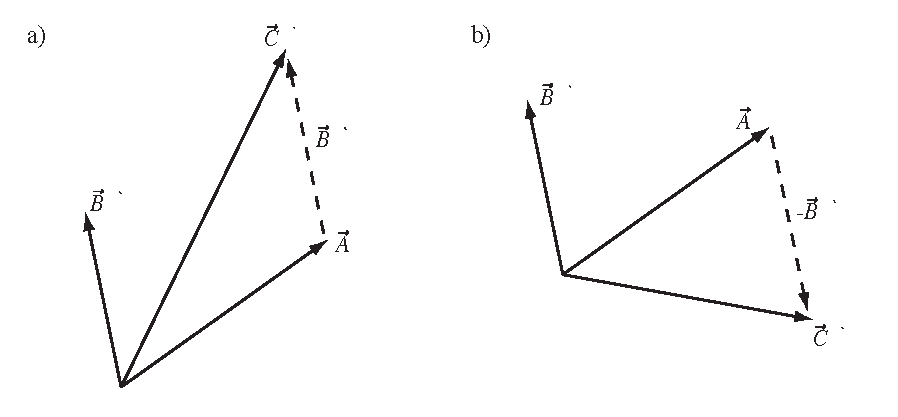
\epsfig{file=VectorOperations.pdf, width=\textwidth}
\caption{{\it (a) Optellen van vectoren. (b) Aftrekken van vectoren }}
\label{fig:vecop}
\end{center}
\end{figure}

Optellen van vectoren is bijvoorbeeld van belang
als je wil uitrekenen wat een positie van een object is na verschillende stappen te hebben
afgelegd, of voor het uitrekenen van een resultante kracht als er meerdere krachten op
ons object werken.

Voor het aftrekken van twee vectoren, $\vec{A}$ en $\vec{B}$, geldt:
\begin{eqnarray}
\vec{C} & = & \vec{A} - \vec{B} \\
              & = & (A_x - B_x,\, A_y - B_y, \,A_z - B_z) 
\end{eqnarray}
Grafisch is het aftrekken van twee vectoren weergegeven in Fig.~\ref{fig:vecop}~b). De resultante
vector $\vec{C}$ wordt verkregen door $\vec{B}$ van richting om te draaien en deze vervolgens
aan de punt van $\vec{A}$ te leggen.

De lengte van een vector kan eenvoudig worden berekend met behulp van onze klassieke
vriend Pythagoras. Voor een vector $\vec{A}$ is de lengte dus gegeven door:
\begin{equation}
|\vec{A}|  = \sqrt{A_x^2+A_y^2+A_z^2}  
\end{equation}
Met de lengte van een vector bekend, kan je vervolgens een vector maken die dezelfde
richting heeft als de originele vector $\vec{A}$, maar met lengte 1:
\begin{eqnarray}
\hat{A} & = & \frac{\vec{A}}{|\vec{A}|} \\
             & = & \left(\frac{A_x}{|\vec{A}|},\, \frac{A_y}{|\vec{A}|},\, \frac{A_z}{|\vec{A}|}\right)
\end{eqnarray}
Vectoren met lengte~1 worden {\bf eenheidsvectoren} genoemd, en ze worden onder andere
gebruikt om de richting van een vector aan te geven. Daarnaast kunnen we eenheidsvectoren gebruiken om een willekeurige andere vector te schrijven. Voor het definieren van een willekeurige vector in cartesische co\"{o}rdinaten kan het handig zijn de eenheidsvectoren te definieren, \ihat, \jhat en \khat die de richting van respectievelijk de $x$-as, de $y$-as en de $z$ aangeven.  Onze vertrouwde vector $\vec{A}$ kan met behulp van deze eenheidsvectoren worden geschreven als:
\begin{equation}
\vec{A} = (A_x,\,A_y,\,A_z) = A_x\,\ihat + A_y \, \jhat + A_z \khat
\end{equation}
Merk op dat de vectoren die we kiezen om een co\"{o}rdinatensysteem - in dit geval het cartesische - te beschrijven loodrecht op elkaar staan.  Ook bij andere keuzen van de co\"{o}rdinaten die we later in de college's tegenkomen is dit het geval. ({\it kennen jullie andere co\"{o}rdinatensystemen dan het cartesische? zo nee, zou je iets kunnen bedenken?})

Bovenstaande opmerking kunnen we formeel bewijzen door het introduceren van het vector scalar product of inproduct. Als je twee vectoren $\vec{A}$ en $\vec{B}$ hebt dan is het inproduct gedefinieerd als:
\begin{equation}
\vec{A}\cdot\vec{B} \equiv A_x B_x + A_y B_y + A_z B_z
\end{equation}
Let op de $\cdot$ tussen de twee vectoren die aangeeft dat er hier sprake is van een inproduct.
Laten we eens kijken wat het inproduct precies betekent. Ten eerste kan je opmerken dat we hier te maken hebben met een scalar. Het maakt dus niet uit hoe we tegen de vectoren $\vec{A}$ en $\vec{B}$ aankijken: we zouden bijvoorbeeld het gehele coordinatensysteem over een willekeurige hoek kunnen
draaien, waarbij $\vec{A}\rightarrow\vec{A}^{'}$ en $\vec{B}\rightarrow\vec{B}^{'}$. Wat we bedoelen met de uitspraak dat het inproduct {\it invariant} is onder een willekeurige rotatie is wiskundig niets anders dan:
\begin{equation}
\vec{A}\cdot\vec{B} = \vec{A}^{'}\cdot\vec{B}^{'}
\end{equation}
Hier kunnen we handig gebruik van maken om een diepere betekenis toe te kennen aan ons inproduct. We kunnen er namelijk voor kiezen om het coordinatensysteem zodanig te draaien dat de vector $\vec{A}^{'}$ langs de $x$-as ligt van ons nieuwe coordinatensysteem. En vervolgens kunnen we nog een keer draaien om de $x$-as totdat de vector $\vec{B}^{'}$ in het $x-y$ vlak ligt, zoals aangegeven in Fig.~\ref{fig:inproduct}.
\begin{figure}[htbp]
\begin{center}
  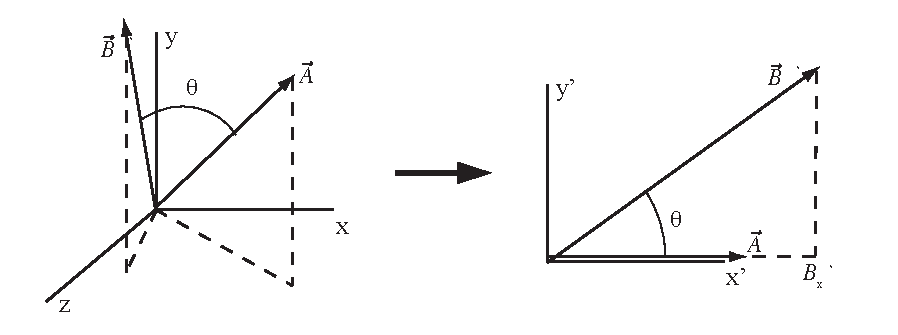
\epsfig{file=InnerProduct.pdf, width=\textwidth}
\caption{{\it Het inproduct van twee vectoren is invariant onder rotaties van het coordinatensysteem. }}
\label{fig:inproduct}
\end{center}
\end{figure} 
Voor het inproduct tussen de oude vectoren (!) geldt nu dus:
\begin{eqnarray}
\vec{A}\cdot\vec{B} & = & A_x^{'} B_x^{'} + 0 B_y^{'} + 0 B_z^{'} \\
                                   & = & |\vec{A}^{'}| |\vec{B}^{'}| \cos\theta^{'} \\
                                   & = & |\vec{A}||\vec{B}|\cos\theta \label{eq:inpr}
\end{eqnarray}
Hierbij is $\theta$ de hoek tussen de vectoren $\vec{A}$ en $\vec{B}$ en die is hetzelfde voor de geroteerde vectoren. Verder maken we er  gebruik van dat de lengte van een vector niet verandert bij een rotatie, en dat $A_x^{'}=|\vec{A}^{'}|$, omdat  deze vector langs de $x$-as wijst. Het inproduct van twee vectoren geeft je dus een manier om de hoek tussen de vectoren uit te rekenen. Daarnaast meet een inproduct de lengte van een vector in de richting van die andere vector (cryptische uitspraak die de moeite waard is om te begrijpen). 

Laten we ook eens kijken naar het inproduct van een vector met zichzelf. Aan de ene kant hebben we:
\begin{equation}
\vec{A}\cdot\vec{A} = A_x^2 + A_y^2 +A_z^2 
\end{equation}
En aan de andere kant hebben we dankzij Vgl.~\ref{eq:inpr}:
\begin{equation}
\vec{A}\cdot\vec{A} = |\vec{A}||\vec{A}|\cos 0 = |\vec{A}|^2
\end{equation}
En dat is gelukkig hetzelfde. Het inproduct van een vector met zichzelf geeft je dus de lengte van die vector in het kwadraat.
                                    
Tenslotte kan je direct aan het inproduct zien dat de eenheidsvectoren, \ihat, \jhat en \khat loodrecht op elkaar staan omdat:
\begin{equation}
\ihat\cdot\jhat=\ihat\cdot\khat=\jhat\cdot\khat = 0
\end{equation}
En dus klopt de belofte die we hierboven hebben gemaakt.

\section{Positie}

De eerste natuurkundige vector die we tegenkomen geeft de coordinaat van een object aan. We zullen voor een positie van een object in het kader van dit college altijd (of in ieder geval zoveel mogelijk) de volgende notatie aanhouden:
\begin{equation}
\vec{r}  \equiv (x, y, z)
\end{equation}
Niet echt wonderlijk, maar we kiezen ervoor om $x$, $y$ en $z$ te gebruiken voor de coordinaten.
Uiteraard kunnen we de positie ook weer schrijven als een som van eenheidsvectoren. Ten overvloede:
\begin{equation}
\vec{r} = x \ihat + y \jhat + z \khat
\end{equation}
Vaak zijn we niet direct geintereseerd in een positie zelf, maar in een verandering in positie. Een vector die je vaak tegenkomt in dat kader is de verplaatsingsvector, \dr, die is gedefinieerd als:
\begin{equation}
\dr \equiv \vec{r}_2 - \vec{r}_1
\end{equation}
De verplaatsingsvector wordt simpelweg verkregen door het aftrekken van twee vectoren zoals beschreven in de vorige paragraaf. Zoals duidelijk is in Fig.~\ref{fig:vecop}~b) wijst de vector \dr in de
richting van de $\vec{r}_2$ gezien vanaf de punt van $\vec{r}_1$. De vector \dr krijgt een duidelijke betekenis als we dadelijk posities definieren die veranderen als functie van de tijd ({\it wat zouden 
zulke vectoren ook alweer voorstellen?}).

\section{Snelheid en Impuls}

Een verandering van positie per eenheid van tijd kennen we uiteraard als snelheid. Om precies te zijn de instantane snelheid is gedefinieerd als de afgeleide van de positie naar de tijd. Dus de snelheid is:
\begin{equation}
\vec{v} \equiv \frac{d\vec{r}}{dt} = \left(\frac{dx}{dt}, \frac{dy}{dt}, \frac{dz}{dt}\right)
\end{equation}
Let er op dat snelheid net als de positie een vector grootheid is. Als je bij bijvoorbeeld een auto spreekt over de maximum snelheid die het beestje kan bereiken dan praat je over de maximale grootte die deze vector kan bereiken:
\begin{equation}
|\vec{v}| = \sqrt{\vec{v}\cdot\vec{v}}
\end{equation}
In het engels is het onderscheid tussen de grootte van de snelheid ('speed') en de vector snelheid ('velocity')  duidelijker. En ook als je een verschil in snelheid wil uitrekenen, moet je net
als voor de positie het verschil tussen twee snelheidsvectoren berekenen:
\begin{equation}
\dv = \vec{v}_2 - \vec{v}_1
\end{equation} 
De snelheid is uiteraard een extreem belangrijke grootheid als je een fysich systeem wil beschrijven. Vaker nog dan de snelheid zelf gebruiken natuurkundigen het begrip impuls. In de klassieke mechanica is de impuls niets anders dan de snelheid van een object  maal zijn massa:
\begin{equation}
\vec{p} \equiv m \vec{v}
\end{equation}
De impuls is als het ware een maat voor de 'hoeveelheid beweging'. Een van de redenen dat impuls zo'n enorm belangrijke grootheid is, is dat impuls ook buiten de klassieke mechanica universeel kan worden gebruikt, terwijl snelheid soms minder bruikbaar is. Het blijkt dat impuls een zogenaamde behouden grootheid is (dat zien we later in college nog weer terug) en dat er een mooie relatie is tussen impuls en het begrip kracht dat we in het volgende hoofdstuk behandelen.

\begin{center}
\line(1,0){250}
\end{center}
\begin{voorbeeld} 
\label{ex:student}
Op weg naar zijn vakantie in Spanje besluit een student op het dak van de bus te klimmen om 
indruk te maken op zijn jaarclubgenootjes. De bus rijdt met snelheid $v_b$ en de student klimt met 
snelheid $v_h$ op het dak van de bus. Wat is zijn snelheid ten opzichte van een argeloze 
toeschouwer? En onder welke hoek beweegt ie?

{\bf Oplossing} {\it We kiezen ervoor om de bus te laten rijden in de $x$-richting, 
dus $\vec{v}_b=(v_b,\,0,\,0)$
en de student klimt met snelheid $\vec{v}_s = (0,0,v_s)$ op het dak. Een stilstaande toeschouwer 
ziet de student dus met $v = (v_b,\,0,\,v_s)$ bewegen. Voor de hoek waaronder de student 
beweegt geldt nu dus eenvoudig: $\tan\theta = v_s / v_b$. Als de toeschouwer zelf ook nog 
beweegt kan je de snelheidsvector van zijn eigen beweging er ook nog bij optellen en zo voorts
}
\end{voorbeeld}

\begin{center}
\line(1,0){250}
\end{center}

\section{Versnelling}

De laatste vector die je nodig hebt om de beweging van een deeltje te karakteriseren is de 
zogenaamde versnelling. Een versnelling is niets anders dan de verandering van snelheid per 
eenheid van tijd. Deze is dus gedefinieerd als de eerste afgeleide naar de tijd van de snelheid, en 
dus de tweede afgeleide naar de tijd van de positie:
\begin{equation}
\label{eq:a}
\vec{a} \equiv \frac{d\vec{v}}{dt} = \frac{d^2\vec{r}}{dt^2} = \left(\frac{d^2x}{dt^2}, \frac{d^2y}{dt^2}, 
\frac{d^2z}{dt^2}\right)
\end{equation}
Versnelling is een begrip dat lastiger is dan het er op het eerste gezicht uitziet: zeker als je met de 
vectoren aan de slag gaat. Je zou op het eerste gezicht denken dat een versnelling altijd gepaard 
gaat met een verandering van de grootte van de snelheid, maar dit is niet altijd het geval. Dit is 
alvast een voorwaarschuwing dat je goed moet uitkijken met versnellingen en het is aan jullie om 
eens te denken onder welke omstandigheden een versnelling de grootte van de snelheid 
onveranderd laat. In ieder geval is het zo dat als de versnelling gelijk is aan nul een object beweegt 
met een {\it constante} snelheid in een {\it rechte} lijn.


\section{Eenparig versnelde beweging} \label{sec:eenparig}

Onder een eenparig versnelde beweging verstaan we een beweging waarvoor de
versnelling $\vec{a}$ constant is. Als $\vec{a}$ bekend is dan kunnen zowel de snelheid
$\vec{v}$ als de positie $\vec{r}$ worden uitgerekend als functie van de tijd, $t$. 

Laten we eerste eens kijken naar de snelheid als functie van de tijd. Stel dat op tijdstip
$t=t_0$ de snelheid $\vec{v}=\vec{v}_0$ bekend is, dan kunnen we door te integreren de 
snelheid uitrekenen als functie van de tijd ({\it let op de variabelen: er komen zowel $t$ als $t'$
voor in de vergelijkingen! weet je waarom?}) :
\begin{eqnarray}
\vec{v}(t) - \vec{v}_0 & = & \int_{t^{'}=t_0}^{t^{'}=t} \vec{a} \, dt^{'} \Rightarrow \\
\vec{v}(t)                     & =  & \vec{a} \, (t-t_0) + \vec{v}_0
\end{eqnarray}
Dus als je op $t=t_0$ de snelheid van een object weet, en je weet dat de versnelling constant is,
dan kan je de snelheid op een willekeurig tijdstip oplossen! De plaats als functie van de tijd 
kan worden bepaald door de snelheid nogmaals te integreren:
\begin{eqnarray}
\vec{r}(t) - \vec{r}_0 & = & \int_{t^{'}=t_0}^{t^{'}=t} \vec{v}\,dt^{'} \\
                                   & = &  \int_{t^{'}=t_0}^{t^{'}=t}  (\vec{a} \, (t^{'}-t_0) + \vec{v}_0) \,dt^{'} \Rightarrow \\
\vec{r}(t)                    & = & \frac{1}{2} \vec{a} (t-t_0)^2 +\vec{v}_0 \,(t-t_0) + \vec{r}_0 \label{eq:rt}
\end{eqnarray}
Deze vergelijking beschrijft eenparig versnelde beweging gegeven een beginsnelheid en positie. 
Waarschijnlijk heeft een aanzienlijk deel van jullie deze vergelijking al gezien op de middelbare school 
voor beweging in 1-D en met $t_0=0$.  In vectorvorm is de vergelijking algemeen geldig in 3-D.
Uiteraard wordt de situatie een stuk ingewikkelder als de versnelling niet constant
is. De integralen kunnen dan niet meer zo mooi worden opgelost: het is de moeite je te realiseren
dat eenparig versnelde beweging eerder een uitzondering is dan regel. De reden dat eenparig
versnelde beweging toch veel aandacht krijgt is dat de oplossing eenvoudig is: een simpele parabolische baan.

Voor alle duidelijkheid: wat we hierboven hebben gedaan is het oplossen van een $2^{\mathrm{e}}$ orde 
differentiaalvergelijking, namelijk  Vgl.~\ref{eq:a} . Een vergelijking dus waarin dubbele afgeleiden naar de tijd 
van de positie voorkomen. Een van de dingen die je ziet is dat je voor een complete oplossing van $\vec{r}(t)$ dan ook 2 
randvoorwaarden nodig hebt. In ons geval zijn dat $\vec{v}_0$ en $\vec{r}_0$. Een standaard methode om na te gaan of de
gevonden oplossing juist is, is (i) het expliciet invullen van de randvoorwaarden en (ii) het invullen van de oplossing in de
oorspronkelijke differentiaalvergelijking. 

\begin{center}
\line(1,0){250}
\end{center}

\begin{voorbeeld} 
\label{ex:parabool}
Een kogel wordt op $t=t_0$ afgeschoten vanaf positie $\vec{r}_0 = (x_0,\,y_0,\,0)$ met beginsnelheid 
$|\vec{v}_0=v_0$ onder een hoek $\theta$ zoals aangegeven in Fig.~\ref{fig:ex1}. Bereken (i) $\vec{r}(t)$, (ii) de 
tijd $T$ waarop de kogel de grond ($z=0$) weer raakt, en (iii) de snelheid waarmee de kogel de grond raakt. 
\begin{figure}[htbp]
\begin{center}
  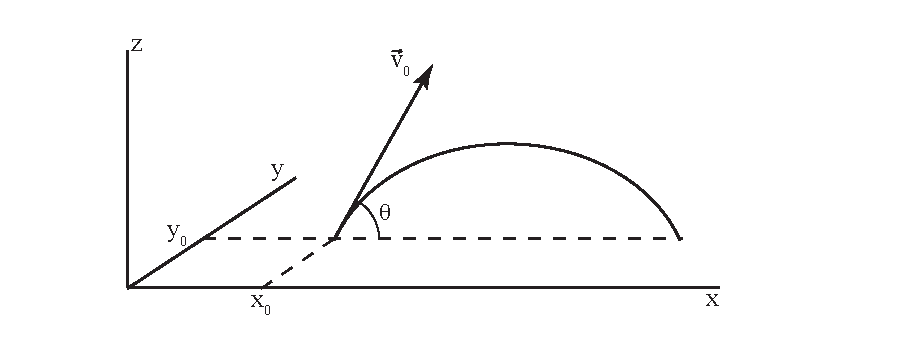
\epsfig{file=Paraboolbaan.pdf, width=\textwidth}
\caption{{\it Kogelbaan. }}
\label{fig:ex1}
\end{center}
\end{figure} 

{\bf Oplossing} {\it (i) Neem aan dat alleen de zwaartekrachtsversnelling $\vec{a}=(0,\,0,\,-g)$ een rol speelt in 
deze beweging. De snelheid $\vec{v}_0$ kan worden berekend uit de hoek $\theta$ en $v_0$ als 
$\vec{v_0} = v_0 (\cost,\,0,\,\sint)$. Invullen in vgl.~\ref{eq:rt} levert ons voor de 3 componenten 
van de positie:
\begin{equation}
\vec{r}(t) =
\left(\begin{array}{c}
0 \\
0 \\
-\frac{1}{2}\, g\,\dt^2
\end{array}\right)
+
\left(\begin{array}{c}
v_0 \cost \, \dt\\
0 \\
v_0 \sint \, \dt
\end{array}\right) 
+
\left(\begin{array}{c}
           x_0 \\
           y_0 \\
           0     \\
\end{array}\right)
\end{equation}
Met $\dt = t-t_0$. Je ziet dat we door het gebruik van vectoren te maken hebben met drie vergelijkingen (i.p.v. maar 1)
en dat ze alledrie verschillend zijn. De waarde van $y$ is constant: er is geen initiele snelheid in de $y$ richting en ook 
geen versnelling. De $x$ waarde neemt lineair toe met de tijd, omdat er een initiele snelheid is in de $x$ richting, maar
geen versnelling. Alleen de $z$ coordinaat wordt beschreven door een parabool, omdat de versnelling alleen in de $z$
richting wijst. (ii) Nu berekenen we de tijd waarop de kogel weer de grond raakt. Als de kogel de grond raakt geldt $z=0$,
ofwel:
\begin{eqnarray}
0 & = & -\frac{1}{2} g \dt^2 + v_0 \sint \dt \Rightarrow \\
\dt = 0 & \vee & \dt = \frac{2 v_0 \sint}{g}
\end{eqnarray}
De eerste oplossing komt overeen met het moment van afschieten van de kogel. De $z$ positie is 
dan immers  nul (randvoorwaarde). De tweede oplossing komt overeen met het moment dat de 
kogel de grond weer raakt (vraag: kloppen
de eenheden?). (iii) Doe dit zelf maar eens.
}
\end{voorbeeld}

\begin{center}
\line(1,0){250}
\end{center}

\section{Wat moet ik weten en kunnen?}

De volgende begrippen moet je tot je nemen:
\begin{itemize}
\item Verschil tussen vectoren en scalairen.
\item Wat zijn eenheidsvectoren?
\item Wat is de relatie tussen $\vec{r}$, $\vec{v}$ en $\vec{a}$?
\item Eenparig versnelde beweging.
\end{itemize}
En hiermee moet je kunnen rekenen:
\begin{itemize}
\item Vectoren: optellen, aftrekken en inproduct.
\item Banen van eenparig versnelde objecten.
\end{itemize}

\section{Opdrachten}

Hint voor het maken van de opgaven uit Giancoli: vervang alle getallen door variabelen. Op het 
tentamen wordt van je verwacht dat je kan rekenen met symbolen. Specifiek voor de vragen over 
objecten in een paraboolbaan: neem aan dat de zwaartekracht-versnelling wordt gegeven door $
\vec{a} = -g~\khat$.
\begin{enumerate}
\item Je kan alle opgaven bij Hfd.3 van Giancoli proberen te maken.
\item Speciale selectie uit Hfd.3 "General Problems". In ieder geval maken: 72, 75, 77, 78, 81, 83~(moeilijk),  87, 88, 93, 95.   
\item Bewijs vgl.~\ref{eq:inpr}.
\item Bewijs dat vgl.~\ref{eq:rt} zowel voldoet aan de differentiaalvergelijking in vgl.~\ref{eq:a} als 
aan de randvoorwaarden.
\item Onder welke hoek $\theta$ komt de kogel in voorbeeld~\ref{ex:parabool} het verste in $x$? 
(Hint: gebruik $\sin 2\theta = 2\sin\theta\cos\theta$.)
\item Geef een uitdrukking voor de afgelegde afstand $\Delta x$ in voorbeeld~\ref{ex:parabool} 
wanneer de kogel niet vanaf $z=0$, maar vanaf hoogte $h$ wordt afgeschoten.
\item Bereken weer de hoek $\theta$ waaronder de kogel het verste komt.
\end{enumerate}

%%%%%%%%%%%%%%%%%%%%%%%%%%%%%%%%%%%%%%%%%%%%%%%
% EINDE BEWEGING in 3-D
%%%%%%%%%%%%%%%%%%%%%%%%%%%%%%%%%%%%%%%%%%%%%%%

%%%%%%%%%%%%%%%%%%%%%%%%%%%%%%%%%%%%%%%%%%%%%%%
% BEGIN NEWTON's WETTEN
%%%%%%%%%%%%%%%%%%%%%%%%%%%%%%%%%%%%%%%%%%%%%%%

\chapter{Newton's wetten}\label{chap:newton}

In dit hoofdstuk komen de drie wetten van Newton aan bod. Deze wetten vormen het hart
van de klassieke mechanica en sommige begrippen zijn houdbaar ook buiten
de klassieke mechanica. De wetten van Newton vormden een revolutie in de
natuurwetenschappen en hebben de basis gelegd voor de exacte - mathematische - beschrijving
van de natuur zoals we die nu kennen.

Naast de wetten van Newton zelf worden in dit hoofdstuk een paar veel in de natuur 
voorkomende krachten behandeld.

Stof uit Giancoli:
\begin{itemize}
\item Hoofdstuk 4
\item Hoofdstuk 5.1 en 5.6
\end{itemize}

\section{Eerste wet {\it of }  "Dat eens roert, roert altijt, soot niet belet wort"}\label{sec:newton1}

De eerste van de drie wetten van Newton is een uitspraak over de relatie tussen krachten en
beweging van een object. 

\begin{Newton1}
Een object waarop de netto kracht gelijk is aan nul, beweegt met een constante snelheid (of is en blijft in rust).
\end{Newton1}

De eerste wet van Newton vertelt ons dus dat als we de snelheid van een object willen 
veranderen, daarvoor een kracht nodig is. Heel simplistisch gezien lijkt het bijna
een betekenisloze uitspraak: je moet iets doen om iets te veranderen. Toen Newton
zijn eerste wet op schrift stelde, was het echter niet minder dan een revolutionaire gedachte
(eerlijk is eerlijk: Galilei had hetzelfde idee ook min of meer gehad, maar dat was dan ook
een behoorlijk slimme kerel). Eeuwenlang had men het gedachtegoed van Aristoteles en zijn 
oude Griekse vrienden gekoesterd en die beweerden het tegenovergestelde: namelijk dat
elk object een 'natuurlijke drang' heeft om tot rust te komen en dat je zelf iets moet doen
om een beweging aan de gang te houden.  Deze kijk op de natuur is natuurlijk niet zo wonderlijk, 
omdat dat strookt met onze dagelijkse waarnemingen. Als je een willekeurig object een zetje geeft 
komt ie in beweging en stopt ie na een meestal korte tijd weer. Newton verklaart dit tot stilstand
komen niet met een natuurlijke drang, maar uit het feit dat er {\it dus} een kracht op dit object werkt.
({\it vraag: een schaatser maakt snelheid, glijdt een eindje en komt tot stilstand. Verklaar zowel 
aan de had van de oude Grieken en aan de hand van Newton en Galilei.})

Het is van belang te onderzoeken wanneer Newtons eerste wet geldt. Wanneer je in 
een trein zit die versnelt en er ligt een bal op de vloer, dan versnelt die bal , zonder dat er 
een kracht op die bal lijkt te werken. In versnelde systemen werkt Newton's eerste wet 
blijkbaar niet ({\it vraag: is dat vreemd?}). In het algemeen geldt Newton's eerste wet in systemen 
die met een constante snelheid ten opzichte van elkaar bewegen: ook 'stilstaande' systemen
zijn hiervoor dus prima geschikt. Vaak nemen we een stilstaand coordinatensysteem
dat we definieren ten opzichte van een vast punt op het oppervlak van de aarde als 
referentiesysteem, hoewel dat niet helemaal correct is ({\it waarom niet?}). Dergelijke systemen,
waarin de eerste wet van Newton geldt noemen we {\bf inertiaalstelsels}. 

\section{Tweede wet}

De eerste wet van Newton legt een relatie tussen kracht en snelheidverandering. Newton's
tweede wet legt vast hoe die relatie precies in elkaar zit.
\begin{Newton2}
De versnelling van een object is evenredig met de netto kracht die op het object wordt
uitgeoefend:
\begin{equation}\label{eq:newton2}
\vec{F}_{tot} = \sum \vec{F} = m \vec{a}
\end{equation}
\end{Newton2}
De evenredigheidsconstante tussen de kracht en de versnelling is wat wij kennen
als de massa, $m$, van dat object.  Een grote massa is moeilijker in beweging te krijgen
dan een kleine massa. Een grote kracht leidt tot een grote versnelling. Precies zoals we 
verwachten dus.  De meesten van jullie kunnen we op een willekeurig moment wel 
wakker maken voor opdreunen van deze formule, maar toch is dit niet de meest gebruikelijke
notatie voor het schrijven van Newton's tweede wet. Als we het begrip impuls, 
$\vec{p}=m\vec{v}$ uit het vorige hoofdstuk er weer bij halen, en de afgeleide nemen naar
de tijd, zie je dat we vgl.~\ref{eq:newton2} ook kunnen schrijven als:
\begin{equation}
\vec{F}_{tot} = \frac{d \vec{p}}{dt}
\end{equation}
In deze vorm wordt de tweede wet van Newton het liefst gebruikt: een kracht leidt tot
een verandering van impuls. Deze relatie tussen impuls en kracht maakt impuls zo'n enorm
belangrijke grootheid binnen de klassieke mechanica en daarbuiten. De tweede wet van Newton
is perfect consistent met  de eerste wet - eigenlijk is het een meer wiskundige manier van hetzelfde
statement. Wanneer de kracht in vgl.~\ref{eq:newton2} gelijk aan nul is, is de versnelling
nul, en de snelheid dus constant. Net zoals de eerste wet je vertelt.

\begin{center}
\line(1,0){250}
\end{center}

\begin{voorbeeld} 
\label{ex:newton:kracht}
 \begin{figure}[htbp]
\begin{center}
  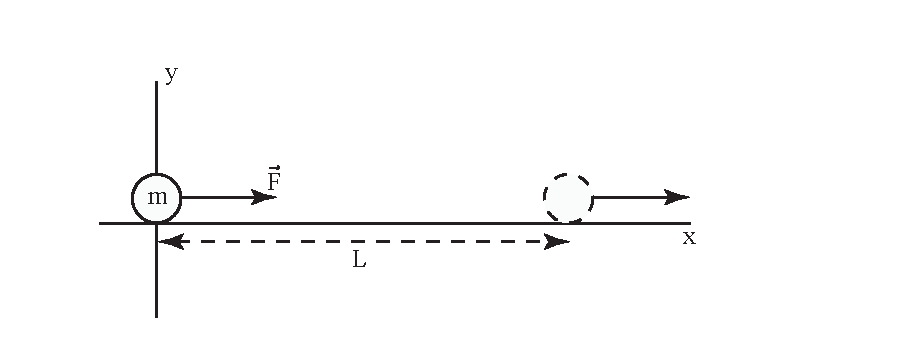
\epsfig{file=Versnelling.pdf, width=\textwidth}
\caption{{\it Kracht en versnelling.}}
\label{fig:newton:wet2}
\end{center}
\end{figure} 
Je trekt met een kracht $\vec{F}$ aan een object met massa $m$. Van wrijving of andere
soorten weerstand is geen sprake. Hoe lang doe je er over om een afstand $L$ af te leggen als
het object op $t=0$ in rust is?

{\bf Oplossing: }{\it Laten we ervoor kiezen om de kracht op ons object te laten werken in de $x$ richting,
 zoals aangegeven in Fig.~\ref{fig:newton:wet2}: er geldt dan $\vec{F} = (F, \, 0,\,0)$. 
 De versnelling wordt
 dan gegeven door $\vec{a}=(F/m, \,0,\,0)$. Als we nu de vergelijking voor eenparig versnelde beweging
 weer uit de kast halen krijgen we:
 \begin{equation}
 \vec{r}(t) = \left(\begin{array}{c}
  x(t) \\
  y(t) \\
  z(t) 
  \end{array}\right)
  = \frac{1}{2}\left(\begin{array}{c}
  (F/m) \, t^2 \\
  0 \\
  0
 \end{array}\right)
  + \vec{0} \, t + \vec{0}
 \end{equation}
 De laatste twee vectoren geven aan dat de initiele snelheid nul is, $\vec{v}_0 = \vec{0}$ en dat de initiele
 positie van het object in de oorsprong ligt $\vec{r}_0 = \vec{0}$. Deze laatste heb ik zo gekozen uit gemak.
 Oplossen voor $x(t)=L$ geeft:
 \begin{equation}
 t = \sqrt{\frac{2 \,m \,L}{F}}
 \end{equation}
 Vraag: check of de dimensies kloppen.
 }
\end{voorbeeld}

\begin{center}
\line(1,0){250}
\end{center}


\section{Derde wet}

De derde wet van Newton behandelt de vraag hoe nou precies krachten worden uitgeoefend
tussen objecten. Newton heeft dit mechanisme samengevat in zijn bekende actie is reactie wet:
\begin{Newton3}
Als een object een kracht uitoefent op een tweede object, dan oefent dat tweede object een
evengrote kracht uit op het eerste object in tegengestelde richting.
\end{Newton3}
of:
\begin{equation}
\vec{F}_{1\rightarrow2} = - \vec{F}_{2\rightarrow1}
\end{equation}
Op het eerste gezicht lijkt deze wet triviaal, want als ik bijvoorbeeld stil op de grond sta, dan
trekt de zwaartekracht mij naar beneden, terwijl de grond even hard naar boven duwt. De 
totale kracht op mij is gelijk nul, en ik blijf dus onversneld (=stil) staan. Maar Newton postuleerde
dat ook als een object wel versneld wordt, de kracht die zorgt voor de versnelling een even
grote reactie-kracht opwekt.

Je zou jezelf nu de vraag kunnen stellen hoe het mogelijk is dat er uberhaupt iets in 
beweging gezet kan worden, aangezien de som der krachten altijd nul is. Voor iedere
kracht is er immers een reactiekracht van tegengesteld teken. Het antwoord op die vraag
ligt in het feit dat je je altijd moet afvragen {\it waarop} een bepaalde kracht wordt uitgeoefend.
Als ik bijvoorbeeld een krijtje het publiek in wil gooien tijdens een college, dan oefen ik
daarvoor een kracht uit op het krijtje. De reactiekracht volgens Newton's derde wet is tegengesteld
aan deze kracht, maar deze wordt uitgeoefend op mijn hand en niet op het krijtje. Op
het krijtje wordt dan wel degelijk een netto kracht uitgeoefend en daardoor wordt deze 
versneld.

Het voorbeeld hierboven van het krijtje wordt trouwens op grote schaal gebruikt bij
voortstuwing van bijvoorbeeld raketten. Een raket stoot
enorme hoeveelheden gassen met een hoge snelheid uit de motor. Bij deze
uitstoot worden de gassen enorm versneld en de raket oefent dus een grote kracht
uit op deze gassen. Volgens Newton's derde wet is er een reactiekracht even groot in 
tegengestelde richting die wordt uitgeoefend op de raket door deze gassen. Het is precies
deze reactiekracht die ervoor zorgt dat een raket zich voortbeweegt, en niet zoals je
vaak hoort door het afzetten van de gassen tegen de grond of de omliggende lucht. Stel dat een
raket zich wel zou afzetten tegen de atmosfeer of de grond. Hoe zou zo'n beest dan moeten
versnellen als ie eenmaal buiten de dampkring is?

\section{Krachten van verschillende soorten}

In deze paragraaf passeren er verschillende typen krachten de revue met als doel dat je het
gereedschap hebt om eenvoudige krachten analyses te doen. Een dergelijke krachten analyse
volgt altijd min of meer hetzelfde patroon. Je begint met een schets te maken van het fysische
probleem, waarmee wordt bedoeld een tekening van alle relevante objecten en krachten die
worden uitgeoefend. Als je hebt geanalyseerd welke krachten van belang zijn, ben je in staat
de netto-kracht en dus versnelling van een object uit te rekenen. Meestal is de wiskunde voor
dergelijke problemen eenvoudig. Wat lastig is, is een goede en trefzekere analyse van het 
probleem om de krachten op je object te bepalen. Uiteraard moet je er bij dergelijke analyses altijd
rekening mee houden dat je te maken hebt met vectoren. In de rest van de paragraaf worden 
meer en meer krachten geintroduceerd en zal je in staat zijn ingewikkelder problemen op
te lossen.

\subsection{Zwaartekracht \& Normaalkracht}

De eerste kracht die aan bod komt zal niet verrassend de zwaartekracht zijn. Bij de problemen
die we in dit hoofdstuk tegenkomen zal de zwaartekracht, $\vec{F}_G$ op een object met massa
$m$  worden gegeven door:
\begin{equation}\label{eq:zwaartekracht}
\vec{F}_G = m \vec{g}
\end{equation}
waarbij $\vec{g}=(0,\,0,\,-9.8m/s^2)$ de zwaartekrachtsversnelling aan het oppervlak van de aarde.
Let hierbij op het min-teken voor de zwaartekrachtsversnelling, aangezien ik de positieve
$z$-as van mijn coordinaten systeem het liefste omhoog laat wijzen.  Let wel goed op dat
vgl.~\ref{eq:zwaartekracht} alleen geldig is aan het oppervlak van de aarde. Wanneer we de ruimte in
gaan dan moeten we Newton's zwaartekrachtwet gebruiken die netjes de zwaartekracht  beschrijft
als functie van de afstand tot een object (bv. de aarde). Ook als we opgaven gaan doen op een 
andere planeet moet je ermee rekening houden dat $\vec{g}$ wel eens anders kan zijn. 
Het is trouwens wel opmerkelijk (dat vond Einstein tenminste) dat de massa die horen bij
de tweede wet van Newton, $\vec{F}=m\vec{a}$ precies dezelfde massa is als die hoort
bij de zwaartkrachtvergelijking~\ref{eq:zwaartekracht}. Het gevolg is dat objecten ongeacht
hun massa precies dezelfde versnelling ondergaan! Deze equivalentie tussen {\it trage} en
{\it zware} massa is tot op grote nauwkeurigheid experimenteel aangetoond en vormt
een van de fundamenten van de algemene relativiteitstheorie van Einstein.

Een vaste partner van de zwaartekracht is de zogenaamde normaalkracht. Als docent Colijn
met zijn volle gewicht op de grond staat werkt de zwaartekracht op hem, terwijl hij toch niet
door de grond zakt. De kracht die terugduwt heet de normaalkracht, meestal weergegeven
door $\vec{F}_N$. 
 \begin{figure}[htbp]
\begin{center}
  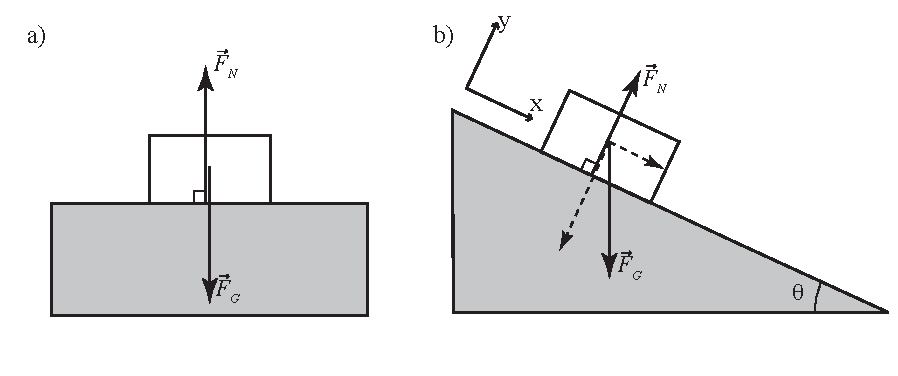
\epsfig{file=NormaalKracht.pdf, width=\textwidth}
\caption{{\it a) Zwaartekracht en normaalkracht voor een horizontaal oppervlak. b) Hetzelfde maar
nu voor een oppervlak dat onder een hoek $\theta$ staat.}}
\label{fig:norm}
\end{center}
\end{figure} 
De normaalkracht staat {\it altijd} loodrecht op het oppervlak dat deze kracht uitoefent,
dus als het oppervlak waarop een object zich bevind horizontaal is, zal de normaalkracht 
precies even groot zijn als de zwaartekracht zoals aangegeven in Fig.~\ref{fig:norm}~a). 
Wat verder belangrijk is om  te zien in Fig.~\ref{fig:norm} is waar de zwaartekracht en de 
normaalkracht aangrijpen. De zwaartekracht wordt altijd getekend vanuit het zwaartepunt of 
massa-middelpunt (wordt later nog behandeld), terwijl de normaalkracht aangrijpt bij het contact
tussen het oppervlak en het object.

Als  het object - Colijn in dit geval - zich op een hellend vlak begeeft wijst de normaalkracht 
nog steeds
loodrecht op het oppervlak, zodanig dat de component van de zwaartekracht in de richting van het 
oppervlak precies wordt opgeheven, zoals in Fig.~\ref{fig:norm}b).  Wat denk je dat er zou 
gebeuren als dit niet het geval zou zijn? Mochten er verder geen wrijving 
of andere krachten in het spel zijn dan zorgt de component van de zwaartekrachtsversnelling 
langs de helling voor de versnelling van de docent. Realiseer je wel dat niet alleen de 
zwaartekracht een normaalkracht kan veroorzaken: ook als je bijvoorbeeld hard tegen een muur 
aanduwt zorgt de normaalkracht, die even grot is als de kracht waarmee je duwt, ervoor dat je 
hand niet door de muur heengaat.

\begin{center}
\line(1,0){250}
\end{center}

\begin{voorbeeld} 
\label{ex:normaalkracht}
Stel dat de massa van het object op de helling in Fig.~\ref{fig:norm} gegeven is door $m$. 
Wat is (i) de normaalkracht op het object (ii) de versnelling? 

{\bf Oplossing: } {\it De normaalkracht is de reactiekracht die de component van de zwaartekracht 
loodrecht op het oppervlak compenseert. Het is in dit geval handig om een coordinatensysteem te 
kiezen waarbij de $x$-as parallel aan het schuine oppervlak staat en de $y$-as loodrecht daarop. 
(i) In dit coordinatensysteem geldt voor de normaalkracht:
\begin{equation}
\vec{F}_N = m \, g \left(\begin{array}{c}\
0 \\
\cos\theta
\end{array}\right)
\end{equation} 
De grootte van $\vec{F}_N$ is dus $m\,g\,\cos\theta$. (ii) Voor de grootte van de kracht langs het
oppervlak geldt dan $|\vec{F}_{par}|=m\,g\,\sin\theta$ en voor de versnelling hoeft nog slechts
gedeeld te worden door $m$.
 }
\end{voorbeeld}
\begin{center}
\line(1,0){250}
\end{center}

Een laatste belangrijke opmerking over normaalkrachten: dit zijn de krachten die uiteindelijk
bepalen hoeveel gewicht je aangeeft op een weegschaal. Namelijk door op een weegschaal
te gaan staan (moet wel horizontaal staan) zorgt de zwaartekracht ervoor dat de weegschaal
een normaalkracht op jou moet uitoefenen die gelijk is aan de zwaartekracht. Je meet dus
op een weegschaal dus ook niet je massa (hoewel die wel op het metertje staat aangegeven), 
maar je meet het effect van de zwaartekracht op jouw hoeveelheid massa. Als je de
weegschaal meeneemt naar de maan zal je slechts een fractie van je gewicht meten omdat
$g$ op de maan veel kleiner is. Je massa is natuurlijk hetzelfde gebleven (als je tenminste
niet bent afgevallen van de raketreis). 

\subsection{Spankracht}

Heel kort een veelvoorkomende kracht: de spankracht in een flexibel koord met
vaste lengte en massa $m=0$. Als je met een dergelijk touw aan een object trekt dan
kan je drie dingen direct opmerken over de krachten in het koord. Ten eerste moet
de kracht in het koord - spankracht of $\vec{F}_T$ genoemd - in dezelfde richting
staan als het koord zelf. Zou dit niet het geval zijn dan zorgt het koord er voor dat 
ie toch in de richting van de kracht komt te staan in de kleinst mogelijke tijd. Het
koord is immers flexibel en heeft $m=0$ ({\it probeer dit argument te begrijpen met
redenatie uit ongerijmde~\footnote{Bij een redenatie uit het ongerijmde laat je zien dat het tegendeel van 
je stelling leidt tot een contradictie}}). Ten tweede moet de krachten op beide uiteinden van
het koord hetzelfde zijn met tegengesteld teken.  Tenslotte kan je aan een dergelijk 
flexibel koord alleen maar trekken. Duwen met een draadje is niet mogelijk, maar
dat zal je wel niet verbazen.

\begin{center}
\line(1,0){250}
\end{center}
\begin{voorbeeld} 
\label{ex:spankracht}
Twee massa's $m_B$ en $m_A$ zijn met elkaar verbonden door middel van een touw. Je
trekt met kracht $\vec{F}_P$ aan de twee massa's zoals aangegeven in Fig.~\ref{fig:span}. 
Wat is (i) de versnelling van beide massa's en (ii) de spankracht in het touw als we ervan
uitgaan dat er geen wrijving is?

\begin{figure}[htbp]
\begin{center}
  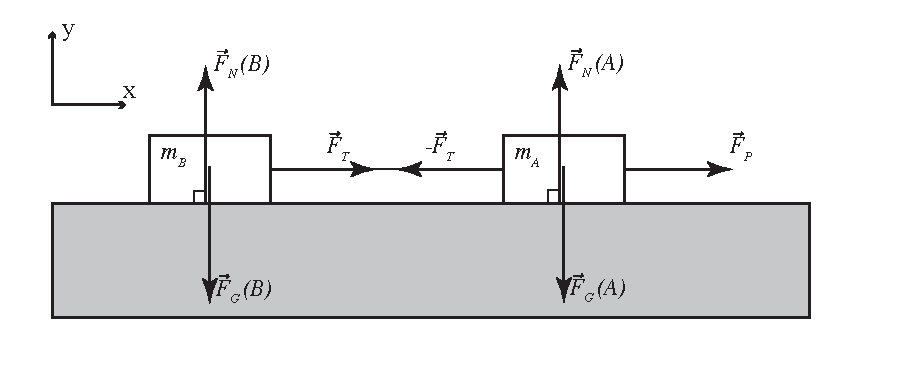
\epsfig{file=SpanKracht.pdf, width=\textwidth}
\caption{{\it Massa A en B worden voortgetrokken en zijn verbonden door middel van een touw.}}
\label{fig:span}
\end{center}
\end{figure} 
{\bf Oplossing: } {\it Begin bij het oplossen van een dergelijk probleem {\it altijd} met het
maken van een tekening van alle relevante krachten. Is ook belangrijk op een tentamen, omdat
er anders geen punten worden gegeven. We kijken eerst naar massa B en zien dat er in totaal
drie krachten op deze massa werken, een spankracht, de zwaartekracht en een normaalkracht.
Dus:
\begin{equation}
\vec{F}_T +\vec{F}_G(B)+\vec{F}_N(B)= m_B\, \vec{a}_B
\end{equation}
Het lijkt misschien een beetje overdreven om hier alle krachten op te schrijven, omdat we toch
niet echt geinteresseerd zijn in beweging in de $y$ richting. In de $y$-richting gebeurt er niet
zoveel zolang de massa's niet loskomen van het oppervlak: de normaalkracht heft precies de
zwaartekracht op. We kunnen ons in dit geval dus
net zo goed beperken tot het opschrijven van alleen de $x$ component van de krachten
en versnelling. Voor massa A en B wordt dit:
\begin{eqnarray}
F_{P\,x} - F_{T\,x} & = & m_A\,a_{A\,x}\\
F_{T\,x} & = & m_B\,a_{B\,x} 
\end{eqnarray}
Beide versnellingen moeten wel aan elkaar gelijk zijn $\vec{a}=\vec{a}_A=\vec{a}_B$, omdat het touw niet kan uitrekken. We
hebben dan twee vergelijkingen met twee onbekenden waaruit we (i) vinden
\begin{equation}
|\vec{a}| = \frac{|\vec{F}_P|}{m_A+m_B}
\end{equation}
en (ii) voor de spankracht:
\begin{equation}
|\vec{F}_T| = \frac{m_B}{m_A+m_B}\,|\vec{F}_P|
\end{equation}

 }
\end{voorbeeld}
\begin{center}
\line(1,0){250}
\end{center}

\subsection{Wrijving}\label{sec:wrijving}

Tot nu toe hebben we aangenomen dat alle beweging gebeurt zonder wrijving. Dit is
uiteraard een onhoudbare simplificatie van de meeste natuurkundige problemen in 
de klassieke mechanica, en zonder wrijving stroken de meeste berekeningen dan ook niet
met onze dagelijkse ervaringen. In deze paragraaf komt wrijving aan bod tussen twee
oppervlakken die met elkaar contact maken. We moeten bij wrijving een duidelijk
onderscheid maken tussen twee vormen van wrijving: {\it kinetische} en {\it statische}. 

Kinetische wrijving is de wrijvingskracht die een object ondervindt wanneer deze
langs een oppervlak beweegt. De wrijvingskracht, $\vec{F}_{fr}$~\footnote{Het subscript
$fr$ komt van het Engelse woord voor wrijving, friction. Deze notatie wordt gebruikt in
Giancoli.} is tegengesteld aan de richting van de beweging en de grootte is evenredig 
met de normaalkracht:
\begin{equation}
|\vec{F}_{fr}| = \mu_{k} |\vec{F}_N|
\end{equation}
De evenredigheidsconstante $\mu_k$ heet de coefficient van kinetische wrijving, en deze
moet empirisch worden bepaald. Een microscopisch model voor het uitrekenen van 
wrijvingskrachten is praktisch niet te realiseren, omdat je voor het uitrekenen van $\mu_k$ 
gecompliceerde grootheden als moleculaire aantrekkingskrachten, ruwheid van oppervlakten 
en dergelijke nodig hebt. Experimentele waarden voor $\mu_k$ liggen tussen 0.01 ({\it
wat zou de eenheid van $\mu$ zijn}) voor goed geoliede kogellagers tot 0.4 voor
bijvoorbeeld het bewegen van hout op hout.

Naast kinetische wrijving heb je uiteraard ook te maken met wrijving als je tegen een
object dat nog niet in beweging is: dit heet statische wrijving. Zolang een object niet
beweegt is de wrijvingskracht even groot als de kracht die werkt langs het oppervlak wordt
uitgeoefend. De maximale wrijvingskracht waarbij een object nog net niet in beweging komt
wordt gegeven door:
\begin{equation}\label{eq:wrijvingstatisch}
|\vec{F}_{fr}| = \mu_s |\vec{F}_N|
\end{equation}
Wederom is de kracht evenredig met de normaalkracht die het object uitoefent, maar
nu met de coefficient van statische wrijving, $\mu_s$. Dus denk 
er om dat de wrijvingskracht zolang een object stilstaat even groot is als de kracht die
wordt uitgeoefend langs het oppervlak. Vgl.~\ref{eq:wrijvingstatisch} geeft het \emph{maximum}
aan van deze kracht. In het algemeen geldt:
\begin{equation}\label{eq:wrijvingscoef}
\mu_s \geq \mu_k
\end{equation}
De statische wrijvingskracht is groter dan de kinetische. Dit strookt met dagelijkse ervaringen
als je bijvoorbeeld denkt aan het verschuiven van een zware doos op een parketvloer. Als
de doos eenmaal in beweging is kost het minder moeite om de doos in beweging te houden. 
Stel nou eens dat $\mu_s<\mu_k$. In dat geval zou de wrijvingskracht tijdens bewegen 
groter moeten zijn dan tijdens stilstand: het zal je dan niet lukken een object van z'n plek
te krijgen! Dus het moet wel zo zijn dat vgl.~\ref{eq:wrijvingscoef} geldt.

\begin{center}
\line(1,0){250}
\end{center}
\begin{voorbeeld} 
\label{ex:wrijving1}
Je trekt aan een object met massa $m$ net zo hard dat ie net in beweging komt, zoals
in Fig.~\ref{fig:wrijving1}~a). Wat is de versnelling als de coefficienten van statische en
kinetische wrijving respectievelijk $\mu_s$ en $\mu_k$ heten?
\begin{figure}[htbp]
\begin{center}
  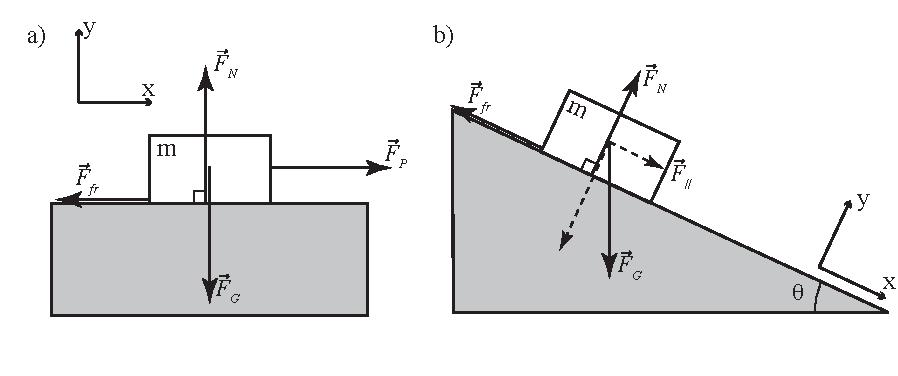
\epsfig{file=Wrijvingskracht.pdf, width=\textwidth}
\caption{{\it a) Wrijvingskracht in het horizontale vlak en b) op een hellend vlak.}}
\label{fig:wrijving1}
\end{center}
\end{figure} 

{\bf Oplossing: } {\it  Om het object te laten bewegen moet je trekken met een kracht
die tenminste net zo groot is als de maximale wrijvingskracht. Dus:
\begin{equation}
\vec{F}_P = (\mu_s |\vec{F}_N|,\,0,\,0) = (\mu_s\,m\,g,\,0,\,0)
\end{equation}
Maar op het moment dat het object begint te bewegen geldt dat de wrijvingskracht 
wordt gegeven door $|\vec{F}_{fr}| = \mu_k |\vec{F}_N|$. De netto kracht op het object wordt
gegeven door (de $y$ componenten heffen elkaar netjes op):
\begin{equation}
\vec{F}_{tot} = ((\mu_s-\mu_k)\,m\,g,\,0,\,0)
\end{equation}
Dus is er een versnelling in de $x$ richting van $a_x = (\mu_s-\mu_k)\,g$.
}
\end{voorbeeld}
\begin{center}
\line(1,0){250}
\end{center}
\begin{voorbeeld} 
\label{ex:wrijving2}
Een object met massa $m$ staat op een vlak met hellingshoek $\theta$, zoals in Fig.~\ref{fig:wrijving1}~b). 
Wat is de maximale hoek $\theta$ zodat het object net stil blijft liggen (de coefficient van statische wrijving 
heet weer $\mu_s$?

{\bf Oplossing: } {\it  Het object begint langs de helling glijden wanneer de kracht langs het oppervlak, $\vec{F}_{//}$ 
groter wordt dan de maximale wrijvingskracht. Dus.
\begin{eqnarray}
|\vec{F}_{//}| & = & |\vec{F}_{fr \,\, max}| \\
|\vec{F}_G|\,\sin\theta & = & \mu_s \, |\vec{F}_N| \\
m\,g\,\sin\theta & = & mu_s\,m\,g\,\cos\theta \\
& \Downarrow & \\
\tan\theta & = & \mu_s
\end{eqnarray}
Let er op dat je wordt geacht bij een dergelijke opgave \emph{zelf}  alle krachten, hoeken en dergelijke te tekenen.
}
\end{voorbeeld}
\begin{center}
\line(1,0){250}
\end{center}

\subsection{Snelheidsafhankelijke krachten}

De wrijvingskrachten beschreven in paragraaf~\ref{sec:wrijving} hangen alleen af van
de druk die een object uitoefent op een oppervlak. Objecten die vallen door een medium
ondervinden in het algemeen ook weerstandskrachten die een functie zijn van de snelheid. 
Deze krachten zijn van belang bijvoorbeeld voor de beweging
van een object door een vloeistof of een gas. Voor kleine objecten met lage 
snelheid wordt een dergelijk kracht in goede benadering gegeven door:
\begin{equation}\label{eq:drag}
\vec{F}_D = - \, b\,\vec{v}
\end{equation}
Het minteken geeft aan dat de kracht staat in de richting tegengesteld aan de 
bewegingsrichting van het object. De evenredigheidsconstante $b$ - die meestal
niet eens echt constant is - hangt af
van de stroperigheid, ook wel bekend viscositeit, van het medium en de vorm van het object.
({\it Vraag: wat is de eenheid van b?}). 

Als we te maken hebben met een dergelijke kracht wordt het oplossen van de positie als
functie van de tijd, $\vec{r}(t)$ lastiger, maar in sommige gevallen kunnen we wel een duidelijke
uitspraak doen wat er uiteindelijk gebeurt met een object. Een van die gevallen is wanneer
we te maken hebben met een object in vrije val door de lucht. In dat geval neemt de snelheid
als functie van de tijd snel toe, maar ook de wrijvingskracht. Na niet al te lange tijd
is er een situatie bereikt waarbij de wrijvingskracht precies even groot is als de zwaartekracht:
\begin{equation}\label{eq:vt}
\vec{F}_D - \vec{F}_G = m \, \vec{a} = m\,\vec{0}
\end{equation}
In dit geval is de eindsnelheid - eng. terminal velocity - $\vec{v}_T$ uit te drukken in bekende
grootheden:
\begin{equation}
\vec{v}_T = (0,\,0,\,-\frac{m\,g}{b})
\end{equation}
waarbij we aannemen dat de zwaartekracht in de $-z$ richting wijst. Hoe snel $\vec{v}_T$ wordt
bereikt hangt af van de grootte van $b$ in vergelijking tot de massa van een object. En als je
precies wil weten hoe de snelheid zich gedraagt als functie van de tijd moet je vgl.~\ref{eq:vt}
oplossen ook voor $\vec{a}\neq\vec{0}$.

\begin{center}
\line(1,0){250}
\end{center}
\begin{voorbeeld} 
\label{ex:drag}
We laten een object met massa $m$ op grote hoogte los. Op $t=0$ staat ons object stil. De
luchtwrijving wordt gegeven door vgl.~\ref{eq:drag}. (i) Laat zien dat de onderstaande vergelijking
een oplossing is van de bewegingsvergelijking:
\begin{equation}
\vec{v}(t) = -\frac{m\,g}{b}\left(1-e^{-\frac{b}{m}t}\right)\khat
\end{equation}
(ii) Voor zware, snelle objecten is de wrijvingskracht beter te benaderen door:
\begin{equation}
|\vec{F}_D| = - a' |\vec{v}|^2
\end{equation}
Bepaal de dimensie van $a'$ en geef een uitdrukking voor $|\vec{v}_T|$ in het geval van vrije val.

{\bf Oplossing: } {\it  (i) Vul de gesuggereerde oplossing in in vgl.~\ref{eq:vt} en zie dat het klopt. 
(ii) de dimensie van $a'$ is $[Kracht]/([L]/[T])^2 = [M][L]^{-1}$. De terminal velocity wordt
op dezelfde manier opgelost als hierboven door aan te nemen dat de wrijving uiteindelijk
de zwaartekracht compenseert. Het resultaat:
\begin{equation}
|\vec{v}_T| = \sqrt{\frac{m\,g}{a'}}
\end{equation}
}
\end{voorbeeld}
\begin{center}
\line(1,0){250}
\end{center}

\section{Wat moet ik weten en kunnen?}

Na bestuderen van de stof in dit hoofdstuk moet je het volgende tot je nemen:
\begin{itemize}
\item Newton's drie wetten: uit je hoofd kennen. Daarnaast moet je precies begrijpen
wat met deze drie wetten wordt bedoeld. Ze vormen het hart van dit college over klassieke mechanica.
\item Uitdrukkingen voor de verschillende typen krachten. 
\end{itemize}
En je moet je de volgende vaardigheden eigen maken:
\begin{itemize}
\item Relevante krachten tekenen in eenvoudige problemen
\item Krachten analyse 
\item Uitrekenen van positie, snelheid als functie van de tijd, gegeven de krachten.
\end{itemize}

\section{Opdrachten}

Nogmaals dezelfde hint voor het maken van de opgaven bij Giancoli: vervang als
het mogelijk is de getallen door symbolen.
\begin{enumerate}
\item Je moet in staat zijn alle opgaven uit Giancoli te maken die horen bij hoofdstuk 4, 5-1
en 5-6.
\item Selectie Giancoli hoofdstuk 4:  6, 10, 26, 32, 37, 46, 51, 53, 55, 56, 59, 60, 67, 69, 75, 87
\item Selectie Giancoli hoofdstuk 5: 18, 20, 21, 28, 30, 65, 68, 72, 73
\item Verklaar de oud Nederlandse tekst in de titel van paragraaf~\ref{sec:newton1}.
\item Als je een object laat vallen, werkt de zwaartekracht op dit object. Waar zit de reactiekracht
die er volgens de derde wet van Newton zou moeten zijn? Of is de derde wet van Newton
slechts beperkt geldig?
\end{enumerate}

%%%%%%%%%%%%%%%%%%%%%%%%%%%%%%%%%%%%%%%%%%%%%%%
% EINDE NEWTON's WETTEN
%%%%%%%%%%%%%%%%%%%%%%%%%%%%%%%%%%%%%%%%%%%%%%%


%%%%%%%%%%%%%%%%%%%%%%%%%%%%%%%%%%%%%%%%%%%%%%%
% BEGIN Cirkelbeweging
%%%%%%%%%%%%%%%%%%%%%%%%%%%%%%%%%%%%%%%%%%%%%%%
\chapter{Cirkelbeweging}

Dit hoofdstuk behandelt beweging in poolcoordinaten en in het bijzonder de eenparige
cirkelbeweging. Belangrijke begrippen als centripetaalkracht worden behandeld in dit
hoofdstuk.

Stof uit Giancoli:
\begin{itemize}
\item Hoofdstuk 5.2-5.5
\end{itemize}


\section{Beweging in poolcoordinaten}

Waarschuwing: deze paragraaf behandelt poolcoordinaten in het algemeen en is behoorlijk pittig. 
Voor de liefhebbers en fijnproevers dus, want we zullen bijna altijd het speciale geval van eenparige
cirkelbeweging tegenkomen in onze opgaven. Eenparige cirkelbeweging komt in de volgende paragraaf
aan bod.

\begin{center}
\line(1,0){250}
\end{center}

Als je te maken krijgt met een centrale kracht blijkt het handig te zijn om niet in cartesische 
coordinaten te werken, maar bijvoorbeeld in poolcoordinaten. 
 \begin{figure}[htbp]
\begin{center}
  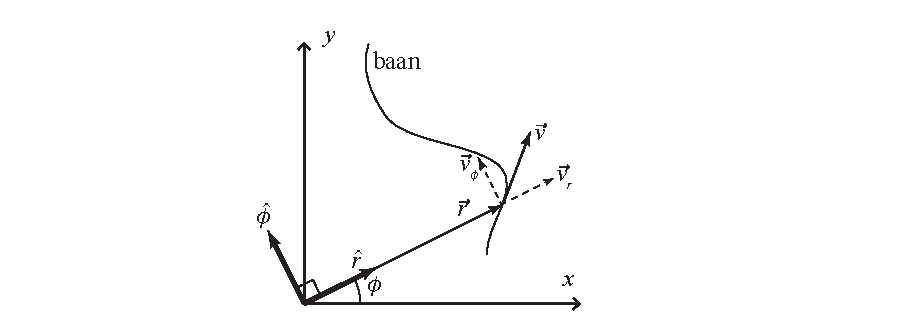
\epsfig{file=PoolCoordinaten.pdf, width=\textwidth}
\caption{{\it Positie en snelheid in poolcoordinaten.}}
\label{fig:pool}
\end{center}
\end{figure} 
Met poolcoordinaten kan je 
een positie in een 2-D vlak uitdrukken in termen van een afstand tot de oorsprong van het 
coordinatensysteem, $r$, en een hoek $\phi$, zoals aangegeven in Fig.~\ref{fig:pool}.  
\begin{equation}
\vec{r} = r \hat{r}
\end{equation}
met:
\begin{equation}
\hat{r} = (\cos\phi,\,\sin\phi)
\end{equation}
Deze laatste vector is een eenheidsvector ({\it laat zien}), die gericht staat in de radiele
richting ({\it laat zien}).  Naast een eenheidsvector in de radiele richting is het ook 
mogelijk een eenheidsvector, $\hat{\phi}$, te construeren in de azimuthale richting:
\begin{equation}
\hat{\phi} = (-\sin\phi,\,\cos\phi)
\end{equation}
Deze vector staat loodrecht op $\hat{r}$ en heeft ook lengte 1. Het blijkt dat je beweging
in het 2-D vlak met behulp van $r$, $\phi$, $\hat{r}$ en $\hat{\phi}$ volledig kan 
karakteriseren net zoals je dat kan met cartesische coordinaten. In eerste instantie kan
dit misschien iets lastiger lijken, omdat je eenheidsvectoren afhangen van de coordinaat $\phi$,
terwijl ze in cartesische coordinaten mooi constant waren. 

\begin{center}
\line(1,0){250}
\end{center}
\begin{voorbeeld} 
(i) Bewijs dat $\hat{r}$ en $\hat{\phi}$ loodrecht op elkaar staan. (ii) Bewijs dat $\hat{\phi}$ lengte~1
heeft.

{\bf Oplossing: }{\it (i) Voor het inproduct tussen twee vectoren $\vec{A}$ en $\vec{B}$ in 2-D geldt:
\begin{equation}
\vec{A}\cdot\vec{B} = A_x\,B_x+A_y\,B_y = |\vec{A}||\vec{B}|\cos\alpha
\end{equation}
Met $\alpha$ de hoek tussen de twee vectoren. Dus voor $\hat{r}$ en $\hat{\phi}$:
\begin{equation}
\hat{r}\cdot\hat{\phi} = \cos\phi\,(-\sin\phi)+\sin\phi \,\cos\phi = 0
\end{equation}
Dit impliceert dat $\alpha=\pi/2$ en dus staan de twee vectoren loodrecht op elkaar.
(ii) De lengte van een vector, $L$, is uit te rekenen door:
\begin{eqnarray}
L & = & \sqrt{\hat{\phi}\cdot\hat{\phi}} \\
& = & \sqrt{(-\sin\phi)^2+(\cos\phi)^2} \\
& = & 1
\end{eqnarray}
Q.E.D.
}
\end{voorbeeld}
\begin{center}
\line(1,0){250}
\end{center}

De snelheid van een object is zoals gewoonlijk weer gegeven door
te tijdsafgeleide te nemen van de positie. Maar nu moet je goed uitkijken, want
de tijdsafgeleide van de eenheidsvector $\hat{r}\neq\vec{0}$! Laten we eens kijken
hoe de snelheid eruit ziet:
\begin{eqnarray}
\vec{v} &=& \frac{d\vec{r}}{dt} \\
& = & \frac{dr}{dt} \hat{r} + r \frac{d\hat{r}}{dt}
\end{eqnarray} 
Laten we de tijdsafgeleide van de radiele eenheidsvector eens bekijken:
\begin{eqnarray}
\frac{d\hat{r}}{dt} & = & \frac{d}{dt}(\cos\phi,\,\sin\phi) \\
& = & \frac{d\phi}{dt}\,(-\sin\phi,\,\cos\phi) \\
& = & \frac{d\phi}{dt}\,\hat{\phi}
\end{eqnarray}
Dat is natuurlijk mooi: de tijdsafgeleide van de radiele eenheidsvector geeft
je een vector in de $\phi$ richting. We kunnen nu de snelheid schrijven als:
\begin{equation}\label{eq:vpool}
\vec{v} = \frac{dr}{dt} \hat{r} + r\frac{d\phi}{dt} \hat{\phi} = \vec{v}_{r}+\vec{v}_{\phi}
\end{equation}
De snelheid bestaat dus uit een component langs de baan van het object en
een component loodrecht daarop, in de radiele richting. Een uitdrukking als
hierboven mag je ook niet echt verbazen, want het zou natuurlijk vreemd zijn
als er een snelheid zou worden gevonden zonder $\hat{\phi}$ component. 
Daarnaast kan je zien dat de tangentiele of $\hat{\phi}$ component van de
snelheid afhangt  van de hoeksnelheid $\omega\equiv d\phi / dt$ maal
de afstand tot de oorsprong. Ook niet zo vreemd, want een kleine hoeksnelheid
met bijvoorbeeld een grote afstand kan leiden tot een grote baansnelheid, en
vice-versa.

Tenslotte kunnen we kijken hoe de versnelling van een object eruit ziet in 
poolcoordinaten. Daarvoor moeten we de tijdsafgeleide nemen van de snelheid
en dat is even stug differentieerwerk:
\begin{eqnarray}
\vec{a} & = & \frac{d\vec{v}}{dt} \\
 & = & \frac{d^2r}{dt^2}\hat{r}  + \frac{dr}{dt}\,\frac{d\hat{r}}{dt} + \frac{d}{dt}\left(r\frac{d\phi}{dt}\right)\hat{\phi} + r\frac{d\phi}{dt}\frac{d\hat{\phi}}{dt} \\ 
 & = & \left\{\frac{d^2r}{dt^2}-r\left(\frac{d\phi}{dt}\right)^2\right\}\hat{r}+\left\{2\frac{dr}{dt}\frac{d\phi}{dt}+r\frac{d^2\phi}{dt^2}\right\}\hat{\phi}\label{eq:apool} \\
 & = & \vec{a}_{r}+\vec{a}_{\phi}
 \end{eqnarray}
 In de iedere stap is gebruik gemaakt van de productregel voor differentieren, en in de laatste stap is de 
 afgeleide van $\hat{\phi}$ uitgerekend:
 \begin{equation}
 \frac{d\hat{\phi}}{dt} = -\frac{d\phi}{dt}\hat{r}
 \end{equation}
Deze vergelijking ziet er behoorlijk intimiderend uit en bevat een behoorlijke hoeveelheid 
afgeleiden en dubbele afgeleiden. En de vraag is waarom zou je nou een dergelijke vergelijking 
willen gebruiken. 

\begin{center}
\line(1,0){250}
\end{center}
\begin{voorbeeld} 
Een object beweegt over een cirkel met constante straal $r(t)=R$. De hoek $\phi(t)$ wordt gegeven door
$\phi(t) = a_0 +a_1\,t +\frac{1}{2} \, a_2\,t^2$. Bereken (i) de snelheid $\vec{v}(t)$ en (ii) de versnelling $\vec{a}(t)$.

{\bf Oplossing: }{\it (i) We hoeven alleen maar onze vergelijking voor $\phi(t)$ in te vullen in de
vergelijking voor de snelheid~\ref{eq:vpool} en ons te bedenken dat $dR/dt=0$:
\begin{eqnarray}
\vec{v} & = & \frac{dR}{dt}\hat{r} + R\frac{d\phi}{dt}\hat{\phi} \\
& = & R\left(a_1 + a_2\,t\right)\hat{\phi}
\end{eqnarray}
De snelheid heeft dus alleen een $\hat{\phi}$ component, wat je natuurlijk ook verwacht voor een baan
met constante straal. (ii) De versnelling wordt gegeven door vgl.~\ref{eq:apool}. Invullen levert:
\begin{eqnarray}
\vec{a} & = & -R\left(a_1+a_2\,t\right)^2\,\hat{r} + R\,a_2\,\hat{\phi}
\end{eqnarray}
De versnelling heeft dus wel degelijk een $\hat{r}$ component, ondanks dat de straal van de baan constant 
is! (Ga zelf na wat de eenheden van de constanten $a_0$, $a_1$ en $a_2$ moeten zijn, en controleer dat de
dimensie van het antwoord klopt.
}
\end{voorbeeld}
\begin{center}
\line(1,0){250}
\end{center}
 

\section{Eenparige cirkelbeweging}

De vergelijkingen voor beweging in poolcoordinaten kunnen uitstekend worden toegepast 
in het geval van eenparige cirkelbeweging zoals getekend in Fig.~\ref{fig:cirkel}. 
 \begin{figure}[htbp]
\begin{center}
  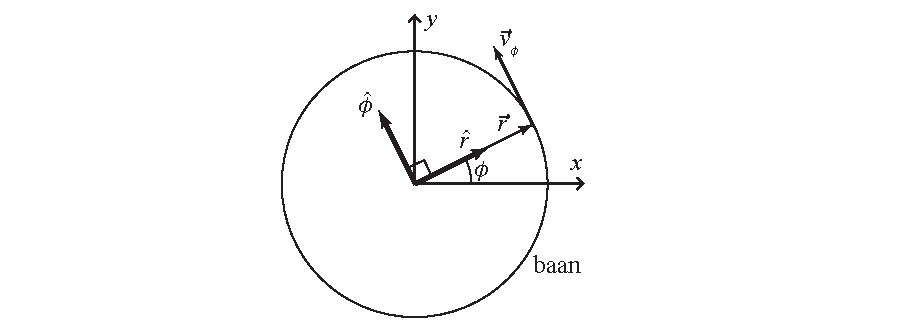
\epsfig{file=EenparigeCirkel.pdf, width=\textwidth}
\caption{{\it Eenparige cirkelbeweging.}}
\label{fig:cirkel}
\end{center}
\end{figure} 
Bij eenparige 
cirkelbeweging is er sprake van een beweging op een cirkel met constante straal en een
constante hoeksnelheid. Dus:
\begin{eqnarray}
\frac{dr}{dt} & = & 0\\
\frac{d^2r}{dt^2} & = & 0 \\
\frac{d\phi}{dt} &= & \omega = \mbox{constant} \\
\frac{d^2\phi}{dt^2} & = & 0
\end{eqnarray}
Het gevolg is dat de vergelijkingen voor snelheid en versnelling nu in poolcoordinaten er 
een stuk eenvoudiger uitzien dan in cartesische coordinaten. Voor de snelheid zoals in
vgl.~\ref{eq:vpool} geldt nu:
\begin{eqnarray}\label{eq:vpoolcir}
\vec{v} & =&  \vec{v}_{\phi} \\
             & =& \omega\,R\,\hat{\phi}
\end{eqnarray}
Hierin is de constante straal van de baan, $R$, en de hoeksnelheid $\omega$ is weer 
$d\phi / dt$. Ook de hoeksnelheid is nu constant.

De vergelijking  voor de versnelling in poolcoordinaten~\ref{eq:apool} reduceert nu tot:
\begin{eqnarray}\label{eq:apoolcir}
\vec{a} & = & -\omega^2\,R\,\hat{r}
\end{eqnarray}
En dit is een stuk eenvoudiger dan de versnelling in cartesische coordinaten. Bovendien
leer je direct uit deze vergelijking dat er een versnelling in de radiele richting nodig is om een
eenparige cirkelbeweging te laten plaatsvinden. De richting van deze versnelling is naar
het centrum van de cirkel gericht en heet de {\emph centripetale} ofwel middelpuntzoekende
versnelling. Vaak wordt er gesproken over een centrifugale of middelpuntvliedende versnelling,
maar meestal zijn het geen natuurkundigen die een dergelijke discussie voeren. Er bestaat
namelijk niet zoiets als een centrifugale versnelling: als de centripetale versnelling er niet
zou zijn dan beweeg je gewoon weer met een constante snelheid. Wat verder opmerkelijk is 
aan de eenparige cirkelbeweging, is dat een object continue een versnelling ondervindt, 
terwijl de grootte van de snelheid niet verandert.

Tenslotte kan je vgl.~\ref{eq:apoolcir} met gebruik van de vergelijking voor de snelheid~\ref{eq:vpoolcir}
herschrijven tot:
\begin{equation}
\vec{a} = -\frac{|\vec{v}|^2}{R}\hat{r}
\end{equation}
De bijbehorende centripetale kracht, $\vec{F}_C$ nodig om een object met massa $m$ in een baan met straal $R$
te houden is nu natuurlijk direct te schrijven schrijven als:
\begin{equation}\label{eq:fc_cirkel}
\vec{F}_C = -\frac{m\,|\vec{v}|^2}{R}\hat{r}
\end{equation}
De centripetale kracht is dus evenredig met $|\vec{v}|^2$ en dat betekent dat de kracht snel 
groter wordt als je snel door een bocht wil. Eveneens wordt de kracht veel groter als je een
kleine draaicirkel kiest.

\begin{center}
\line(1,0){250}
\end{center}
\begin{voorbeeld} 
Een slinger met lengte $l$ zoals getekend in Fig.~\ref{fig:cirkelvoorbeeld}~a) draait met constante
snelheid rondjes (\emph{let op: de grootte van de snelheid is constant, de richting verandert}). Bereken 
de hoek $\theta$.
 \begin{figure}[htbp]
\begin{center}
  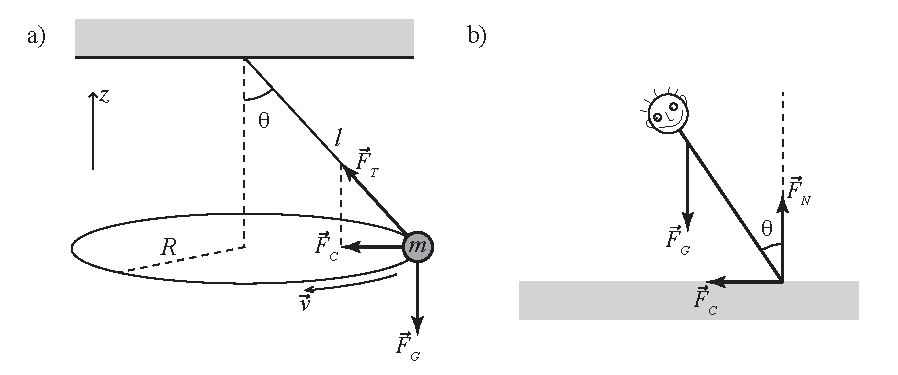
\epsfig{file=CentripetaalVoorbeeld.pdf, width=\textwidth}
\caption{{\it a) Ronddraaiende slinger. b) Colijn in de bocht.}}
\label{fig:cirkelvoorbeeld}
\end{center}
\end{figure} 

{\bf Oplossing: }{\it De eerste stap voor de oplossing van dit probleem is het maken van een tekening met alle krachten
op de massa $m$ zoals in Fig.~\ref{fig:cirkelvoorbeeld}~a) staan aangegeven.  Naast de $\hat{r}$ en $\hat{\phi}$ 
coordinaat kiezen we ook een $z$-as zoals getekend. De $z$ component van de spankracht, $\vec{F}_T$ in de slinger 
is even groot als de zwaartekracht op de massa, maar tegengesteld van richting. De massa beweegt immers met 
constante snelheid en hangt dus op constante $z$. Dus;
\begin{equation}
m\,g = |\vec{F}_T|_z = |\vec{F}_T|\cos\theta
\end{equation}
De radiele component van de spankracht zorgt levert de centripetale versnelling om de massa in de bocht te houden. De
straal $R$ van de baan is gegeven door $R=l \sin\theta$. We kunnen schrijven:
\begin{eqnarray}
|\vec{F}_C| & = & |\vec{F}_T|_r\\
\frac{m|\vec{v}|^2}{R} & = & |\vec{F}_T|\sin\theta \\
\frac{m|\vec{v}|^2}{l\sin\theta} & = & |\vec{F}_T|\sin\theta
\end{eqnarray}
Nu kunnen we listig de laatste vergelijking delen door de vorige. Op die manier raken we de spankracht 
kwijt uit onze vergelijking en krijgen we de volgende uitdrukking:
\begin{eqnarray}
\tan\theta & = & \frac{|\vec{v}|^2}{l\,\sin\theta\,g} \\
& \Downarrow & \\
\frac{\sin^2\theta}{\cos\theta} & = & \frac{|\vec{v}|^2}{l\,g}
\end{eqnarray}
De uitwijking hangt dus alleen maar af van de snelheid, de lengte van de slinger en $g$. De massa speelt geen rol voor
de uitwijking, maar uiteraard wel voor de spankracht in het touw. Reken die maar eens uit.
}
\end{voorbeeld}
\begin{center}
\line(1,0){250}
\end{center}
\begin{voorbeeld} 
Docent Colijn gaat door de bocht met snelheid $\vec{v}$ ($|\vec{v}|$ is constant) op een oppervlak met statische wrijving, 
gekarakteriseerd door wrijvingscoefficient $\mu_s$ zoals in Fig.~\ref{fig:cirkelvoorbeeld}~b). 
(i) Druk de hoek $\theta$ uit in bekende grootheden. (ii) Wat is de minimale straal $R$ van de bocht, zonder dat Colijn uitglijdt?  

{\bf Oplossing:}{\it (i) Teken alle krachten op Colijn. Uit de tekening blijkt dat de hoek $\theta$ wordt gegeven door:
\begin{eqnarray}
\tan\theta & = & \frac{|\vec{F}_C|}{|\vec{F}_N|} \\
& = & \frac{|\vec{v}|^2}{R\,g}
\end{eqnarray}
Weer onafhankelijk van de massa. Tweewielers die met dezelfde snelheid door de bocht gaan, maken altijd exact dezelfde
hoek met het wegdek. De wrijvingskracht zorgt ervoor dat hier de centripetaalkracht wordt geleverd: als je dus maar snel genoeg 
door de bocht gaat zal je uiteindelijk uitglijden. Vaak wordt een wegdek onder een zodanige hoek aangelegd dat 
de centripetaal versnelling bij een vooraf gekozen snelheid volledig wordt geleverd door de normaalkracht. Zulke bochten
zijn comfortabel, ook voor passagiers van een auto, omdat ze niet zijwaarts worden versneld. (ii) Deze discussie 
brengt ons meteen bij de tweede vraag. De minimale straal van de bocht voor een gegeven snelheid $v$ wordt gevonden 
door de centripetale kracht gelijk te stellen aan de maximale wrijvingskracht:
\begin{eqnarray}
\frac{m|\vec{v}|^2}{R} & = & \mu_s \,m\,g \\
& \Downarrow& \\
R_{min} & = & \frac{|\vec{v}|^2}{\mu_s \,g}
\end{eqnarray}
De minimale straal, $R_{min}$, neemt dus kwadratische toe met de snelheid. daarnaast zie je dat als er weinig 
wrijving is de minimale straal ook toeneemt. Als de wrijving erg klein is - denk aan het lopen op een net gepoetste 
ijsbaan - zie je dat het erg moeilijk wordt om kleine rondjes te draaien.
}
\end{voorbeeld}
\begin{center}
\line(1,0){250}
\end{center}

% \section{Centrale krachten}

\section{Wat moet ik weten en kunnen?}

Na bestuderen van dit hoofdstuk moet je weten:
\begin{itemize}
\item Hoe positie, snelheid en versnelling eruit zien in poolcoordinaten.
\item Hoe je een cirkelbeweging beschrijft.
\item Wat centripetaalkracht is.
\end{itemize}
En je moet kunnen:
\begin{itemize}
\item Rekenen met poolcoordinaten.
\item Rekenen met centripetaalkrachten.
\end{itemize}

\section{Opgaven}

\begin{enumerate}
\item Selectie Giancoli hoofdstuk 5:  46, 47, 54, 62, 64, 80, 87, 92, 93, 100, 101
\item Op een schijf die draait met constante hoeksnelheid $\omega$ bevindt zich 
een karretje met massa $m$ zoals in Fig.~\ref{fig:BalInBuis}. 
 \begin{figure}[htbp]
\begin{center}
  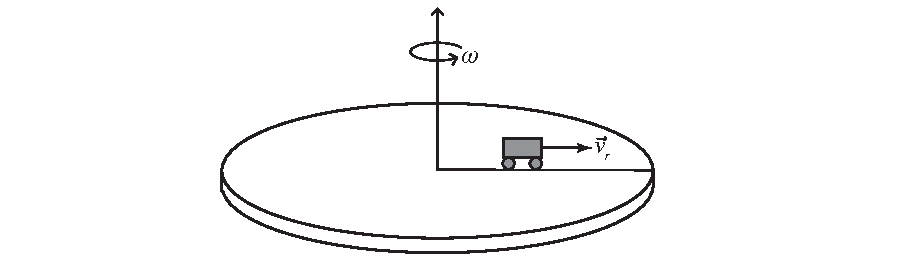
\epsfig{file=BalInBuis.pdf, width=\textwidth}
\caption{{\it Een karretje op een draaiende schijf.}}
\label{fig:BalInBuis}
\end{center}
\end{figure} 
In de radiele richting 
kan het  karretje vrij bewegen, terwijl deze in de $\phi$ richting meedraait met de schijf.
Stel een vergelijking op voor de radiele snelheid als functie van de tijd. Kan je deze
vergelijking oplossen?
\item Waarom spreken zoveel mensen van centrifugaalkrachten? Kan je dit begrijpen? 
Leg uit.
\item Een systeem zoals getekend in Fig.~\ref{fig:flyball} draait rond met hoeksnelheid
$\omega$. Massa $M$ kan vrij glijden over de draaias van het systeem. Bereken
hoek $\theta$.
 \begin{figure}[htbp]
\begin{center}
  
\epsfig{file=FlyballGovernor.pdf, width=\textwidth}
\caption{{\it Glijdende en draaiende massa's.}}
\label{fig:flyball}
\end{center}
\end{figure} 

\end{enumerate}



%%%%%%%%%%%%%%%%%%%%%%%%%%%%%%%%%%%%%%%%%%%%%%%
% BEGIN ARBEID EN ENERGIE
%%%%%%%%%%%%%%%%%%%%%%%%%%%%%%%%%%%%%%%%%%%%%%%

\chapter{Arbeid en Energie}\label{chap:energie}

In dit hoofdstuk worden arbeid en energie geintroduceerd. Deze zeer belangrijke begrippen
in de klassieke fysica zijn ook voor quantumfysica en relativiteitstheorie van levensbelang. Als
je daarom de klassieke begrippen goed kent, maak je daarmee je introductie in de moderne 
natuurkunde een stuk eenvoudiger.  Verder wordt er in dit hoofdstuk aandacht besteed aan
behoud van energie en in welke gevallen je daarmee op eenvoudige wijze ingewikkelde
problemen kan oplossen.

In Giancoli worden energie en behoud daarvan behandeld in:
\begin{itemize}
\item Hoofdstuk 7
\item Hoofdstuk 8
\end{itemize}

\section{Arbeid en Vermogen}

Arbeid is het eerste belangrijke begrip dat met energie te maken heeft, en aan de hand van
arbeid kunnen we alle vormen van energie exact definieren. In het dagelijks leven heeft het 
begrip arbeid een brede betekenis, maar de natuurkunde zou de natuurkunde niet zijn als
er niet een eenduidige definitie van het begrip arbeid was. Een hoeveelheid arbeid, $\Delta W$,
verricht door een bepaalde kracht $\vec{F}_P$, is gerelateerd aan de hoeveelheid 
verplaatsing, $\Delta x$, in de richting van die kracht:
\begin{equation} 
\Delta W = \vec{F}_P\cdot\vec{\Delta x} 
\end{equation}
De "stip" tussen de kracht en de verplaatsingsvector staat voor het inproduct zoals gedefinieerd
in paragraaf~\ref{sec:vectorcalculus}. Even voor alle duidelijkheid: arbeid is een scalaire grootheid
en gelukkig zorgt het inproduct er voor dat er aan de rechterzijde ook een scalar staat. 
 \begin{figure}[htbp]
\begin{center}
  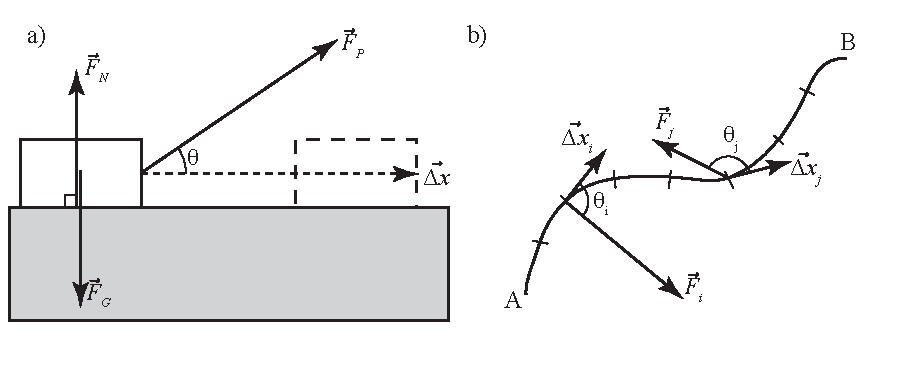
\epsfig{file=Arbeid.pdf, width=\textwidth}
\caption{{\it a) Arbeid in het geval van een constante kracht. b) Arbeid in het algemeen.}}
\label{fig:W}
\end{center}
\end{figure} 
Het inproduct kan ook worden geschreven met behulp van de hoek tussen de kracht en
de verplaatsing zoals getekend in Fig.~\ref{fig:W}~a) als:
\begin{equation}
\Delta W = |\vec{F}_P||\vec{\Delta x}|\cos\theta
\end{equation}
Hieruit zie je onmiddellijk dat de hoeveelheid arbeid alleen afhangt van de component
van de kracht in de richting van de verplaatsing. Wat je ook ziet is dat zowel de zwaartekracht
en normaalkracht in dit specifieke geval geen arbeid verrichten. Hoe wonderlijk het ook 
mag klinken, er hoeft geen arbeid te worden verricht voor verplaatsingen loodrecht op de 
richting van een kracht. Als jij bijvoorbeeld een steen aan een touw boven je hoofd rondslingert, 
verricht je geen arbeid. 

We kunnen het begrip van arbeid meer algemeen definieren voor een willekeurig pad van
A naar B en een willekeurige kracht die als functie van de positie van grootte en richting 
kan veranderen, zoals aangegeven in Fig.~\ref{fig:W}~b). Het enige dat we in dit 
geval moeten doen is het pad opknippen in kleine stukjes aangegeven met $\vec{\Delta x}_i$. 
Vervolgens kan je voor ieder klein stapje uitrekenen hoeveel arbeid de kracht moet
verrichten. Tenslotte moet je alle kleine beetjes bij elkaar optellen om de totale arbeid te
krijgen. Mathematisch kan je dit uiteraard veel korter 'zeggen':
\begin{equation}\label{eq:work_sum}
W = \sum_i \vec{F}_i \cdot \vec{\Delta x}_i = \sum_i |\vec{F}_i||\vec{\Delta x}_i|\cos\theta_i
\end{equation}
Tot nog toe niets verrassend, maar we er zit natuurlijk een onnauwkeurigheid in onze
berekening van $W$, vanwege de eindige stapgrootte $\vec{\Delta x}_i$. We kunnen
nu het aantal stappen naar oneindig laten gaan, terwijl we de stapgrootte oneindig
klein wordt. We kunnen dan de som in vgl.~\ref{eq:work_sum} vervangen door een
integraal (wellicht kennen jullie deze stap al van calculus als de definitie van een integraal):
\begin{equation}\label{eq:defwork}
W = \int_A^B \vec{F}\cdot d\vec{\ell}
\end{equation} 
In het nemen van de limiet hebben we voor alle duidelijkheid $\vec{\Delta x}_i$ vervangen
door $d\vec{\ell}$.
Voor berekenen van de arbeid moet je dus langs je willekeurige pad van A naar B telkens
het inproduct tussen de kracht en de verplaatsing uitrekenen en de resultaten voor elke infinitesimale stap bij elkaar optellen.

\begin{center}
\line(1,0){250}
\end{center}
\begin{voorbeeld} 
Sisyphus houdt ervan dag-in, dag-uit een zware zwerfkei met massa $m$ een helling 
op te duwen. De helling heeft hoogte $h$ en maakt een hoek $\theta$. Om Sisyphus
het niet al te gemakkelijk te maken heeft de helling een coefficient van kinetische
wrijving $\mu_k$.  (i) Hoeveel arbeid moet Sisyphus verzetten om zijn zwerfkei met 
constante snelheid de helling op te duwen? (ii) Bereken hoeveel arbeid elke kracht verzet.
(iii) Wat is de totale hoeveelheid arbeid door alle krachten op de steen?

{\bf Oplossing: }{\it (i) Laten we aannemen dat Sisyphus langs de helling een kracht $\vec{F}_S$ 
uitoefent zoals in Fig.~\ref{fig:sisyphus}. 
 \begin{figure}[htbp]
\begin{center}
  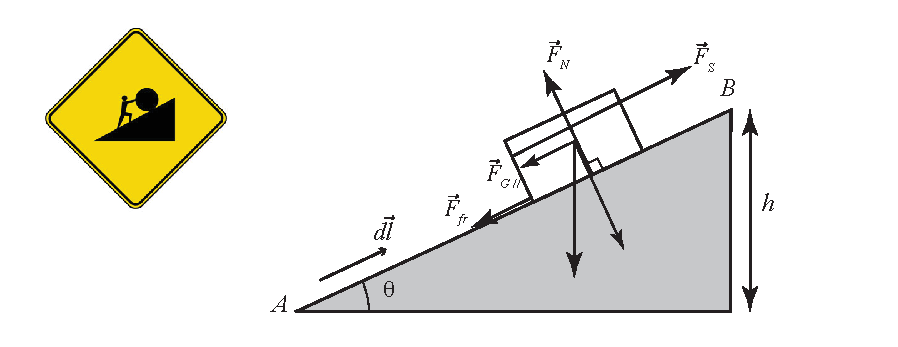
\epsfig{file=Zwerfkei.pdf, width=\textwidth}
\caption{{\it Je moet arbeid leveren om een kei een berg op te duwen.}}
\label{fig:sisyphus}
\end{center}
\end{figure} 
Deze grootte van deze kracht zal gelijk zijn aan de som van alle andere krachten
die parallel aan de helling staan, omdat we een constante snelheid aannemen, $a=0$. Dus:
\begin{eqnarray}
\vec{F}_S & = & \vec{F}_{G\,//}+\vec{F}_{fr} \\
 |\vec{F}_S|  & = & m\,g\,\sin\theta + \mu_k\,m\,g\,\cos\theta 
\end{eqnarray}
Nu we de kracht hebben die Sisyphus moet uitoefenen, kunnen we de arbeid uitrekenen door:
\begin{eqnarray}
W & = & \int_A^B \vec{F}_S \cdot d\vec{\ell} \\
     & = & \int_A^B |\vec{F}_S| |d\vec{\ell}| \\
     & = & (m\,g\,\sin\theta + m\,g\,\mu_k\,\cos\theta)\,L \\
     & = & m\,g\, (\sin\theta + \mu_k\,\cos\theta)\,\frac{h}{\sin\theta} \\
     & = & m\,g\,h + \frac{\mu_k \,m\,g\, h}{\tan\theta}
\end{eqnarray} 
Voor de tweede stap hebben we gebruikt dat het integratiepad langs de helling loopt. De
hoek tussen de kracht $\vec{F}_S$ en $d\vec{\ell}$ is dan $0^{\circ}$. Verder hebben we gebruikt
dat de lengte van de helling is gegeven door $h / \sin\theta$. Je ziet dat de arbeid die
moet worden geleverd bestaat uit een component tegen de zwaartekracht in en een component
tegen de wrijving. (ii) De arbeid die de zwaartekracht heeft verzet is gelijk aan $W_G=-m\,g\,h$ en
de arbeid die de wrijving heeft geleverd is $W_{fr}=-\mu_k \, h / \tan\theta$. In beide gevallen
is de netto verplaatsing tegen de richting van de kracht in. (iii) De totale arbeid van alle
krachten samen is $W=0$, omdat de zwerfkei met constante snelheid beweegt en de totale
kracht dus gelijk is aan $\vec{F}_{tot}=\vec{0}$
}
\end{voorbeeld}
\begin{center}
\line(1,0){250}
\end{center}

Tenslotte is het nog van belang te kijken naar de snelheid waarmee arbeid wordt
geleverd. Als je een zwerfkei de trap op draagt ligt de hoeveelheid arbeid die  je moet
leveren vast, maar je kan ervoor kiezen om langzaam of snel het pad af te leggen. 
Vermogen, $P$, is gedefinieerd als:
\begin{equation}\label{eq:vermogen1}
P = \frac{dW}{dt} 
\end{equation}
We kunnen nu het vermogen relateren aan kracht en snelheid door het volgende 
te schrijven:
\begin{eqnarray}
dW & =  &  \vec{F}\cdot d\vec{\ell} \\
       & \Downarrow & \\
P=\frac{dW}{dt}   & = & \frac{d \vec{F}\cdot d\vec{\ell}}{dt}\\
      & = & \vec{F}\cdot\vec{v}\label{eq:vermogen2}
\end{eqnarray}
Hoewel bovenstaande formule ook wel wiskundig netjes kan worden afgeleid, geldt
dus dat het vermogen gelijk is aan het inproduct van snelheid en kracht.    

\section{Kinetische energie}

Laten we de uitdrukking die we voor de arbeid hebben gevonden eens onder de loep 
nemen. We kunnen de $2^e$ wet van Newton gebruiken om de kracht die voorkomt
in de vergelijking expliciet uit te schrijven:
\begin{eqnarray}
W & = & \int_A^B \vec{F}\cdot d\vec{\ell} \\
    &  = & m\,\int_A^B \frac{d\vec{v}}{dt}\cdot d\vec{\ell} \\
    & = & m\,\int_A^B \frac{d\vec{v}}{dt}\cdot\frac{d\vec{r}}{dt}\,dt \\
    & = & m\,\int_A^B \frac{d\vec{v}}{dt}\cdot\vec{v} \, dt \label{eq:kintmp}
\end{eqnarray}
Let er op dat we het hier hebben over de totale of netto kracht op een object.
We hebben nu een uitdrukking voor de arbeid die zowel de snelheid als de $1^e$ afgeleide 
van de snelheid naar de tijd bevat en die er bovendien tamelijk onsmakelijk uitziet. Maar
laten we nu eerst eens de productregel in gedachten roepen voor differentieren van 
een functie $h(t)=f(t)\,g(t)$. Voor de afgeleide van $f(t)$ naar de tijd krijgen we:
\begin{equation}
\frac{dh}{dt} = f \, \frac{dg}{dt} + \frac{df}{dt}\,g
\end{equation}
Laten we nu een functie $h$ nemen die er uit ziet als:
\begin{equation}
h(t) = f(t) \, f(t)
\end{equation}
Dan geldt voor de afgeleide van $h(t)$ naar de tijd:
\begin{equation}
\frac{dh}{dt} = f\,\frac{df}{dt} + \frac{df}{dt}\,f = 2\,f\frac{df}{dt}
\end{equation}
Dit resultaat gaan we gebruiken om  vgl.~\ref{eq:kintmp} tot de orde te roepen. We kunnen
de laatste regel van vgl.~\ref{eq:kintmp} nu herschrijven als:
\begin{equation}
W = \frac{1}{2}\,m\,\int_A^B\frac{d}{dt} \left( \vec{v} \cdot \vec{v} \right) \,dt
\end{equation}
Deze integraal is uitermate simpel. Je moet namelijk de afgeleide van een functie naar
de tijd integreren over de tijd. Dat geeft niets anders dan de functie zelf:
\begin{equation}
W = \frac{1}{2} \,m\,\left[|\vec{v}|^2\right]_A^B = 
\frac{1}{2}\,m\,|\vec{v}_B|^2 - \frac{1}{2}\,m\,|\vec{v}_A|^2
\end{equation} 
In deze vergelijking stellen de termen aan de rechterkant van de vergelijking de jullie 
welbekende bewegings- of kinetische energie. Dus de netto arbeid op een object leidt tot
een verandering van de kinetische energie, $\Delta K$,  van een object:
\begin{equation}
W = K_2 - K_1 = \Delta K
\end{equation}

\begin{center}
\line(1,0){250}
\end{center}
\begin{voorbeeld} 
Je duwt met kracht $\vec{F}_D$ over een afstand $L$ tegen een object met massa $m$ dat op een
horizontale vloer staat, zonder wrijving. (i) Wat is de kinetische energie na afstand $L$, als de
beginsnelheid nul is? (ii) Wat is de snelheid na afstand $L$?

{\bf Oplossing: }{\it (i) De arbeid die je hebt verricht is:
\begin{equation}
W=\int \vec{F}\cdot\vec{d l} = |\vec{F}_D|\,L= K
\end{equation}
We hebben er gebruik van gemaakt dat het object op een horizontale vloer staat. De zwaartekracht
en de normaalkracht staan loodrecht op de afgelegde weg $d\vec{\ell}$ en leveren dus geen
bijdrage aan de arbeid. 

(ii) De snelheid na afstand $L$ kunnen we oplossen door $K$ gelijk te stellen aan de expliciete
uitdrukking voor de kinetische energie:
\begin{eqnarray}
|\vec{F}_D|\, L & = & \frac{1}{2}\,m\,|\vec{v}|^2 \\
& \Downarrow & \\
|\vec{v}| &  = & \sqrt{\frac{2\,|\vec{F}_D|\,L}{m}}
\end{eqnarray}
Dat is een mooie uitdrukking. Maar wacht nou eens even: dit is een eenparig versnelde 
beweging en daar hadden we in paragraaf~\ref{sec:eenparig} al een uitdrukking gevonden
voor snelheid als functie van de tijd. Wanneer de startsnelheid $\vec{0}$ is geldt:
\begin{equation}\label{ex:attmp}
\vec{v}(t) = \vec{a}\,t
\end{equation}
De versnelling $\vec{a}$ is gelijk aan $\vec{F}_D/m$. Nu moeten we alleen nog even de
tijd uitrekenen die het object over afstand $L$ doet. Dat kunnen we doen door gebruik
te maken van:
\begin{eqnarray}
\vec{r}(t) & = & \frac{1}{2}\,\vec{a}\,t^2 \\
 & \Downarrow & \\
 t & = & \sqrt{\frac{2\,L\,m}{|\vec{F}_D|}}
\end{eqnarray}
Invullen in vgl.~\ref{ex:attmp} - ik zeg doen! - geeft dezelfde uitdrukking voor de eindsnelheid
als die we met de arbeid-energie analyse hebben gevonden. Dit is van groot belang, omdat
we proberen een met zichzelf consistente natuurkunde op te bouwen. Aan de andere kant
is het misschien ook niet al te verrassend dat we hetzelfde antwoord vinden, aangezien
we in beide gevallen zijn uitgegaan van de wetten van Newton (welke?) om tot ons antwoord te
komen.
}
\end{voorbeeld}
\begin{center}
\line(1,0){250}
\end{center}

\section{Conservatieve krachten}

Het blijkt er handig om krachten die we tegenkomen in twee categorie\"{e}n in te delen: 
conservatieve en niet-conservatieve krachten. {\it Een kracht heet conservatief wanneer de arbeid gedaan door
deze kracht door het bewegen van een object van een plek naar een andere onafhankelijk
is van het gekozen pad}. Alle andere krachten zijn niet-conservatief. Een conservatieve 
kracht moet kan slechts afhangen van de positie en niet van andere grootheden als snelheid 
en tijd. 

Laten we eens kijken naar een voorbeeld met zwaartekracht. Stel dat we een massa $m$ langs
een willekeurig pad van $A$ naar $B$ willen brengen waarbij punt $B$ en punt $A$ een
hoogteverschil $h$ hebben. 
 \begin{figure}[htbp]
\begin{center}
  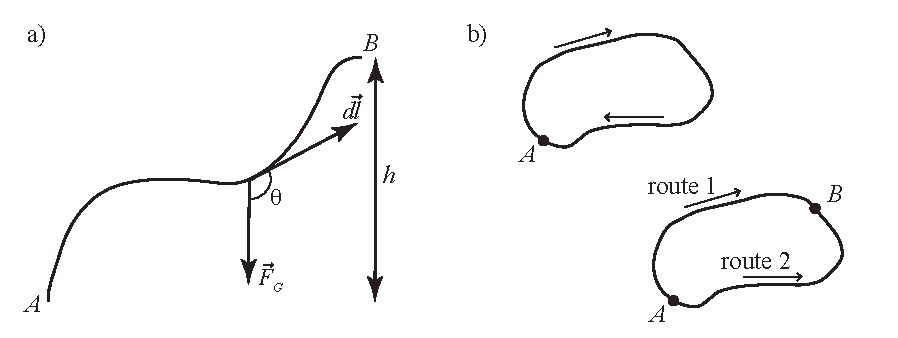
\epsfig{file=Conservatief.pdf, width=\textwidth}
\caption{{\it a) Arbeid door de zwaartekracht. b) Arbeid langs een gesloten pad.}}
\label{fig:conservatief}
\end{center}
\end{figure} 
Dan kunnen we zoals in Fig.~\ref{fig:conservatief} een willekeurig
pad kiezen van $A$ naar $B$ en de arbeid die wordt verricht door de zwaartekracht schrijven
als:
\begin{equation}\label{eq:cons}
W_G = \int_A^B \vec{F}_G\,\cdot\,d\vec{\ell}
\end{equation}
Nu lijkt deze vergelijking op het eerste gezicht duidelijk afhankelijk van het gekozen pad:
immers er komt een pad gedefinieerd door $d\vec{\ell}=(dx,\,dy,\,dz)$ in voor en niets zegt 
mij hoe ik dat pad moet kiezen. Als de zwaartekracht een conservatieve kracht is, zouden 
we moeten kunnen laten zien dat het pad niet uitmaakt. En dat is dit geval eenvoudig: de 
zwaartekracht wordt namelijk gegeven door $\vec{F}_G=(0,\,0,\,-m\,g)$, waardoor  het
inproduct in vgl .~\ref{eq:cons} kan worden uitgewerkt en de vergelijking reduceert tot:
\begin{eqnarray}
W_G & = & \int_A^B (-m\,g)\,dz \\
          & = & -m\,g\,h
\end{eqnarray}
Let op het minteken van de arbeid: de arbeid die door de zwaartekracht is uitgeoefend 
is negatief omdat we punt $B$ boven punt $A$ hebben gekozen. De externe arbeid die is 
uitgeoefend om het object te tillen is uiteraard positief. Het is altijd lastig om bij gedane
arbeid het teken goed te krijgen en te houden.

\begin{center}
\line(1,0){250}
\end{center}
\begin{voorbeeld} \label{ex:cons1}
Een alternatieve definitie van een conservatieve kracht stelt: {\it"Een conservatieve kracht is een 
kracht waarvoor de arbeid rond een willekeurig gesloten pad nul is"}. Bewijs dat dit equivalent
is met de bovenstaande definitie van een conservatieve kracht.

{\bf Oplossing: }{\it Voor dit bewijs rekenen we de arbeid uit langs gesloten pad zoals aangegeven
in Fig.~\ref{fig:conservatief}~b). Dus:
\begin{equation}
W=\int_A^A \vec{F}\cdot\vec{d l}
\end{equation}
Volgens onze alternatieve definitie van een conservatieve kracht zou hier dus nul uit moeten 
komen.  Nu moeten we kijken of er volgens onze originele definitie van een conservatieve kracht 
ook nul uitkomt.

We bekijken daarvoor hetzelfde pad, maar nu opgedeeld in twee etappes: een van $A\rightarrow B$ via 
route~1 en een van $B\rightarrow A$ via route~2. Voor de arbeid van $B\rightarrow A$ langs route~2  
geldt:
\begin{equation}
W_{B\rightarrow A}(\mbox{route~2}) = -W_{A\rightarrow B}(\mbox{route~2})
\end{equation}
Dit volgt direct uit de definitie van de arbeid: als je een pad in tegengestelde richting loopt, dan
verandert $\vec{d l}$ van teken en dus ook de arbeid. Onze originele definitie van een
conservatieve kracht vertelt ons dat de arbeid onafhankelijk is van het gekozen pad, dus:
\begin{equation}
W_{A\rightarrow B}(\mbox{route~1})= W_{A\rightarrow B}(\mbox{route~2})
\end{equation}
Nu kunnen we de arbeid langs het gesloten pad uitrekenen:
\begin{eqnarray}
W_{A\rightarrow A} & = & W_{A\rightarrow B}(\mbox{route 1}) + W_{B\rightarrow A}(\mbox{route~2}) \\
                                   &= & W_{A\rightarrow B}(\mbox{route 1})  - W_{A\rightarrow B}(\mbox{route~2}) \\
                                   & = & W_{A\rightarrow B}(\mbox{route 1})  - W_{A\rightarrow B}(\mbox{route~1}) \\
                                   & = & 0
\end{eqnarray}
Beide definities van conservatieve kracht zijn dus equivalent.
}
\end{voorbeeld}
\begin{center}
\line(1,0){250}
\end{center}
De definitie van een conservatieve kracht zoals in voorbeeld~\ref{ex:cons1} benadrukt
een belangrijk aspect van conservatieve krachten. De arbeid die door een conservatieve
kracht wordt gedaan is herbruikbaar: langs een gesloten pad worden alle stukken met
positieve arbeid gecompenseerd door stukken waar de arbeid negatief is. In het geval
van de zwaartekracht moet jij arbeid uitoefenen als je iets omhoog beweegt, die je kan
terugwinnen door hetzelfde object weer naar beneden te laten gaan. Vandaar ook de
naam 'conservatieve kracht', wat niets met de politieke voorkeur van een kracht te maken
heeft maar wel met het feit dat er iets 'behoudends' aan is.

Belangrijke voorbeelden van conservatieve krachten zijn de zwaartekracht, elektrische krachten,
en krachten uitgeoefend door veren en elastieken (die we later tegen gaan komen). 
Wrijvingskrachten daarentegen zijn niet-conservatief. Dat voel je natuurlijk al wel aan, aangezien
bij bijvoorbeeld het verschuiven van een zware bank in je kamer, het er wel degelijk toe doet
hoe je va $A$ naar $B$ gaat. Een langere weg betekent dat er meer arbeid moet worden gedaan, 
wat niet zo gek is voor een kracht die altijd tegengesteld staat aan de richting waarin je een
object beweegt. Andere voorbeelden van niet-conservatieve krachten zijn bijvoorbeeld
luchtwrijving en voortstuwing door raketten, motoren of mensen. 

\begin{center}
\line(1,0){250}
\end{center}
\begin{voorbeeld} \label{ex:veer1}
De kracht die een veer uitoefent als deze wordt uitgerekt of ingedrukt, wordt gegeven door 
de wet van Hooke. Deze vertelt dat de veerkracht, $F_V$, als functie van uitrekking of compressie 
wordt gegeven door:
\begin{equation}
F_V = -k\,(x -x_0)
\end{equation}
Hierbij is $k$ de veerconstante, $x-x_0$ de uitrekking of compressie, met $x_0$ de evenwichtspositie. Voor 
het gemak gaan we eens in 1-D iets uitrekenen, omdat de veren in dit college maar in 1~richting zullen worden 
ingedrukt. Bewijs dat de veerkracht conservatief is.

{\bf Oplossing: }{\it Om te bewijzen dat de veerkracht conservatief is, moeten we de arbeid van het uitrekken of indrukken
van willekeurige positie $x_A$ naar $x_B$. Dus:
\begin{eqnarray}
W & =  & \int_{x_A}^{x_B} F_V \, dx  \\
    & =  & -\frac{1}{2}\,k\,((x_B-x_0)^2 - (x_A-x_0)^2)
\end{eqnarray}
De arbeid hangt alleen af van het begin en eindpunt, en is niet afhankelijk van het gekozen pad. De 
veerkracht is dus conservatief.
}
\end{voorbeeld}
\begin{center}
\line(1,0){250}
\end{center}

\section{Potentiele energie}

In de vorige paragraaf hebben we de arbeid die een conservatieve kracht uitoefent bekeken en
gezien dat deze arbeid onafhankelijk is van het gekozen pad van $A\rightarrow B$ en alleen
afhangt van de coordinaten van het eind- en beginpunt van ons pad. We kunnen nu voor 
een conservatieve kracht een nieuwe grootheid definieren die we potentiele energie $U$ noemen.
Verschillen in potentiele energie zijn gedefinieerd als:
\begin{equation}
\Delta U = U_2 - U_1 \equiv -\int_1^2\vec{F}\cdot d\vec{\ell} 
\end{equation}
Een dergelijk verschil in potentiele energie behorend bij een conservatieve kracht geeft aan wat
voor potentie die kracht heeft om arbeid te verrichten. Let op dat potentiele energie alleen betekenis heeft
als je te maken hebt met een conservatieve kracht: voor een niet conservatieve kracht zoals wrijving hangt 
de arbeid af van het gekozen pad, en is $\Delta U$ niet eenduidig.

Als je bijvoorbeeld een zwerfkei met massa $m$ een afstand $h$ van de grond krijgt, dan
heeft deze steen een potentiele energie van $U = m\,g\,h$. Dit is de hoeveelheid arbeid die
jij - of Sisyphus - moet leveren om de zwerfkei op te tillen. Wanneer je de steen laat vallen wordt 
er weer precies een hoeveelheid arbeid $W=m\,g\,h$ geleverd door de zwaartekracht (potentiele
energie wordt omgezet in bewegingsenergie).  Nog even voor alle duidelijkheid. als je spreekt
over potentiele energie, bedoel je de potentiele energie die een object heeft in de aanwezigheid
van een bepaalde conservatieve kracht.

Nu is het vaak zo dat niet de kracht zelf, maar de potentiele energie als functie van positie
wordt gegeven. Dan kan je je afvragen of je de relatie kan vinden tussen die potentiele energie
en de bijbehorende kracht. Het antwoord is ja. Als we eerst een in 1-D kijken naar de uitdrukking
voor de potentiele energie, dan kunnen we stellen:
\begin{equation}
U(x) = -\int F(x)\,dx + C
\end{equation}
Als we nu kiezen:
\begin{equation}
F(x) = -\frac{dU(x)}{dx}
\end{equation}
Hieruit zie je dat de afgeleide van de potentiele energie naar de positie inderdaad precies de bijbehorende
kracht voorstelt. Als je een potentiele energie hebt die snel verandert als functie van de plaats is de 
kracht groot en vice-versa. Het beste kan je potentiele energie voorstellen als een heuvel met steile en minder steile
hellingen, waarbij de kracht die je moet leveren om de heuvel te beklimmen het grootst
is waar de helling het steilst is. De relatie tussen potentiele energie en kracht klopt dus met je intuitie.

Om de boel compleet te maken: voor een potentiele energie die afhangt van $(x,\,y,\,z)$ is de relatie 
tussen kracht en potentiele energie gegeven door de 3-D versie van een afgeleide:
\begin{equation}
\vec{F} = -\ihat \frac{\partial U}{\partial x} -\jhat \frac{\partial U}{\partial y} -\khat \frac{\partial U}{\partial z} 
\end{equation}
De partiele afgeleide, $\partial /\partial x$, staat voor de afgeleide naar $x$ met $y$ en $z$ constant.
In volgende vakken zullen jullie deze 3-D afgeleide nog vaak tegenkomen. Hij heet de gradient, $\vec{\nabla}$, en 
met de gradient kan de bovenstaande afgeleide worden geschreven als:
\begin{equation}
\vec{F} = -\vec{\nabla} U
\end{equation}

\section{Behoud van energie}

We hebben in de voorafgaande paragrafen twee vormen van energie ontmoet: kinetische
energie
en voor conservatieve krachten potentiele energie. Beide vormen van energie zijn gerelateerd
aan het begrip arbeid dat we in de eerste paragraaf van dit hoofdstuk zijn tegengekomen.
Door het combineren van kinetische en potentiele energie in conservatieve systemen, d.w.z 
systemen waar alleen conservatieve krachten arbeid verzetten, komen we op een van de 
belangrijkste behoudswetten in de klassieke natuurkunde: namelijk behoud van mechanische
energie. Als we 
kijken naar de som van de verandering van kinetische- en potentiele energie, dan
krijgen we:
\begin{eqnarray}
\Delta~K + \Delta~U & = & W_{netto}-W_{netto} \\
                                     & = & 0 \\
                                     & \Downarrow & \\
\frac{1}{2}\,m\,|\vec{v}_1|^2 + U_1 & = & \frac{1}{2}\,m\,|\vec{v}_2|^2+U_2
\end{eqnarray}
In het geval er alleen conservatieve krachten werken, is de som van kinetische energie
en potentiele energie, ofwel de totale energie $E_{tot}$ constant:
\begin{equation}
E_{tot} = K + U
\end{equation}

\begin{center}
\line(1,0){250}
\end{center}
\begin{voorbeeld} 
Bewijs dat energie behouden is door het expliciet berekenen van de tijdsafgeleide van de totale energie. (Doe maar in 1-D)

{\bf Oplossing: }{\it Als de totale energie behouden is, moet dus gelden:
\begin{equation}
\frac{dE_{tot}}{dt} = 0
\end{equation}
We kunnen in 1-D schrijven:
\begin{eqnarray}
\frac{dE_{tot}}{dt} & = & \frac{d}{dt}\left(\frac{1}{2}\,m\,v_x^2+U(x)\right) \\
                                & = & m\,v_x\,\frac{d v_x}{dt} + \frac{dU}{dt} \\
                                & = & m\,v_x\,a_x + \frac{dx}{dt}\frac{dU}{dx} \\
                                & = & v_x\,\left(m\,a_x - F_x\right) \\
                                & = & 0
\end{eqnarray}
We hebben gebruikt dat $F_x=-dU/dx$ en in de laatste stap hebben we simpelweg
de $2^e$ wet van Newton gebruikt. Het concept van energiebehoud dat we dus in deze
paragraaf hebben geintroduceerd, volgt in feite direct uit de wetten van Newton. Klassieke
mechanica zit wat dat betreft natuurlijk mooi consistent in elkaar.
} 
\end{voorbeeld}
\begin{center}
\line(1,0){250}
\end{center}

Als er naast conservatieve krachten ook nog niet-conservatieve krachten zoals
wrijving in het spel zijn, dan neemt de hoeveelheid mechanische energie in het systeem af als 
functie van de tijd. Een deel, en meestal alle energie wordt dan uiteindelijk gedissipeerd in
de vorm van warmte. Maar denk er wel om dat de totale energie
nog steeds behouden is: de mechanische energie wordt alleen omgezet in een vorm die
niet meer mechanisch van aard is. We kunnen de wet van behoud van mechanische
energie dan ook eenvoudig algemeen geldig maken, door er een extra term aan toe te voegen:
\begin{equation}
\Delta~K+\Delta~U +\Delta~E_{rest} = 0
\end{equation}
De term $\Delta~E_{rest}$ bevat alle vormen van energie die niet mechanisch van aard zijn.
Voor zover we weten is de wet van behoud van totale energie universeel geldig in de natuurkunde.
Er zijn tot op vandaag geen processen gevonden die de wet van behoud van energie schenden. 
Dat maakt deze wet ook tot een enorm krachtig gereedschap voor het analyseren van 
problemen. Zeker als er alleen conservatieve krachten in het spel zijn, is het oplossen
van problemen vaak een stuk eenvoudiger met behoud van energie, dan met de $2^e$ wet
van Newton, hoewel de resultaten natuurlijk hetzelfde moeten zijn.

\begin{center}
\line(1,0){250}
\end{center}
\begin{voorbeeld} 
Een slinger met lengte $l$ en massa $m$ staat op $t=0$ stil met uitwijking $\theta(t=0)=\theta_0$ zoals
in Fig.~\ref{fig:energiebehoud1}~a). Wat is de snelheid van de de massa bij uitwijking $\theta$?
 \begin{figure}[htbp]
\begin{center}
  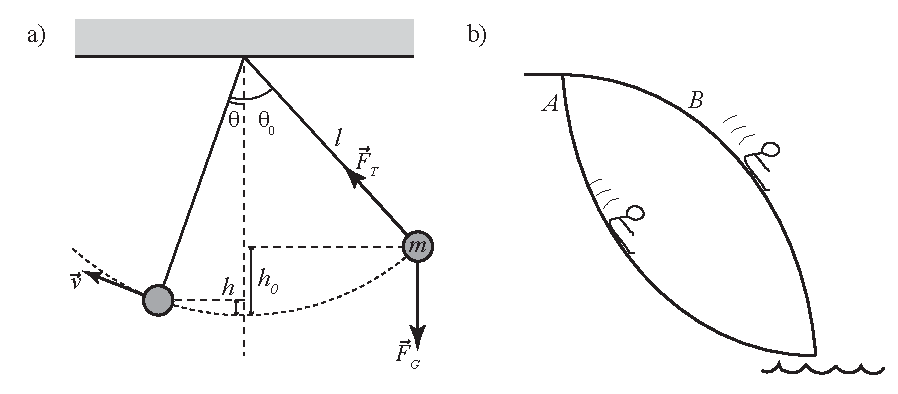
\epsfig{file=EnergiebehoudVoorbeeld.pdf, width=\textwidth}
\caption{{\it a) Slinger. b) Glijbaan}}
\label{fig:energiebehoud1}
\end{center}
\end{figure} 

{\bf Oplossing: }{\it Laten we beginnen te kijken naar de krachten die voor de slinger relevant zijn. Je
hebt de zwaartekracht, $\vec{F}_G$, op de massa en de spankracht, $\vec{F}_T$ in het touw. De zwaartekracht
is conservatief en de spankracht niet, maar toch geldt behoud van energie, omdat de spankracht geen
arbeid verricht. De spankracht staat namelijk altijd loodrecht op de bewegingsrichting van de massa.
Omdat alleen de zwaartekracht arbeid verricht kunnen we dus concluderen dat:
\begin{equation}
E = T+U = \mbox{constant}
\end{equation}
Bij het loslaten van de slinger is de snelheid $\vec{v}(t=0)=\vec{0}$ dus de massa heeft alleen potentiele
energie. Voor het uitrekenen van de potentiele energie kiezen we als de positie van de massa
voor $\theta=0$ als nulpunt. Dus voor $\theta=\theta_0$ geldt voor de potentiele energie:
\begin{equation}
U(\theta=\theta_0) = m\,g\,l\,(1-\cos\theta_0)
\end{equation}
Aangezien energie behouden is kunnen we nu de grootte van de snelheid voor een willekeurige hoek 
$\theta$ uitrekenen, door energiebehoud te gebruiken:
\begin{eqnarray}
E(\theta_0) & = & E(\theta) \\
m\,g\,l\,(1-\cos\theta_0)  & = & \frac{1}{2}\,m\,|\vec{v}|^2 + m\,g\,l\,(1-\cos\theta)  \\
  & \Downarrow & \\
|\vec{v}| &= &\sqrt{2\,g\,l\,(\cos\theta-\cos\theta_0)}  
\end{eqnarray}
Je ziet dat de snelheid onafhankelijk is van de massa en alleen afhangt van $l$, $g$ en de de beide hoeken.
Verder zie je dat je alleen de grootte van de snelheid op deze manier hebt berekend. In het geval van een
slinger kan de massa zowel met de klok mee als tegen de klok in hoek $\theta$ passeren.
} 
\end{voorbeeld}

\begin{center}
\line(1,0){250}
\end{center}

\begin{voorbeeld} 
In het zwembad zijn twee glijbanen  $A$ en $B$ zoals getekend in 
Fig.~\ref{fig:energiebehoud1}~b). De glijbanen zijn even lang en je kan zonder
wrijving naar beneden glijden. (i) Wat is de eindsnelheid die je hebt aan de bodem van 
beide glijbanen? (ii) Bij welke glijbaan bent je het eerst beneden?

{\bf Oplossing: }{\it (i) In beide gevallen is er een zelfde hoeveelheid gravitationele potentiele energie
veranderd in kinetische energie, terwijl de normaalkracht op de zwemmer geen arbeid heeft verricht. De
eindsnelheid van beide zwemmers is gelijk. (ii) Glijbaan $A$ ligt in zijn geheel onder glijbaan $B$. Op glijbaan
$A$ wordt er eerder potentiele energie omgezet in kinetische energie, en heb je dus gemiddeld een hogere
snelheid.} 
\end{voorbeeld}


\begin{center}
\line(1,0){250}
\end{center}


\begin{voorbeeld} \label{ex:achtbaan}

Een karretje glijdt zonder wrijving vanaf hoogte $h$ in een looping met straal $R$. Bij het
loslaten op $t=0$ is de snelheid van het karretje $\vec{v}(t=0)=\vec{0}$. (i) Wat is de minimale hoogte $h=h_{min}$ zodat het karretje (met docent Colijn) door de looping heen komt zonder uit
de baan te vallen (zie punt\,2 in Fig.~\ref{fig:achtbaan})? (ii) Druk de normaalkracht in punt\,1 
uit in termen van $h$ en $R$. (iii) Hoe groot is de kracht die je ondervindt op punt~1 als je op
de hoogte gevonden bij (i) begint?
 \begin{figure}[htbp]
\begin{center}
  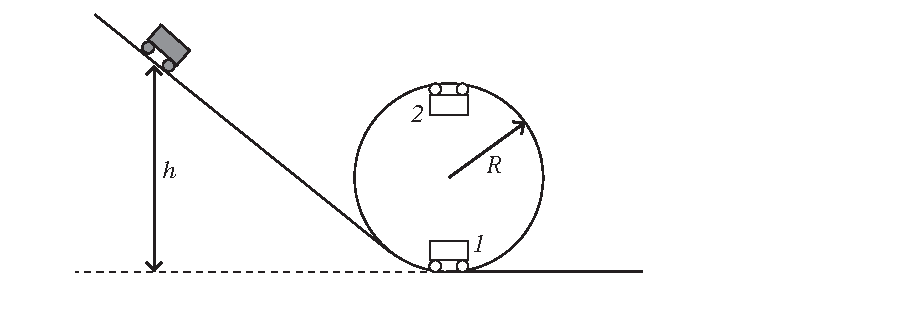
\epsfig{file=Achtbaan.pdf, width=\textwidth}
\caption{{\it Achtbaan}}
\label{fig:achtbaan}
\end{center}
\end{figure} 

{\bf Oplossing: }{\it (i) We moeten gebruik maken van energiebehoud en van hetgeen we
weten over een cirkelbeweging. Als we een krachtenanalyse maken in het punt\,2  
(teken de krachten zelf) dan zie je dat:
\begin{equation}
\vec{F}_G+\vec{F}_N = \vec{F}_C
\end{equation}
Ofwel de som van de zwaartekracht en de normaalkracht moet gelijk zijn aan de centripetaalkracht
die hoort bij het door de looping gaan. Maar de vraag is te kijken naar het geval waarbij 
het karretje net in de looping blijft: dus waarvoor geldt $\vec{F}_N = \vec{0}$. In dat geval geldt:
\begin{eqnarray}
m\,g & = & \frac{m\,|\vec{v}|^2}{R} \\
& \Downarrow & \\
|\vec{v}| & =  & \sqrt{g \, R}
\end{eqnarray}

Nu kunnen we gebruik maken van de wet van behoud van energie om te kijken wat de minimale hoogte is waarbij deze snelheid nog wordt gehaald:
\begin{eqnarray}
E(t=0)& = & E(\mbox{{\it punt 2}}) \\
m\,g\,h_{min} & = & \frac{1}{2}m\,|\vec{v}|^2 + 2\,m\,g\,R \\
& \Downarrow & \\
h_{min} & = & \frac{5}{2} R
\end{eqnarray}
Dus als je een object door een looping laat glijden met straal $R$, moet je tenminste 
vanaf een hoogte van $2.5\times$ komen om door het hoogste punt van de looping
te komen.

(ii) De normaalkracht die op je wordt uitgeoefend beneden in de looping op punt\,1 is 
de som van de centripetaalkracht en de normaalkracht ten gevolge van de zwaartekracht:
\begin{eqnarray}
\vec{F}_N & = & -\vec{F}_G +\vec{F}_C \\
& = & \left(m\,g + \frac{m\,|\vec{v}|^2}{R}\right)\khat
\end{eqnarray}
Verder weten we de snelheid in punt\,1uit energiebehoud:
\begin{eqnarray}
m\,g\,h & = & \frac{1}{2}m\,|\vec{v}|^2\\
&\Downarrow&\\
|\vec{v}| & = & \sqrt{2\,g\,h}
\end{eqnarray}
Invullen in de eerste vergelijking levert:
\begin{equation}\label{eq:exloop}
\vec{F}_N = m\,g\left(1 + \frac{2\,h}{R}\right) 
\end{equation}
Dus je 'gewicht' neemt toe als je door de bocht gaat. Dit weten jullie natuurlijk allang.

(iii) Als je de looping net haalt dan gold $h=\frac{5}{2}R$ en dit kunnen we invullen
in vgl.~\ref{eq:exloop} en dan krijgen we op punt\,1 in de looping:
\begin{equation}
\vec{F}_N  = 6\,m\,g\,\khat
\end{equation}
Je bent dan dus $6\times$ zo zwaar als normaal!
}
\end{voorbeeld}

\begin{center}
\line(1,0){250}
\end{center}

\section{Wat moet ik weten en kunnen?}

Als je dit hoofdstuk hebt bestudeerd moet je weten:
\begin{itemize}
\item Wat is arbeid, kinetische- en potentiele energie.
\item Wat is een conservatieve kracht? Wat zijn voorbeelden van dergelijke krachten?
\item Wat is een niet-conservatieve kracht? Wat zijn voorbeelden van dergelijke krachten?
\item Behoud van energie in het algemeen.
\item Behoud van mechanische energie, als er alleen conservatieve krachten werken.
\end{itemize}
En je moet kunnen:
\begin{itemize}
\item Arbeid uitrekenen.
\item Kinetische en potentiele energie uitrekenen.
\item Behoud van energie gebruiken om problemen op te lossen.
\end{itemize}

\section{Opdrachten}

\begin{enumerate}
\item Giancoli hoofdstuk 7: 1, 6, 11, (16 - 25), 33, 35, 42, 43, 45, 46, 57, 60, 61, 63, 64, 68, 75, 79, 86, 90, 91 
\item Giancoli hoofdstuk 8: 7, 8, 9, 17, 21, 22, 23, 28, 36, 42, 83, 84, 85, 86, 87, 92 
\item Wat is de eenheid van arbeid? En van kinetische en potentiele energie?
\item Leg uit waarom wrijving geen conservatieve kracht kan zijn.
\item Leg uit waarom een conservatieve kracht niet kan afhangen van snelheid.
\item Kijk nog eens naar voorbeeld~\ref{ex:achtbaan}. Wat gebeurt er met $h_{min}$ als
de wrijving ongelijk 0 is? Stel dat de wrijvingscoefficient voor glijdende wrijving gegeven
is door $\mu_k$. Wat moet je doen om $h_{min}$ te vinden? Heb je genoeg informatie, 
of niet? Leg je antwoord uit.
\end{enumerate}


\section{Klassieke Mechanica}
Voor de Klassieke Mechanica zullen een aantal opgaven uit het boek
`Analytical Mechanics' van Fowles \& Cassiday worden behandeld. Dit zijn onder meer:
\begin{itemize}
\item{Hoofstuk 1}: 1.1, 1.2, 1.3, 1.5, 1.6, 1.7
\item{Hoofdstuk 2}: 2.1, 2.2, 2.3, 2.4, 2.6
\item{Hoofdstuk 4}: 4.1, 4.2, 4.3, 4.4, 4.5
\item{Hoofdstuk 7}: 7.1, 7.2, 7.4, 7.5
\end{itemize}
Hieronder volgen een aantal extra opgaven.

%%%%%%%%%%%%
\subsection{Botsende deeltjes}
Voor twee botsende deeltjes $A$ en $B$ bestaat de `wet van behoud van impuls':
\begin{displaymath}
   m_{A}v_{1A} + m_{B}v_{1B} = m_{A}v_{2A} + m_{B}v_{2B}
\end{displaymath}
waar $v_{1A}$ en $v_{1B}$ de snelheden van $A$ en $B$ voor de botsing 
en $v_{2A}$ en $v_{2B}$ de snelheden na de botsing zijn.
$S$ en $S'$ zijn twee \textit{niet relativistische} inertiaalsystemen met een onderlinge snelheid $v$.
Bewijs dat wanneer de behoudswet geldt in $S$, deze ook geldt in $S'$.

%%%%%%%%%%%%
\subsection{Massa-middelpunt}
Het  massa-middelpunt van twee deeltjes is een denkbeeldig punt tussen de 
deeltjes in, waarvan de  plaats,  snelheid  en  versnelling  het  gemiddelde 
is van die van de twee deeltjes, als je tenminste  de  grootste  massa  het  
sterkst  meetelt (gewogen gemiddelde).  
Als de massa's van de deeltjes $m_{1}$ en $m_{2}$ zijn, is hun totale
massa $M =  m_{1} + m_{2}$ en geldt voor hun massa-middelpunt:

\begin{eqnarray*}
   x_{M} & = &  \frac{m_{1}}{M}x_{1} + \frac{m_{2}}{M}x_{2} \\
   v_{M} & = &  \frac{m_{1}}{M}v_{1} + \frac{m_{2}}{M}v_{2} \\
   a_{M} & = &  \frac{m_{1}}{M}a_{1} + \frac{m_{2}}{M}a_{2} 
\end{eqnarray*}

Bij  twee  botsende  deeltjes,  waarop verder geen krachten werken, beweegt 
het massa-middelpunt altijd eenparig.
Je  kunt  dan altijd een Galileitransformatie maken van het 
$L$-systeem (het `laboratorium-systeem') waarin de botsing plaats heeft, 
naar het 
$M$-systeem (het `massamiddelpunt-system')\footnote{In het Engels heet dit het `Centre of mass system', ofwel CM-system.}.

Deeltje $A$ heeft een massa $m_{A} = 4$ kg en botst met een snelheid
$v_{A} = 10 $ m/s op een stilstaand 
deeltje $B$  met massa $m_{B} = 1 $ kg. 
\begin{itemize}
\item [a.]
Laat zien dat de totale impuls in het $M$-systeem
v\'{o}\'{o}r  de  botsing nul is:
$p_{A,M} + p_{B,M} = 0$. 
\end{itemize}

In het $M$-systeem zijn (en blijven) de twee impulsen dus {\it even groot} en 
{\it tegengesteld} aan elkaar!

Bij  een  volkomen  elastische  botsing  gaat  er  geen kinetische energie 
verloren.
Het is dan gemakkelijk  te  bewijzen  dat  in het $M$-systeem de impulsen van 
$A$ en $B$ na de botsing niet alleen even groot en tegengesteld zijn, maar 
ook dezelfde grootte hebben als v\'{o}\'{o}r de botsing.
\begin{itemize}
\item [b.]
Als deeltje $A$ bij een volkomen elastische botsing in het $M$-systeem 
$90^{o}$ zou afbuigen, wat zijn dan de snelheden na de botsing 
in het $M$-systeem? 
\item[c.] En in het $L$-systeem? 
\end{itemize}

%%%%%%%%%%%%%
%\subsection{Krachtveld}
% \begin{figure} [h]
% \begin{center}
% \mbox{\epsfxsize=8cm\epsffile{oefeningen.pictures/Krachten.ps}}
% \caption{Krachtveld}
% \label{f:kracht}
% \end{center}
% \end{figure}
%In het $(x,y)$-vlak is de potentiaalfunctie $V(x,y)=x^4y^2$ gedefinieerd. In de figuur zie je een paar lijnen van constante $V$: op de kromme lijnen is $V=1$ en op de $x$- en $y$-as is $V=0$.
%\begin{itemize}
%\item[a.] 
%Bepaal de krachtcomponenten $F_x$ en $F_y$ voor een willekeurig punt $(x,y)$.
%\item[b.]
%Teken de $\vec{F}$-pijl in punt $B$.
%\item[c.]
%Bepaal van dit krachtveld de rotatie: $\mbox{rot} ~\vec{F} \equiv \nabla \times \vec{F}$.
%\end{itemize}



 
%%%%%%%%%%%%%%%%%%%%%%%%%%%%%%%%%%%%%%%%%%%%%%%
% BEGIN ROTATIES EN IMPULSMOMENT
%%%%%%%%%%%%%%%%%%%%%%%%%%%%%%%%%%%%%%%%%%%%%%%

\newcommand{\bra}[1]{\langle #1 \vert}
\newcommand{\ket}[1]{\vert #1 \rangle}
\newcommand{\bm}[1]{\mbox{\boldmath $#1$}}
\newcommand{\be}{\begin{equation}}
\def\lambdabar{\rlap{$^-$} \lambda}
\newcommand{\ee}{\end{equation}}
\newcommand{\bea}{\begin{eqnarray}}
\newcommand{\eea}{\end{eqnarray}}
\newcommand{\bean}{\begin{eqnarray*}}
\newcommand{\eean}{\end{eqnarray*}}


\chapter{Rotaties en impulsmoment}

In dit hoofdstuk bekijken we fysica van rotatie van objecten. Daarvoor introduceren we de begrippen krachtmoment, traagheidsmoment, impulsmoment (en het behoud daarvan) en energie in rotatie. We zullen dit alles ook in vector vorm bestuderen, zodat we bijvoorbeeld de precessie van een tol of gyroscoop kunnen begrijpen. Niet alles wordt hier behandeld (is nog in ontwikkeling), dus bestudeer vooral ook de bijbehorende hoofdstukken uit Giancoli.
\newline
\newline
Stof uit Giancoli:
\begin{itemize}
\item Hoofdstuk 10 en 11
\end{itemize}



\section{Kinetische energie van roterend systeem en traagheidsmoment
\label{kinrot}}

Rotaties in drie dimensies worden gekenmerkt door een rotatie\-as. 
De beweging ten gevolge van die rotatie vindt plaats in vlakken
die loodrecht op die as staan. We herhalen even de kenmerkende
begrippen voor de beweging in het rotatie\-vlak, waarbij we het
snijpunt met de rotatie\-as als oorsprong kiezen en werken met
afstand $b$ en hoek $\varphi$:
\\[0.2cm]
\begin{minipage}{6.5cm}
\epsfig{file=Traagheidrotatie.pdf, width=5.5cm}
\end{minipage}
\begin{minipage}{9cm}
\bean
\mbox{hoeksnelheid:} &&\omega = \dot{\varphi},
\\
\mbox{hoekversnelling:} &&\alpha = \dot{\omega} = \ddot{\varphi},
\\
\mbox{tangenti\"ele snelheid:} &&v_{\rm t} = \omega\,b,
\\
\mbox{tangenti\"ele versnelling:} &&a_{\rm t} = \alpha\,b,
\\
\mbox{centripetale versnelling:} &&a_{\rm c} = \omega^2\,b 
= v_{\rm t}^2/b,
%\\
%\mbox{traagheidsmoment:} && I = mb^2,
%\\
%\mbox{krachtmoment:} && \tau = F_t\,b = m\,a_t\,b = mb^2\,\alpha = I\,\alpha.
\eean
\end{minipage}
\\[0.2cm]
Om een uitdrukking voor de kinetische energie van een roterend systeem 
te vinden gaan we uit van een vaste rotatie\-as. We zien dat de kinetische
energie gelijk is aan
\be
K = \tfrac{1}{2}\sum_i m_i\,\bm v_i^2 =
\tfrac{1}{2}\sum_i m_i\,\bm b_i^2\,\omega^2   
= \tfrac{1}{2}\,I\,\omega^2,
\ee
waar $\bm b_i$ de positie vector in het rotatievlak is met als lengte de 
afstand van de massa $m_i$ tot de as; 
dus als we rotaties om de $z$-as bekijken dan is $b_i^2 = x_i^2+y_i^2$.
De grootheid $I$ heet het {\em traagheidsmoment} (Engels: moment of inertia)
rond de rotatie\-as,
\be
I = \sum_i m_i\,b_i^2,
\ee
Voor een uitgebreid systeem met massaverdeling $\rho(\bm r)$ wordt dit  
\be
I = \int d^3r\ (x^2+y^2)\,\rho(x,y,z) 
= \int dz\,b^3\,db\,d\varphi\,\rho(b,\varphi,z).
\ee
We merken op dat het traagheidsmoment afhangt van de rotatie\-as
Voorbeelden van traagheidsmomenten zijn:
\bea
\mbox{homogene bol (straal $R$, as door middelpunt):} && I = \tfrac{2}{5}\,MR^2,
\\
\mbox{holle bol (straal $R$, as door middelpunt):} && I = \tfrac{2}{3}\,MR^2,
\\
\mbox{staaf (lengte $L$, as door middelpunt loodrecht op staaf):} && 
I = \tfrac{1}{12}\,ML^2,
\\
\mbox{staaf (lengte $L$, as door eindpunt loodrecht op staaf):} && 
I = \tfrac{1}{3}\,ML^2,
\eea
Het traagheidsmoment t.o.v.\ een as door het zwaartepunt wordt meestal 
bedoeld als we praten over {\em het} traagheidsmoment van een object. 
Er zijn dan natuurlijk nog meerdere
traagheidsmomenten afhankelijk van de richting van die as.
Uitgaande van een van die assen door het zwaartepunt kunnen we voor
alle assen parallel daaraan op afstand $h$ het traagheidsmoment vinden
via 
\bea
I_h = \sum_i m_i\,(\bm b_i + \bm h)^2 & = &
\sum_i m_i\,\bm b_i^2 + \bm h\cdot \left(\sum_i m_i\,\bm b_i\right) 
+\bm h^2\,\sum_i m_i 
\nonumber \\& = &
I_{\rm cm} + M\,h^2,
\eea
waar de tweede term in de laatste uitdrukking in eerste regel nul is omdat
de $\bm b_i$ gewogen met massa's $m_i$ juist het zwaartepunt in het 
rotatievlak geven, wat we als oorsprong hadden genomen.

Gecombineerd met een beweging van het zwaartepunt vinden we voor de
kinetische energie van een eenparig bewegend roterend object op 
dezelfde wijze,
\be
K = \tfrac{1}{2}\sum_i m_i
\,\left(\bm V+ \bm v_i\right)^2 =
\tfrac{1}{2}\,M\bm V^2 + \tfrac{1}{2}\,I_{\rm cm}\,\omega^2.
\label{kinrot-1}
\ee

\section{Krachtmoment en behoud van impulsmoment}

We beginnen weer met de rotatie die zich in een vlak afspeelt.
We hebben al eerder gezien dat een cirkelbeweging altijd een versnelde
beweging is met een naar het middelpunt van de cirkel gerichte
versnelling $a_c$. Er is dus altijd een radi\"ele kracht nodig
(bv.\ spankracht of gravitatiekracht) om een object in een 
cirkelbaan te houden. De grootte van de (naar het centrum gerichte) 
centripetale kracht is 
\be
F_c = m\,a_c = m\,\omega^2\,b = \frac{m\,v_t^2}{b}.
\ee
Er kan ook nog een kracht langs de baan zijn die dan de tangenti\"ele
versnelling oplevert,
\[
F_t = m\,a_t = mb\,\alpha = mb\,\frac{d\omega}{dt}.
\]
%
\\[0.4cm]
%\noindent
\fbox{
\begin{minipage}{15.5cm}
{\bf Uitproduct van vectoren}
\\[0.2cm]
Rotaties worden gekenmerkt door een rotatievlak. Zo'n vlak wordt in drie
dimensies ook vastgelegd wanneer we de vector loodrecht op het vlak geven.
In drie dimensies wordt daarbij veelvuldig gebruik gemaakt van het 
{\em uitproduct} (Engels: vector product) van vectoren.
% \\[0.2cm]
\begin{minipage}{7.5cm}
\epsfig{file=Outerproduct.pdf,width=7cm}
\end{minipage}
\begin{minipage}{8cm}
Het uitproduct van twee vectoren $\bm A$ en $\bm B$,
\be
\bm C = \bm A \times \bm B,
\ee
is een vector $\bm C$ die loodrecht op $\bm A$ en $\bm B$ staat (en dus
ook op het vlak waarin $\bm A$ en $\bm B$ liggen). 
De richting t.o.v.\ het vlak wordt bepaald met de kurketrekker\-regel.
De lengte van de vector is 
\be
\vert \bm C\vert = \vert \bm A\vert\,\vert \bm B\vert \,\sin\theta ,
\ee
\end{minipage}
\\[0.4cm]
waar $\theta$ de hoek tussen $\bm A$ en $\bm B$ is.
We merken op dat $\vert \bm B\vert\,\sin\theta$ precies de grootte
van de projectie op de richting loodrecht op $\bm A$ is.
De grootte van het uitproduct is dus precies het oppervlak van het
parallellogram opgespannen door $\bm A$ en $\bm B$ of tweemaal het
oppervlak van de driehoek waarvan $\bm A$ en $\bm B$ de zijden vormen.
Het uitproduct heeft een aantal eigenschappen zoals
\bea
&&
\bm A \times \bm B = -\bm B\times \bm A,
\\&&
\bm A \times \bm A = 0,
\\&&
\bm A \times (\bm B + \bm C) = \bm A \times \bm B + \bm A\times\bm C,
\\&&
\bm A\cdot (\bm B \times \bm C) = 
\bm B\cdot (\bm C \times \bm A) = 
\bm C\cdot (\bm A \times \bm B), 
\\&&
\bm A \times (\bm B \times \bm C) =
(\bm A\cdot \bm B)\,\bm C - (\bm A\cdot \bm C)\,\bm B ,
\\&&
\frac{d}{dt}\left(\bm A \times \bm B\right)
= \left( \frac{d\bm A}{dt}\times\bm B\right)
+ \left( \bm A \times \frac{d\bm B}{dt}\right).
\eea
Uitdrukkingen gebruikmakend van co\"ordinaten kunnen we gemakkelijk vinden
door gebruik te maken van de lineariteit van het uitproduct, de expansie
$\bm A = A_x\,\hat{\bm x} + A_y\,\hat{\bm y} + A_z\,\hat{\bm z}$ en de
basis\-eigenschappen $\hat{\bm x} \times \hat{\bm y} = \hat{\bm z}$, 
etc.\ (cyclisch verwisselen). Voor $\bm C = \bm A\times \bm B$ vinden 
we
\be
C_x = A_y\,B_z - A_z\,B_y, \quad
C_y = A_z\,B_x - A_x\,B_z, \quad
C_z = A_x\,B_y - A_y\,B_x. 
\ee
\end{minipage}
}
\\[0.5cm]
Hieruit zien we dat de hoekversnelling tengevolge van de tangenti\"ele
kracht gegeven wordt door
\be
\alpha = \frac{F_t}{m\,b} = \frac{b\,F_t}{I} = \frac{\tau}{I} 
\qquad \mbox{of} \qquad  \tau = I\,\alpha.
\label{torque}
\ee
De grootheid $\tau = b\,F_t$ heeft een speciale naam, het illustreert hoe
een hoekversnelling bij een object met een traagheidsmoment $I$
bepaald wordt door {\em arm}$\times${\em kracht}, bekend als het
krachtmoment (Engels: torque). Vergelijking~\ref{torque} is de analogie
van Newton in het geval van rotaties.

Welke arbeid verrichten deze krachten?. De centripetale kracht staat 
loodrecht op de verplaatsing, dus verricht bij een cirkelbaan
geen arbeid\footnote{
Arbeid wordt er wel verricht als de massa naar binnen of buiten
wordt bewogen.}. 
Een tangenti\"ele kracht verricht wel arbeid, welke precies ten goede
komt aan de in de vorige paragraaf berekende kinetische energie. 
In een tijd $dt$ is de verplaatsing gelijk aan $b\,d\phi$ = $b\,\omega dt$
\be
dW = F_t\,b\,d\phi = \tau\,d\phi = \tau\,\omega\,dt
\ee
Dit kunnen we herschrijven als
\[
\tau\,\omega = I\,\frac{d\omega}{dt}\,\omega 
= \frac{d}{dt}\left(\frac{1}{2}\,I\omega^2\right),
\]
waaruit we zien dat arbeid ten goede komt aan de kinetische energie van
het roterende object.

Het krachtmoment kunnen we algemener behandelen als vectorgrootheid.
We hebben behoud van energie en impuls gevonden door te zoeken
naar grootheden die veranderen als er krachten worden uitgeoefend
op een object, om precies te zijn in hoofdstuk~\ref{energie-impuls}
hebben we gekeken naar $\bm F\cdot \bm v$ en in hoofstuk~\ref{impuls}
naar $\bm F$ zelf.
Voor rotaties beschouwen we de kracht\-component loodrecht op $\bm r$
waarvoor we het uitproduct gebruiken,
\be
\bm r \times \bm F = m\,\left(\bm r \times \frac{d\bm v}{dt}\right)
= m\,\frac{d}{dt}\left(\bm r \times \bm v\right)
= \frac{d\bm \ell}{dt},
\ee
waar het {\em impulsmoment} (Engels: angular momentum) gegeven wordt door
\be
\bm \ell = \bm r \times \bm p = m\,\bm r\times \bm v.
\ee
De linkerkant staat bekend als het {\em krachtmoment} (Engels: torque) 
$\bm \tau = \bm r \times \bm F$, nu netjes als vectorgrootheid.

Voor een voorwerp bestaande uit componenten, krijgen we
\bea
&&
\bm L = \sum_i \bm \ell_i = \sum_i \bm r_i\times \bm p_i,
\\&&
\bm \tau_{\rm net} = \sum_i \bm r_i \times \bm F_i = \frac{d\bm L}{dt},
\label{newtonrotatie}
\eea
d.w.z.\ voor het gecombineerde systeem hebben we {\em behoud van
totaal impulsmoment} $\bm L$ als het netto krachtmoment nul is. 
Dit is bijvoorbeeld het geval als er alleen onderlinge krachten zijn,
bijvoorbeeld het zonne\-stelsel of een vrij bewegend atoom of molecuul.
We merken op dat in principe bovenstaande uitdrukkingen afhangen van
de keuze van de oorsprong, maar dat geldt voor linkerkant {\em en} 
rechterkant van de vergelijkingen.

Het ontbreken van krachtmoment en behoud van impulsmoment heeft een
fundamentele relatie met rotatie\-symmetrie. 
Bijvoorbeeld de Aarde bevindt zich in het
zwaartekrachtveld van de Zon. Maar de kracht is langs de Aarde-Zon lijn
gericht. Dus met de Zon als oorsprong (of t.o.v.\ het zwaartepunt Aarde-Zon)
zien we dat het krachtmoment nul is (uitproduct van parallelle vectoren) 
en het impulsmoment van het systeem Aarde-Zon is dus behouden. 
We kunnen ook kijken naar de 
potentiaal\-functie, waarvan de kracht is afgeleid 
(de kracht is de gradient van de potentiaal). Dat is in rotatie-symmetrische situaties
een {\em centrale potentiaal}, $U(\bm r) = U_c(r)$, 
die alleen afhangt van de grootte van de onderlinge afstand. De kracht
\be
\bm F = -\bm \nabla U_c(r) = -\frac{1}{r}\,\frac{dU_c}{dr}\,\hat{\bm r}.
\label{krachtpot}
\ee
is dan radi\"eel en het bijbehorende krachtmoment is nul.
\\[0.2cm]
\fbox{\begin{minipage}{15.5cm}
Dit illustreert het fundamentele verband tussen {\em rotatie\-symmetrie} 
en {\em behoud van impulsmoment}.
\end{minipage}
}

\section{Rotatiesnelheid en impulsmoment als vectorgrootheid}

We kijken naar de snelheden van een star (samenhangend)
roterend systeem. T.o.v.\ een oorsprong ergens op de rotatie\-as
hebben we 
\be
\bm v_i = \bm\omega \times \bm r_i,
\ee
waar $\bm\omega$ een vector is met de hoeksnelheid $\omega$ als lengte en
de rotatie-as als richting (met positief/negatief bepaald via de 
kurke\-trekker\-regel).
Het is eenvoudig na te gaan dat de grootte van de snelheid gevonden wordt
als het product van $\omega$ en de afstand $b_i$ tot de as en de 
tangenti\"ele richting staat loodrecht op de rotatie\-as en $\bm r_i$. 
De algemene uitdrukking voor het impulsmoment van het hele systeem is
\be
\bm L = \sum_i m_i\,\bm r_i\times \bm v_i
= \sum_i m_i\,\bm r_i\times (\bm \omega \times \bm r_i)
= \sum_i m_i 
\left(\bm r_i^2\,\bm \omega - (\bm\omega\cdot \bm r_i)\bm r_i\right).
\label{momentgeneral}
\ee
Expliciet in componenten hebben we
\[
\bm\omega = \left\lgroup \begin{array}{c}
0 \\ 0 \\ \omega \end{array}\right\rgroup,
\quad
\bm r_i = \left\lgroup \begin{array}{c}
x_i \\ y_i \\ z_i \end{array}\right\rgroup,
\quad
\bm\omega\times\bm r_i = \left\lgroup \begin{array}{c}
-\omega\,y_i \\ \omega\,x_i \\ 0 \end{array}\right\rgroup,
\quad
\bm r_i\times\left(\bm\omega\times\bm r_i\right) 
= \left\lgroup \begin{array}{c}
-\omega\,x_i\,z_i \\ -\omega\,y_i\,z_i \\ \omega(x_i^2+y_i^2) 
\end{array}\right\rgroup.
\]
Als het systeem symmetrisch is om de z-as is er voor iedere positieve
$x_i$ een $-x_i$ bijdrage in de som en idem voor $y_i$, dus de eerste
twee componenten zullen na sommatie nul geven. We hebben dan
\be
\bm L = I\,\bm \omega,
\ee
waar $I$ het in paragraaf~\ref{kinrot} besproken traagheidsmoment is.
Het resultaat laat zien dat voor een mooi symmetrisch systeem
behoud van impuls kan corresponderen met een uniform roterend 
systeem. 
Voor een niet-symmetrisch systeem moeten we terug 
naar vgl.~\ref{momentgeneral}, 
de situatie is ingewikkelder en de rotatie\-as van
systeem zal in het algemeen precessies uitvoeren t.o.v.\ een
vaste as in de ruimte. 
Gebruikmakend van de uitdrukking voor kinetische energie in 
vgl.\ \ref{kinrot} van een
roterend systeem zien we dat uitgedrukt in termen van het impulsmoment
\be
K = \frac{1}{2}\,I\,\bm \omega^2 = \frac{\bm L^2}{2I}.
\ee
(Vergelijk met $K = \tfrac{1}{2}M\bm V^2 = \bm P^2/2M$.)
Verder kunnen we vergelijking~\ref{newtonrotatie} schrijven als
\be
\bm\tau_{\rm net} = \frac{d\bm L}{dt} = I\,\dot{\bm \omega} = I\,\bm\alpha.
\label{newtonrotatie-2}
\ee
(Vergelijk met $\bm F_{\rm net} = d\bm P/dt = M\,\bm A$.)

Om het impulsmoment t.o.v.\ een willekeurig punt te bepalen is het
nuttig om de zwaartepunt-co\"ordinaat af te splitsen,
$\bm r_i = \bm R + \bm r_{{\rm cm}\,i}$ en idem voor $\bm v_i$. Omdat 
$\sum_i m_i\bm r_{{\rm cm}\,i} = 0$, vinden we
\be
\bm L = \bm R \times M\bm V
+ \sum_i \bm r_{{\rm cm}\,i} \times m_i\,\bm v_{{\rm cm}\,i}
= \bm L_{\rm baan} + \bm L_{\rm spin}.
\ee
Het impulsmoment $\bm L_{\rm spin}$ (ook kortweg spin $\bm S$ genoemd)
is onafhankelijk van de keuze van oorsprong. Voor een uit twee objecten
bestaand systeem is het eenvoudig om te zien dat
\be
\bm L_{\rm spin} = \bm r\times \mu\,\bm v,
\ee
waar $\bm r$ en $\bm v$ de relatieve co\"ordinaten zijn 
(ten opzichte van het massamiddelpunt).

\section{*Impulsmoment en quantummechanica}

Dit gedeelte behoort niet tot de stof, maar geeft alvast een 'sneak preview' op wat er later komen gaat. Tot nu toe hebben we impulsmoment behandeld als klassieke grootheid. Maar klassieke 
mechanica werkt niet meer bij de allerkleinste schalen, zoals in atomen. Ook in atomen is er impulsmoment, bijvoorbeeld van de electronen. Maar op atomaire schaal moeten we impulsmoment quantummechanisch behandelen. De eenheid van impuls\-moment
(kg\,m$^2$/s = J\,s) is ook de eenheid voor de constante van Planck.
We kunnen een impulsmoment dus in principe als een veelvoud van
de constante van Planck beschouwen.

Kijken we eerst naar het impulsmoment langs een bepaalde richting
(we kiezen voor gemak z-richting), dan blijkt
quantummechanisch baan\-impuls\-moment alleen als heeltallige
veelvouden van $\hbar = h/2\pi$ voor te komen,
\[
\ell_z = m_\ell\,\hbar \quad\mbox{met}\quad m_\ell \ \mbox{heeltallig}.
\]
Op het meest elementaire niveau blijken deeltjes ook als half\-tallige
veelvouden voor te komen, 
\[
s_z = m_s\,\hbar \quad\mbox{met}\ m_s \ \mbox{halftallig \'of heeltallig}.
\]
bijvoorbeeld de spin van een elektron
of een quark kunnen een spin $s_z = \pm \hbar/2$ (de verschillen
kunnen alleen heeltallig zijn). 

Verder blijken impuls\-momenten altijd te precederen, wat ook betekent
dat de spin niet strikt langs een as kan liggen. Quantum\-mechanisch
blijkt de lengte van baan\-impulsmomenten gegeven te worden
door 
\[
\bm \ell^2 = \ell(\ell + 1)\,\hbar^2 \quad \mbox{met} 
\quad \ell = 0, 1, 2, \ldots
\]
waarbij de maximale en minimale waarden toegestaan voor $\ell_z$ 
de waarden $m_\ell = \pm\ell$ zijn en alle heeltallige tussen\-liggende 
waarden toegestaan zijn. Op dezelfde manier hebben we voor spin
\[
\bm s^2 = s(s + 1)\,\hbar^2 \quad \mbox{met} 
\quad s = 0, 1/2, 1, 3/2, \ldots
\]
weer met voor $s_z$ maximale en minimale waarden $m_s = \pm s$ en
(in heeltallige stappen) toegestane tussenliggende waarden.

\section{Wat moet ik weten en kunnen?}

Na dit hoofdstuk moet je weten:
\begin{itemize}
\item Wat impulsmoment ($L$) is en waarom en onder wat voor omstandigheden impulsmoment een behouden grootheid is.
\item Wat een krachtmoment ($\tau$) is en hoe dit rotatie beinvloed.
\item Hoe impultmoment en krachtmoment in vectorvorm werkt.
\item Wat het traagheidmoment ($I$) is, en hoe dit bepaald kan worden.
\item Wat de energie in rotatie is.
\item Wat precessie is (zie Giancoli) en het Coriolis effect.
\end{itemize}
En je moet kunnen:
\begin{itemize}
\item Uitrekenen van impulsmoment, krachtmoment, traagheidmoment, energie in rotatie, en precessie snelheid.
\item Bepalen of impulsmoment behouden is of niet, en kunnen werken met het vectormodel van krachtmoment en impulsmoment (zoals gebruik van het uitproduct).
\end{itemize}

\section{Opgaven}

\begin{enumerate}
\item Giancoli hoofdstuk~9. {\bf Problems}: 13,25,47,50,56,66,77,41,69
\item Giancoli hoofdstuk~10. {\bf Problems}: 8,15,22,30,38,47,58,75,51,68

\end{enumerate}
%%%%%%%%%%%%%%%%%%%%%%%%%%%%%%%%%%%%%%%%%%%%%%%
% EINDE ROTATIES EN IMPULSMOMENT
%%%%%%%%%%%%%%%%%%%%%%%%%%%%%%%%%%%%%%%%%%%%%%%




%%%%%%%%%%%%%%%%%%%%%%%%%%%%%%%%%%%%%%%%%%%%%%%
% BEGIN GRAVITATIE
%%%%%%%%%%%%%%%%%%%%%%%%%%%%%%%%%%%%%%%%%%%%%%%

\chapter{Gravitatie}

In dit  hoofdstuk wordt het hoogtepunt van de klassieke mechanica behandeld: Newton's
wet van de zwaartekracht. Hoewel het pas ver in de cursus wordt behandeld was het juist
het werk van Newton op het gebied van zwaartekracht, dat de hele klassieke mechanica
echt goed op gang heeft gebracht. Na Newton was de natuurkunde veranderd in een echte
exacte wetenschap.

Stof uit Giancoli:
\begin{itemize}
\item Hoofdstuk 6.1 - 6.5
\item Hoofdstuk 8.7
\end{itemize}

\section{Newton's wet van universele zwaartekracht}

Newton's zwaartekracht wet vertelt je dat twee objecten met $m_1$ en $m_2$ elkaar aantrekken
met een kracht  die evenredig is met beide massa's en omgekeerd evenredig met het kwadraat
van de afstand tussen de objecten. De kracht heeft dezelfde richting als de lijn die de zwaartepunten
van beide objecten verbindt. 

 \begin{figure}[htbp]
\begin{center}
  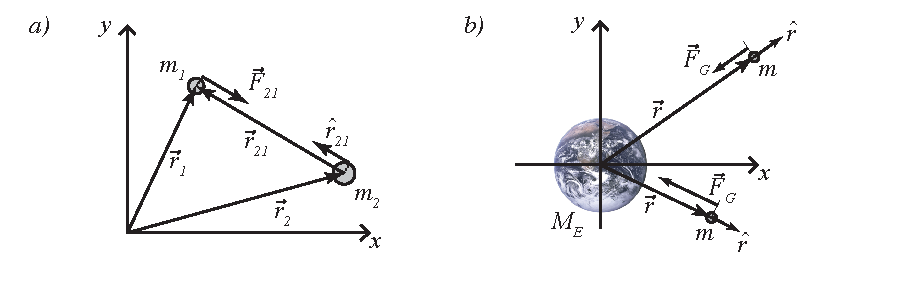
\epsfig{file=NewtonZwaartekracht.pdf, width=\textwidth}
\caption{{\it a) Zwaartekracht uitgeoefend op object~1 door object~2. b) Hetzelfde indien een van de objecten vele malen
zwaarder is dan de andere.}}
\label{fig:NewtonZwaartekracht}
\end{center}
\end{figure} 

In formulevorm ziet Newton's zwaartkrachtwet die wordt uitgeoefend door een willekeurig object met
massa $m_2$ op een ander object met massa $m_1$ er als volgt uit~(zie Fig.~\ref{fig:NewtonZwaartekracht}~a):
\begin{equation}\label{eq:NewtonZwaartekracht}
\vec{F}_{12} = - G\frac{m_1 m_2}{r_{21}^2}\hat{r}_{21}
\end{equation}
De vector $\hat{r}_{21}$ is gedefinieerd als:
\begin{equation}
\hat{r}_{21} \equiv \frac{\vec{r}_{21}}{|\vec{r}_{21}|}= \frac{\vec{r}_1 - \vec{r}_2}{|\vec{r}_1-\vec{r}_2|} 
\end{equation}
Je kan eenvoudig verifieren door de vectoren te tekenen dat $\hat{r}_{21}$ in de richting staat
van object~$1$ gezien vanuit object~$1$: de kracht staat op deze manier in de goede richting omdat
er nog een min-teken staat voor het geheel. Door Newton's wet te gebruiken kan je snel zien dat
 kracht die op object $2$ wordt uitgeoefend door object~$1$ even groot is, maar tegengesteld van 
 teken (\emph{Waarom moet dit wel zo zijn?}). De evenredigheidsconstante $G$ die je ziet voor  
 vgl.~\ref{eq:NewtonZwaartekracht} heet Newton's constante en zijn waarde is:
 \begin{equation}
 G = 6.67\cdot10^{-11}\,N\cdot m^2/kg^2
 \end{equation}
Deze constante zorgt ervoor dat je uiteindelijke kracht de juiste dimensie en grootte in Newtons krijgt. 

In het verder verloop van dit college zullen we meestal 'iets' met zwaartekracht gaan berekenen in het
geval een van de objecten zeer zwaar is, en de andere relatief dus zeer licht. In dat geval kunnen we aannemen
dat het zwaarste van de twee objecten niet significant zal worden beinvloed door het lichtere object. Voor
het gemak, en zonder verlies van precisie kunnen we dan de oorsprong van het coordinatensysteem leggen in het 
centrum van het zware object, en veronderstellen dat dit punt stationair is, zoals getekend in Fig.~\ref{fig:NewtonZwaartekracht}~b).

In het geval van bijvoorbeeld het draaien van een object zoals een satelliet met $m$ om de aarde met $M_E$
is deze benadering uitstekend en reduceert Newtons wet tot:
\begin{equation}\label{eq:NewtonZwaartekracht2}
\vec{F}_{G} = - G\frac{m M_E}{r^2}\hat{r}
\end{equation}
Ook voor bijvoorbeeld de beweging van planeten om de zon is deze benadering prima in de meeste gevallen.
Uiteraard wordt de veronderstelling dat het 'zware' object stilstaat in het centrum van je $CM$ systeem onnauwkeuriger
naarmate de objecten die er omheen draaien zwaarder zijn.

\begin{center}
\line(1,0){250}
\end{center}
\begin{voorbeeld} 
Bepaal met behulp van Newton's wet de massa van de aarde.

{\bf Oplossing: }{\it We weten de valversnelling op het oppervlak van de aarde: $g=9.8m/s^2$. Dus:
\begin{equation}
|\vec{F}_G| = m\,g
\end{equation}
Verder weten we 
de straal van de aarde $r_E=6\cdot 10^6~m$ (Deze kon al tamelijk nauwkeurig worden bepaald door geleerden
in de oudheid. Kan je bedenken hoe ze dat gedaan zouden hebben?). We kunnen vgl.~\ref{eq:NewtonZwaartekracht2} herschrijven tot:
\begin{equation}
M_E = \frac{|\vec{F}_G| r_E^2}{m G}
\end{equation}
Combinatie van de twee vergelijkingen geeft:
\begin{equation}
M_E  =\frac{g \, r_E^2}{G} \approx 5\cdot 10^{24}\,kg
\end{equation}
En dus hebben we de aarde 'gewogen'.
}
\end{voorbeeld}
\begin{center}
\line(1,0){250}
\end{center}

De zwaartekracht zorgt ervoor dat wij naar de aarde worden getrokken, en het is dezelfde kracht die ervoor
zorgt dat planeten om de zon draaien, de maan en satellieten om de aarde, etc etc. We kunnen nu eens kijken 
hoe een object - i.e. satelliet - om de aarde beweegt. Laten we aannemen dat de baan van het object in goede
benadering wordt beschreven met een eenparige cirkelbeweging met straal $r$. We hebben dan volgens 
vgl.~\ref{eq:fc_cirkel} een centripetaalkracht nodig die er uitziet als:
\begin{equation}
\vec{F}_C = -\frac{m\,|\vec{v}|^2}{r}\hat{r}
\end{equation}
Hierin is $|\vec{v}|$ de constante grootte van de baansnelheid.  De enige kracht die de centripetaal versnelling kan
verzorgen is uiteraard de zwaartekracht in dit geval. Dus:
\begin{equation}
-\frac{m\,|\vec{v}|^2}{r}\hat{r} =  - G\frac{m M_E}{r^2}\hat{r}
\end{equation}
Als we de straal van de baan weten kunnen we onmiddellijk de snelheid van de satelliet bepalen:
\begin{equation}
|\vec{v}| = \sqrt{\frac{G M_E}{r}}
\end{equation}
De snelheid hangt niet af van de massa van het object, maar van de massa van de aarde in dit geval, de
zwaartekrachtsconstante, en de straal van de baan. Hoe dichter je bij de aarde komt hoe sneller je 
moet bewegen om in een baan om de aarde te blijven. 

\begin{center}
\line(1,0){250}
\end{center}
\begin{voorbeeld} 
Bereken de straal van de baan van een geostationaire satelliet.

{\bf Oplossing: }{\it We zijn op zoek naar een baan waarvoor geldt dat de omlooptijd net zo lang is als een dag 
op aarde: $T=24~uur$ dus. Als we nu de straal van de baan die we zoeken  $R$ noemen. Dan moet de snelheid gelijk zijn
aan:
\begin{equation}
|\vec{v}| = \frac{2\pi\,R}{T}
\end{equation}
Als we verder aannemen dat de baan cirkelvormig is dan geldt:
\begin{equation}
\frac{|\vec{v}|^2}{R} = \frac{G M_E}{R^2}
\end{equation}
We kunnen nu $|\vec{v}|$ elimineren om te komen tot:
\begin{eqnarray}
\frac{(2\pi\,R)^2}{R\,T^2} & = & \frac{G M_E}{R^2} \\
& \Downarrow & \\
R & = & \left(\frac{G\,M_E\,T^2}{4\pi^2}\right)^{\frac{1}{3}} \approx 4\cdot 10^4~km
\end{eqnarray}

}
\end{voorbeeld}
\begin{center}
\line(1,0){250}
\end{center}

Een belangrijke observatie die je maak als je kijkt naar beelden uit bijvoorbeeld het ISS~\footnote{International
Space Station} is dat alles zich bevindt in een toestand van gewichtsloosheid. Hoe zit dat nou precies? Een
 vaak gehoord argument is dat je gewichtloos bent omdat je ver bent verwijderd van de aarde. Laten we
 eens kijken hoe groot de zwaartekracht ten gevolge van de aarde is als je in het ISS zit. De hoogte waarop
 het ISS rondjes om de aarde draait is ongeveer $h=300~km$ (lage baan dus). Het relatieve verschil van de 
 zwaartekrachtsversnelling op deze hoogte ten opzichte van de versnelling op het aardoppervlak wordt 
 gegeven door:
 \begin{equation}
 \delta \, g \equiv \frac{g(h)-g(h_0)}{g(h_0)} = -\frac{2\,r_E\,h+h^2}{(r_E+h)^2} \approx 5\%
 \end{equation} 
Dat scheelt dus niet zoveel. We moeten ons nu eens afvragen wat gewicht nou precies is. Gewicht is de kracht die
wij uitoefenen op een weegschaal ten gevolge van de zwaartekracht. Als zowel de weegschaal als het object
dat je wil wegen in vrije val zijn, dan drukt het object de weegschaal niet meer in. In vrije val ben je dus
gewichtsloos. Dit is precies hoe een object rond bijvoorbeeld de aarde beweegt: in vrije val. De snelheid van 
het object is in een gesloten baan zodanig dat een object als het ware 'om de aarde' heen valt. Het is dus de hoge
snelheid van een satelliet die ervoor verantwoordelijk is dat deze niet op de aarde stort.

\section{Zwaartekracht potentiele energie}

Laten we nu eens kijken hoe het zit met de arbeid $W$ die je moet verrichten om een object te bewegen
wanneer de zwaartekracht er op werkt. Daarvoor moeten we terugkijken naar de definitie van arbeid zoals
gegeven in vgl.~\ref{eq:defwork}. We zien dat voor de arbeid geldt:
\begin{eqnarray}
W & = & \int_1^2 \vec{F}\cdot d\vec{\ell}\\
    & = &  = - G\,m\,M_E\int_1^2 \frac{\hat{r}\cdot d\vec{\ell}}{r^2}
\end{eqnarray}
 \begin{figure}[htbp]
\begin{center}
  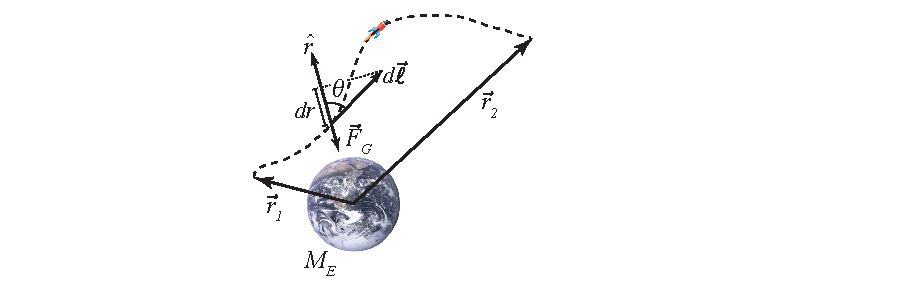
\epsfig{file=NewtonPotentieleEnergie.pdf, width=\textwidth}
\caption{{\it Berekenen van $W$ ten gevolge van zwaartekracht.}}
\label{fig:NewtonPotentieleEnergie}
\end{center}
\end{figure} 
Voor de tweede vergelijking hebben we niets anders gedaan dan het invullen van Newton's zwaartekrachtswet.
De integraal ziet er akelig uit met het inproduct van $\hat{r}$ en $d\vec{\ell}$, dus laten we daar maar eens 
in meer detail naar kijken (zie Fig.~\ref{fig:NewtonPotentieleEnergie}). We kunnen het inproduct schrijven als:
\begin{eqnarray}
\hat{r} \cdot d\vec{\ell} & = & |\hat{r}||d\vec{\ell}|\cos\theta \\ 
& = & |d\vec{\ell}|\cos\theta
\end{eqnarray}
En dit is niets anders dan het stukje van $d\vec{\ell}$ dat in de richting staat van $\hat{r}$, ofwel $dr$. De arbeid
energie schrijven we nu als:
\begin{eqnarray}
W & = & - G\,m\,M_E \int_{|\vec{r}_1|}^{|\vec{r}_2|} \frac{dr}{r^2} \\
     & = & G\,m\,M_E\left(\frac{1}{r_2}-\frac{1}{r_1}\right)
\end{eqnarray}     
De eerste observatie die je hier kan maken is dat de arbeid $W$ alleen maar afhangt van de coordinaten
van het begin en eindpunt van het afgelegde pad. Zwaartekracht is dus een \emph{conservatieve} kracht. Dit
geldt trouwens voor andere soortgelijke centrale krachten, die ook alleen afhangen van $r$, zoals bijvoorbeeld de
elektrische kracht.

Omdat we te maken hebben met een conservatieve kracht, kunnen nu net als in hoofdstuk~\ref{chap:energie} 
een potentiaal identificeren behorend bij de zwaartekracht. Er geldt immers:
\begin{equation}\label{eq:gpot}
\Delta U = -W
\end{equation}
Voor de potentiele zwaartekrachtsenergie kunnen we dus definieren:
\begin{equation}
U(r) = -\frac{G m M_E}{r}
\end{equation}
We zouden een constante waarde kunnen optellen bij onze potentiele energie en nog steeds voldoen
aan vgl.~\ref{eq:gpot}. Deze constante waarde kiezen we 'nul': de moraal is dat alleen verschillen
in potentiele energie relevant zijn, niet de absolute waarde.  We hebben nu onze potentiele energie gedefinieerd
en als een object beweegt onder invloed van de zwaartekracht (geen wrijving en dergelijke) dan
geldt wederom behoud van mechanische energie:
\begin{equation}
K+U=\mbox{Constant}
\end{equation}

\begin{center}
\line(1,0){250}
\end{center}
\begin{voorbeeld} 
Gebruik behoud van energie om de minimale snelheid uit te rekenen zodat een raket afgeschoten vanaf
het aardoppervlak tot $r=\infty$ kan komen.

{\bf Oplossing:}{\it Bij afschieten heeft de raket met snelheid $|\vec{v}_0$ een energie van:
\begin{equation}
E(r=r_E) = K + U = \frac{1}{2}\,m\,|\vec{v}_0|^2-\frac{G\,m\,M_E}{r_E} 
\end{equation}
Met zoals gebruikelijk $M_E$ en $r_E$ de massa en straal van de aarde. Als we willen dat de raket 
naar $r=\infty$ vliegt, dan nemen we maar aan dat $\vec{v}(r=\infty)=\vec{0}$: ofwel de totale energie
is nul als de raket eenmaal oneindig ver weg is gekomen. We moeten dus de snelheid $|\vec{v}_0|$ zodanig
kiezen dat:
\begin{eqnarray}
E(r=r_E) & = & E(r=\infty) = 0 \\
\frac{1}{2}\,m\,|\vec{v}_0|^2-\frac{G\,m\,M_E}{r_E}  & = & 0 \\
& \Downarrow & \\
|\vec{v}_0| & = & \sqrt{\frac{2\,G\,M_E}{r_E}}
\end{eqnarray}
Deze snelheid staat bekend als de ontsnappingssnelheid, en voor de aarde bedraagt deze ongeveer
$11~km/s$ ({\it reken maar na}).
}
\end{voorbeeld}
\begin{center}
\line(1,0){250}
\end{center}

\section{Baanimpulsmoment}

In deze paragraaf wordt iets dieper ingegaan op de beweging van een object ten gevolge van een centrale
kracht (in dit geval zwaartekracht). Deze analyse zal aantonen dat er naast impuls en energie nog een $3^e$
behouden grootheid in het spel is: namelijk het impulsmoment van een object. De afleiding is tamelijk
formeel, dus zet je maar schrap.

We beginnen met het opschrijven van Newtons $2^e$ wet in poolcoordinaten:
\begin{eqnarray}
\vec{F} & = & m\vec{a} \\
\vec{F}_r + \vec{F}_{\phi} & = & m\left(\vec{a}_{r} + \vec{a}_{\phi}\right)
\end{eqnarray}
We hebben nog niets gedaan, behalve het ontbinden van zowel kracht als versnelling in een radiele ($r$)
en een tangentiele ($\phi$) component.  Maar we zien onmiddellijk dat in het geval van een centrale 
kracht, dat $\vec{F}_{\phi}=\vec{0}$: een centrale kracht heeft slechts een radiele component. Nu zie je
waarom het gerbuik van poolcoordinaten in dit geval superieur is boven het gebruik van ordinaire cartesische
coordinaten.  Er valt zomaar een term weg uit je vergelijkingen, terwijl dit in cartesische coordinaten niet
zou gebeuren. Let wel op: je kan natuurlijk het probleem prima beschrijven in cartesische coordinaten en
je zal ook wel dezelfde antwoorden vinden, maar de vergelijkingen die je krijgt  zijn minder 'transparant'. 
Nu kunnen we eens kijken naar de rechterkant van de vergelijking. Met behulp van vgl.~\ref{eq:apool}
krijgen we de volgende twee vergelijkingen:
\begin{equation}
\left\{\begin{array}{ccc}
\vec{F}_r & = & m\left(\frac{d^2r}{dt^2} - r\left(\frac{d\phi}{dt}\right)^2\right)\hat{r} \\
\vec{0} & = & m\left(2 \frac{dr}{dt}\frac{d\phi}{dt}+r\frac{d^2\phi}{dt^2}\right)\hat{\phi}
\end{array}\right.
\end{equation}
Je ziet dat de tweede vergelijking laat zien dat de tangentiele versnelling nul moet zijn. Dit betekent niet dat
de hoek $\phi$ niet verandert. Sterker nog, dit betekent zelfs niet dat $d^2\phi / dt^2=0$(!), zoals je kan zien
aan de vergelijking. Het is nu mogelijk om de vergelijking voor de $\hat{\phi}$ versnelling op vernuftige wijze
te herschrijven als een totale tijdsafgeleide ({\it verifieer deze vergelijking}):
\begin{equation}\label{eq:dLdt}
0 = m\frac{d}{dt}\left(r^2\frac{d\phi}{dt}\right) \hat{\phi} \equiv \frac{dL}{dt} \hat{\phi}
\end{equation}
Het product $m r^2 d\phi/dt$ staat bekend als het baanimpulsmoment van een object, en deze grootheid
hebben we al eerder gezien:
\begin{equation}
L \equiv m r^2 \frac{d\phi}{dt}
\end{equation}
We hebben al eerder gezien dat het impulsmoment een vector is, maar op dit moment is het voldoende om alleen naar de grootte van
deze vector te kijken. Je ziet namelijk in vgl.~\ref{eq:dLdt} dat de afgeleide naar de tijd van het 
impulsmoment nul is. En als de afgeleide nul is moet dus gelden voor een centrale kracht:
\begin{equation}
L = \mbox{constant}
\end{equation}
Als je het impulsmoment op een moment kent, dan ken je deze voor een willekeurig ander moment.
$L$ is namelijk hetzelfde. Voor een eenparige cirkelbeweging is dit evident: de straal van de baan is constant,
net als de hoeksnelheid $d\phi/dt$: $L$ is dus constant. Maar omdat we in onze afleiding geen
enkele aanname hebben gemaakt over de exacte vorm van de baan, geldt behoud van impulsmoment
veel algemener. De meeste planeten in ons zonnestelsel beschrijven geen perfecte cirkelbanen, maar 
ze bewegen over elliptische paden. $L$ is behouden, en je weet dan dat als bijvoorbeeld $r$ voor een
deel van de baan kleiner is, dat op dat moment $d\phi / dt$ dus groter moet zijn. Je kan dit trouwens ook
wel een aanvoelen, omdat een planeet dichter bij de zon minder potentiele energie heeft dan op een
grotere afstand. We weten dat energie is behouden en dus kan het niet anders zijn dan dat de snelheid
voor de kleinere afstand groter is geworden.

\begin{center}
\line(1,0){250}
\end{center}
\begin{voorbeeld} 
Een balletje met massa $m$ is bevestigd aan een touw en draait zonder wrijving rondjes met constante snelheid $\vec{v}_0$
op afstand $r_0$ zoals in Fig.~\ref{fig:ImpulsMoment}. Door aan het touw te trekken wordt de afstand $r_1$. Wat is nu de
snelheid $|\vec{v}_1|$?
 \begin{figure}[htbp]
\begin{center}
  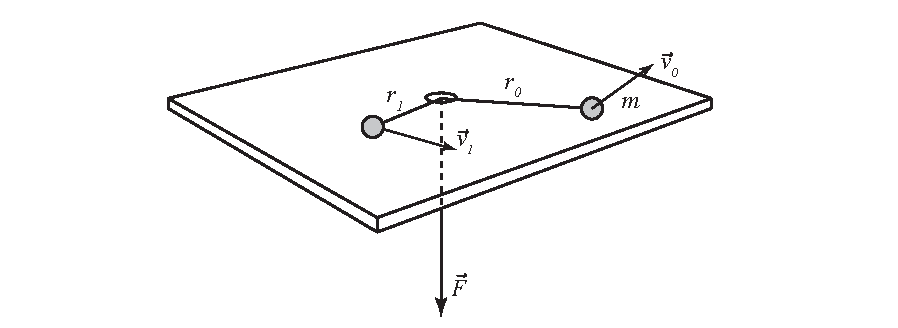
\epsfig{file=ImpulsMoment.pdf, width=\textwidth}
\caption{{\it Behoud van impulsmoment voor een balletje aan een touw.}}
\label{fig:ImpulsMoment}
\end{center}
\end{figure} 

{\bf Oplossing: }{\it  Het balletje wordt in de bocht gehouden door de centripetaalkracht die wordt geleverd door aan het 
touw te trekken met kracht $\vec{F}$. De centripetaalkracht is alleen radieel gericht en dus is impulsmoment behouden.
Op $t=0$ geldt:
\begin{equation}
L = m r_0^2 \frac{d\phi}{dt} = m r_0^2 \frac{|\vec{v}_0|}{r_0} = m r_0 |\vec{v}_0|
\end{equation}
Waarbij we gebruiken dat $\vec{v}_ = (d\phi / dt) r_0 \hat{\phi}$. Nadat de straal is veranderd naar $r_1$ geldt:
\begin{equation}
L = m r_1 |\vec{v}_1|
\end{equation}
En dus:
\begin{equation}
|\vec{v}_1| = |\vec{v}_0| \frac{r_0}{r_1}
\end{equation}
}
\end{voorbeeld}
\begin{center}
\line(1,0){250}
\end{center}

\section{Banen van de planeten}

Dit hoofdstuk wordt afgesloten met een korte beschouwing van de beweging van objecten bij een centrale kracht,
zoals bijvoorbeeld geldt voor de beweging van een planeet m de zon. We kijken hiervoor naar de totale energie
van een object $E$, die zoals wij weten behouden is int dit geval. Dus:
\begin{equation}\label{eq:etot_grav}
E = \frac{1}{2}m|\vec{v}|^2 + U(r)
\end{equation}
De kinetische energie $K$ wordt geschreven als (\emph{volg afleiding maar eens stap voor stap}) :
\begin{eqnarray}
\frac{1}{2} m|\vec{v}|^2 & = & \frac{1}{2}m (\vec{v}_{r}+\vec{v}_{\phi})\cdot(\vec{v}_{r}+\vec{v}_{\phi}) \\
& = & \frac{1}{2}m (\vec{v}_r\cdot\vec{v}_r + 2 \vec{v}_r\cdot\vec{v}_{\phi} + \vec{v}_{\phi}\cdot\vec{v}_{\phi}) \\ 
& = & \frac{1}{2}m (|\vec{v}_r|^2 + |\vec{v}_{\phi}|^2) \\
& = & \frac{1}{2}m\left\{\left(\frac{dr}{dt}\right)^2+r^2\left(\frac{d\phi}{dt}\right)^2\right\} \\
& = & \frac{1}{2}m\left\{\left(\frac{dr}{dt}\right)^2+\frac{L^2}{(m\,r)^2}\right\}
\end{eqnarray}
We hebben dus de kinetische energie herschreven in een term met de radiele snelheid en het impulsmoment. Dit
gaat ons enorm helpen in verdere berekeningen omdat $L$ niet verandert. Als we deze uitdrukking voor de
kinetische energie invullen in vgl.~\ref{eq:etot_grav} krijgen we:
\begin{equation}
E = \frac{1}{2} m\left(\frac{dr}{dt}\right)^2+\frac{L^2}{2\,m\,r^2} + U(r) \equiv \frac{1}{2} m\left(\frac{dr}{dt}\right)^2 + U_{eff}(r)
\end{equation}
Hoewel je dat misschien niet meteen ziet, kan deze uitdrukking worden gebruikt om op te lossen langs wat voor 
pad een object in een centrale potentiaal beweegt. We kunnen namelijk een uitdrukking vinden voor $dr/dt$:
\begin{equation}
\frac{dr}{dt} = \sqrt{\frac{2}{m}\left(E-U_{eff}(r)\right)}
\end{equation}
Verder kunnen we de definitie van $L$ gebruiken om ook voor $d\phi / dt$ een mooie uitdrukking te vinden:
\begin{eqnarray}
L & = & m r^2 \left(\frac{d\phi}{dt}\right)^2 \\
& \Downarrow & \\
\frac{d\phi}{dt} & = & \frac{L}{m\,r^2}
\end{eqnarray}
Door combinatie van de twee laatste vergelijkingen krijgen we een uitdrukking die de baan van bijvoorbeeld
een planeet  beschrijft:
\begin{equation}
\frac{d r}{d\phi} = \frac{\sqrt{(2/m)(E-U_{eff}(r))}}{L/mr^2}
\end{equation}
Deze vergelijking hangt alleen maar af van $r$, terwijl de waarden van de totale energie en het impulsmoment
voor een bepaalde baan van een object moeten worden vastgelegd, of gekozen (ze veranderen niet). Het blijkt
dat de krommen die $r$ beschrijven als functie van $\phi$ ofwel cirkelbanen, ofwel ellipsen ofwel hyperbolen 
zijn~\footnote{Afleiding hiervan bevat geen nieuwe fysische concepten, maar is geometrisch lastig. Slaan we voor dit
college over.} 
De baan van de maan om de aarde, en van de planeten om de zon, maar ook het vallen van objecten op
aarde kunnen op deze manier door Newton's wet van universele zwaartekracht worden beschreven. Deze beschrijving
van meerdere fysische observaties vanuit een universeel principe is een fenomenale doorbraak in de natuurkunde 
geweest.

\section{Wat moet ik weten en kunnen?}

Na dit hoofdstuk moet je weten:
\begin{itemize}
\item Hoe een centrale kracht eruit ziet, en in het bijzonder de Newton's zwaartekrachtswet.
\item Hoe de potentiele energie eruit ziet voor een centrale kracht. 
\item Wat impulsmoment is.
\item Waarom Newton een 'grote jongen' is.
\end{itemize}
Je moet kunnen:
\begin{itemize}
\item Rekenen met centrale krachten en bijbehorende potentiele energie.
\item Rekenen met impulsmoment.
\end{itemize}

\section{Opgaven}

\begin{enumerate}
\item Doorlezen Giancoli paragraaf 6-5.
\item Giancoli Hoofdstuk 6: 11, 16, 17, 18, 34, 63, 66, 69, 70, 74, 
\item Giancoli Hoofdstuk 8: 45, 47, 48, 52, 58, 60, 99, 100,  
\item Bepaal het gewicht van iemand met massa $m$ die (i) op de noordpool van de aarde staat en die (ii) op
de evenaar van de aarde staat.
\end{enumerate}

%%%%%%%%%%%%%%%%%%%%%%%%%%%%%%%%%%%%%%%%%%%%%%%
% EINDE GRAVITATIE
%%%%%%%%%%%%%%%%%%%%%%%%%%%%%%%%%%%%%%%%%%%%%%%

%%%%%%%%%%%%%%%%%%%%%%%%%%%%%%%%%%%%%%%%%%%%%%%
% BEGIN STATISCH EVENWICHT
%%%%%%%%%%%%%%%%%%%%%%%%%%%%%%%%%%%%%%%%%%%%%%%
\chapter{Statisch evenwicht}

Dit college wordt afgesloten met een korte verhandeling over statisch evenwicht. Je zal leren
wat de voorwaarden zijn voor evenwicht en hoe daar mee valt te rekenen. Het hoofdstuk gaat
in zekere zin verder waar hoofdstuk~\ref{chap:newton} is gestopt. Je moet weer gedetailleerde
krachten analyses maken om problemen te doorgronden.
Stof uit Giancoli:
\begin{itemize}
\item Hoofdstuk 12.1 - 12.2
\end{itemize}

\section{Krachtmoment}

In deze paragraaf geven we een simpele definitie van het begrip krachtmoment, dat je
wellicht eerder hebt gezien tijdens VWO natuurkunde. 
 \begin{figure}[htbp]
\begin{center}
  
\epsfig{file=Krachtmoment.pdf, width=\textwidth}
\caption{{\it Variabelen benodigd voor de definitie van het krachtmoment.}}
\label{fig:torque}
\end{center}
\end{figure} 
Als je een object hebt zoals
bijvoorbeeld getekend in Fig.~\ref{fig:torque} waarop een kracht aangrijpt niet in het
zwaartepunt dan is het krachtmoment, $|\vec{\tau}|$ gedefinieerd als de 'kracht maal de 
arm', $d$, waarover deze kracht wordt uitgeoefend. Ofwel:
\begin{equation}
|\vec{\tau}| = |\vec{F}|\,d =|\vec{F}||\vec{r}|\sin\theta
\end{equation}
Let op dat hier expliciet over de grootte van het krachtmoment wordt gesproken. Wat in dit
college achterwege wordt gelaten is het vector-karakter van het krachtmoment. Al er een 
netto krachtmoment op een object wordt uitgeoefend kan een object gaan draaien om een 
bepaalde as. De dynamica van de draaibeweging echter, zoals die in hoofdstuk~11 van Giancoli
wordt besproken wordt voor dit college overgeslagen, maar komt in het $2^e$ jaar aan bod
tijdens het voortgezette klassieke mechanica college.  We gaan draaimomenten alleen
maar gebruiken voor onze studie van statisch evenwicht.                  

\section{Voorwaarden voor evenwicht}

Een goede vraag om mee te beginnen is, wat nou precies een statisch evenwicht is. In het 
kader van dit college verstaan we onder een  statische evenwicht een situatie waarbij een 
object in stilstand is, en dat ook blijft. Op zich klinkt een dergelijke situatie tranentrekkend saai, 
maar wat je in het algemeen leert van het onderzoeken van een evenwicht is wat voor krachten
er in en op een object worden uitgeoefend. Deze kennis is van levensbelang voor ingenieurs
die een brug of gebouw ontwerpen.

De eerste conditie waaraan een object moet voldoen, wil het in evenwicht zijn, is dat de som 
van alle krachten op dat object gelijk moet zijn aan nul:
\begin{equation}
\sum_i \vec{F}_i = \vec{0}
\end{equation}
Als dit niet het geval is dan gaat een object versnellen en is het dus niet in evenwicht.

Nu zou je misschien zeggen dat een object waarop de eerste conditie van toepassing is niet
gaat bewegen, maar dit is niet altijd het geval. De eerste conditie geeft enkel aan dat het 
zwaartepunt van een object niet van z'n plek komt, maar een object kan nog steeds gaan
draaien, als er een netto krachtmoment $\tau$ op het object werkt. Dus de tweede conditie
voor een statisch evenwicht is niet verrassend:
\begin{equation}
\sum_i \tau_i = 0
\end{equation}
De som van alle krachtmomenten om een bepaalde draaias moet gelijk nul zijn. Dit is alle
theorie die je nodig hebt voor het bestuderen van statische evenwichten. In het algemeen 
leveren beide evenwichtsvoorwaarden je een set van vergelijkingen op, waarmee je alle
krachten in een systeem kan bepalen. In de volgende paragraaf volgen een paar voorbeelden.

\section{Selectie van voorbeelden}

De voorbeelden 12-3, 12-5 en 12-6 uit Giancoli worden tijdens het college behandeld. 

\section{Wat moet ik weten en kunnen}

Je moet weten:
\begin{itemize}
\item Wat is krachtmoment.
\item Wat zijn de twee voorwaarden voor een statisch evenwicht.
\end{itemize}
Je moet kunnen:
\begin{itemize}
\item Analyseren hoe een evenwicht werkt.
\item Uitrekenen hoe groot de krachten zijn in eenvoudige problemen.
\end{itemize}

\section{Opgaven}

\begin{enumerate}
\item Giancoli hoofdstuk~12: 1, 11, 18, 22, 27, 32, 59, 62, 68, 70, 84, 85, 93, 95.
\end{enumerate}

%%%%%%%%%%%%%%%%%%%%%%%%%%%%%%%%%%%%%%%%%%%%%%%
% EINDE STATISCH EVENWICHT
%%%%%%%%%%%%%%%%%%%%%%%%%%%%%%%%%%%%%%%%%%%%%%%


\part{Speciale Relativiteits Theorie}

\chapter*{Inleiding}
\addcontentsline{toc}{chapter}{Inleiding}

\section*{Waar hebben we het over?}

Het college klassieke mechanica en speciale relativiteitstheorie behandelt in parallel twee belangrijke 
onderwerpen uit de natuurkunde. Aan de ene kant komt de klassieke natuurkunde aan bod, waarin de
basis wordt gelegd voor in principe \emph{alle} vervolgvakken in het curriculum. Er wordt bekeken hoe
het 'bewegen' van objecten nou precies werkt. Hiervoor gaan we de drie wetten van Newton bestuderen
die het hart vormen van de klassieke mechanica. Belangrijke begrippen als eenparige beweging, 
eenparig versnelde beweging, energie en impuls worden behandeld. Deze begrippen zijn zo algemeen
dat ze ook buiten de klassieke mechanica van essentieel belang zijn. Het heeft eigenlijk geen zin om 
geavanceerde vakken als quantummechanica te bestuderen zonder een degelijk begrip van de klassieke
mechanica. 

De andere helft van dit vak behandelt de speciale relativiteitstheorie van Einstein. In dit vak gaan we over
de grenzen van de klassieke mechanica en maken we een paar gewaagde aannames. Redenaties op 
basis van deze aannames leidt tot conclusies over ruimte en tijd die in perfecte tegenspraak zijn met
ons gevoel hoe de natuur 'zou moeten werken'. We gaan onderzoeken of de debiele conclusies die
we moeten trekken zijn gerechtvaardigd en ook zullen we de samenhang tussen de relativiteitstheorie en
de klassieke mechanica onderzoeken.

\section*{Wat wordt er van jullie verwacht?}

In het algemeen zijn de vakken die worden onderwezen tijdens het 1e jaar van de bachelor zogenaamde 
stapelvakken: zonder kennis van het ene  vak is het moeilijk een begin te maken met het volgende. En zelfs
binnen een vak is het vaak zo dat het missen van \'{e}\'{e}n college het volgen van de rest verhindert. Er 
wordt daarom van jullie verwacht dat je actief meedoet aan liefst alle colleges en werkcolleges. In de
college's wordt de stof behandeld die je moet weten, en worden er enkele voorbeelden uitgewerkt. Tijdens
een werkcollege moet je zelf aan de slag. Met name het maken van opgaven is erg lastig in het begin, omdat
je soms niet echt een gevoel hebt hoe en waar je aan natuurkundige problemen moet beginnen.  Enig 
doorzettingsvermogen is handig op dit punt. 

Naast de contacturen wordt er van jullie verwacht dat je werkt aan het college. De richtlijn is dat je aan 'zelfstudie'
ongeveer evenveel tijd besteedt als aan colleges+werkcolleges. Dit klinkt als veel tijd en dat is het ook. Het
blijkt soms moeilijk om je hiervoor te motiveren, maar de docenten gaan er wel vanuit dat deze tijd ook echt
in de colleges wordt geinvesteerd door jullie.

\section*{Wat is lastig?}

Er zijn een paar valkuilen waar je in kan trappen tijdens dit college en waardoor je het jezelf extra lastig kan 
maken. Sommige van deze valkuilen horen specifiek bit dit vak, en  andere valkuilen zijn meer algemeen
geldig voor de studie natuurkunde. Bij deze een selectie gemaakt door jullie docenten:
\begin{itemize}
\item{\bf Klassieke mechanica ken ik al van het VWO.}  Vaak gehoorde klacht is dat je alles al zou kennen. Het
is natuurlijk deels waar dat je een deel van de klassieke mechanica al eens eerder gezien hebt op het VWO, maar
tijdens de natuurkunde studie zal je voor het eerste de interne samenhang van de theorie onderzoeken. Bovendien
is het niveau van het college veel abstracter en gaan we dieper op de stof in.
\item{\bf Tijd en zelfstudie.}  Het blijkt lastig om zelf aan vakken te werken buiten de colleges om. Moet toch, maar
vraagt discipline.
\item{\bf Het rekenbeest.} Bijna niet nodig.
\item{\bf Formules en getallen.} Gerelateerd aan het vorige punt. We rekenen vaak formules uit, en we vragen
lang niet altijd om een numeriek resultaat. Het grote voordeel van het werken en rekenen met formules is dat je
antwoorden krijgt die algemeen geldig zijn ipv voor een enkel voorbeeld.  
\end{itemize}

\section*{Opzet van het college}

Zoals hierboven al genoemd volgt dit college de klassieke opzet van een hoorcollege in combinatie met 
werkcolleges.  Per week worden er $2\times2$ uur college gegeven, met een werkcollege bij ieder
hoorcollege. De werkcolleges gebeuren in een kleinere setting, waarbij je in een groep van ongeveer
25 studenten wordt geholpen door je "eigen" assistent. De toetsing van het college gebeurt door
middel van een tentamen aan het eind.  Daarnaast is er halverwege de cursus een deeltentamen en wordt
er van jullie verwacht dat er iedere week digitale opgaven worden gemaakt.




\chapter{De Galileitransformatie}
\vspace{-1cm}\begin{flushright}
{\it `Philosophy is written in this grand book \\-I mean the
  Universe-\\it is written in the language of mathematics.'}\\
 G. Galilei\end{flushright}
Gebeurtenissen spelen zich af op zekere plaatsen en tijdstippen.
Een plaats beschrijven we t.o.v. een co\"{o}rdinatenstelsel en tijd meten we 
met een klok.

% \begin{figure}[h]
% \begin{center}
% \mbox{\epsfxsize=10cm\epsffile{syllabus.pictures/xyzr.eps}}
% \caption{Driedimensionaal, orthogonaal co\"{o}rdinatenstelsel}
% \label{f:galilei1}
% \end{center}
% \end{figure}

\section{Co\"ordinatenstelsel}
Het is duidelijk dat de keuze van een specifiek co\"ordinatenstelsel,
ten opzichte waarvan beweging wordt beschreven, geheel vrij is. Het
verdient natuurlijk de voorkeur een co\"ordinatenstelsel te kiezen
waarin de beschrijving van beweging het gemakkelijkst is. De
bewegingen van de conducteur op een trein bijvoorbeeld, worden het
makkelijkst beschreven in een stelsel waarin de trein zelf
stilstaat. De eenparige beweging van de trein ten opzichte van
een co\"ordinatenstelsel verbonden met de aarde wordt (in het ideale
geval) tenslotte niet eens opgemerkt.


\begin{figure}[ht]
\centering
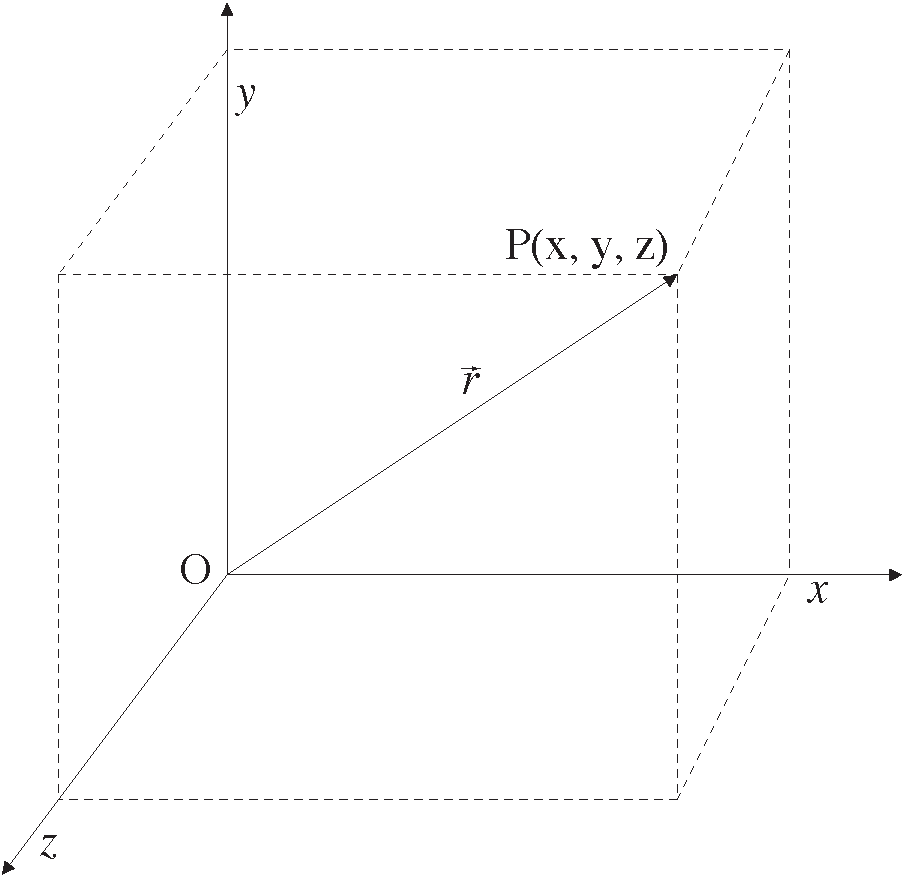
\epsfig{file=xyzr.pdf, width=0.5\textwidth}
\caption{{\sl Driedimensionaal, orthogonaal co\"{o}rdinatenstelsel}}
\label{f:galilei1}
\end{figure}


In figuur~\ref{f:galilei1} is een rechtshandig, orthogonaal,
driedimensionaal co\"{o}rdina-tenstelsel weergegeven.  Een vector
$\vec{r}$ wijst vanuit de oorsprong ${\cal O}$ naar een punt waarvan
de positie door drie getallen, de co\"{o}rdinaten, $x, y$ en $z$ wordt
aangegeven.  (Cartesiaanse co\"ordinaten). Orthogonaal wil zeggen dat de
drie assen loodrecht op elkaar staan.  Rechtshandig wil zeggen dat als
we langs de positieve $z$-as kijken, we de positieve $x$-as naar de
positieve $y$-as roteren met een rechtshandige draai\footnote{Of
bekijk het assenstelsel met uw handen: de positieve $x$-as uw duim, de
$y$-as de wijsvinger en de $z$-as de middelvinger.}.

Natuurlijk kunnen ook andere definities voor de co\"ordinaten gekozen
worden, bijvoorbeeld twee hoeken $\theta$ en $\phi$ ten opzichte van de assen en de
lengte van de vector, $r$ (bolco\"ordinaten). Meer specifiek: de 
poolhoek $\theta$ correspondeert met de hoek tussen de vector en de
$z$-as, de azimuth hoek $\phi$ is de openingshoek met de $x$-as, na projectie van de vector in het $x-y$ vlak.
Deze bolco\"ordinaten kunnen in  Cartesiaanse co\"ordinaten worden getransformeerd via
\begin{eqnarray}
x & = & r \sin \theta \cos \phi \\
y & = & r \sin \theta \sin \phi \\
z & = & r \cos \theta
\end{eqnarray}

Ongeacht de definitie van de co\"ordinaten, zullen er altijd {\em
drie} nodig zijn om een punt te bepalen in de ruimte. Dit is de
essentie van een drie-dimensionale ruimte. We zullen in dit college
verder alleen Cartesiaanse co\"ordinatenstelsels beschouwen. Als notatie 
van een drie-dimensionale vector, $\vec{x}$, gebruiken we een pijltje boven de symboolnaam. De componenten van 
een vector $\vec{x}$ geven we aan met de labels $(x,y,z)$.

Beschouw nu twee Cartesische co\"ordinaatsystemen, met label $S$ en
$S'$, die verschoven en geroteerd zijn ten opzichte van elkaar. Bekijk het geval dat ze 
beide hetzelfde punt in de ruimte beschrijven. In het ene stelsel,
$S$, heeft het punt $\vec{p}$ de co\"ordinaten $(p_x,p_y,p_z)$. Hetzelfde punt beschreven door het andere stelsel $S'$, heet nu $\vec{p}'$ en heeft de co\"ordinaten $(p'_x, p'_y,
p'_z)$. Met andere woorden, de waarden van de co\"ordinaten hangen
af van de keuze van het co\"ordinaatenstelsel. Dit geldt niet voor de
{\sl afstand} tussen twee punten in de ruimte. Deze afstand is
onafhankelijk van de keuze van de oorsprong en rotatie van het co\"ordinaatenstelsel, en wordt
daarom een {\sl invariante} grootheid genoemd. De afstand $\Delta r$ tussen twee
punten $\vec{x}_1$ en $\vec{x}_2$ in Cartesiaanse co\"ordinaten kan
verkregen worden met
\[
\Delta r = \sqrt{ (x_2-x_1)^2+(y_2-y_1)^2+(z_2-z_1)^2 }.
\]
oftewel
\[
(\Delta r)^2 = (\Delta x)^2 + (\Delta y)^2 + (\Delta z)^2
\]
De waarde van deze afstand $\Delta r$ hangt natuurlijk wel van de keuze van
de eenheden af.


% \begin{figure}[h]
% \begin{center}
% \mbox{\epsfxsize=8cm\epsffile{syllabus.pictures/systems.eps}}
% \caption{Tweedimensionaal, orthogonaal co\"{o}rdinatenstelsel $S'$ beweegt
% met constante snelheid $v$ t.o.v. co\"{o}rdinatenstelsel $S$}
% \label{f:galilei2}
% \end{center}
% \end{figure}

\begin{figure}[ht]
\centering
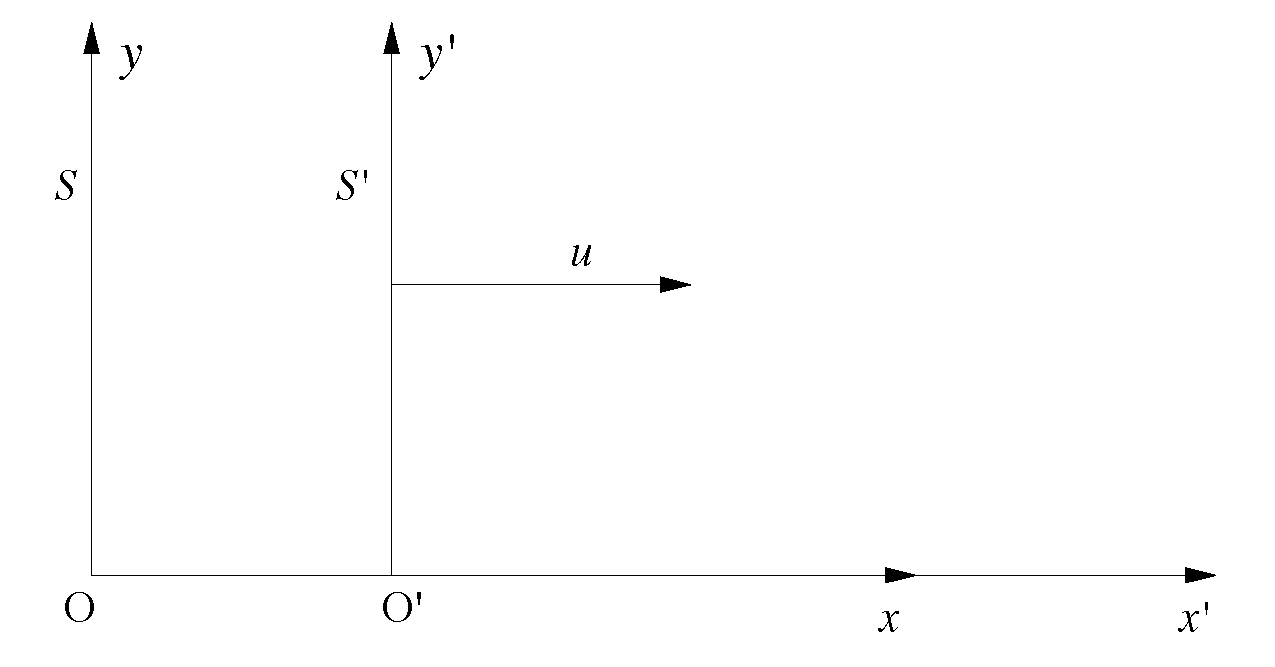
\epsfig{file=systems.pdf, width=0.7\textwidth}
\caption{{\sl Tweedimensionaal, orthogonaal co\"{o}rdinatenstelsel $S'$ beweegt
met constante snelheid $v$ t.o.v. co\"{o}rdinatenstelsel $S$}}
\label{f:galilei2}
\end{figure}

Indien we verschijnselen beschrijven die zich in een plat vlak afspelen 
is een tweedimensionaal co\"{o}rdinatenstelsel voldoende, en een punt
in het platte vlak wordt met twee co\"ordinaten beschreven.
In figuur~\ref{f:galilei2} is een tweedimensionaal co\"{o}rdinatenstelsel $S$ 
getekend en een tweedimensionaal co\"{o}rdinaten-stelsel $S^{'}$ dat met 
constante snelheid $v$ beweegt t.o.v. $S$, in de $x$-richting. Denk
bijvoorbeeld aan een trein bij het station, waarbij stelsel $S$ met
het perron correspondeert, en stelsel $S'$ met de rijdende trein.

We vragen ons nu af hoe we co\"{o}rdinaten (van bijvoorbeeld de baan van 
een puntmassa) gemeten t.o.v. $S$ kunnen uitdrukken in de co\"{o}rdinaten 
(van het zelfde verschijnsel) gemeten t.o.v. $S^{'}$.
Het antwoord kan gemakkelijk worden verkregen:
\begin{eqnarray}
\label{v:galilei1a}
y' &=& y\\
\label{v:galilei1b}
x' &= & x - vt
\end{eqnarray}
waar $t$ de tijd voorstelt (als beginvoorwaarde hebben we gekozen dat op tijd $t=0$ de co\"{o}rdinatenstelsels $S$ en $S^{'}$ samenvallen).

De {\sl snelheid} in de $x$-richting is per definitie de afgeleide 
van de $x$-co\"{o}rdinaat naar de tijd:
\begin{eqnarray*}
V_{x} & \equiv & \frac{dx(t)}{dt}
\end{eqnarray*}
Ten opzichte van $S^{'}$ geldt:
\begin{eqnarray*}
V_{x}^{'} & = &  \frac{dx^{'}}{dt}
\end{eqnarray*}
en dus volgt
\begin{equation}
\label{v:galilei2}
V_{x}^{'} = V_{x} -v
\end{equation}
We hebben als vanzelfsprekend aangenomen dat
\begin{eqnarray*}
t^{'} & = &  t
\end{eqnarray*}
d.w.z. we hebben aangenomen dat de tijd in $S^{'}$ en $S$ op identieke wijze 
verloopt.
Het zal in de loop van dit college blijken dat we deze `vanzelfsprekendheid'
moeten herzien!

Formules~\ref{v:galilei1a} en \ref{v:galilei1b} zijn overigens ook
volstrekt voor de hand liggend (en zoals we in de inleiding al zagen, moeten
herzien): als een fietser zich met snelheid $V_{x}$ over een weg
beweegt (stelsel $S$) en een voetganger (stelsel $S{'}$) zich met een
snelheid $v$ in dezelfde richting over die weg beweegt, dan beweegt de
fietser t.o.v. de voetganger met snelheid $V_{x}^{'} = V_{x} -
v$. Gaan fietser en voetganger even hard, d.w.z. $V_{x} = v$, dan is
hun relatieve snelheid $V_{x}^{'} = 0$. D\'{i}t resultaat zullen we
niet hoeven te herzien!

De {\sl versnelling} is per definitie de afgeleide van de snelheid 
naar de tijd :
\begin{eqnarray*}
a_{x} & \equiv & \frac{dV_{x}}{dt}
\end{eqnarray*}
Omdat $v$ constant is is nu gemakkelijk na te gaan dat:
\begin{equation}
\label{v:galilei3}
a_{x}^{'}  = a_{x}
\end{equation}
Versnellingen, en dus krachten ($\vec{F} = m\vec{a}$), zijn dus gelijk
in $S$ en $S^{'}$.  Meer in het algemeen blijkt dat de wetten van de
mechanica er hetzelfde uitzien in $S$ en $S^{'}$.  Als we hier even
over nadenken is dit een heel bevredigend en gewenst resultaat.  Het
zou een onaantrekkelijk idee zijn dat de natuurwetten zouden afhangen
van de `toevallige' bewegingstoestand van de natuurkundige die deze
wetten opspoort.

Formules~\ref{v:galilei1a} en~\ref{v:galilei1b} staan bekend als de
\textit{Galileitransformatie}.  Met behulp van deze formules kunnen we dus
co\"{o}rdinaten gemeten in het ene co\"{o}rdinatenstelsel,
{\sl transformeren} naar co\"{o}rdinaten in het andere
co\"{o}rdinaten-stelsel.  Wiskundig gezien is deze transformatie heel
eenvoudig, maar natuurkundig gezien is de observatie dat de wetten van
de mechanica hun vorm behouden (`gelijk blijven') van diepgaande
betekenis.  We zouden het als volgt kunnen formuleren: natuurkundig
gezien zijn alle co\"{o}rdinatenstelsels\footnote{We beperken ons in
dit college tot co\"{o}rdinatenstelsels die met constante snelheid (eenparig) ten
opzichte van elkaar bewegen. Co\"ordinaatstelsels die ook
versnellingen t.o.v. elkaar ondergaan worden behandeld in Einsteins
`Algemene Relativiteitstheorie'.} equivalent.  Of nog anders: er is geen
co\"{o}rdinatenstelsel dat onze voorkeur verdient.  

In het voorbeeld van het perron en de rijdende trein betekent dit het
volgende. Indien twee waarnemers ten opzichte van elkaar
eenparig rechtlijnig bewegen (een waarnemer op perron, de ander in de
trein), zullen ze precies dezelfde fysische verschijnselen
meten. Voorwerpen kunnen worden gedraaid en verschoven; hun meetkundige
eigenschappen zijn gelijk. En een voorwerp dat aan zichzelf wordt
overgelaten, d.w.z. waarop geen krachten werken, blijft in rust of beweegt
zich eenparig rechtlijnig. Dit is de definitie van een {\em
  inertiaalsysteem}. De twee waarnemers bevinden zich dus in twee
verschillende inertiaalsystemen. De vraag is nu: verdient een van deze
inertiaalsystemen de voorkeur voor het beschrijven van fysische
processen? Kunnen we de natuurwetten beter beschrijven t.o.v. de
bewegende trein of ten opzichte van het perron? 
De situatie verandert natuurlijk drastisch zodra de trein remt of door
de bocht gaat. Dan beginnen losliggende voorwerpen als `vanzelf' te
bewegen, en is het co\"ordinatenstelsel van de trein geen
inertiaalsysteem meer.

\begin{quote}
Een Cartesiaans ruimtelijk co\"ordinatenstelsel waarin een aan
zichzelf overgelaten voorwerp in rust blijft of eenparig rechtlijnig
beweegt noemen we een {\it inertiaalsysteem}.
\end{quote}
Met behulp van het begrip inertiaalsysteem kunnen we nu het al genoemde relativiteitsprincipe preciezer formuleren:
\begin{quote}
De natuurwetten hebben in elk inertiaalsysteem dezelfde vorm; ze zijn hetzelfde.
\end{quote}
Dit betekent dat alle inertiaalsystemen onderling equivalent zijn. Het betekent ook dat beweging relatief is in de zin dat er geen absoluut onderscheid gemaakt kan worden tussen rust en eenparig rechtlijnige beweging.


Laten we eens kijken of er niet toch inertiaalsystemen zijn die onze
voorkeur hebben voor het beschrijven van de natuurwetten.

\section{Voorkeursstelsel}
Is er een inertiaalsysteem dat onze voorkeur verdient?

Golven, zoals geluidsgolven, bestaan dankzij een {\sl medium}.
Geluidsgolven zijn niets anders dan een periodieke opeenvolging van
verdikkingen en verdunningen van het medium lucht.  Voor
golfverschijnselen blijken er wel degelijk een co\"{o}rdinatenstelsel
te bestaan dat onze voorkeur verdient: het inertiaalsysteem ten
opzichte waarvan het medium in rust is.  Niet alleen is de
vergelijking die de plaats- en tijdsafhankelijkheid van de geluidsgolf
(dus in feite van de luchtdruk) beschrijft (de wiskundige formulering
slaan we over) het eenvoudigst in dit
`voorkeurs-co\"{o}rdinatenstelsel', de vergelijking ziet er na een
Galilei-transformatie wezenlijk anders uit.

Strikt genomen is er in dit specifieke voorbeeld nog steeds niets aan
de hand, want de mechanische wetten die op microscopische schaal
geluidsgolven beschrijven voldoen nog steeds aan de eerder genoemde
Galilei-invariantie, en er is in strikte zin geen voorkeurs-inertiaalstelsel voor geluidsgolven. Een ander golfverschijnsel liet
zich niet zo gemakkelijk verklaren.

\subsection{Elektromagnetische golven}
De theorie van elektromagnetische verschijnselen, waar in de inleiding
van deze syllabus reeds naar verwezen werd, zal in de verdere
opleiding nog uitgebreid aan de orde komen.  De theorie is gebaseerd
op de zogenaamde {\sl Maxwellvergelijkingen} die aan het eind van de
19$^{\mathrm{e}}$ eeuw reeds bekend waren.  We gaan hier niet op de details in, maar
vermelden dat de Maxwellvergelijkingen de kern vormen van het
elektromagnetisme, van waaruit alle elektromagnetische verschijnselen
beschreven kunnen worden.  In het vacu\"um, zonder uitwendige materie,
hebben de Maxwell vergelijkingen als oplossingen: elektromagnetische
golven die zich voortplanten met een bepaalde snelheid $c$ (die we
alleen maar te weten kunnen komen door te meten).

De eenvoudigste oplossing is een vlakke golf: wat zich als een golf
voortbeweegt is een elektrisch veld $E$ en, loodrecht daarop, een
magnetisch veld $B$ (zie figuur \ref{f:emgolf1}).

% \begin{figure}[h]
% \begin{center}
% \mbox{\epsfxsize=8cm\epsffile{syllabus.pictures/emwave.eps}}
% \caption{Elektromagnetische golf}
% \label{f:emgolf1}
% \end{center}
% \end{figure}

\begin{figure}[ht]
\centering
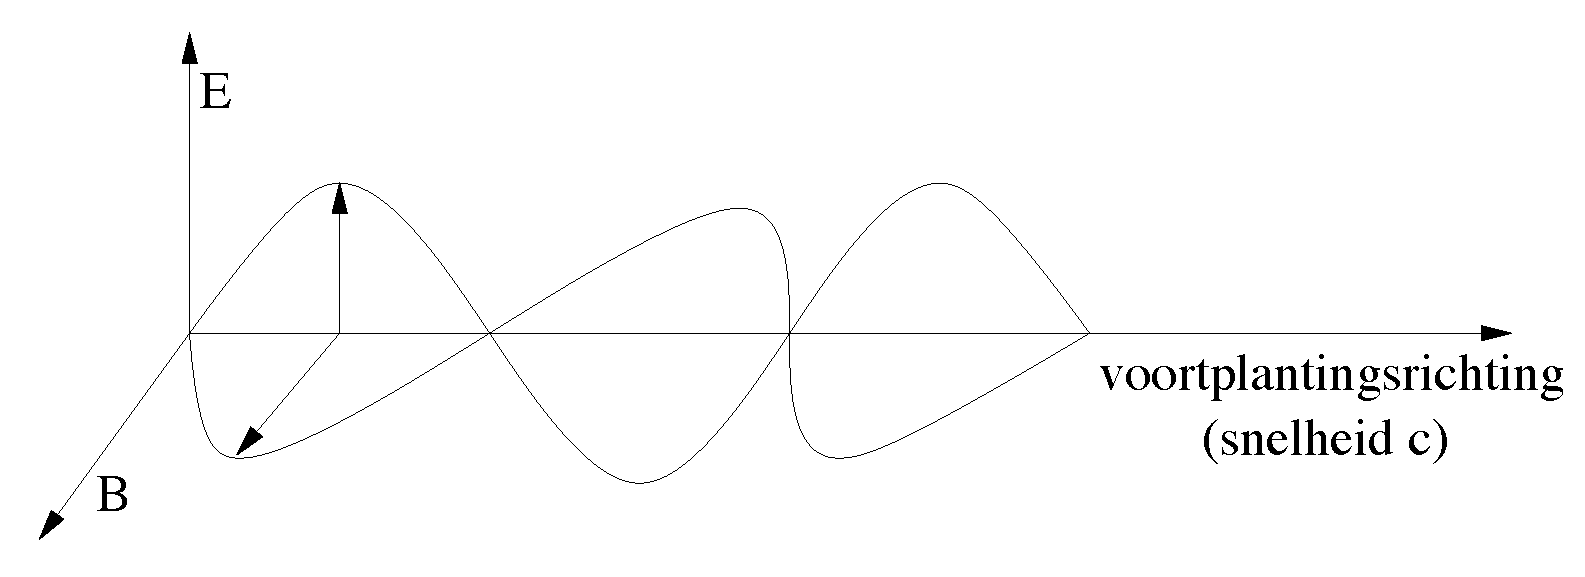
\epsfig{file=emwave.pdf, width=0.7\textwidth}
\caption{{\sl Elektromagnetische golf.}}
\label{f:emgolf1}
\end{figure}

Radiogolven, lichtgolven, R\"{o}ntgenstralen zijn allemaal voorbeelden van 
elektromagnetische golven, allemaal gekarakteriseerd door dezelfde 
voortplantingssnelheid $c$ (waarin verschillen ze?).
De snelheid van het licht in vacu\"um, $c$, is experimenteel exact bepaald op\footnote{Deze waarde defini\"eert de lengte van de meter!}:
\begin{displaymath}
c =  299.792.458  \;\; {\rm m/s} 
\end{displaymath}
\begin{displaymath}
{\rm (ongeveer} \;\; 300.000 \;\; {\rm km/s} = 3 \cdot 10^{8} \;\; {\rm m/s})
\end{displaymath}
De vraag die de natuurkunde zich stelde in de periode v\'{o}\'{o}r
Einstein was: wat is het medium waarin elektromagnetische
golven, zoals lichtgolven, zich bewegen?  Wat golft er nu eigenlijk? 
Het `natuurlijke' co\"{o}rdinatenstelsel om elektromagnetische
verschijnselen te beschrijven is dan het co\"{o}rdinatenstelsel ten
opzichte waarvan dit medium in rust is. Het medium werd als re\"eel
beschouwd, en werd `ether' genoemd.  Zoals Einstein zou laten zien was
dit de verkeerde vraag, de ether bestaat eenvoudigweg niet! 

\subsection{Het Michelson \& Morley-experiment}
Het was Ole Roemer die in 1676 voor het eerst aantoonde dat licht een
eindige snelheid heeft. Hij deduceerde dit door zorgvuldig het
tijdstip bij te houden, waarop de maan Io binnentreedt in de schaduw
van de planeet Jupiter, waar Io in 1,77 dagen omheen loopt.  Door de
situatie tijdens oppositie (waar de aarde tussen zon en Jupiter in
staat) en conjunctie (waar de zon tussen aarde en Jupiter staat - en
we dus Jupiter maar moeizaam kunnen waarnemen) met elkaar te
vergelijken ontdekte Roemer dat er een discrepantie was die verklaard
kon worden door aan te nemen dat het licht er ca. 22 minuten voor
nodig had om de aardbaan te doorkruisen, oftewel een afstand af te
leggen van 2 A.E. (Astronomische Eenheden). Met 1 A.E. de gemiddelde
afstand van de aarde tot de zon, bepaald op ca. 150 miljoen km, kwam
Christiaan Huygens twee jaar later uit op een snelheid van 200.000
km/s.  In feite is de snelheid van het licht ca. 300.000 km/s, zodat
Roemer een systematische fout had (in werkelijkheid heeft het licht 16
\`a 17 minuten nodig om de aardbaan te doorkruisen).  

De eerste serieuze laboratorium-metingen om de snelheid van het licht
te achterhalen stammen uit 1849 en werden uitgevoerd door Fizeau, en
stelde de lichtsnelheid vast op 313.000 m/s.  Ook toonde hij aan dat de
lichtsnelheid in een snelstromende vloeistof, zeg met snelheid $v$ in
de voortplantingsrichting van het licht, {\sl niet} toeneemt tot $c+v$ zoals
op basis van de Galileitransformatie verwacht zou worden.

In een beroemde serie van experimenten in de 19$^{\mathrm{e}}$ eeuw probeerden
Michelson en Morley het bestaan van de ether experimenteel aan te
tonen, door meting van de lichtsnelheid ten opzichte van de ether. De
aarde draait om de zon, dus kan de aarde niet in rust zijn ten
opzichte van dit medium, althans niet gedurende elke dag van het jaar
en waarschijnlijk op geen enkele dag. De beweging van de aarde door de
ether kan gemeten worden door de lichtsnelheid in twee loodrecht op elkaar staande richtingen te vergelijken. 

Stelt u zich namelijk voor dat de hypothese van de ether juist is, d.w.z. er is
een medium ten opzichte waarvan de lichtsnelheid de waarde $c$ heeft,
en dat het relativiteitsprincipe van Einstein {\it niet} juist is. Stel
verder voor dat er een experiment wordt uitgevoerd om de snelheid van
het licht $c_{\oplus}$ op aarde te meten, die met snelheid
$\vec{v}_{\oplus}$ (een vector met lengte $v_{\oplus}$) beweegt ten
opzichte van het medium. Als we de snelheid van het licht meten,
parallel met de snelheid van de aarde $\vec{v}_{\oplus}$, vinden we
$c_{\oplus}=c-v_{\oplus}$ omdat de aarde het licht `achtervolgt'. Als
we de snelheid de andere kant op meten, tegenovergesteld aan de
beweging van de aarde, vinden we daarentegen
$c_{\oplus}=c+v_{\oplus}$. Als we nu de snelheid meten loodrecht op de
beweging, vinden we $c_{\oplus}=\sqrt{c^2-v^2_{\oplus}}$ omdat de
lichtsnelheid de hypotenusa is van een rechthoekige driehoek met
zijden van lengte $c_{\oplus}$ en $v_{\oplus}$. Als de hypothese van het bestaan van de ether correct is, laten deze argumenten zien dat de beweging van de aarde
ten opzichte van de ether gemeten kunnen worden.

\begin{figure}[ht]
\centering
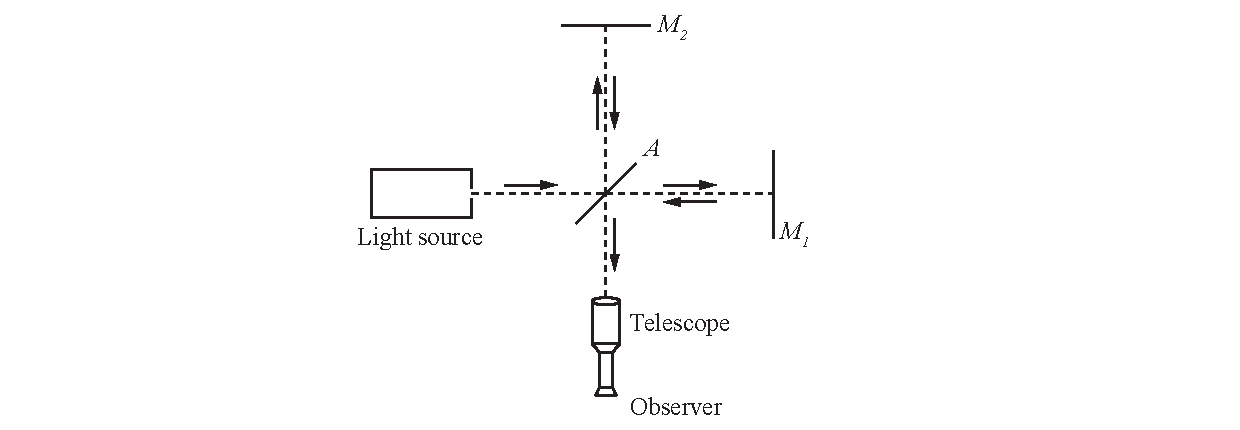
\epsfig{file=MM.pdf, width=\textwidth}
\caption{{\sl Het Michelson \& Morley experiment. Licht uit de `light
source' valt op de halfdoorlaatbare spiegel A. Een gedeelte van het
licht legt het pad via spiegel $M_1$ af, een ander gedeelte een pad
via spiegel $M_2$. In de `telescope' komen de bundels samen en is het interferentiepatroon
zichtbaar.}}
\label{f:mm}
\end{figure}


Het experiment van Michelson \& Morley was ontworpen om deze meting te
verrichten door de lichtsnelheid in twee richtingen loodrecht op elkaar te vergelijken. Omdat het moeilijk is de absolute snelheid te
bepalen, was het experiment ontworpen om de relatieve snelheid van de
twee richtingen te bepalen, met behulp van interferentie van
lichtstralen. In figuur~\ref{f:mm} is het experiment schematisch
weergegeven. Het hele experiment werd gemonteerd op een draaibaar
platform waardoor het gemakkelijk geroteerd kon worden.

Als de totale lengte van elke bundel $l$ is, en een bundel in de
richting parallel met $\vec{v}_{\oplus}$ loopt en de ander daar
loodrecht op, wordt de tijd die het duurt voor het licht om het pad af
te leggen gegeven door:
\begin{equation}
t_{\parallel}=\frac{l}{2(c+v_{\oplus})} +\frac{l}{2(c-v_{\oplus})}
=\frac{lc}{c^2-v^2_{\oplus}}
\end{equation}
omdat de reis van het licht bestaat uit een gedeelte met de stroom mee
en een gedeelte er tegenin. De tijdsduur voor de richting hier
loodrecht op wordt gegeven door
\begin{equation}
t_{\perp} = \frac{l}{\sqrt{c^2-v_{\oplus}^2}}
\end{equation}
omdat deze gehele reis gemaakt wordt loodrecht op de bewegingsrichting. Definieer nu $\beta=v_{\oplus}/c$ en bereken het tijdsverschil tussen de twee paden. We vinden
\begin{equation}
\Delta t = \frac{l}{c}\left[ \frac{1}{1-\beta^2} + \frac{1}{\sqrt{1-\beta^2}}   \right]
\end{equation}
Voor kleine waarden van $x$ geldt $(1+x)^n \sim 1+nx$ en hiermee wordt
\begin{equation}
\Delta t \sim \frac{l}{2c} \beta^2
\end{equation}

Bij een rotatie van het hele apparaat  zal het ene moment de ene arm
parallel aan de bewegingsrichting van de aarde staan, op het andere
moment de andere arm. Bij een draaiing onder een hoek van 90$^o$ wordt het
tijdsverschil tussen de twee armen dus tweemaal $\Delta t$, en dit
verschil moet observeerbaar zijn in het veranderende
interferentiepatroon van de twee lichtbundels. In de opstelling van
Michelson \& Morley zou dit een verschuiving van 0.4 perioden van de
golflengte van het licht moeten opleveren. Echter, er werd geen enkele
verschuiving waargenomen. Ook niet een aantal maanden later, nadat het  experiment is herhaald.

Dit beroemde `nulresultaat' betekende een groot probleem voor de ether
theorie, en leidde tot een aantal speculaties. Bijvoorbeeld, kon het
gebeuren dat de aarde de ether in de baan om de zon `meesleurde'? In
een artikel uit 1904 van Lorentz werd de mogelijkheid geopperd dat
alle bewegende lichamen krimpen in de richting van de beweging, met
een grootte die precies voldoende was om het experimentele
nul-resultaat te verklaren. Al deze idee\"en waren teveel een ad-hoc
oplossing.

De verklaring van Einstein - die zegt dat er helemaal geen ether is en
dat de lichtsnelheid gelijk is voor alle waarnemers - is de verklaring
die stand heeft gehouden. Het Michelson \& Morley experiment was een
poging van de `schipper' om de snelheid van zijn boot te bepalen
zonder uit het raam te kijken of te vergelijken met een ander
voorwerp. Volgens het relativiteitsprincipe waren ze gedoemd te
mislukken.



%%% Local Variables: 
%%% mode: latex
%%% TeX-master: "Galilei"
%%% End: 
         % 26-03-2011 APC - polished plots
\chapter{Tijddilatatie en lengtecontractie}
\vspace{-1cm}\begin{flushright}
{\it `Its not that I am smart, \\it's just that I stay with the problem longer'}\\ A. Einstein
\end{flushright}

We hebben gezien dat Einstein in 1905 een rigoureuze stap zette 
door te postuleren dat er een relativiteitsprincipe moest bestaan dat zowel gold voor
mechanica als voor elektromagnetisme. De twee postulaten waarop de speciale relativiteitstheorie berusten zijn, zoals we eerder zagen
\begin{enumerate}
\item \underline{Het relativiteitsprincipe}\\ De natuurwetten en de
resultaten van alle experimenten uitgevoerd in een zeker
referentiestelsel zijn onafhankelijk van de translatiebeweging van het
systeem\footnote{We gebruiken de woorden referentiestelsel en
co\"{o}rdinatenstelsel door elkaar. De hier bedoelde equivalente
co\"{o}rdinatenstelsels worden ook wel inertiaalstelsels genoemd: dat
zijn dus referentiestelsels waarin dezelfde krachten werken,
c.q. `waarop' geen krachten werken, cf~\ref{v:galilei3}}.  In de
woorden van Einstein: als co\"{o}rdinatenstelsel $S^{'}$ met constante
snelheid rechtlijnig beweegt t.o.v. co\"{o}rdinatenstelsel $S$ dan
verlopen natuurkundige verschijnselen t.o.v. $S^{'}$ volgens precies
dezelfde natuurwetten als t.o.v. $S$.
\item \underline{Constantheid van de lichtsnelheid}\\ De lichtsnelheid
is eindig en {\sl on}afhankelijk van de bewegingstoestand van de lichtbron.
Het is de limietsnelheid voor natuurkundige objecten (in dit tweede
postulaat wordt impliciet aangenomen dat de lichtsnelheid als
fundamentele natuurconstante een universele rol speelt en niet alleen
van belang is voor verschijnselen waar licht bij betrokken is). Met
andere woorden: de lichtsnelheid heeft in ieder inertiaalstelsel
dezelfde waarde.

\end{enumerate}

\section{Synchroniseren van de tijd}
We hebben gezien dat alle beweging in de Newtonse
natuurkunde gebaseerd was op de grondgedachte: het bestaan van een
universele tijd. Maar we zagen dat dit niet langer houdbaar is, en
Einstein voegt toe ``de rechtvaardiging van een natuurkundig concept
is alleen mogelijke in duidelijke relatie met observaties''. 

Hoe meten we tijd? We kunnen de tijd meten aan de hand van een wekker,
een stopwatch, de rotatie van de aarde, de hartslag, etc. We noemen
dit in algemene zin een `klok'. En als we tijd meten, doen we dit altijd 
aan de hand van gelijktijdige gebeurtenissen. Bijvoorbeeld, als we zeggen
dat een trein om 7 uur op het station arriveert, bedoelen we: ``het
moment dat de kleine wijzer van mijn horloge op de 7 staat, 
en het arriveren van de trein, zijn twee gelijktijdige gebeurtenissen''. 

Dit klink triviaal, maar Einstein voorzag het volgende probleem.  Met
een klok kunnen we de snelheid van een voorwerp meten. Daartoe bepalen
we de plaats $\vec{r}_1$ van het voorwerp op tijdstip $t_1$ en de
plaats $\vec{r}_2$ op tijdstip $t_2$. Hiermee wordt de snelheid
\[
v = \frac{\vec{r}_2-\vec{r}_1}{t_2-t_1}.
\]
Maar dit betekent, gezien het bovenstaande, dat we gebruik moeten
maken van het aflezen van de tijd $t_1$ van een klok, op het moment
dat het lichaam op plaats $\vec{r}_1$ passeert, en gebruik maken van
een {\it andere} klok op plaats $\vec{r}_2$ om tijdstip $t_2$ te lezen
wanneer het lichaam in $\vec{r}_2$ arriveert. En welke klok we ook
gebruiken, onze meting van snelheid is zonder betekenis als we niet
zeggen wat we bedoelen met {\it dezelfde} tijd op twee verschillende
locaties. Als we informatie met oneindige snelheid konden versturen,
zou dit geen probleem opleveren. Maar dit is niet het geval; we kunnen
klokken niet beter synchroniseren dan met behulp van de snelheid van
het licht. 

Hoe kan dit synchroniseren in zijn werk gaan? We kunnen twee klokken
plaatsen, een op plaats $r_1$ en de ander op plaats $r_2$. We hebben
hiermee een `tijd op plaats $r_1$', en een `tijd op plaats $r_2$'
gedefini\"eerd. Om een {\it gemeenschappelijke} tijd voor $r_1$ en $r_2$
teweeg te brengen, kunnen we stellen dat de tijd voor een lichtsignaal
om van $r_1$ naar $r_2$ te komen, gelijk is aan die om van $r_2$ terug
naar $r_1$ te komen; zie het tweede postulaat. Nu kunnen we eenvoudig
een spiegel in $r_2$ zetten, en een lichtsignaal vanuit $r_1$ sturen
naar $r_2$, welke gereflecteerd wordt en weer terug komt in
$r_1$. Noem deze tijdsduur $t_0$, en we kunnen {\it defini\"eren} dat
het signaal in $r_2$ aankwam op tijdstip $t_0/2$.  Hiermee is de klok
op plaats $r_2$ gesynchroniseerd met de klok op plaats $r_1$. Dit
kunnen we voor een heel aantal klokken op elke plaats $r_i$ doen, en
zo klokken op elke willekeurige plaats synchroniseren.

\section{Relativiteit van gelijktijdigheid}
De consequentie van Einsteins manier om klokken  te synchroniseren op
verschillende plaatsen is dat {\it gelijktijdigheid} een relatief
begrip wordt, en niet langer absoluut geldig is. Dit kun je zien aan
hand van het volgende voorbeeld.

Stel je hiervoor een lange trein voor, met lengte $L$. Helemaal aan de
kop van de trein, en helemaal aan het einde van de trein, staan twee
klokken die de tijd meten. Een waarnemer die precies midden in de
trein staat, stuurt een lichtflits uit die zowel naar de kop als naar
het einde van de trein gaat. Omdat de lichtsnelheid naar beide kanten
gelijk is, zal deze waarnemer op de trein zeggen dat de klok op de
kop van de trein {\it tegelijkertijd} met de klok aan het einde van de
trein het licht signaal ontvangt. De waarnemer op de trein
zal dus concluderen dat de ontvangst van de lichtflits aan beide zijden van
de trein een {\it gelijktijdige}  gebeurtenis is.

Maar hoe vergaat het de waarnemer op het perron die de trein voorbij
ziet komen? Laten we aannemen dat het midden van de trein net 
langskomt als de lichtflits verstuurd wordt. Omdat de trein rijdt  zal
de flits naar de voorkant van de trein een iets langere
weg moeten afleggen. Dit omdat de trein een stukje verder rijdt gedurende
de tijd dat het licht nodig heeft om naar de klok aan de kop van de
trein te komen. Omgekeerd hoeft het licht een iets kortere weg af te
leggen om het einde van de trein te bereiken, omdat het einde van de
trein iets naar de waarnemer op het perron is toegekomen gedurende de
tijd die het licht nodig heeft om te reizen. Ook voor deze waarnemer
is de snelheid van het licht constant (tweede postulaat!), en hij komt
tot een andere conclusie. Voor hem bereikt de lichtflits het einde
van de trein {\it eerder} dan het licht de kop van de trein bereikt!
Voor hem zijn dit dus geen gelijktijdige gebeurtenissen. Met andere
woorden, dit `gedachtenexperiment' laat zien dat gelijktijdigheid
afhangt van de keuze van het inertiaalsysteem.
Overigens, om een
echt meetbaar verschil te geven met de waarnemer {\it op} de trein,
moet de trein natuurlijk wel met erg hoge snelheid langs het perron razen!

\section{Tijddilatatie} \label{s:lichtklok}
Stel twee waarnemers voor, Dirk (D) en Erika (E), die ten opzichte van
elkaar bewegen in twee ruimteschepen.  D meet de snelheid $v$ van E
ten opzichte van zijn ruststelsel. Als gevolg van de symmetrie van
deze situatie zal ook E een snelheid $v$ meten van de snelheid van D,
ten opzichte van haar ruststelsel. Als dit niet direct duidelijk is, bedenk dan dat 
in dit voorbeeld D en E volledig inwisselbaar zijn. Als D en E  niet dezelfde snelheid zouden meten, zou een van beide in een `speciaal' co\"ordinatenstelsel zitten, en dit is precies in tegenspraak met de postulaten van de relativiteitstheorie.

\begin{figure}[ht]
\centering
%\includegraphics[width=.5\textwidth]{syllabus.pictures/Lichtklok}
\epsfig{file=Lichtklok.pdf, width=0.5\textwidth}
\caption{{\sl Schematische tekening van een lichtklok. De lengte die het licht aflegt tussen lamp en detector is 1 m.}}
\label{f:lichtklok}
\end{figure}

Stel nu voor dat D en E beide een zeer bijzondere klok bij zich
hebben. Deze `licht-klokken' bestaan eenvoudigweg uit een lampje, een
spiegel, een fotodetector en wat elektronica. De fotodetector zit vlak
naast het lampje en de spiegel bevindt zich op 0.5 m hoogte, zie
figuur~\ref{f:lichtklok}. Als de klok gestart wordt gaat het lampje
eventjes aan, een lichtflits kaatst via de spiegel in de
fotodetector. Wanneer de fotodetector het licht registreert, geeft het
een signaal aan het lampje om onmiddellijk een nieuwe lichtflits uit te
zenden. Zo tikken de lichtflitsen met een regelmaat van $1/c \sim 3.3
\times 10^{-9}$ s, oftewel elke 3.3 ns een tik. De lichtsnelheid is
hetzelfde voor alle waarnemers, dus $c$ is hier een conversiefactor
tussen tijd en afstand. Deze lichtklok tikt de tijd in
meters\footnote{Het ISO (International Standard Organization)
defini\"eert zo de meter in termen van seconden. De lichtsnelheid
wordt daarbij {\it gedefini\"eerd} met een waarde $c=2.99792458 \times
10^8$ m s$^{-1}$.}.

Stel nu dat D de klok rechtop houdt, zodanig dat het licht loodrecht op zijn
bewegingsrichting ten opzichte van E kaatst. We hebben gezien dat D zijn klok tikt
met intervallen van 3.3 ns., maar wat ziet E? Merk op dat D beweegt
met een snelheid $v$ ten opzichte van E, dus in het ruststelsel van E
maakt het licht geen echte rondgang. Gedurende de reis van het licht
omhoog naar de spiegel en terug legt D een afstand af in de
loodrechte richting; het pad van het licht wordt een zig-zag, en is
langer dan het rechte op-neer pad bij een stilstaande klok, zie figuur~\ref{f:lichtklok2}.

\begin{figure}[ht]
\centering
%\includegraphics[width=.5\textwidth]{syllabus.pictures/Lichtklok2}
\epsfig{file=Lichtklok2.pdf, width=0.5\textwidth}
\caption{{\sl Het traject van het licht in de klok van waarnemer D zoals
geobserveerd door D (a) en E (b). Merk op dat het traject langer is in
het stelsel van E, en dus meet E een langer tijdsinterval $t'$.}}
\label{f:lichtklok2}
\end{figure}

Toch meten waarnemers dezelfde lichtsnelheid $c$ (het
relativiteitsprincipe!), en moeten we concluderen dat E een groter
tijdsinterval $\Delta t'$ tussen twee tikken meet dan waarnemer D\footnote{Alle grootheden die E meet worden met een accent
weergegeven, de grootheden die D meet zonder accent.}.
 Wat is het verschil tussen $\Delta t$ en $\Delta t'$?

In het stelsel van E, in een tijd $\Delta t'$, beweegt D het stuk
$\Delta x'=v \Delta t'$ naar voren, en legt het licht een afstand
$\Delta l' = c\Delta t'$ af. Volgens Pythagoras is $(\Delta l')^2
=(\Delta x')^2 +(\Delta y')^2$ waarbij $\Delta y'$ de lengte
van het traject in de $y$ richting is.  We zullen later aantonen dat $\Delta y'
= \Delta y$, en is dus 1 m. Omdat in het stelsel van D geldt $\Delta y= \Delta l = c \Delta t$ vinden we
\begin{equation}\label{e:timedil}
\Delta t' = \frac{\Delta t}{\sqrt{1-\frac{v^2}{c^2}}}
\end{equation}
De tijdsintervallen tussen de tikken van de klok van D zijn groter
zoals gemeten door E dan zoals gemeten door D. Dit effect heet {\it
tijddilatatie}. Bewegende klokken lopen langzamer.

In de literatuur wordt vaak de volgende notatie gebruikt. De dimensieloze grootheid $\beta$ staat voor de snelheid, 
\begin{equation}
\beta = \frac{v}{c},
\end{equation}
en omdat niets sneller kan gaan dan de lichtsnelheid $c$, geldt $-1 \leq \beta \leq 1$. De {\it Lorentzfactor} $\gamma$ is gedefinieerd als
\begin{equation}
\gamma = \frac{1}{\sqrt{1-\frac{v^{2}}{c^{2}}}} = \frac{1}{\sqrt{1-\beta^2}}\label{f:gamma}
\end{equation}
Voor deze factor geldt $\gamma \geq 1$. Met deze nieuwe symbolen wordt formule~\ref{e:timedil} geschreven als $\Delta t' = \gamma \Delta t$. 

We hebben nu gevonden dat `bewegende klokken langzaam lopen'. Een punt
van kritiek zou kunnen zijn dat dit alleen is aangetoond voor deze
merkwaardige lichtklokken. Toch kunnen we laten zien dat {\it alle}
klokken onderhevig zijn aan dit dilatatie effect. Stel namelijk voor
dat, naast de lichtklok, waarnemer D ook nog een horloge of een ander
mechanisme heeft om de tijd te meten dat elke 3.3 ns tikt. En stel
voor (hetgeen onjuist is!) dat dit horloge geen tijd-dilatatie effect
ondergaat; dat wil zeggen, stel voor dat E het horloge elke 3.3 ns
ziet tikken ongeacht de snelheid van D. Wanneer D stilstaat ten
opzichte van E tikken het horloge en de lichtklok met dezelfde
snelheid, maar wanneer D met hoge snelheid beweegt beginnen ze
ongelijk te tikken omdat (zoals we veronderstelden) de \'e\'en
tijd-dilatatie heeft en de ander niet. Maar dan kan D uit de relatieve
tik-snelheden van het horloge en de lichtklok achterhalen wat zijn
snelheid is, en zo schendt hij het relativiteitsprincipe. Het is niet
mogelijk de klokken gelijk te laten lopen voor waarnemer D, en ze
ongelijk te laten lopen voor waarnemer E.

Men kan opmerken dat het relativiteitsprincipe al is
geschonden. Immers, als D en E in deze symmetrische situatie zitten,
hoe kan het dan dat E langere tijdsintervallen meet dan D? Welke
intervallen meet D ten opzichte van E? Nu moeten we voorzichtig zijn:
E meet langere intervallen voor de klok van D dan D zelf meet. Door
het relativiteitsprincipe moet het daarom zijn dat D {\it ook} grotere
tijdsduur intervallen meet voor een klok in het ruimtestation van E,
dan E zelf meet. En dit is juist, uiteindelijk kunnen we D en E in de
hele argumentatie verwisselen. Dit is het fundamentele
tegen-intu\"itive karakter van de relativiteitstheorie. Hoe kan het
dat beide waarnemers langzamere tijdsintervallen meten van elkaars
klokken? Feit blijkt dat er helemaal geen tegenspraak in deze bewering
zit zodra we het concept van `absolute tijd' voor alle waarnemers,
waar Newton zo aan hechtte, opgeven.

\subsection{Observatie van tijddilatatie}
In de vorige paragraaf, zoals in de rest van dit college, is het
belangrijk een verschil te maken tussen wat een ideale waarnemer {\it
observeert} en wat een ideale waarnemer {\it ziet}. `Observeren' staat
voor `het meten van echte effecten met de juiste experimentele
technieken', terwijl `zien' is gereserveerd voor schijnbare effecten,
of fenomenen die gerelateerd zijn aan het feit dat we vanuit een
specifiek gezichtspunt kijken met een specifiek paar ogen.

Hoewel E {\it observeert} dat de klok van D langzaam loopt, {\it ziet}
zij wellicht iets heel anders. De tijds intervallen tussen de tikken
van de klok van D die zij ziet, hangen af van het tijddilatatie effect
{\it en} de verandering van de afstand die het licht moet afleggen om
naar E te komen. Deze afstand verandert omdat D beweegt ten opzichte
van E, zie figuur~\ref{f:tijdpad}.

\begin{figure}[ht]
\centering
%\includegraphics[width=.5\textwidth]{syllabus.pictures/Tijdpad}
\epsfig{file=Tijdpad.pdf, width=0.5\textwidth}
\caption{{\sl Observeren van tijddilatatie. Omdat D beweegt ten opzichte
van E, leggen de lichtflitsen ($F_1$ tot $F_4$) van zijn klok
verschillende afstanden ($S_1$ tot $S_4$) af om waarnemer E te
bereiken. Dus de tijd om E te bereiken is verschillend voor de
lichtflitsen. E moet hiervoor corrigeren voordat zij een uitspraak kan
doen over tijddilatatie. Pas nadat deze correcties zijn gemaakt
observeert E de voorspelde tijddilatatie.}}
\label{f:tijdpad}
\end{figure}


U zult ontdekken dat het tijdsinterval tussen twee tikken veel langer
is dan wat tijddilatatie voorspeld, omdat
opeenvolgende flitsen van verder en verder weg moeten komen. Dit effect heet
{\it Doppler-verschuiving} en zal verder in het college behandeld
worden.

\section{Lengtecontractie} \label{s:contractie}
Stel nu dat er twee planeten zijn, A en B, beide in rust ten opzichte van  waarnemer E.
Waarnemer D maakt een reis van A naar B terwijl waarnemer E stilstaat bij een planeet.
Gedurende de reis van D ziet waarnemer E dat er 100 tikken verstrijken op de klok van D.
 
Dan moet D ook zelf 100 tikken zien verstrijken gedurende deze
reis. Immers, het is mogelijk de klok bijvoorbeeld een gaatje te laten
prikken in een kaart elke keer dat het tikt. D kan het prikken laten
beginnen bij planeet A en laten eindigen bij planeet B, en er moeten
dan een bepaald aantal prikken in de kaart zitten. D en E moeten met
elkaar overeenstemmen hoeveel gaatjes er in de kaart zitten; zij
kunnen immers altijd na de reis bij elkaar komen en de gaatjes tellen.

Behalve het aantal gaatjes, zijn ze het ook eens over hun onderlinge
snelheid (ze moeten wel: hun situatie is volledig inwisselbaar - dit
argument is eerder gemaakt). Echter, waar ze het niet met elkaar over
eens zijn is de snelheid waarmee elkaars klokken tikken. E bepaalt de
afstand tussen de planeten A en B als $l'=100 v \Delta t'$. Echter, 
D bepaalt de afstand als $100 v \Delta t = l'/\gamma$. Omdat $\gamma > 1$ meet
D een {\it kortere} afstand dan E.  D beweegt ten opzichte van de
planeten A en B, terwijl E stil staat ten opzichte van deze planeten.
In feite kunnen de planeten A en B gezien worden als de eind-punten
van een heel lange meetlat die waarnemer E vasthoudt; een meetlat die
beweegt ten opzichte van D.  We concluderen dat een bewegende meetlat
korter wordt; dit effect heet lengtecontractie oftewel 
{\it Lorentzcontractie}.

Het is eenvoudig aan te tonen dat deze Lorentzcontractie alleen
optreedt in de richting parallel aan de bewegingsrichting. Immers,
stel dat E en D beide een holle pijp van heel dun materiaal hebben, beide met exact dezelfde diameter, zodat de pijpen niet in elkaar geschoven kunnen worden.
Stel nu dat de ori\"entatie van de pijpen  parallel aan hun onderlinge
bewegingsrichting is. Als we nu aannemen (wat niet juist is!) dat
de diameter van E's pijp anders wordt in het co\"ordinatenstelsel van
D, zou de pijp van D om die van E heen passen. Maar in de omgekeerde situatie zou dan de pijp van D kleiner moeten worden in het co\"ordinatenstelsel van E!
Hier is een contradictie, en we concluderen dat de diameter van de
pijp niet verandert bij beweging loodrecht op deze diameter.

Merk op dat we eerder bij de lichtklok hadden aangenomen dat de
lengte $y$ loodrecht op de beweging niet veranderd van
referentiesysteem naar referentiesysteem. Dit hebben we nu aangetoond.

\section{Niet-relativistische limiet}
We zien dat wanneer $v \ll c$ de Lorentzfactor 
$\gamma = \sqrt{\frac{1}{1-\beta^2}}$ vrijwel gelijk is 
aan $1$ en relativistische effecten geen rol van betekenis spelen (zie Figuur \ref{fig:gammagraf}).
Een voertuig met een lengte van $4$ m dat met $100$ km/uur beweegt, is
$2\cdot 10^{-18}$ m korter dan  wanneer het in rust is.
Dat is $0.2 \%$  van de diameter van een proton...

\begin{figure}[t]
	\centering
%		\includegraphics[width=1.00\textwidth]{syllabus.pictures/gammagraf}
		\epsfig{file=gammagraf.pdf, width=\textwidth}
	\caption{{\sl Grafiek van $\gamma$ uitgezet tegen v/c. Duidelijk te zien is de asymptoot bij de lichtsnelheid, v/c = 1: daar wordt $\gamma \rightarrow \infty$. Tevens is het gedrag bij zeer lage snelheid (v/c $\approx 0$) duidelijk zichtbaar: $\gamma \approx 1$, het klassieke domein.}}
	\label{fig:gammagraf}
\end{figure}


\section{Kosmische stralen}
Onze atmosfeer wordt voortdurend gebombardeerd door kosmische straling.
Kosmische stralen zijn deeltjes van vaak hoge energie die ons uit het heelal 
bereiken, o.a. (in feite voornamelijk) protonen\footnote{Oorsprong, energiespectrum en samenstelling van kosmische stralen 
vormen interessante, nog lang niet opgehelderde onderwerpen van 
wetenschappelijk onderzoek.}. Deze protonen raken stikstof- of zuurstofkernen op grote hoogte, tientallen 
kilometers boven het aardoppervlak, in de bovenste lagen van de atmosfeer. We weten dat bij die botsingen o.a. muonen (symbool voor een muon: $\mu$)
geproduceerd worden. We weten\footnote{Vakgebied : hoge-energiefysica}
ook dat muonen in rust in ons laboratorium een (gemiddelde) levensduur 
hebben van $\tau = 2,2\ \mu$s $= 2,2\cdot  10^{-6}$s.
Volgens de niet-relativistische formule zou een muon, zelfs als het met de 
lichtsnelheid $c$ bewoog, slechts (gemiddeld) een 
afstand $c\tau = 659$ m afleggen.
We nemen de muonen echter op het aardoppervlak waar, dus ze reizen 
pakweg $30$ km.
Dus hun levensduur, gezien door een waarnemer op aarde, is een factor 
$30.000/659$ groter dan de levensduur in het rustsysteem van het muon.
Dus: $\gamma = 30.000/659 = 45.5$ waaruit volgt $v = 0,9998$ c.
De muonen reizen dus vrijwel met de lichtsnelheid en leven dankzij de 
tijddilatatie lang genoeg om de $30$ km te overbruggen.

\section{Tweelingparadox}
De resultaten van de relativiteitstheorie kunnen aanleiding geven tot 
`tegenstellingen' die de theorie ter discussie stellen.
Het gaat hier dan om schijnbare tegenstellingen, paradoxen, die ons er 
alleen maar voor waarschuwen dat de theorie zorgvuldig en correct 
ge\"{i}nterpreteerd dient te worden.
Laten we als voorbeeld nemen: tijddilatatie, 
`bewegende klokken lopen langzamer'.\\
Vanuit $S$ zien we een met $S^{'}$ meebewegende klok langzamer lopen, 
vanuit $S^{'}$ zien we een in $S$ in rust zijnde klok langzamer lopen.\\
Dat lijkt in tegenspraak, wie heeft er nu gelijk, de waarnemer in $S$ of 
die in $S^{'}$?
Natuurlijk hebben ze allebei gelijk en is er geen tegenspraak.
Wanneer we twee klokken willen vergelijken moeten we dat in hetzelfde 
referentiestelsel op dezelfde plaats doen.\\
Indien we de klokken uit het voorbeeld vervangen door leden van een tweeling, 
waarvan er \'{e}\'{e}n op aarde blijft en de ander vertrekt in een ruimteschip 
dan doet zich dezelfde situatie voor: beide nemen waar dat de ander minder 
snel oud wordt en dat is volkomen in orde.
Het `probleem' ontstaat wanneer de ruimtereiziger besluit om huiswaarts te 
keren om de andere helft van de tweeling te bezoeken.
Dan blijkt de ruimtereiziger wel degelijk jonger te zijn.
(Dit is geverifi\"{e}erd met aan boord van vliegtuigen vervoerde nauwkeurige 
klokken.)
Maar: het omkeren van de ruimtereiziger is niet te beschrijven als een 
eenvoudige Lorentztransformatie, anders gezegd: het rustsysteem van de 
ruimtereiziger, $S^{'}$, is geen inertiaalsysteem.
Systeem  $S$ 
is dat wel en daarom is het correct de situatie vanuit $S$ te beschrijven 
en in $S$ is de ruimtereiziger inderdaad langzamer verouderd dan de 
achterblijver.



	% 26-03-2011 APC - polished plots	% + Gamma factor grafiek ingevoegd
\chapter{Lorentztransformatie}
\vspace{-1cm}\begin{flushright}
{\it `Its not that I am smart, \\it's just that I stay with the problem longer'}\\ A. Einstein
\end{flushright}

Het tweede postulaat zoals geformuleerd in het voorgaande hoofdstuk is
duidelijk in tegenspraak met de Galileitransformatie en het is nu onze
taak een transformatie te vinden (het eerste postulaat zegt in feite
dat die er moet zijn) die in overeenstemming is met het tweede
postulaat.  Deze transformatie is in 1905 door Einstein gevonden en is
bekend geworden onder de naam Lorentztransformatie.  De afleiding
ervan is wiskundig gezien zeer eenvoudig, maar vereist, zoals we
zullen zien, nogal wat hersengymnastiek.

\section{Invariante interval}
We hebben gezien dat in de drie-dimensionale ruimte de co\"ordinaten van
twee punten $\vec{p}_1$ en $\vec{p}_2$ voor verschillende waarnemers,
waarvoor de onderlinge referentiesystemen zijn getransleerd, anders
zijn. Ze zijn het in deze drie-dimensionale ruimte wel eens over de
afstand tussen deze twee punten; dit is de invariant $\Delta r$.

We willen nu een dergelijke grootheid vinden voor een paar van `gebeurtenissen', een lengte in
de 3+1 dimensionele ruimte-tijd. Beschouw hiervoor persoon
$A$ die zich in de oorsprong van co\"{o}rdinaten-stelsel $S$ bevindt en
een persoon $B$ in de oorsprong van $S^{'}$.  $S^{'}$ beweegt
t.o.v. $S$ in de positieve $x$-richting met snelheid $v$.  Op $t=0$
valt de oorsprong van $S$ samen met die van $S^{'}$, d.w.z. vallen $A$
en $B$ samen.  Op $t=0$ ontsteekt $A$ heel eventjes een lampje
waardoor zich een bolvormige lichtgolf gaat uitbreiden.  $A$ bevindt
zich in het middelpunt van de bolvormige golf.  Een bol met straal $R$
en de oorsprong van het co\"{o}rdinatenstelsel als middelpunt wordt
beschreven door de formule :
\begin{displaymath}
x^{2} + y^{2} + z^{2} = R^{2}(t)
\end{displaymath}

% \begin{figure}[h]
% \begin{center}
% \mbox{\epsfxsize=8cm\epsffile{syllabus.pictures/spheres.eps}}
% \caption{Bolvormige lichtgolf}
% \label{f:lorentz1}
% \end{center}
% \end{figure}

\begin{figure}[ht]
\centering
%\includegraphics[width=1.00\textwidth]{syllabus.pictures/bolgolf}
\epsfig{file=bolgolf.pdf, width=\textwidth}
\caption{{\sl Bolvormige lichtgolf}}
\label{f:lorentz1}
\end{figure}


Voor een lichtgolf die zich uitbreidt met snelheid $c$ geldt na een tijd $t$: 
$R = ct$ en dus :
\begin{displaymath}
x^{2} + y^{2} + z^{2} = c^{2}t^{2}
\end{displaymath}
oftewel
\begin{equation}
\label{v:lorentz0a}
c^2 t^2 - x^{2} - y^{2} - z^{2} = 0
\end{equation}
Precies dezelfde redenering kunnen we echter volgen voor persoon $B$.
Ook $B$ denkt zich in het midden van de bolvormige lichtgolf te bevinden, het 
tweede postulaat zegt immers dat ook voor B het licht zich met snelheid $c$ 
uitbreidt.
Voor $B$, dus t.o.v. $S^{'}$, geldt nu geheel in analogie met hierboven :
\begin{displaymath}
x'^{2} + y'^{2} + z'^{2} = c^{2}t'^{2}
\end{displaymath}
oftewel
\begin{equation}
\label{v:lorentz0b}
c t'^2 - x'^{2} - y'^{2} - z'^{2} = 0
\end{equation}
In ons specifieke voorbeeld (beweging in de $x$-richting), geldt 
$(x \neq x^{'},$\newline $y = y^{'}, z = z^{'})$ dus moeten we wel concluderen 
$t \neq t^{'}$ (Aftrekken van \ref{v:lorentz0a} en \ref{v:lorentz0b} levert
$x^{2} - x'^{2} = c^{2}(t^{2} - t'^{2})$ en dus $t^{2} - t'^{2} \neq 0$) .
We komen al snel tot de conclusie dat de tijd voor $B$ anders 
verloopt dan voor $A$.\\
Bij elk referentiestelsel hoort niet alleen een eigen plaatsmeting maar 
ook een eigen tijdmeting.
Hoe plaats en tijd van een bepaald natuurkundig verschijnsel zoals geldend 
in $S$ worden uitgedrukt in plaats en tijd van hetzelfde verschijnsel 
t.o.v. $S^{'}$ wordt gegeven door de Lorentztransformatie.

In elk geval weten we al (zie boven) dat zal moeten gelden:
\begin{equation}
\label{v:lorentz1}
c^2 t'^2 - x'^{^{2}} - y'^{^{2}} - z'^{^{2}} = c^2 t^2 - x^{2} - y^{2} - z^{2} 
\end{equation}
We zeggen dat de grootheid $c^2 t^2 - x^{2} - y^{2} - z^{2}$
{\sl invariant} is onder Lorentztransformaties. 

Iets algemener kunnen we twee gebeurtenissen A en B in het stelsel $S$ beschouwen, met onderling tijdsverschil $\Delta t$ en
ruimteverschillen $(\Delta x,\Delta y, \Delta z)$. We hebben laten zien dat de afstand tussen deze twee gebeurtenissen,
gedefinieerd als 
\begin{eqnarray}
(\Delta s)^2 & \equiv & (c \Delta t)^2 - (\Delta r)^2 \\
             & \equiv & (c \Delta t)^2 - (\Delta x)^2 - (\Delta y)^2 - (\Delta z)^2
\end{eqnarray}
{\it invariant} is onder het relativiteitsprincipe van Einstein.
Dit invariante interval staat centraal in de speciale relativiteitstheorie.

\subsection{Nogmaals de lichtklok}
In paragraaf~\ref{s:lichtklok} hebben we de lichtklok
ge\"introduceerd. In het referentiesysteem van D waarin de klok stil staat, tikte de klok met
tikken van $(c\Delta t)=1$ m (elke 3.3 ns), en de afgelegde afstand in de $x$-richting tussen twee tikken is $\Delta
x=0$. Het invariante interval tussen twee tikken wordt daarmee $(\Delta
s)^2 = (c \Delta t)^2-(\Delta x)^2 = 1 $m$^2$. 

In het referentiestelsel
van E is $c \Delta t' = \gamma$(1 m) en de afgelegde afstand afstand in $x$ tussen twee tikken wordt
gegeven door de snelheid $v$ te vermenigvuldigen met de het tijdsverschil $\Delta t'$, $\Delta x' = \gamma v$(1 m)$/c$. Het
interval in E's referentiesysteem wordt hiermee $(\Delta s')^2
=\gamma^2(1-v^2/c^2)$(1 m$^2$). Omdat geldt dat $\gamma\equiv
1/\sqrt{(1-v^2/c^2)}$, wordt het interval hiermee $(\Delta s')^2 =
(\Delta s)^2 = 1$ m$^2$. We hebben laten zien dat het interval
dezelfde waarde heeft voor waarnemer D en waarnemer E. Voor elke
andere waarnemer die in een referentiesysteem zit, geldt dat hij
andere tijdverschillen meet, en andere ruimte afstanden vindt. Maar het
interval $(\Delta s)^2$ blijft altijd 1 m$^2$.

\section{De eigentijd en eigenlengte}
De {\sl eigentijd} $\Delta \tau$ tussen twee gebeurtenissen is het
tijdsinterval zoals waargenomen in een co\"ordinatenstelsel waarin de
twee gebeurtenissen op dezelfde positie plaatsvinden. Dit is niet in
alle gevallen mogelijk.  Zoals in bovenstaand voorbeeld duidelijk is
gemaakt, is het invariante interval tussen twee gebeurtenissen $c$
maal de eigentijd, of $c\Delta \tau = \sqrt{(\Delta s)^2}$. De
eigentijd is het tijdsinterval in het co\"ordinatenstelsel van D, het
stelsel waarin de lichtklok stil staat. De eigentijd is de tijd zoals
die verloopt voor de waarnemer zelf; het is zijn {\it eigen} tijd.


 Als het interval positief is, is er altijd een co\"ordinatenstelsel te
vinden waarin de positie van de gebeurtenissen hetzelfde is. Dit omdat
een positief interval betekent $|c \Delta t | > | \Delta r|$, dus een
referentiesysteem dat beweegt met een snelheid $\vec{v}=(\Delta
\vec{r})/(\Delta t)$ transformeert  de gebeurtenissen naar hetzelfde punt. En 
de  snelheid is kleiner dan die van het licht. 

Als het interval tussen twee gebeurtenissen kleiner is dan nul, d.w.z.
$(\Delta s)^2 < 0$, is het nog steeds een invariant. Maar er kan in dit
geval geen co\"ordinatenstelsel gevonden worden waarin beide
gebeurtenissen op dezelfde positie plaatsvinden. Dit
co\"ordinatenstelsel is er niet - het zou sneller dan met de lichtsnelheid
moeten bewegen ten opzichte van het stelsel van de twee
gebeurtenissen. Soms wordt hiervoor de {\it eigenlengte} ge\"introduceerd, $\Delta \lambda$, als
de ruimtelijke afstand tussen twee gebeurtenissen in een referentiesysteem waarin de gebeurtenissen
gelijktijdig plaatsvinden. Dit kan alleen als het interval negatief is, en de eigenlengte wordt
dan $\Delta \lambda = \sqrt{|(\Delta s)^2|}$. 

Het interval $(\Delta s)^2$ kan natuurlijk ook precies gelijk zijn
aan nul. Dit is het geval wanneer $(c \Delta t)^2 = (\Delta r)^2$,
met andere woorden, wanneer de wereldlijn overeenkomt met die van het
licht. Omdat de lichtsnelheid in elk co\"ordinatenstelsel dezelfde is,
is dit interval weer gelijk aan nul in elk co\"ordinatenstelsel.

Intervallen $(\Delta s)^2=0$ noemen we {\sl `lichtachtig'}. Intervallen $(\Delta s)^2>0$ noemen we {\sl `tijdachtig'} en
intervallen $(\Delta s)^2< 0$ noemen we {\sl `ruimteachtig'}. Deze intervallen hebben verschillende eigenschappen
met betrekking tot causaliteit; we komen hier op terug.



\section{De Lorentztransformatie, een eenvoudige afleiding}
We defini\"{e}ren co\"{o}rdinatenstelsels $S$ en $S^{'}$ weer als voorheen:
$S^{'}$ beweegt t.o.v. $S$ met constante snelheid $v$ in de positieve 
$x$-richting.
Op $t = t^{'} = 0$ valt de oorsprong van $S$ samen met die van $S^{'}$.
Een lichtflits, uitgezonden in de positieve $x$-richting, bevindt zich op 
plaats $x = ct$, d.w.z. $x - ct = 0$.
T.o.v. $S^{'}$ geldt $x' - ct^{'} = 0$ (zelfde $c$, tweede postulaat!).
Aan beide vergelijkingen wordt voldaan als geldt:
\begin{equation}
x^{'} - ct^{'} = \lambda (x - ct)
\end{equation}
waar $\lambda$ een constante is die we nog moeten bepalen.
We kunnen uiteraard dezelfde redenering volgen voor een lichtflits die wordt 
uitgezonden in de negatieve $x$-richting.
Dan vinden we dat moet gelden:
\begin{equation}
\label{v:lorentz2}
x^{'} + ct^{'} = \mu (x + ct)
\end{equation}
Ook $\mu$ is een nog nader te bepalen constante.
Optellen resp. aftrekken van \ref{v:lorentz1} en \ref{v:lorentz2} levert:
\begin{displaymath}
ct^{'} = \frac{\lambda + \mu}{2} ct - \frac{\lambda - \mu}{2} x \\
\end{displaymath}
\begin{displaymath}
x^{'} = \frac{\lambda + \mu}{2} x - \frac{\lambda - \mu}{2} ct 
\end{displaymath}
We defini\"{e}ren twee nieuwe constanten, $a = \frac{\lambda + \mu}{2}$
en $b = \frac{\lambda - \mu}{2}$ en verkrijgen de overzichtelijke 
vergelijkingen:
\begin{equation}
\label{v:lorentz4}
ct^{'} = act - bx
\end{equation}
\begin{equation}
\label{v:lorentz3}
x^{'} = ax - bct
\end{equation}
waar we nog steeds als taak hebben om $a$ en $b$ te bepalen (d.w.z. uit te 
drukken in $v$, de parameter die de transformatie defini\"{e}ert.)

Voor de oorsprong van $S^{'}$ geldt t.o.v. $S$:
\begin{displaymath}
x = vt
\end{displaymath}
en t.o.v. $S^{'}$ uiteraard:
\begin{displaymath}
x^{'} = 0
\end{displaymath}
Invullen in \ref{v:lorentz3} levert dan dat moet gelden:
\begin{equation}
\label{v:lorentz5}
v = \frac{b}{a}c
\end{equation}

% \begin{figure}
% \begin{center}
% \mbox{\epsfxsize=8cm\epsffile{syllabus.pictures/ruler.eps}}
% \caption{Meetlat}
% \label{f:lorentz2}
% \end{center}
% \end{figure}

\begin{figure}[ht]
\centering
\epsfig{file=ruler.pdf, width=0.5\textwidth}
%\includegraphics[width=.5\textwidth]{syllabus.pictures/ruler}
\caption{Meetlat}
\label{f:lorentz2}
\end{figure}


Nu gebruiken we het relativiteitsprincipe in de volgende redenering: 
een meetlat die langs de $x^{'}$-as ligt, in rust t.o.v. $S^{'}$, 
heeft, gezien vanuit $S$ dezelfde lengte als diezelfde meetlat, gelegen 
langs de $x$-as, in rust t.o.v. $S$, gezien vanuit $S^{'}$!
\begin{itemize}
\item \underline{Observatie 1} \\
Op een zekere tijd $t$ in $S$ kunnen we dus de lengte van de meetlat 
t.o.v. $S^{'}$ bepalen, bijvoorbeeld op \underline{$t = 0$}.
We vinden dan met behulp van \ref{v:lorentz3}:
\begin{displaymath}
x^{'} = ax
\end{displaymath}
\item \underline{Observatie 2} \\
Omgekeerd vinden we op \underline{$t^{'} = 0$}, m.b.v. \ref{v:lorentz3} en 
\ref{v:lorentz4} en gebruikmakend van \ref{v:lorentz5}:
\begin{displaymath}
x^{'} = a(1 - \frac{v^{2}}{c^{2}})x
\end{displaymath}
\end{itemize}
Wanneer we zeggen dat de lengte van de meetlat $l_0$ is, dan bedoelen we: 
de lengte is $l_{0}$ in het systeem waarin de meetlat in rust is.
Observatie 1 (meetlat in rust in  $S^{'}$ gefotografeerd vanuit $S$) leert dan:
\begin{displaymath}
l_{0} = al
\end{displaymath}
waar $l$ dus de lengte t.o.v. $S$ is, d.w.z. ten opzichte van het 
co\"{o}rdinatenstelsel waarin de lat beweegt.
Observatie 2 ($S$ gefotografeerd vanuit $S^{'}$) levert op:
\begin{displaymath}
l = a(1-\frac{v^{2}}{c^{2}})l_{0}
\end{displaymath}
Het combineren van deze resultaten levert dan het volgende resultaat op:
\begin{displaymath}
a = \frac{1}{\sqrt{1-\frac{v^{2}}{c^{2}}}}
\end{displaymath}
Degenen die achterdochtig worden van deze nogal veel woorden kostende 
afleiding vinden de volgende beschouwing misschien eleganter.\\
We pikken de afleiding op na formule \ref{v:lorentz5} en schrijven 
\ref{v:lorentz3} en \ref{v:lorentz4} als :
\begin{equation}
\label{v:lorentz7}
ct^{'} = a(ct - \frac{v}{c}x)
\end{equation}
\begin{equation}
\label{v:lorentz6}
x^{'} = a(x - vt)
\end{equation}
Bovenstaande transformatie geldt als $S^{'}$ beweegt in de positieve 
$x$-richting, dus met snelheid $+v$, t.o.v. $S$.
Maar we kunnen ook $S^{'}$ als rustsysteem kiezen en $S$ als het bewegende 
systeem zien dat t.o.v. $S^{'}$ naar links beweegt, d.w.z. met snelheid $-v$.
De {\sl inverse} transformatie wordt dan onmiddellijk uit de bovenstaande 
verkregen door `accenten te verwisselen' (de accenten slaan immers op het 
bewegende systeem en die rol wordt nu 
overgenomen door $S$) en door $v$ te vervangen door $-v$. 
Dit levert:
\begin{equation}
ct = a(ct^{'} + \frac{v}{c}x^{'})
\label{v:lorentz9}
\end{equation}
\begin{equation}
\label{v:lorentz8}
x = a(x^{'} + vt^{'})
\end{equation}
(Merk op dat deze redenering alleen correct is als $a$ ongevoelig is voor 
het teken van $v$. 
Gelukkig blijkt dat zo te zijn volgens het eerste postulaat.)
Indien we \ref{v:lorentz8} en \ref{v:lorentz9} gebruiken om $t^{'}$ in $t$ 
en $x$ uit te drukken en het resultaat vervolgens vergelijken met 
\ref{v:lorentz7} vinden we 
\begin{displaymath}
a = \frac{1}{\sqrt{1 - \frac{v^{2}}{c^{2}}}}
\end{displaymath}
Aldus hebben we de Lorentztransformatie gevonden:
\begin{displaymath}
ct^{'} = \frac{ct - x \frac{v}{c}}{\sqrt{1 - \frac{v^{2}}{c^{2}}}}
\end{displaymath}
\begin{displaymath}
x^{'} = \frac{x - vt}{\sqrt{1 - \frac{v^{2}}{c^{2}}}}
\end{displaymath}
In ons specifieke geval, relatieve beweging langs de $x$-as, geldt verder
\begin{displaymath}
y^{'} = y
\end{displaymath}
\begin{displaymath}
z^{'} = z
\end{displaymath}
Ga nu na dat formule \ref{v:lorentz1} inderdaad klopt, dat wil zeggen, dat het inderdaad het `invariante interval' $(\Delta s)^2$ invariant laat! Samenvattend:
\begin{quote}
Lorentztransformaties verbinden, net als Galileitransformaties,
inertiaalsystemen op een manier die in overeenstemming is met het
relativiteitsprincipe en het lichtpostulaat. In tegenstelling tot
Galileitransformaties laten ze de lichtsnelheid invariant. Hiermee
zijn ze in overeenstemming met de Maxwell-theorie van het
elektromagnetisme.
\end{quote}

\subsection{Notatie}
We hadden al ingevoerd dat 
\begin{eqnarray}
\beta & = & \frac{v}{c} \\
\gamma & = & \frac{1}{\sqrt{1-\beta^2}}
\end{eqnarray}
De Lorentztransformatie langs de $x$-as wordt hiermee geschreven als:
\begin{eqnarray}
\label{v:lorentz11}
ct' &  = & \gamma (ct - \beta x) \\ \label{v:lorentz10}
x'  &  = & \gamma (x -  \beta ct)\\
y'  & = & y \\
z' & = & z 
\end{eqnarray}
oftewel in matrix vorm\footnote{Voor een overzicht van matrix algebra wordt u doorverwezen naar
de cursus lineare algebra. Kortweg geldt dat een kolom-vector vermenigvuldigd met een matrix een nieuwe kolom-vector oplevert volgens de regel
\[
\left( \begin{array}{c} y_0 \\ y_1 \\ y_2 \\ y_3 \end{array} \right) =
\left( \begin{array}{cccc} a_{00} & a_{01} & a_{02} & a_{03} \\ 
                           a_{10} & a_{11} & a_{12} & a_{13} \\ 
                           a_{20} & a_{21} & a_{22} & a_{23} \\ 
                           a_{30} & a_{31} & a_{32} & a_{33} \end{array} \right) 
\left( \begin{array}{c} x_0 \\ x_1 \\ x_2 \\ x_3 \end{array} \right) =
\left( \begin{array}{c} a_{00} x_0 + a_{01} x_1 + a_{02} x_2 + a_{03} x_3 \\ 
                        a_{10} x_0 + a_{11} x_1 + a_{12} x_2 + a_{13} x_3 \\ 
                        a_{20} x_0 + a_{21} x_1 + a_{22} x_2 + a_{23} x_3 \\ 
                        a_{30} x_0 + a_{31} x_1 + a_{32} x_2 + a_{33} x_3  \end{array} \right). 
\]}.
\begin{equation}
\left( \begin{array}{c} ct' \\ x' \\ y' \\ z' \end{array} \right) =
\left( \begin{array}{cccc} \gamma & -\gamma \beta & 0 & 0  \\ -\gamma\beta & \gamma & 0 & 0  \\ 0 & 0 & 1 & 0  \\ 0 & 0 & 0 & 1 
\end{array} \right) 
\left( \begin{array}{c} ct \\ x \\ y \\ z \end{array} \right) 
\end{equation}
De inverse Lorentztransformatie wordt dan 
\begin{equation}\label{v:lorentz12}
\left( \begin{array}{c} ct \\ x \\ y \\ z \end{array} \right) =
\left( \begin{array}{cccc} \gamma & \gamma \beta & 0 & 0  \\ \gamma\beta & \gamma & 0 & 0  \\ 0 & 0 & 1 & 0  \\ 0 & 0 & 0 & 1 
\end{array} \right) 
\left( \begin{array}{c} ct' \\ x' \\ y' \\ z' \end{array} \right) 
\end{equation}
De ruimte-tijd symmetrie, d.w.z. de verwevenheid van $x$ en $ct$, de 
volstrekt gelijkwaardige rol van beide grootheden, is in deze notatie heel 
duidelijk.

\section{Lorentztransformaties}
De Lorentztransformaties (LT) zijn belangrijk en verdienen een
discussie. De LT transformeren de afstanden $(c\Delta t, \Delta x,
\Delta y, \Delta z)$ tussen de co\"ordinaten van twee gebeurtenissen in
een co\"ordinatenstelsel naar de afstanden $(c\Delta t', \Delta x',$ $
\Delta y', \Delta z')$ in een ander co\"ordinatenstelsel. Het betekent
dat als de LT direct op de co\"ordinaten van \'e\'en gebeurtenis
toegepast worden, impliciet de andere gebeurtenis op co\"ordinaten
$(0,0,0,0)$ in beide stelsels wordt genomen. De transformaties waarbij
de snelheid van een co\"ordinatensysteem anders wordt, noemen we een
{\it boost}. Deze boost-transformaties vormen het hart van de speciale
relativiteitstheorie.

We kunnen eenvoudig de consistentie van de LT laten zien door eerst een
co\"ordinatensysteem te transformeren met snelheid $v$, en vervolgens
weer terug te transformeren met snelheid $-v$. We zullen uiteindelijk
datgene weer terug moeten vinden met waarmee we begonnen waren. Met
andere woorden: LT's met gelijke maar tegengestelde
snelheden moeten elkaars {\sl inverse} zijn. Als we van richting
veranderen, d.w.z. $v\rightarrow -v$, dan wordt $\beta \rightarrow
-\beta$ en $\gamma \rightarrow \gamma$. De transformatie van de
co\"ordinaten $(ct,x)$ naar $(ct',x')$ en weer terug naar co\"ordinaten
$(ct'',x'')$ wordt dan
\begin{eqnarray} 
ct'' & = & \gamma ct' + \beta \gamma x' \\ \nonumber
     & = & \gamma ( \gamma ct -\beta \gamma x) + \beta \gamma (-\beta \gamma ct + \gamma x) \\ \nonumber
     & = & \gamma^2 (ct-\beta x - \beta^2 ct + \beta x)\\ \nonumber
     & = & \gamma^2 (1-\beta^2) ct \\ \nonumber
     & = & ct \\
x'' & = & \beta \gamma ct' + \gamma x' \\ \nonumber
     & = & \beta \gamma ( \gamma ct -\beta \gamma x) + \gamma (-\beta \gamma ct + \gamma x) \\\nonumber
     & = & \gamma^2 (\beta ct-\beta^2 x - \beta ct + x)\\\nonumber
     & = & \gamma^2 (1-\beta^2) x \\\nonumber
     & = & x 
\end{eqnarray}
dus is inderdaad de transformatie langs snelheid $-v$ de inverse van de transformatie langs $v$.

De groep van alle LT's bevat alle lineare transformaties die het interval $(\Delta s)^2$ 
invariant laat. Dit betekent dat ook rotaties in de ruimte, zonder `boost', bij de LT's horen. De
rotatie om de $z$-as met hoek $\theta$ is een voorbeeld:
\begin{equation}
\left( \begin{array}{cccc} 
    1 & 0 & 0 & 0 \\
    0 & \cos\theta & -\sin\theta & 0 \\
    1 & -\sin\theta & \cos\theta & 0 \\
    0 & 0 & 0 & 1 \end{array} \right)
\end{equation}

De LT's bevatten ook de `boost' translaties tussen twee co\"ordinatenstelsels $S$ en $S'$ langs
 willekeurige richting $\vec{v}=(v_x,v_y,v_z)$. 
Zonder verdere afleiding geven we het resultaat
\begin{equation}
\left( \begin{array}{cccc} 
    \gamma & -\gamma\beta_x & -\gamma\beta_y & -\gamma\beta_z \\
    -\gamma\beta_x & 1+\frac{(\gamma-1)\beta_x^2}{\beta^2} & 1+\frac{(\gamma-1)\beta_x\beta_y}{\beta^2} & 1+\frac{(\gamma-1)\beta_x\beta_z}{\beta^2} \\
    -\gamma\beta_y & 1+\frac{(\gamma-1)\beta_x\beta_y}{\beta^2} & 1+\frac{(\gamma-1)\beta_y^2}{\beta^2} & 1+\frac{(\gamma-1)\beta_y\beta_z}{\beta^2}\\
    -\gamma\beta_z & 1+\frac{(\gamma-1)\beta_x\beta_z}{\beta^2} & 1+\frac{(\gamma-1)\beta_y\beta_z}{\beta^2} & 1+\frac{(\gamma-1)\beta_z^2}{\beta^2}
 \end{array} \right)
\end{equation}
waarbij
\begin{eqnarray}
\beta_x & = & v_x/c \\ \nonumber
\beta_y & = & v_y/c \\ \nonumber
\beta_z & = & v_z/c \\ \nonumber
\beta^2 & = & \beta_x^2 + \beta_y^2 + \beta_z^2 \\\nonumber
\gamma & = & (1-\beta_x^2-\beta_y^2-\beta_z^2)^{-1/2}.\nonumber
\end{eqnarray}
Samenstellingen van verschillende LT's zijn zelf ook weer LT's.



\section{Lorentzcontractie}
In paragraaf~\ref{s:contractie} hebben we laten zien dat bewegende
stokken korter worden. We zullen dit nu nogmaals laten zien, maar nu
maken we gebruik van de Lorentztransformatie voor de afleiding van het
resultaat. 

Daartoe bekijken we een bewegende stok. De stok
heeft t.o.v. het co\"{o}rdinatenstelsel waarin hij in rust is een
lengte $l_{0}$.  Wat is dan de lengte t.o.v. het
co\"{o}rdinatenstel-sel waarin hij beweegt?  Wij nemen een stok die
langs de $x^{'}$-as ligt, met het linker uiteinde in de oorsprong van
$S^{'}$ en die in rust is t.o.v. $S^{'}$.  Voor de
$x^{'}$-co\"{o}rdinaat van het rechter uiteinde geldt dus:
\begin{displaymath}
x^{'}_{R} = l_{0}
\end{displaymath}
en voor het linker uiteinde geldt:
\begin{displaymath}
x^{'}_{L} = 0
\end{displaymath}
De overeenkomstige $x$-co\"{o}rdinaten in $S$ volgen uit \ref{v:lorentz12}:
\begin{displaymath}
x_{R} = \gamma (l_{0} + \beta ct^{'}_{R})
\end{displaymath}
\begin{displaymath}
x_{L} = \gamma \beta ct^{'}_{L}
\end{displaymath}
De lengte $l$ t.o.v. $S$ is:
\begin{displaymath}
l = x_{R} - x_{L}
\end{displaymath}
\begin{equation}
\label{v:vier2}
l = \gamma \{l_{0} + \beta c(t^{'}_{R} - t^{'}_{L})\}
\end{equation}
Het is heel belangrijk dat we ons realiseren dat de lengte $l$ t.o.v. $S$ 
gelijk is aan $x_{R} - x_{L}$, waar $x_{R}$ en $x_{L}$ op 
{\sl dezelfde tijd t.o.v. $S$} bepaald worden, 
dus $t_{R} = t_{L}$.
Met behulp van \ref{v:lorentz11} volgt dan:
\begin{displaymath}
ct^{'}_{R} = \gamma (ct_{R} - \beta x_{R})
\end{displaymath}
\begin{displaymath}
ct^{'}_{L} = \gamma (ct_{L} - \beta x_{L}) 
\end{displaymath}
Aftrekken van de vergelijkingen levert:
\begin{displaymath}
c(t^{'}_{R} - t^{'}_{L}) = -\gamma \beta (x_{R} - x_{L}) = -\gamma \beta l
\end{displaymath}
Dit resultaat vullen we in in \ref{v:vier2} en we vinden:
\begin{displaymath}
l = \gamma (l_{0} - \gamma \beta ^{2} l)
\end{displaymath}
\begin{displaymath}
l (1 + \beta ^{2} \gamma ^{2}) = \gamma l_{0}
\end{displaymath}
Aangezien $\gamma ^{2} = \frac{1}{1 - \beta ^{2}}$ (definitie) volgt nu:
\begin{equation}
\label{v:vier3}
l = \frac{l_{0}}{\gamma}
\end{equation}
$l$ is dus kleiner dan $l_{0}$: de bewegende stok is korter, precies
zoals we al eerder gevonden hadden. Dit effect gaat onder de naam {\sl
Lorentzcontractie}.

\section{Optellen van snelheden}
We kunnen nu de juiste formule afleiden voor het optellen van
snelheden, zoals we in de inleiding al bespraken.  Als A met een
snelheid $+u$ in de $x$-richting beweegt ten opzichte van B, en A
gooit een appel met snelheid $+v$ in de $x$-richting ten opzichte van
zichzelf, met welke snelheid ziet dan waarnemer B de appel voorbij
vliegen?  We hadden al gezien dat het klassieke antwoord $w=u+v$
onjuist is. Het juiste antwoord kan worden afgeleid met behulp van de
Lorentztransformaties. Noem hiervoor het moment waarop A de appel gooit $T$, en neem dit als de
 oorsprong van beide co\"ordinatenstelsels, zodat $(ct_T,x_T)=(ct'_T,x'_T)=(0,0)$, waarbij
het stelsel van A aangegeven wordt met accenten. Stel nu verder voor dat een tijdje $t'$ later in het co\"ordinatenstelsel
van A de appel explodeert. De co\"ordinaten van de explosie worden hiermee $(ct',vt')$ in het stelsel van A.
In het co\"ordinatenstelsel in rust ten opzichte van B vind gebeurtenis $T$ ook plaats in de oorsprong, en de
explosie van de appel vind plaats met co\"ordinaten verkregen uit de Lorentztransformatie:
\begin{eqnarray}
ct & = & \gamma c t' + \beta \gamma vt' \\ \nonumber
x & = & \beta \gamma c t' + \gamma vt'
\end{eqnarray}
De snelheid $w$ zoals B die meet is eenvoudigweg $x/t$ oftewel
\begin{eqnarray}
w &=& c\frac{\beta\gamma c t'+\gamma v t'}{\gamma c t'+\beta \gamma vt'} \\\nonumber
 &=& \frac{u+v}{1+uv/c^2}
\end{eqnarray}
en is dus kleiner dan $u+v$.


We gaan nu hetzelfde resultaat opnieuw afleiden, maar dan iets
formeler. We zullen daarbij vinden dat bij een translatie langs de
$x$-as niet alleen de formule voor het optellen van snelheid in de
$x$-richting, maar ook in de $y$- en $z$-richting moet worden
aangepast.

Per definitie geldt voor de snelheid:
\begin{displaymath}
V'_{x} = \frac{dx'}{dt'}
\end{displaymath}
Vul nu in (formule \ref{v:lorentz10}):
\begin{displaymath}
x' = \gamma (x - \beta ct)
\end{displaymath}
dan vinden we:
\begin{displaymath}
V'_{x} = \gamma \frac{dx}{dt'} - \beta \gamma c \frac{dt}{dt'}
\end{displaymath}
Verder geldt (`kettingregel'):
\begin{displaymath}
\frac{dx}{dt'} = \frac{dx}{dt} \frac{dt}{dt'}
\end{displaymath}
en dus vinden we:
\begin{displaymath}
V'_{x} = (\gamma \frac{dx}{dt} - \beta \gamma c)\frac{dt}{dt'}
\end{displaymath}
en aangezien
\begin{displaymath}
V_{x} = \frac{dx}{dt}
\end{displaymath}
wordt dit
\begin{equation}
\label{v:optel1}
V'_{x} = (\gamma V_{x} - \beta \gamma c)\frac{dt}{dt'}
\end{equation}
Nu gebruiken we (formule \ref{v:lorentz12}):
\begin{displaymath}
ct = \gamma (ct' + \beta x')
\end{displaymath}
waaruit volgt:
\begin{displaymath}
\frac{dt}{dt'}  = \gamma + \frac{\beta \gamma}{c} V'_{x}
\end{displaymath}
invullen hiervan in formule \ref{v:optel1} levert dan:
\begin{displaymath}
V'_{x} = \frac{V_{x} - \beta c}{1 - \frac{\beta}{c} V_{x}}
\end{displaymath}
Merk op, dat als $V_{x} = c$ we vinden dat ook $V'_{x} = c$.
We kunnen een lichtstraal dus niet inhalen, geheel en al in overeenstemming
met het eerste postulaat\\
Ook $V'_{y}$ en $V'_{z}$ blijken (anders dan $y'$ en $z'$) onder een 
Lorentztransformatie in de $x$-richting te veranderen:
\begin{eqnarray*}
V'_{y} & = &  \frac{dy'}{dt'} = \frac{dy}{dt'} = \frac{dy}{dt} \frac{dt}{dt'} \\
       & = &  V_{y} (\gamma + \frac{\beta \gamma}{c} V'_{x})
\end{eqnarray*}
Hieruit vinden we m.b.v. de transformatieformule voor $V'_{x}$ hierboven:
\begin{equation}\label{e:vy}
V'_{y} = \frac{V_{y}}{\gamma (1 - \frac{\beta}{c} V_{x})}
\end{equation}
en net zo:
\begin{equation}
V'_{z} = \frac{V_{z}}{\gamma (1 - \frac{\beta}{c} V_{x})}
\end{equation}


 
\section{Intermezzo: Alternatieve Lorentztransformatie}
In deze paragraaf willen we nogmaals laten zien dat een willekeurig voorwerp nooit sneller dan $c$ kan bewegen. Hiertoe gaan we eerst de Lorentztransformaties op een andere manier parameterizeren. Deze paragraaf kan overgeslagen worden en dient hier slechts `ter lering ende vermaak'.

Bekijk verschillende  Lorentztransformaties langs de $x$-richting.
Beschouw drie inertiaalsystemen $S$, $S'$ en $S''$, met standaard
Lorentztransformaties $S\rightarrow S'$ en $S'\rightarrow S''$ met
onderlinge snelheden $\beta_1$ en $\beta_2$ respectievelijk. We
noteren de snelheid tussen stelsel $S\rightarrow S''$ met $\beta$, dus
zonder index. We hebben eerder gevonden dat de optelformule voor
snelheden geeft:
\begin{equation}\label{e:b1}
\beta = \frac{\beta_1  + \beta_2 }{1+\beta_1 \beta_2}  
\end{equation}

De snelheden $\beta_1$ en $\beta_2$ tellen dus niet zomaar op tot
$\beta$. Het is daarom handig om een andere parameters voor de
snelheid in te voeren, die wel opgeteld kan worden.  We
defini\"eren nu een nieuwe grootheid $\phi$ als volgt:
\begin{equation}\label{e:b2}
\phi = \frac{1}{2}\ln\left(\frac{1+\beta}{1-\beta}\right)
\end{equation}
We hebben dus voor de transformatie $S\rightarrow S'$ de parameter $\phi_1$ als
\[
\phi_1 = \frac{1}{2}\ln\left(\frac{1+\beta_1}{1-\beta_1}\right)
\]
en voor $S'\rightarrow S''$
\[
\phi_2 = \frac{1}{2}\ln\left(\frac{1+\beta_2}{1-\beta_2}\right)
\]

Nu vullen we in vergelijking~\ref{e:b2} de uitdrukking~\ref{e:b1} in:
\begin{equation}
\phi = \frac{1}{2}\ln\left( \frac{1+ \frac{\beta_1 + \beta_2}{1+\beta_1 \beta_2}}{1-\frac{\beta_1 + \beta_2}{1+\beta_1 \beta_2}  }\right)  
\end{equation}
en vereenvoudigen dit tot
\begin{equation}
\phi = \frac{1}{2}\ln\left( \frac{1+ \beta_1 \beta_2 + (\beta_1 + \beta_2)}{1 + \beta_1 \beta_2 -(\beta_1 + \beta_2)}  \right) = \frac{1}{2}\ln\left(\left(\frac{1+\beta_1}{1-\beta_1}\right)  \left(\frac{1+\beta_2}{1-\beta_2}\right)\right) = \phi_1 + \phi_2  
\end{equation}
We hebben dus gevonden dat de parameter $\phi$ bij opeenvolgende Lorentztransformaties in dezelfde richting optellen. We noemen dit {\it additief}; de parameter $\phi$ is additief. 

We kunnen hiermee de Lorentztransformaties in termen van $\phi$ schrijven. Uit de definitie van $\phi$ volgt:
\begin{equation}
e^{\phi} = \sqrt{\left(\frac{1+\beta}{1-\beta}\right)}=\sqrt{\frac{(1+\beta)^2}{1-\beta^2}}=\sqrt{\gamma^2(1+\beta)^2}=\gamma(1+\beta)
\end{equation} 
en evenzo
\begin{equation}
e^{-\phi} = \sqrt{\left(\frac{1-\beta}{1+\beta}\right)}=\gamma(1-\beta)
\end{equation} 
De hyperbolische trigonometrische functies zijn gedefini\"eerd als
\begin{eqnarray}
\sinh \alpha & = & \frac{1}{2}\left( e^{\alpha}-e^{-\alpha}\right) \\
\cosh \alpha & = & \frac{1}{2}\left( e^{\alpha}+e^{-\alpha}\right) \\
\tanh \alpha & = & \frac{\sinh\alpha}{\cosh\alpha} = 
\left(e^{\alpha}-e^{-\alpha}\right)/ \left(e^{\alpha}+e^{-\alpha}\right)
\end{eqnarray}
en hiermee hebben we de relaties gevonden
\begin{eqnarray}
\sinh \phi = \gamma \beta \\
\cosh \phi = \gamma \\
\tanh \phi = \beta \label{e:phib}
\end{eqnarray}
waarmee de Lorentztransformaties in de $x$-richting geschreven kunnen worden als
\begin{equation}
\left( \begin{array}{cccc} \cosh \phi & -\sinh\phi & 0 & 0 \\
-\sinh \phi & \cosh\phi & 0 & 0 \\
0 & 0 & 1 & 0 \\
0 & 0 & 0 & 1 \end{array}
\right)
\end{equation}

Nu zijn we klaar om te laten zien dat een voorwerp nooit sneller dan
het licht kan gaan. Bekijk hiervoor een serie inertiaalsystemen $S_0,
S_1, S_2, ... , S_n$. Veronderstel dat iedere $S_k$ zich met snelheid
$\beta$ beweegt ten opzichte van stelsel $S_{k-1}$. We willen weten
wat de snelheid $\beta_n$ van $S_n$ is ten opzichte van het eerste
stelsel $S_0$. Voor Galileitransformaties zou dat gewoon $n$ maal
$\beta$ zijn, en naarmate $n$ naar oneindig gaat, wordt de snelheid
oneindig hoog.

Voor de Lorentztransformaties ligt dat ingewikkelder, omdat de
snelheden niet zomaar optellen. Echter, de parameter $\phi$ telt wel
gewoon op, en voor stelsel $S_n$ is de parameter $\phi_n$ daarmee gewoon
gelijk aan $n$ maal $\phi$, dus: $\phi_n=n\phi$.

Maar hiermee kan de snelheid $\beta$ achterhaald worden, via formule~\ref{e:phib}:
\begin{equation}
\beta_n = \tanh \phi_n = \tanh n\phi = (e^{n\phi}-e^{-n\phi})/(e^{n\phi}+e^{-n\phi}).
\end{equation}
Dit kunnen we schrijven als
\begin{equation}
\beta_n=\frac{(1+\beta)^n-(1-\beta)^n}{(1+\beta)^n + (1-\beta)^n}
\end{equation}
We schrijven dit een beetje anders als
\begin{equation}
\beta_n = \frac{1-\left(\frac{1-\beta}{1+\beta}\right)^n}{1+\left(\frac{1-\beta}{1+\beta}\right)^n}
\end{equation}
Merk op dat ongeacht de waarde van $\beta$ de snelheid $\beta_n$
steeds groter wordt voor grotere $n$. Maar het gaat niet naar oneindig
zoals bij de Galileitransformaties. In plaats daarvan nadert
$\beta_n$ van beneden naar 1, d.w.z. de lichtsnelheid is de
limietwaarde. Dit zegt dus dat volgens de relativiteitstheorie deeltjes
zich niet sneller bewegen dan het licht. De lichtsnelheid is een
bovengrens.

       % 26-03-2011 APC - polished plots % + Sect 4.1:: fig4.1: Bolvormige lichtgolf. 
\chapter{Vierdimensionale ruimte}
\vspace{-1cm}\begin{flushright}
{\it `From henceforth, space by itself, and time by itself, \\ have vanished into the merest shadows \\ and only a kind of blend of the two exists in its own right'} \\ H. Minkowski
\end{flushright}
Een `gebeurtenis' vindt plaats op een bepaalde locatie, beschreven door
co\"ordinaten $(x,y,z)$, en op een bepaald tijdstip, beschreven door
co\"ordinaat~$t$. Voor de beschrijving van een gebeurtenis zijn dus in
totaal vier co\"ordinaten nodig. We zullen de co\"ordinaten van een
gebeurtenis noteren als $(ct,x,y,z)$, waarbij de tijd $t$ is
vermenigvuldigd met de lichtsnelheid $c$ (constant in elk
inertiaalsysteem) om de dimensie van elk van de vier co\"ordinaten
hetzelfde te laten zijn, namelijk die van een afstand.

Voorbeelden van gebeurtenissen zijn de flits van een lampje, of de
botsing tussen twee auto's. Om deze gebeurtenissen te tekenen in een
stelsel maken we gebruik van het $(ct,x)$ diagram, waarbij we de twee
resterende ruimtelijke co\"ordinaten $y$ en $z$ voor het gemak
weglaten. Een gebeurtenis is in het $(ct,x)$ diagram een punt. Een
continue, aaneengeschakelde stroom van gebeurtenissen van een voorwerp
vormt de wereldlijn van dit voorwerp. Dit is in het algemeen een
kromme lijn in het $(ct,x)$ vlak. In figuur~\ref{f:grid0} is het
$(ct,x)$ vlak getekend met een gebeurtenis en een aantal wereldlijnen.

\begin{figure}[ht] 
\centering
%\includegraphics[width=.7\textwidth]{syllabus.pictures/GridS0}
\epsfig{file=GridS0.pdf, width=0.7\textwidth}
\caption{{\sl \label{f:grid0} Het $(ct,x)$ vlak met een gebeurtenis
$A$, een stilstaand voorwerp $B$, een bewegend en versnellend voorwerp
$C$ en een lichtstraal $D$. In het rechterfiguur worden bij $E$ twee
deeltjes gecre\"eerd, bijvoorbeeld een positron en een elektron en
vliegen met tegengestelde snelheid weg. In $F$ botsen twee deeltjes,
waarbij hun snelheden omkeren.}}
\end{figure}

Het is duidelijk dat hoe kleiner de hoek van de wereldlijn met de
$x$-as is, hoe groter de snelheid is. Een horizontale lijn kan niet;
het zou een oneindige snelheid betekenen. De minimale hoek van een
wereldlijn met de $x$-as is 45$^o$, wanneer de snelheid $c$ is.


We kunnen dit soort diagrammen voor stelsel $S$ en $S'$ maken. De
transformatie tussen de co\"ordinaten van beide stelsels wordt
natuurlijk gegeven door de Lorentztransformaties. We nemen als
voorbeeld een waarnemer $A$ op aarde en een waarnemer $B$ in een raket
die met snelheid $\beta=2/3$ wegvliegt van $A$. Na drie jaar heeft de
raket dus een afstand van 2 lichtjaar afgelegd, in aardse co\"ordinaten
(stelsel $S$). De posities van $A$ en $B$, in stelsel $S$, zijn
weergegeven in het linker figuur~\ref{f:grid1}. De punten $A$ en $B$
zijn gelijktijdig in dit stelsel.


\begin{figure}[ht] 
\centering
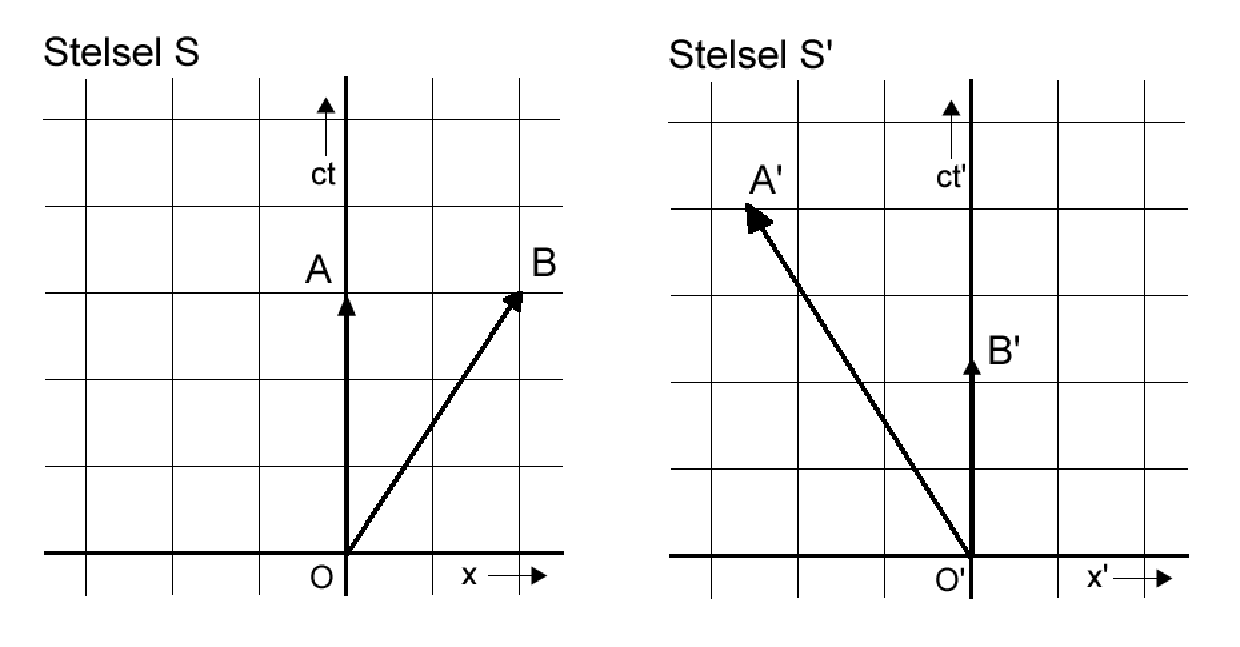
\epsfig{file=GridS1.pdf, width=0.8\textwidth}
\caption{{\sl \label{f:grid1} Wereldlijnen van waarnemer $A$ en $B$ uitgedrukt in stelsel $S$ en in stelsel $S'$.}}
\end{figure}

We kunnen nu de Lorentztransformaties gebruiken om de posities van $A$ en $B$ in het ruststelsel van de raket te bepalen (stelsel $S'$). De Lorentztransformaties geven:
\begin{eqnarray}\nonumber
A: \left(\begin{array}{c} ct \\ x \\ y \\ z \end{array}\right) &=&  
  \left(\begin{array}{c} 3 \\ 0 \\ 0 \\ 0 \end{array}\right) \mbox{lj} \\ \nonumber
A':  \left(\begin{array}{c} ct' \\ x' \\ y' \\ z' \end{array}\right) &=&  
  \left(\begin{array}{cccc} \gamma & -\beta \gamma & 0 & 0 \\ -\beta\gamma & \gamma & 0 & 0 \\ 0 & 0 & 1 & 0 \\ 0 & 0 & 0 & 1 \end{array}\right)
\left(\begin{array}{c} 3 \\ 0 \\ 0 \\ 0 \end{array}\right) =
\left(\begin{array}{c} 3\gamma \\ -2 \gamma \\ 0 \\ 0 \end{array}\right) \approx \left(\begin{array}{c} 4,02 \\ -2,68 \\ 0 \\ 0 \end{array}\right) 
 \mbox{lj}
\end{eqnarray}
en voor $B$ geeft dit (we laten nu de co\"ordinaten $y$ en $z$ weg)
\begin{eqnarray}\nonumber
B: \left(\begin{array}{c} ct \\ x \end{array}\right) &=&  
  \left(\begin{array}{c} 3 \\ 2 \end{array}\right) \mbox{lj} \\ \nonumber
B':  \left(\begin{array}{c} ct' \\ x' \end{array}\right) &=&  
  \left(\begin{array}{cc} \gamma & -\beta \gamma \\ -\beta\gamma & \gamma \end{array}\right)
\left(\begin{array}{c} 3 \\ 2 \end{array}\right) =
\gamma \left(\begin{array}{c} 5/3 \\ 0  \end{array}\right) \approx \left(\begin{array}{c} 2,23 \\ 0 \end{array}\right) 
 \mbox{lj}
\end{eqnarray}

De posities $A'$ en $B'$ zijn weergegeven in het
rechterfiguur~\ref{f:grid1}. Merk op dat in dit stelsel $A'$ en $B'$
niet meer gelijktijdig zijn.

\section{Causaliteit en de lichtsnelheid}
In het volgende verhaal willen we duidelijk maken dat de snelheid van
het licht de hoogste snelheid is waarmee informatie kan worden
overgedragen. We zullen dit laten zien aan hand van een tegenspraak:
als informatie sneller dan het licht zou kunnen worden overgedragen,
leidt dit tot verwarring van `oorzaak en gevolg'
(causaliteit). Causaliteit is een zeer fundamenteel principe in de
natuurkunde.  De `oorzaak' van een gebeurtenis vindt altijd plaats
voor het `gevolg'. Schending van causaliteit wordt nooit geaccepteerd
omdat dit leidt tot logische tegenspraak.  Het zou in principe immers
betekenen dat u uw voorouders kunt ombrengen voordat u geboren wordt.

Stel Anne en Frank zijn zijn vrienden. Frank gaat op ruimte reis met
een schip dat een snelheid van $\beta=0,6$ heeft (gebeurtenis $A$).  Na 4 jaar wachten
besluit Anne een brief aan Frank te sturen, met een nieuw type raket dat met
$\beta=3$ (!) kan reizen. Het moment van vertrek van deze raket noemen we $t=0$ en is gebeurtenis $B$.
Na 1 jaar in deze super-luminale raket is de brief bij Frank aangekomen (gebeurtenis $C$).

\begin{figure}[ht] 
\centering
%\includegraphics[width=.8\textwidth]{syllabus.pictures/GridS3}
\epsfig{file=GridS3.pdf, width=0.8\textwidth}
\caption{{\sl \label{f:grid3} Wereldlijnen van Anne ($A-B$), van Frank
($A-C$) en van de brief ($B-C$). Aan de linkerkant in het
co\"ordinatenstelsel in rust t.o.v. Anne, rechts in rust t.o.v. Frank. Frank
ziet de brief `uit de toekomst' komen.}}
\end{figure}


In het co\"ordinatenstelsel van Anne heeft Frank dus in 5 jaar een
totale afstand van 3 lj afgelegd, en ontvangt Frank de brief een jaar
nadat hij is verstuurd. Deze situatie is in weergegeven in het
linkerfiguur~\ref{f:grid3}. Maar in het stelsel in rust ten opzichte
van Frank, $S'$, is de situatie anders. Via de Lorentztransformaties
volgt:
\begin{eqnarray}\nonumber
A: \left( \begin{array}{c} ct \\ x \end{array} \right) = 
  \left( \begin{array}{c} -4 \\ 0 \end{array} \right) & \rightarrow & A': 
\left( \begin{array}{cc} \gamma & -\beta\gamma \\ -\beta\gamma & \gamma \end{array} \right)  
\left( \begin{array}{c} -4 \\ 0 \end{array} \right) = 
\left( \begin{array}{c} -5 \\ 3 \end{array} \right)  \\\nonumber
\end{eqnarray}
en evenzo voor $B'=(0,0)$ en $C'=(-1,3)$. In het co\"ordinatenstelsel
$S'$ bereikt Frank punt $C'$ eerder dan de brief die is verstuurd. Met
andere woorden, in zijn inertiaalsysteem komt de brief eerder aan dan
hij is verstuurd. Dit is in tegenspraak met causaliteit en daarmee
onmogelijk. Het is het gevolg van de aanname dat de brief met
$\beta=3$ werd verstuurd, en er kan geconcludeerd worden dat geen
informatie kan worden overgebracht met een snelheid groter dan $c$.

Merk op dat er overigens fenomenen in de natuur te vinden zijn die
wel sneller gaan dan de snelheid van het licht. Denk bijvoorbeeld aan
een lichtvlek die de lichtbundel van een vuurtoren maakt op een ver
weg gelegen eiland. Omdat de lichtbundel ronddraait zal de snelheid
waarmee de lichtvlek zich beweegt groter worden naarmate de afstand
tot de vuurtoren toeneemt. Er is geen limiet voor de snelheid van de
lichtvlek. Maar er wordt hierbij geen informatie overgedragen die
sneller gaat dan $c$!


\section{Minkowski-diagrammen}
In plaats van het tekenen van twee diagrammen voor de stelsels $S$ en
$S'$, kunnen beide stelsels ook in \'e\'en diagram getekend
worden. Dit wordt het Minkowski diagram genoemd.  Met deze ruimte-tijd
diagrammen kunnen de meeste vraagstukken van de speciale
relativiteitstheorie worden weergegeven, en deze geometrische
benadering is de meest elegante manier om de vraagstukken op te
lossen. Het is robuust omdat het inlevingsvermogen vraagt om de relatie
tussen gebeurtenissen en wereldlijnen te visualiseren.

 
Indien we het $(x,\ ct)$ vlak voorstellen m.b.v. twee loodrecht op
elkaar staande assen zoals in fig.~\ref{f:conseq2} dan wordt in deze
figuur de $x^{'}$-as beschreven door een lijn die volgt uit de eis
$ct^{'} = 0$, dus (zie formule \ref{v:lorentz11}.) $ct = \beta x$,
m.a.w. door een lijn met richtingsco\"{e}ffici\"{e}nt $\beta$.  Op
analoge wijze vinden we de lijn die de $ct^{'}$ as beschrijft uit de
eis $x^{'} = 0$, dus (zie formule \ref{v:lorentz10}.)  $x = \beta ct$,
of $ct = \frac{x}{\beta}$.  Dit is een lijn met
richtingsco\"{e}ffici\"{e}nt $\frac{1}{\beta}$.  D.w.z. de $x^{'}$-as
maakt met de $x$-as een hoek $\alpha$ z\'{o}, dat  $\tan \alpha = \beta$
en de $ct^{'}$-as maakt met de $ct$-as dezelfde hoek $\alpha$ zoals in
figuur \ref{f:conseq2} (Ga na.)\footnote{Op de website \url{www.nikhef.nl/\string~stanb/Minkowski.html} vindt u een flash animatie van het Minkowski-diagram.}.

% \begin{figure} [h]
% \begin{center}
% \mbox{\epsfxsize=8cm\epsffile{syllabus.pictures//minkowski.eps}}
% \caption{Minkowski diagram}
% \label{f:conseq2}
% \end{center}
% \end{figure}

\begin{figure}[ht]
\centering
%\includegraphics[width=.49\textwidth]{syllabus.pictures/minkowski}
\epsfig{file=minkowski.pdf, width=0.49\textwidth}
\caption{{\sl Minkowski-diagram}}
\label{f:conseq2}
\end{figure}


In figuur \ref{f:conseq2} is ook aangegeven de lijn $x = ct$:
de relatie tussen plaats en tijd voor een lichtstraal.
Deze lijn wordt ook wel als de lichtkegel aangeduid.
Twee `gebeurtenissen' $A$ en $B$ worden verbonden door een zogenaamde 
wereldlijn.
De lijn $AB$ in figuur \ref{f:conseq2} zou een eenparig bewegend deeltje kunnen voorstellen.
Verder is in de figuur aangegeven hoe het punt $(ct,x) = (1, 0)$ 
transformeert naar 
$(ct',x^{'}) = (\gamma,-\beta \gamma )$. 
(Ga na m.b.v. de Lorentztransformatie.)

%aanvulling september 2001
Het is gemakkelijk in te zien dat de eenheid van tijd (uitgedrukt in
$ct$) weergegeven t.o.v. systeem $S$ voor alle andere systemen $S'$
die t.o.v. $S$ eenparig langs de $x$-as bewegen op een hyperbool
liggen.  Immers: de grootheid $s^2=(ct)^2-x^2-y^2-z^2$ is een
invariant en deze vergelijking beschrijft een hyperbool in het
$(x,\ ct)$ vlak. We kunnen bijvoorbeeld nemen $(ct)^2-x^2=1$ en
verkrijgen zo de twee parabolen aangegeven in figuur~\ref{f:mink} (links) met
een `+'. Alle punten op deze parabool hebben dus dezelfde waarde voor
$s^2$. Een Lorentztransformatie van stelsel $S$ naar $S'$ is een
verschuiving langs deze parabolische baan.

Voor negatieve $s^2$ hebben we als karakteristieke hyperbool de
vergelijking $(ct)^{2}-x^2 = -1$, aangegeven in het figuur met een `-'
teken.

De lijnen voor $s^2=0$ zijn de wereldlijnen van die van het licht, en
komen overeen met de diagonale lijn van het figuur. Zij vormen de
`lichtkegel'. De lichtkegel is duidelijker als kegel te visualiseren
in de $(ct,x,y)$ ruimte, d.w.z., wanneer er twee ruimtelijke dimensies
getekend worden, zoals in figuur~\ref{f:mink} (rechts).

% \begin{figure} [h]
% \begin{center}
% \mbox{\epsfxsize=8cm\epsffile{syllabus.pictures//minkowski2.eps}}
% \caption{Hyperbolen in systeem $S$ waarop de co\"{o}rdinaten $ct' = 1$ 
% (hyperbolen aangegeven met '-') resp. $x' = 1$ (hyperbolen aangegeven
% met een '+') van alle mogelijke systemen $S'$ liggen.}
% \label{f:mink}
% \end{center}
% \end{figure}

\begin{figure}[ht]
\centering
%\includegraphics[width=.49\textwidth]{syllabus.pictures/minkowski2}
\epsfig{file=minkowski2.pdf, width=0.49\textwidth}
%\includegraphics[width=.49\textwidth]{syllabus.pictures/GridS5}
\epsfig{file=GridS5.pdf, width=0.49\textwidth}
\caption{{\sl Links: hyperbolen in systeem $S$ waarop de co\"{o}rdinaten $ct' = 1$ 
(hyperbolen aangegeven met '-') resp. $x' = 1$ (hyperbolen aangegeven
met een '+') van alle mogelijke systemen $S'$ liggen. Rechts: de lichtkegel voor co\"ordinaten $(ct,x,y)$.}}
\label{f:mink}
\end{figure}


Voor punten die `in' de lichtkegel liggen, dus in het gebied tussen de
asymptoten van de met `+' gelabelde hyperbolen, geldt dat er altijd
een Lorentztransformatie gevonden kan worden z\'{o} dat het punt in
het systeem $S'$ op de $ct'$-as ligt.  Viervectoren overeenkomend met
dergelijke punten noemen we tijdachtig (`timelike'). Gebeurtenissen in
elkaars lichtkegel volgen elkaar op, en er kan geen verwarring
ontstaan over welke gebeurtenis eerder of later plaatsvond. Wel kan het
onderlinge tijdsverschil veranderen indien het bekeken wordt vanuit een ander
stelsel, maar er is geen transformatie die de {\it volgorde} in de
tijd van de punten veranderd.  De gebeurtenissen zijn `causaal
verbonden', d.w.z. de gebeurtenis die eerder plaatsvond kan (mogelijkerwijs) invloed
hebben op een gebeurtenis die later plaatsvond: de informatie-overdracht van de eerste naar 
de tweede gebeurtenis kan slechts langzamer dan $c$ verlopen.



Viervectoren met co\"{o}rdinaten `buiten' de lichtkegel noemen we,
uiteraard, ruimteachtig (`spacelike'). Twee gebeurtenissen die een
onderlinge `ruimteachtige' afstand tot elkaar hebben kunnen elkaar op geen enkele manier
beïnvloeden en zijn hiermee dus niet causaal verbonden. De volgorde in
de tijd tussen deze gebeurtenissen hangt af van het stelsel waarin ze
beschreven worden. 


%einde aanvulling september 2001

Minkowski-diagrammen illustreren op heldere wijze allerlei
 kwalitatieve eigenschappen van de Lorentztransformatie, zoals de 
betrekkelijkheid van het begrip gelijktijdigheid (ga na) e.d.
In zekere zin zijn deze diagrammen echter ook verraderlijk, omdat de meetkunde 
van ruimte-tijd niet dezelfde is als de meetkunde van de ruimte alleen.
In het bijzonder is de grootte van een plaatsvector 
$\vec{r} = (x, y, z)$ gelijk aan $|\vec{r}| = \sqrt{x^{2} + y^{2} + z^{2}}$.
De grootte van de ruimte-tijd vector $r = (x, y, z, ct)$ is echter
$|r| = \sqrt{c^2 t^2 - x^{2} - y^{2} - z^{2}}$.
Deze grootte wordt dus berekend volgens een andere {\sl metriek}.
Om dit te ondervangen zette Minkowski zelf niet $ct$ maar $ict$ op de tijd-as
uit ($(ict)^{2} =  -c^{2}t^{2}$).
Dan is de standaard metriek te gebruiken. Deze truc is echter niet altijd vol
te houden.
We zullen de discussie hier niet verder voeren.

\subsection{Relativiteit van gelijktijdigheid}
We hadden eerder gezien dat gelijktijdigheid een relatief begrip is,
d.w.z., het hangt van het referentiestelsel van de waarnemer af of
twee gebeurtenissen gelijktijdig zijn of niet. We laten dat hier nogmaals
expliciet zien met gebruik making van ruimte-tijd diagrammen.

Hoe synchroniseren we twee klokken die op een afstand $l$ van elkaar
staan? Het meest eenvoudige is om een lamp in het midden te plaatsen,
het een lichtflits te laten uitzenden, en op het moment dat de
lichtflits aankomt beginnen de klokken te tikken. Het ruimte-tijd
diagram van deze situatie in het ruststelsel $S$ is getekend in
figuur~\ref{f:sync}, met de lamp in het midden en de twee klokken op
positie $\pm l/2$. De flits is gemarkeerd met F en het ontvangen van
de flits als G en H. Hierna beginnen de klokken te tikken zoals
aangegeven met stippen op de wereldlijn op de klok. Gelijktijdige
tikken liggen op de horizontale lijn die de tikken verbind, omdat zij
dezelfde tijd co\"ordinaat $ct$ hebben.

\begin{figure}[ht] 
\centering
%\includegraphics[width=.8\textwidth]{syllabus.pictures/Gelijktijdigheid}
\epsfig{file=Gelijktijdigheid.pdf, width=0.8\textwidth}
\caption{{\sl Het synchroniseren van twee klokken in stelsel $S$ dmv
het uitzenden van een lichtsignaal in het midden (F).  Elke klok
begint te tikken zodra de lichtflits is ontvangen (G en H). Lijnen van
gelijktijdigheid verbinden overeenkomstige tikken en zijn
horizontaal. \label{f:sync}}}
\end{figure}

Stel nu een ander referentiestelsel $S'$ voor, dat beweegt met een
snelheid $v=\beta c$ in de $x$-richting t.o.v. $S$.  In dit nieuwe
stelsel lopen de wereldlijnen van de klokken niet meer verticaal,
immers, zij verplaatsen met een snelheid $v$ als de tijd tikt. Volgens
het relativiteitsprincipe zullen de lichtsignalen nog steeds op lijnen
van 45$^o$ lopen. Het ruimte-tijd diagram in $S'$ ziet er dus uit
zoals in figuur~\ref{f:sync2}. Merk op dat de lijnen van
gelijktijdigheid scheef lopen in $S'$. Dit betekent dat twee
gebeurtenissen die simultaan zijn in $S$, in het algemeen niet meer
simultaan zijn in $S'$.

\begin{figure}[htb] 
\centering
%\includegraphics[width=.6\textwidth]{syllabus.pictures/Gelijktijdigheid2}
\epsfig{file=Gelijktijdigheid2.pdf, width=0.6\textwidth}
\caption{{\sl De klokken zoals geobserveerd in $S'$, samen met
gebeurtenissen F, G, H. Hoewel de klokken zijn gesynchroniseerd in
$S$, zijn ze dat niet in $S'$. Merk op dat de lijnen van
gelijktijdigheid scheef lopen in $S'$.\label{f:sync2} }}
\end{figure}

\subsection{De `ladder in de schuur'-paradox}
De boeren Niels (N) en Petra (P) hebben een schuur op het erf van
lengte $l$ en een ladder met lengte $2l$. Zij willen de ladder in de
schuur opbergen, maar deze is natuurlijk te lang. N stelt voor dat P
aankomt met de ladder met een snelheid $u=0,866c$. Bij deze snelheid
is $\gamma=2$ , en de ladder is met de Lorentzcontractie precies
genoeg korter geworden om in de schuur te passen. P heeft bezwaar. P
beargumenteerd dat als hij met de ladder aan het rennen is, in {\sl
zijn} co\"ordinatensysteem, de ladder nog steeds een lengte $2l$ heeft,
terwijl de schuur een Lorentzcontractie ondergaat en een lengte heeft
van $l/2$. Het plan om te gaan rennen met hoge snelheid heeft het
probleem alleen erger gemaakt.


Kunnen zij beide gelijk hebben? Stel voor dat P met de ladder
door de deur aan de voorkant van de schuur rent, en er via een andere
deur aan de achterkant weer uit komt. Stel verder voor dat de schuur
een mechaniek heeft waardoor de voordeur onmiddellijk sluit zodra de
achterkant van de ladder binnen is (noem dit gebeurtenis C), en een mechaniek waarmee de
achterdeur opent, precies op het moment wanneer de voorkant van de
ladder daar aangekomen is (gebeurtenis D). Er zijn nu twee
mogelijkheden: er is een tijd-interval waarin beide deuren gesloten
zijn of dit tijdsinterval is er
niet. Als dit tijdsinterval bestaat concluderen we dat de ladder past,
als het niet bestaat past de ladder niet. Wie heeft er gelijk?

\begin{figure}[ht] 
\centering
%\includegraphics[width=.8\textwidth]{syllabus.pictures/Schuurparadox}
\epsfig{file=Schuurparadox.pdf, width=0.8\textwidth}
\caption{{\sl Wereldlijnen van de voor- en achterkant van de schuur (G en H), en de voor en achterkant van de ladder (J en K) en gebeurtenissen 
C en D in het ruststelsel van N (figuur a) en in het ruststelsel van P (figuur b). Terwijl C en D gelijktijdig zijn in het stelsel van N,
zijn ze dit niet in het stelsel van P.\label{f:schuur}}}
\end{figure}


We kunnen ruimte-tijd plaatjes maken van de ladder en de schuur in
beide co\"ordinatenstelsels in rust voor N en P. In
figuur~\ref{f:schuur}, hebben de voor en achterkant van de schuur het
label G en H, en de voor en achterkant van de ladder label J en K. In
het co\"ordinatensysteem van N zijn inderdaad de gebeurtenissen C en D
gelijktijdig, dus is er een moment in de tijd van N dat de ladder in
de schuur past. In het stelsel van P echter, zijn deze gebeurtenissen
niet meer gelijktijdig! Gebeurtenis D vindt plaats v\`o\`ordat event C
plaatsvindt, dus is er geen tijd in het stelsel van P waarin de ladder
in zijn geheel in de schuur zit. Hiermee hebben beide waarnemers gelijk: de
vraag of de ladder in de schuur past is afhankelijk van het co\"ordinaten-stelsel;
het hangt af of twee gebeurtenissen gelijktijdig
zijn, en we hebben gezien dat gelijktijdigheid een relatief begrip is.
       % 26-03-2011 APC - polished plots									%+
% \include{SRT/Viervectoren}							%+
% \chapter{Klassieke Mechanica}
\vspace{-1cm}\begin{flushright}
{\it `If I have seen further than others, \\ it is by standing upon the shoulders of giants'}\\ I. Newton
\end{flushright}
Voordat we de effecten van de relativiteitstheorie op de mechanica
bespreken geven we een korte samenvatting van de Klassieke
Mechanica. Tijdens het college wordt gebruik gemaakt van het boek
`Analytical Mechanics' van \newline Fowles \& Cassiday (7de editie). 
\section{Dynamica}
De ontdekking van de wetten van de dynamica was een dramatisch moment
in de geschiedenis van de wetenschap. Voordat Newton zijn Principia
publiceerde waren de bewegingen van planeten een mysterie.
Galilei maakte daarvoor al een
grote stap met zijn principe van relativiteit; de grote bijdrage van Newton  was
dat hij beschreef hoe voorwerpen {\it veranderen} van snelheid.
Hij formuleerde daartoe drie hoofdwetten van de
Mechanica. De Eerste Wet was een herhaling van het relativiteitsprincipe van Galilei.
De Tweede Wet gaf specifiek aan hoe de snelheid van een voorwerp
verandert als een uitwendige {\it kracht} hierop inwerkt, via
$\vec{F}=m\vec{a}$. Newton geeft hierbij niet aan hoe de kracht in het
algemeen verkregen wordt; maar hij maakt ons bewust van het feit dat
er krachten zijn\footnote{In \'e\'en geval geeft hij wel een
uitdrukking voor de kracht, namelijk voor de zwaartekracht. Newton
geeft aan dat de gravitationele aantrekkingskracht tussen twee
lichamen met massa's $m$ en $M$ langs de verbinding van de
zwaartepunten van de twee lichamen loopt en gelijk is aan
\[ F_z = G \frac{mM}{r^2} \]
waarbij $r$ de onderlinge afstand tussen de lichamen is en $G$ de
Newtonse constante, $G=6,673 \cdot 10^{-11} m^3 kg^{-1} s^{-2}$. Voor
de aantrekking op aarde benaderen we dit als $F_z = m g $ waarbij de
valversnelling is, $g=G M/R^2$, met $R$ de diameter van de aarde. De
valversnelling op aarde is gelijk aan $g=9,8$ ms$^{-2}$. },
waarmee we de dynamica van voorwerpen kunnen beschrijven. Hoewel een
aantal verschijnselen hiermee beschreven kunnen worden, zoals de
draaiing van de maan om de aarde, zijn veel problemen hiermee niet
exact op te lossen. Bijvoorbeeld de onderlinge gravitationele aantrekking van drie
hemellichamen. Ook kende Newton lang niet alle krachten, zoals hij zich bijvoorbeeld 
zeker niet bewust was van de inter-moleculaire krachten.

Maar hoewel hij niet alle krachten kende, had hij wel een algemeen
principe waar alle krachten aan moeten voldoen. Dit principe is vastgelegd in zijn
Derde Wet: {\it actie is -reactie}.  Het wil ongeveer zeggen:
stel dat we twee voorwerpen hebben waarbij de eerste een kracht
uitoefent op het tweede, en het daarbij een kant op duwt. Dan
zegt de Derde Wet dat er een kracht is dat deeltje 2 uitoefent
op deeltje 1, die het de tegenovergestelde kant uitduwt. En dit
principe geldt voor alle krachten en voor een willekeurige
hoeveelheid deeltjes.
\subsection{Behoud van impuls}
De consequentie van de Derde Wet van Newton is het volgende. Stel dat we twee deeltjes beschouwen, $A$ en $B$, die botsen volgens Newton, waarbij deeltje A een kracht uitoefent op $B$ gelijk aan: 
\[ \vec{F}=m\vec{a} = \frac{d}{dt} m\vec{v} = \frac{d}{dt} \vec{p} \]
met $\vec{p}=m\vec{v}$ de impuls. De Derde Wet zegt nu dat er een
tegengestelde kracht van deeltje $B$ op $A$ wordt uitgeoefend, die
tegengesteld is:
\begin{equation}
\frac{dp_A}{dt} = -\frac{dp_B}{dt} \;\;\;\; \rightarrow \;\;\;\; \frac{d}{dt}(p_A+p_B) = 0
\end{equation}
waarbij we de impulsen $p_A$ en $p_B$ hebben opgeteld. Maar nu concluderen we
 dat de verandering van de {\it totale} impuls nul is, met andere woorden: de totale impuls $p_A+p_B$ is
behouden bij de interactie: het is een getal dat constant is als functie van de tijd.

We kunnen over het algemeen de wet van behoud van impuls voor een gesloten systeem, waarbij er geen interactie met de buitenwereld is, schrijven als
\begin{equation}
\vec{p}_1 + \vec{p}_2 +\vec{p}_3 + \vec{p}_4 + \dots = constant 
\end{equation} 
Indien er wel een uitwendige kracht op het systeem werkt, $\vec{F}_{ext}$, geldt dus
\begin{equation}
\frac{d}{dt}\left(\vec{p}_1 + \vec{p}_2 +\vec{p}_3 + \vec{p}_4 + \dots \right) = \vec{F}_{ext}
\end{equation}
\subsection{Arbeid en vermogen}
Als we de kracht als functie van de tijd $t$ kennen, kunnen we de fundamentele vergelijking $\vec{F}=\frac{d\vec{p}}{dt}$ voor de vergelijking van de dynamica van het deeltje oplossen door te integreren:
\begin{equation}
\int_A^B d \vec{p} = \int_{t_A}^{t_B} \vec{F} dt  \;\;\;\; \mbox{oftewel:} \;\;\;\;
\vec{p}_A-\vec{p}_B = \int_{t_A}^{t^B} \vec{F} dt = \vec{S}
\end{equation} 
waarbij $\vec{p}_A$ de impuls op moment $t_A$ is en $\vec{p}_B$ de
impuls op moment $t_B$. De grootheid $\vec{S}$ wordt de {\it krachtstoot}
genoemd. Dit wil zeggen dat de impulsverandering van het deeltje
gelijk is aan de krachtstoot.

Bij de meeste problemen in de mechanica is echter de kracht niet
gegeven als functie van de tijd $t$, maar als functie van de plaats,
$\vec{F}(x,y,z)$. We kunnen dan de integraal pas doen als we $x$, $y$
en $z$ als functies van de tijd kennen, d.w.z. als we het probleem
opgelost hebben dat we proberen op te lossen! Om uit deze vicieuze
cirkel te ontkomen voeren we de begrippen {\it arbeid} en {\it
energie} in.

Daartoe beschouwen we een bewegend deeltje dat een kracht
ondervindt. De hoeveelheid {\it arbeid} die door de kracht gedurende de
verplaatsing over een afstandje $d\vec{r}$ wordt verricht, is gelijk aan
\begin{equation}
dA = \vec{F} \cdot d \vec{r} 
\end{equation}
Rechts staat het inproduct, dus arbeid is gelijk aan het product van
de verplaatsing met de component van de kracht in de richting van de
verplaatsing. De arbeid is nul als de kracht loodrecht op de
verplaatsing staat. De totale arbeid wordt verkregen door de 
infinitesimale gedeelten bij elkaar op te tellen; dit levert de integraal:
\begin{equation}
A = \int_A^B \vec{F} \cdot d\vec{r} 
\end{equation}
In veel praktische gevallen is de kracht constant, zowel in grootte
als in de richting. We zullen ons nu daartoe beperken.  In dit geval
kunnen we de kracht $\vec{F}$ `buiten het integraalteken' halen (het
is immers een constante) en de arbeid schrijven als
\begin{equation}
A = \int_A^B \vec{F} \cdot d\vec{r} = \vec{F}\cdot \int_A^B d \vec{r} = \vec{F} \cdot(\vec{r}_B-\vec{t}_A) 
\end{equation}
Hieruit volgt dat de arbeid in dit geval onafhankelijk is van het pad
of de route tussen de punten $A$ en $B$. We kunnen willekeurig welke
route kiezen om van $A$ naar $B$ te gaan, bij een constante kracht is
de verrichtte arbeid onafhankelijk van de gekozen weg. Deze krachten
worden {\it conservatieve krachten} genoemd.

Bij praktische toepassingen is het van belang te weten in welk tempo arbeid verricht wordt. Het {\it vermogen} op een bepaald moment wordt gedefinieerd door 
\begin{equation}\label{e:vermogen}
P = \frac{dA}{dt}
\end{equation}
en dit kunnen we ook schrijven als
\begin{equation}\label{e:vermogen2}
P = F \cdot \frac{d \vec{r}}{dt} = \vec{F} \cdot \vec{v}
\end{equation}

We kunnen nu het verband bepalen tussen de arbeid en de energie. We
vullen hiervoor de uitdrukking $\vec{F} = m\vec{a}=md^2 \vec{r} /dt^2$ in voor de arbeid:
\begin{eqnarray}\label{e:arbeid}
A &=& \int_A^B \vec{F} \cdot d\vec{r} = \int_{t_A}^{t_B} \vec{F} \frac{d \vec{r}}{dt} dt =
\int_{t_A}^{t_B} m\frac{d^2\vec{r}}{dt^2} \frac{d \vec{r}}{dt} dt \\ \nonumber
& = &
\int_{t_A}^{t_B} \frac{d}{dt} \left[ \frac{1}{2} m\left( \frac{d r}{dt}\right)^2\right] dt =
\frac{1}{2} m\vec{v}_B^2 - \frac{1}{2}m\vec{v}_A^2
\end{eqnarray}
Deze uitkomst betekent dat de arbeid $A$ altijd gelijk is aan het verschil van de grootheid $\frac{1}{2}mv^2$
aan het einde en het begin van de baan. Dit wordt de kinetische energie genoemd, en aangeduid door $T$:
\begin{equation}
T=\frac{1}{2} m v^2 \;\;\;\; \mbox{of} \;\;\;\; T = \frac{p^2}{2m}
\end{equation}
De arbeid, verricht op een deeltje, is gelijk aan de verandering van
van kinetische energie van dit deeltje.

\subsection{Potenti\"ele energie}
We zagen dat een kracht conservatief heet als de arbeid die verricht
wordt onafhankelijk is van de afgelegde route. In dat geval kan de
arbeid worden uitgedrukt als het verschil tussen een grootheid
$U(x,y,z)$, berekend in het begin- en eindpunt. Deze grootheid
$U(x,y,z)$ wordt de potenti\"ele energie genoemd en is een functie van
de co\"ordinaten van een deeltje. Als $\vec{F}$ een conservatieve kracht
is geldt dus
\begin{equation}\label{e:pot}
A = \int_A^B \vec{F} \cdot d\vec{r} = U_A - U_B
\end{equation}
oftewel: de potenti\"ele energie is een functie zodanig dat de
verandering tussen begin- en eindpunt gelijk is aan de arbeid die op
het deeltje verricht moet worden om het van het begin- naar het
eindpunt te laten bewegen.
We hebben voor kleine afstanden $d\vec{r}$ dus voor de potenti\"ele energie
\begin{equation}
\vec{F} \cdot d\vec{r} = -d U 
\end{equation}
omdat we zo de definitie van de potenti\"ele energie weer terug vinden bij integratie:
\begin{equation}
A=\int_A^B \vec{F}\cdot d\vec{r} = -\int_A^B dU = -(U_B-U_A) = U_A-U_B
\end{equation}
We kunnen deze vergelijking schrijven als 
\begin{equation}
\vec{F} = -\vec{\nabla} U 
\end{equation}
waarbij de {\it gradi\"ent} $\vec{\nabla}$ de richtingsafgeleide is. De gradi\"ent is
zodanig gedefinieerd dat voor de $x$, $y$ en $z$ componenten van de kracht geldt dat:
\begin{equation}
F_x = -\frac{\partial U}{\partial x}, \;\;\;
F_y = -\frac{\partial U}{\partial y}, \;\;\;
F_z = -\frac{\partial U}{\partial z}
\end{equation} 
\subsection{Behoud van energie}
Als de kracht op een deeltje conservatief is, kunnen we vergelijking~\ref{e:pot}
combineren met~\ref{e:arbeid} en vinden dan dat $T_B-T_A = U_A-U_B$ oftewel:
\begin{equation}
(T+U)_A = (T+U)_B
\end{equation}
De grootheid $(T+U)$ wordt de {\it totale energie} van het deeltje genoemd en aangeduid met $W$, dus
\begin{equation}
W = T+U = \frac{1}{2} m v^2 + U(x,y,z)
\end{equation}
en er volgt dat als de krachten op een deeltje conservatief zijn, de
totale energie van dat deeltje behouden blijft, oftewel constant in de tijd is. De
totale energie wordt dus behouden. Voor een vrij vallend deeltje in een zwaartekrachtsveld bijvoorbeeld
geldt dat $U=mgh$ waarbij $h$ de hoogte van het deeltje is. Uit het
behoud van energie volgt
\begin{equation}
W = \frac{1}{2}m v^2 + mgh = constant
\end{equation}
Tot zover de zeer beknopte samenvatting van de Klassieke Mechanica.  

%
%\chapter{Relativistische mechanica}
%\section{Botsingen}
%We gaan nu terug naar de Speciale Relativiteitstheorie. We zullen allereerst een tweetal botsingen
%analyseren, waarbij we gebruik maken van de Lorentztransformaties. We zullen zien dat, indien we
%de behoudswetten willen handhaven samen met de Lorentztransformaties, we de definities van impuls 
%moeten aanpassen.
%\subsection{Elastische verstrooiing}
%We nemen allereerst aan dat de
%botsing 'perfect' is, dat wil zeggen dat geen energie verloren gaat
%in verwarming van de deeltjes en wrijving kan worden  verwaarloosd. Denk
%hierbij aan twee biljartballen op een perfect gladde biljarttafel. We
%noemen dit `elastische botsingen'. We nemen twee deeltjes die met
%snelheid $\vec{u}_1$ en $\vec{u}_2$ op elkaar afkomen en na de botsing
%een de snelheid $\vec{v}_1$ en $\vec{v}_2$ hebben. We schrijven het
%behoud van impuls op als:
%\begin{equation}
%\alpha_1\vec{u}_1 +\alpha_2 \vec{u}_2 = \alpha_3 \vec{v}_1 +\alpha_4 \vec{v}_2
%\end{equation} 
%waarbij in de Klassieke Mechanica we natuurlijk identificeren:
%\begin{eqnarray} 
%\alpha_1 & = & \alpha_3 \;\;\;\;\mbox{massa van deeltje 1} \\ 
%\alpha_2 & = & \alpha_4 \;\;\;\;\mbox{massa van deeltje 2} 
%\end{eqnarray}
%oftwel
%\[
%m_A\vec{u}_1 + m_B \vec{u}_2 = m_A\vec{v}_1' + m_B \vec{v}_2'  
%\]
%De massa $m$ noemen we de 'trage massa' van de deeltjes. In Figuur~\ref{f:bots} is deze botsing weergegeven. 
%\begin{figure}[ht] 
%\centering
%\includegraphics[width=.4\textwidth]{u1u2Horiz}
%\includegraphics[width=.2\textwidth]{u1u2Vert}
%\caption{{\sl Elastische botsing tussen twee identieke deeltjes die met gelijke snelheid op elkaar worden afgeschoten. In het rechterfiguur is de botsing `gedraaid' zodat deeltje 1 van onderaf komt en deeltje 2 van bovenaf.\label{f:bots}}}
%\end{figure}
%In de relativiteitstheorie zullen we een extra snelheidsafhankelijke
%term toevoegen in de definitie van impuls. 
%
%De elastische botsingen tussen twee identieke deeltjes die met
%dezelfde grootte van snelheid $|\vec{u}|$ op elkaar af worden
%geschoten heeft
%$|\vec{u}_1|=|\vec{u}_2|=|\vec{v}_1|=|\vec{v}_2|$. Bij deze botsing
%wordt wel de richting van de deeltjes veranderd, en de inkomende en
%uitgaande deeltjes maken een hoek $\theta$
%
%
%We gaan nu deze botsing beschouwen vanuit een co\"ordinatenstelsel dat
%meebeweegt met deeltje 1. In dit stelsel heeft deeltje 1 geen snelheid in de
%$x$-richting, maar alleeen een snelheid in de $y$-richting. We noemen dit snelheid $w$.
%Deeltje 2
%maakt een hoek $\alpha$ met de $x$-as. Deze situatie is getekend in Figuur~\ref{f:bots2}.
%We hebben nu de situatie dat:
%\begin{itemize}
%\item Deeltje 1 gaat nu 'recht omhoog' met snelheid $w_1$ en terug met 
%snelheid $w_2$. Deze snelheden zijn aan elkaar gelijk maar tegengesteld. 
%\item Deeltje 2 heeft in dit stelsel een grotere snelheid
%$\vec{V}$. De $x$-component van de snelheid is $u$ en de $y$-component noteren we als $v$.
%\end{itemize}
%\begin{figure}[ht] 
%\centering
%\includegraphics[width=.35\textwidth]{w1w2onder}
%\includegraphics[width=.35\textwidth]{w1w2boven}
%\caption{{\sl Links: Botsing tussen twee identieke deeltjes in het stelsel dat meebeweegt met deeltje 1.
%Rechts: Botsing tussen twee identieke deeltjes in het stelsel dat meebeweegt met deeltje 2.
%\label{f:bots2}}}
%\end{figure}
%
%
%We vragen ons nu af of we een relatie tussen de $y$-componenten van de
%impuls van deeltje 1 en 2 kunnen vinden, dus een relatie tussen $w$ en
%$v$. Kijk hiervoor naar een ander stelsel $S'$ dat met deeltje 2
%meebeweegt. In $S'$ heeft deeltje 2 dus geen $x$-component van de
%snelheid, maar deeltje 1 wel. Uit symmetrie-everwegingen volgt dat de
%situatie nu precies gelijk is aan die in stelsel $S$, met deeltjes 1
%en 2 omgewisseld. Maar voor de transformatie van de snelheden in de
%$y$-richting hadden we uitdrukking~\ref{e:vy}, oftewel
%\begin{equation}
%V_y = \frac{V_y'}{\gamma}\frac{1}{1-\frac{\beta}{c}V'_x}
%\end{equation}
% Verder volgt
%\begin{eqnarray}
%V'_y & = & w \\
%V'_x & = & 0
%\end{eqnarray}
%met andere woorden: we hebben gevonden dat $v=w/\gamma$ (let op, $w$
%is de $y$-component van de snelheid van deeltje 1 in $S$, en van
%deeltje 2 in $S'$; $v$ is de $y$-component van deeltje 2 in $S$ en deeltje 1 in $S'$).
%Merk nu op dat:
%\begin{enumerate}
%\item De totale snelheid van bewegend deeltje 1 in $S$ en van bewegend deeltje 2 in $S'$ is hetzelfde, namelijk: $V=\sqrt{v^2+u^2}$.
%\item Impulsbehoud in de $y$-richting geeft nu
%\begin{equation}
%\alpha(w) w - \alpha(V) v = -\alpha(w) w + \alpha(V) v
%\end{equation}
%en let hierbij goed op het verschil tussen $V$ en $v$ en de tekens! We hebben nu
%\begin{equation}
%\frac{\alpha(V)}{\alpha(w)} = \frac{w}{v} = \frac{w}{w/\gamma} = \gamma \label{e:imprat}
%\end{equation}
%\end{enumerate}
%Neem nu de snelheid $w$ heel klein. In deze limiet is
%$\lim_{w\rightarrow 0} v = 0$ en $\lim_{w\rightarrow 0} V = u$. In dat
%geval kunnen we de relativistische effecten verwaarlozen en moeten we
%de Klassieke uitdrukking voor impuls terugvinden. Dit houdt in dat 
%\begin{equation}
%\lim_{w\rightarrow 0} \alpha(w) = m 
%\end{equation}
%en hiermee (invullen in~\ref{e:imprat}) vinden we
%\begin{equation}
%\lim_{w\rightarrow 0} \alpha(V) = \gamma m = \frac{m}{\sqrt{1-\frac{u^2}{c^2}}}
%\end{equation}
%We moeten dus de definitie van impuls aanpassen om te zorgen dat deze behouden blijft. Deze relativistische
%uitbreiding van impuls is
%\begin{equation}\label{e:impuls}
%\vec{p} = \gamma m \vec{v}
%\end{equation}
%Met deze definitie kunnen we de elastische botsingen relativistisch beschrijven. De factor $\gamma$ 
%is toegevoegd als gevolg van de transformatie van de snelheid in de $y$ richting.
%\subsection{Inelastische verstrooiing}
%We zullen nu een heel ander type botsingen beschouwen, namelijk de inelastische botsing. Hierbij 
%botsen twee deeltjes op elkaar zonder dat ze terugstoten. Denk nu aan twee klompen klei die
%op elkaar worden geschoten en na de botsing een grote klomp vormen. 
%
%\begin{figure}[ht] 
%\centering
%\includegraphics[width=.9\textwidth]{2mtotM}
%\caption{{\sl Links: Inelastische botsing tussen twee identieke deeltjes. Links in het stelsel waarin
%deeltje $M$ in rust is, rechts in het stelsel waarin $M$ een kleine snelheid $\vec{u}$ heeft. 
%Rechts: Botsing tussen twee identieke deeltjes in het stelsel dat meebeweegt met deeltje 2.
%\label{f:bots3}}}
%\end{figure}
%
%
%Neem twee identieke deeltjes met massa $m$ die een inelastische botsing maken. Beide komen met snelheid $w$ naar elkaar toe. Na de botsing is er \'e\'en stilstaand deeltje over met massa $M$. Klassiek verwachten
%we dat geldt $M=2m$.
%
%We beschouwen nu dezelfde botsing vanuit een stelsel dat met een kleine snelheid $u$ in de $y$-richting beweegt. De impuls voor en na de bosting in de $y$ richting levert:
%\begin{eqnarray}
%\mbox{voor} & p = & 2 \gamma m u \\
%\mbox{na}   & p = & M u 
%\end{eqnarray}
%waarbij we de relativistische definitie van de impuls hebben gebruikt, zie vergelijking~\ref{e:impuls}. We nemen weer de limiet $u\rightarrow 0$ en factor $\gamma$ staat dan voor $\gamma = 1/\sqrt{1-w^2/c^2}$.
%We hebben nu dus gevonden dat geldt:
%\begin{equation}
%M = 2\gamma m = \frac{2m}{\sqrt{1-\frac{w^2}{c^2}}}
%\end{equation}
%en dus is de massa $M$ na de botsing {\it groter} dan de som van de
%twee (rust-) massa's voor de botsing!  Dit is ook het gevolg van de
%wet van behoud van impuls. We zullen zien dat de toename van massa na
%de botsing afkomstig is van de kinetische energie v\`o\`or de botsing.
%\section{Relativistische energie}
%We geven eerst het gedachte experiment van Einstein waarin de
%gelijkheid van energie en massa werd gepostuleerd.  Dit
%gedachte-experiment is ook gepubliceerd in 1905, en is te vinden in de
%reader bij dit college. Vervolgens zullen we de energie van een bewegend voorwerp 
%beschouwen. 
%\subsection{De doos van Einstein}
%Als er \'e\'en natuurkundige wet is die iedereen kent, is dat wel de beroemde wet van equivalentie 
%tussen massa en energie
%\begin{equation}
%E= m c^2
%\end{equation}
%Einstein toonde deze wet eerst aan met een eenvoudig
%gedachteexperiment. In 1905 had hij eerst een verklaring voor het
%foto-elektrisch effect gegeven. Dit beschrijft het fenomeen waarbij
%licht op een plaatje valt en elektronen losmaakt. De energie van de
%elektronen bleek af te hangen van de `kleur' van het licht, en niet
%van de intensiteit van de lichtbron. De verklaring werd door Einstein
%gegeven door licht voor te stellen als deeltjes, fotonen, elk met een
%energie $E_{\gamma} = h \nu$. De constante $h$ is de constante van
%Planck en heeft de waarde $h=6.626\cdot 10^{-34} $kg m$^2$ s$^{-1}$, en
%$\nu$ staat voor de frequentie van het licht. De impuls van een foton
%is omgekeerd evenredig met de golflengte $\lambda$ en wordt gegeven
%door $p_{\gamma}=h/\lambda$. Met de uitdrukking $\lambda \nu = c$ is
%hiermee gegeven dat
%\[
%E_{\gamma} = c p_{\gamma}
%\]
%
%Het gedachte-experiment van Einstein (`Einsteins doos') gaat nu als
%volgt. Stel je een doos voor, volledig afgesloten van de
%buitenwereld. De doos heeft een massa $M$. Aan de linkerkant van de
%doos wordt nu een foton uitgestraald door de wand, en vertrekt naar de
%rechterkant van de doos. Op het moment van vertrek krijgt de doos een
%terugstoot van het vertrekkend foton. De impuls van het foton
%wordt gegeven door $p_{\gamma}=E/c$ en de impuls van de terugstoot
%door $p=Mv$. Met andere woorden, de snelheid van de doos, $v$, door de terugstoot is gelijk aan
%$v=-p/M = -E/ cM$. We hebben hier de klassieke benadering voor de impuls genomen.
%
%
%Op het moment dat het foton aan de andere kant aankomt wordt de
%terugstoot tenietgedaan en staat de doos weer stil. De doos is dan
%verplaatst over een afstand $\Delta x$. Deze afstand is gelijk aan $\Delta x=v \Delta t$,
%waarbij $\Delta t$ de tijd voorstelt die het foton er over doet om door de
%doos te vliegen, $\Delta t = L/c$ met $L$ de grootte van de doos.
%Hiermee is dus de afgelegde afstand $\Delta x=-vL/c = -EL/c^2 M$. 
%
%\begin{figure}[ht] 
%\centering
%\includegraphics[width=.5\textwidth]{EinsteinBox}
%\caption{{\sl De `doos van Einstein'. Voor de uitleg zie tekst.
%\label{f:bots4}}}
%\end{figure}
%
%
%Het foton heeft pure energie getransporteerd; geen massa! Maar het
%zwaartepunt van de doos, dat geen kontakt met de buitenwereld heeft, kan door deze
%aktie van het foton niet verplaatst zijn. Als er een massa $m$ verplaatst zou zijn geweest, 
%over de lengte $L$ van de doos, zegt het behoud van het zwaartepunt:
%\[
%mL + M\Delta x = 0
%\]
%Nu kunnen we invullen voor $\Delta x$ en krijgen:
%\[
% mL - M\frac{EL}{c^2M} = 0\;\;\;\; \mbox{oftewel:} \;\;\;\; L\left(m-\frac{E}{c^2}\right) = 0
%\]
%en hiermee $E=mc^2$!
%
%Met andere woorden: de pure energie $E$ van het foton is equivalent aan een massa $m$ waarvoor geldt
%$m=E/c^2$. Het is aan Einstein te danken dat hij deze relatie algemeen heeft opgevat: energie is 
%gelijk aam massa.
%
%\subsection{Energie van een bewegend voorwerp}
%Met het gedachteexperiment heeft Einstein aangetoond dat energie en
%massa aan elkaar gelijk zijn via de relatie $E=mc^2$. Voor een
%voorwerp dat met een snelheid beweegt hebben we aangetoond dat de
%impuls wordt aangepast, en de relativistische beschrijving wordt
%gegeven door
%\begin{equation}\label{e:impulsmov}
%\vec{p} = \gamma m \vec{v}
%\end{equation} 
%Zo kunnen we ook postuleren dat de energie van het voorwerp gelijk is aan
%\begin{equation}\label{e:energymov}
%E = \gamma m c^2
%\end{equation} 
%en we zullen aantonen dat we met deze uitdrukking de juiste Klassieke Limiet verkregen wordt. 
%Immers, we kunnen voor lage snelheden benaderen dat
%\[
%\gamma  = \frac{1}{\sqrt{1-\frac{v^2}{c^2}}} \sim \left( 1 + \frac{v^2}{2c^2} - 
%\frac{3}{8}\frac{v^4}{c^4}\right)  
%\]
%en vinden dus dat
%\[
%E = \gamma m c^2 ~ mc^2 + \frac{1}{2} m v^2 - \frac{3}{8} m v^4 / c^2
%\]
%In de limiet voor lage snelheden is dit is precies de kinematische energie $\frac{1}{2}mv^2$ 
%plus een constante, $mc^2$. Energiebehoud wordt door dergelijke 
%constanten uiteraard netjes intact gelaten.
%
%We zullen nu ook laten zien dat deze definitie voor de energie,
%vergelijking~\ref{e:energymov}, overeenstemt met de klassieke relatie
%tussen energie en kracht, zoals gegeven in
%vergelijkingen~\ref{e:vermogen} en~\ref{e:vermogen2}. We hebben gezien dat verandering van energie
%$dE/dt$ teweeg wordt gebracht door het vermogen $\vec{F}\cdot \vec{v}$. Invullen levert:
%\begin{equation}
%\frac{dE}{dt} = \frac{d\gamma m c^2 }{dt} = \vec{v}\cdot \vec{F} = \vec{v} \cdot \frac{d\vec{p}}{dt}  = \vec{v}\frac{d\gamma m\vec{v}}{dt}
%\end{equation}
%We zullen nu laten zien dat deze vergelijking inderdaad consistent is. Daartoe vermenigvuldigen we met $2\gamma m$ om tot totale afgeleiden te komen:
%\begin{eqnarray}
%2\gamma m c^2 \frac{d\gamma m}{dt} = 2\gamma m \vec{v} \cdot \frac{d\gamma m \vec{v}}{dt} \\
%c^2 \frac{d}{dt} \left( \gamma m\right)^2 = \frac{d}{dt}\left( \gamma m v\right)^2
%\end{eqnarray}
%Hieruit volgt dat moet gelden:
%\[
%c^2 \gamma^2 m^2 = \gamma^2 m^2 v^2 +C
%\]
%waarbij $C$ een integratieconstante is, en het inproduct $\vec{v}\cdot \vec{v}$ geschreven wordt als $v^2$. Om de integratieconstante te bepalen vullen we snelheid $v=0$ in. Dan is $\gamma=1$ en volgt:
%\[
%c^2 m^2 = C
%\]
%zodat we kunnen schrijven
%\[
%c^2\gamma^2 m^2 - \gamma^2 m^2 v^2 = c^2 m^2
%\]
%waaruit we kunnen afleiden dan moet gelden dat 
%\[
%\gamma^2 = \frac{c^2}{c^2-v^2} = \frac{1}{1-\frac{v^2}{c^2}}
%\]
%hetgeen precies is wat we verwachten voor $\gamma$. Met andere woorden: de relativistische 
%uitdrukking voor de energie stemt overeen met de relaties tussen energie en kracht zoals gegeven door de Klassieke Mechanica.
%
%
%
%
%\section{Energie-impuls vector}
%We kunnen de relativistische uitdrukkingen voor energie en impuls ook
%op een ander manier benaderen. Daartoe keren we terug naar de
%vier-vectoren $x=(ct,x,y,z)$, en vragen ons af of er nog andere
%vier-vectoren te defini\"eren zijn.
%
%Daartoe laten we ons inspireren door de definitie van impuls in de Klassieke Mechanica: 
%\[
%\vec{p} = m\vec{v} = \lim_{\Delta t \rightarrow 0} m\frac{\Delta \vec{x}}{\Delta t}
%\]
%waarbij $\Delta x$ de verplaatsing in de $x$-richting is en $\Delta t$
%de tijdsduur. We vragen ons af of hier een equivalente vier-vector van
%te maken is in de vier-dimensionale ruimte-tijd. Dit is inderdaad
%mogelijk door $\Delta \vec{x}$ te vervangen door de viervector $\Delta x$.
%We kunnen echter niet $\Delta t$ in de noemer laten staan, omdat deze niet invariant onder de Lorentz
%transformaties is. We kunnen wel $\Delta t$ vervangen door het verloop van de eigentijd, $\Delta \tau$,
%omdat $\tau$ immers een scalar is. Als vier-vector kunnen we dus schrijven:
%\begin{equation}
%p =(p_0,p_1,p_2,p_3) =  \left( m\frac{c\Delta t}{\Delta \tau}, m \frac{\Delta x}{\Delta \tau}
%, m \frac{\Delta y}{\Delta \tau}, m \frac{\Delta z}{\Delta \tau}\right)
%\end{equation}
%en de vier-vector $p$ van  een voorwerp heeft nu de richting langs de wereldlijn van dit
%voorwerp in de ruimte-tijd. Voor de limiet $\Delta \tau\rightarrow 0$ kunnen we de componenten
%van de vier-vector identificeren als:
%\begin{eqnarray}
%p_0 & = & \frac{E}{c} \\
%p_1 & = & p_x \\
%p_2 & = & p_y \\
%p_3 & = & p_z 
%\end{eqnarray}
%immers, voor de componenten geldt:
%\begin{eqnarray}
%\frac{E}{c} & = & m c \frac{dt}{d\tau} = \gamma m c\\
%p_x & = & m \frac{dx}{d\tau} = \gamma mv_x \\
%p_y & = & m \frac{dy}{d\tau} = \gamma mv_y \\
%p_z & = & m \frac{dz}{d\tau} = \gamma mv_z 
%\end{eqnarray}
%Alle vier deze componenten zijn behouden bij een interaktie (d.w.z.
%botsing). De componenten zijn niet hetzelfde in elk stelsel $S$ of
%$S'$. Wel is de lengte van de vier-vector invariant, met andere
%woorden, de uitdrukking
%\begin{equation}
%\left(\frac{E}{c}\right)^2 - |\vec{p}|^2 
%\end{equation}
%is hetzelfde in elk stelsel. Deze uitdrukking is gelijk aan:
%\begin{eqnarray}\nonumber
%|p|^2 & = &  \left(\frac{E}{c}\right)^2 - |\vec{p}|^2  \\
%      & = & m^2c^2 \frac{dt^2}{d\tau^2}-m^2\frac{dx^2}{d\tau^2}-m^2\frac{dy^2}{d\tau^2}-m^2\frac{dz^2}{d\tau^2}\\ \nonumber
%      & = & m^2\frac{\left(d c^2 t^2 - dx^2 - dy^2 - dz^2\right)}{d\tau^2} \\ \nonumber
%      & = & m^2 c^2 \frac{d\tau^2}{d\tau^2} \\ \nonumber
%      & = & m^2 c^2
%\end{eqnarray}
%we kunnen dit schrijven als
%\begin{equation}
%E^2 - c^2 |\vec{p}|^2 = m^2 c^4
%\end{equation}
%en dit is de relativistische relatie tussen energie en impuls. Het is
%niets anders dan de lengte van de vier-vector $p$. Het `min'-teken is
%deze uitdrukking is hetzelfde `min'-teken als we al eerder zagen in de
%Minkowski-ruimte: dit maakte de ruimte-tijd fundamenteel anders dan de
%Euclidische ruimte.
%
%Merk verder op dat $m$ een invariante grootheid is, die hetzelfde is in alle stelsels. De uidrukking is
%overigens {\it kwadratisch} voor de energie, dus heeft de energie zelf twee oplossingen, namelijk $E=\pm 
%\sqrt{m^2 c^4 + c^2 |\vec{p}|^2}$. Dit zal uiteindelijk, wanneer het gecombineerd wordt met de quantummechanica, aanleiding geven tot het bestaan van anti-materie.
%
%De Lorentz-transformatie voor de componenten van de vier-vector $p$ kunnen verkregen worden door de componenten in te vullen. Het levert op voor een boost langs de $x$-as:
%\begin{eqnarray}
%\frac{E'}{c} &=& \gamma\left(\frac{E}{c} - \beta p_x \right) \\
%p_x' & = & \gamma\left( p_x - \beta \frac{e}{c}\right) \\
%p_y' & = & p_y \\
%p_z' & = & p_z
%\end{eqnarray}
%
%
%\subsection{Massaloze deeltjes}
%We zien dat de relativiteitstheorie massaloze deeltjes toelaat:
%\begin{displaymath}
%E = pc
%\end{displaymath}
%leidt tot
%\begin{displaymath}
%M = 0
%\end{displaymath}
%Aangezien uit formules \ref{e:impulsmov} en \ref{e:energymov} volgt dat
%\begin{displaymath}
%p = \frac{E}{c} \beta 
%\end{displaymath}
%(ga na) geldt voor massaloze deeltjes dus:
%\begin{displaymath}
%p = \frac{pc}{c} \beta = p \beta
%\end{displaymath}
%Hieruit volgt dat $\beta = 1$, dus $v = c$.
%M.a.w. massaloze deeltjes bewegen met de lichtsnelheid; zij kunnen niet stilstaan. Het foton
%is het bekendste voorbeeld. 
%
%\section{Samenvatting}
%De relativistische relatie tussen energie, impuls en snelheid kan worden samengevat als:
%\begin{eqnarray}
%E\leftrightarrow \vec{p} & \mbox{:} & E^2 - c^2 |\vec{p}|^2 = m^2 c^4 \\ \nonumber
%E\leftrightarrow \vec{v} & \mbox{:} & E = \gamma m c^2 \\ \nonumber
%\vec{p} \leftrightarrow \vec{v} & \mbox{:} & \vec{p} = \gamma m \vec{v} 
%\end{eqnarray}
%De relatie tussen de energie, impuls en snelheid wordt gegeven door:
%\begin{equation}
%\frac{c\vec{p}}{E} = \frac{\gamma m \vec{v} c}{\gamma m c^2} = \frac{\vec{v}}{c} = \vec{\beta}
%\end{equation}
%dus 
%\begin{equation}
%\vec{\beta} = \frac{\vec{v}}{c} = \frac{c\vec{p}}{E}
%\end{equation}
%
%\section{Enige opmerkingen n.a.v. botsingen} 
%
%In de beschrijving van een botsing tussen een willekeurig aantal
%deeltjes kunnen we nog het volgende opmerken. Bij de botsing
%zijn de {\it ingaande} deeltjes te onderscheiden van de {\it
%uitgaande} deeltjes. Voor een systeem van $n$ ingaande deeltjes en
%$m$ uitgaande deeltjes gelden de volgende behoudswetten:
%\begin{eqnarray}
%\sum_{deeltjes}^n p_x^{in} & = & \sum_{deeltjes}^m p_x^{uit} \\ \nonumber
%\sum_{deeltjes}^n p_y^{in} & = & \sum_{deeltjes}^m p_y^{uit} \\ \nonumber
%\sum_{deeltjes}^n p_z^{in} & = & \sum_{deeltjes}^m p_z^{uit} \\ \nonumber
%\sum_{deeltjes}^n E^{in} & = & \sum_{deeltjes}^m E^{uit}
%\end{eqnarray}
%Dit zijn de behoudswetten van de botsing: dat wil zeggen dat deze grootheden, impuls en energie, 
%voor en na de botsing hetzelfde zijn. Deze grootheden hangen af van het stelsel $S$ waarin we de botsing 
%beschouwen. De invariant $E^2-c^2|\vec{p}|^2$ is hetzelfde in elk co\"ordinatenstelsel $S$. Deze grootheid is ook behouden voor het hele systeem, maar niet voor elk deeltje afzonderlijk.
%
%De `massa van een systeem' leidt soms tot verwarring. Een lichaam met grote temperatuur heeft meer energie en 
%dus een grotere massa. Bijvoorbeeld, water van 40$^o$ C heeft een grotere massa dan water van 15$^o$ C. De toename in massa is ongeveer een fractie 10$^{-12}$. Maar wat neemt er nu eigenlijk toe? Niet de massa van de individuele
%molekulen. Het is de (bewegings) energie van het systeem van molekulen dat toeneemt.
%
%Neem als voorbeeld 2 voorwerpen met beide een massa van 8 kg. Dit is de massa als de voorwerpen in rust zijn.
%Schiet de voorwerpen nu uit elkaar, in tegenovergestelde richting, elk met een impuls van 6$c$ kg.
%De energie van elk voorwerp is nu
%\[
%E=\sqrt{m^2c^4+p^2c^2} = \sqrt{8^2 c^4 + 6^2 c^4} = 10 c^2 \mbox{kg}
%\]
%Voor dit systeem is de totale impuls en energie gelijk aan
%\[
%p_{tot} = 6c-6c = 0 \;\;\;\; ; \;\;\;\; E_{tot} = 10 c^2 + 10 c^2 = 20c^2 \mbox{kg}
%\]
%De massa van het systeem wordt hiermee gelijk aan
%\[
%M_{tot} = \sqrt{E^2/c^4 - p^2/c^2} = \sqrt{ 20^2 - o^2 } = 20  \mbox{kg}
%\]
%We zien dat de totale massa van het systeem, 20 kg, niet overeenkomt met de som van de massa's van de individuele
%voorwerpen, 2 maal 6 kg. De toename van de massa van het systeem komt overeen met de toename van de energie van het systeem.
%
%
% 
                 % eerste deel H6
\chapter{Relativistische mechanica}

\section{Botsingen}
We gaan nu terug naar de Speciale Relativiteitstheorie. We zullen allereerst een tweetal botsingen
analyseren, waarbij we gebruik maken van de Lorentztransformaties. We zullen zien dat, indien we
de behoudswetten willen handhaven samen met de Lorentztransformaties, we de definities van impuls 
moeten aanpassen.
\subsection{Elastische verstrooiing}
We nemen allereerst aan dat de
botsing `perfect' is, dat wil zeggen dat geen energie verloren gaat
in verwarming van de deeltjes en wrijving kan worden  verwaarloosd. Denk
hierbij aan twee biljartballen op een perfect gladde biljarttafel. We
noemen dit `elastische botsingen'. We nemen twee deeltjes die met
snelheid $\vec{u}_1$ en $\vec{u}_2$ op elkaar afkomen en na de botsing
een snelheid $\vec{v}_1$ en $\vec{v}_2$ hebben. We schrijven het
behoud van impuls op als:
\begin{equation}
\alpha_1\vec{u}_1 +\alpha_2 \vec{u}_2 = \alpha_3 \vec{v}_1 +\alpha_4 \vec{v}_2
\end{equation} 
waarbij in de Klassieke Mechanica we natuurlijk identificeren:
\begin{eqnarray} 
\alpha_1 & = & \alpha_3 \;\;\;\;\mbox{massa van deeltje 1} \\ 
\alpha_2 & = & \alpha_4 \;\;\;\;\mbox{massa van deeltje 2} 
\end{eqnarray}
oftewel
\[
m_A\vec{u}_1 + m_B \vec{u}_2 = m_A\vec{v}_1' + m_B \vec{v}_2'  
\]
De massa $m$ noemen we de `trage massa' van de deeltjes. In Figuur~\ref{f:bots} is deze botsing weergegeven. 
\begin{figure}[ht] 
\centering
\epsfig{file=u1u2Horiz.pdf, width=0.4\textwidth}
\epsfig{file=u1u2Vert.pdf, width=0.2\textwidth}
\caption{{\sl Elastische botsing tussen twee identieke deeltjes die met gelijke snelheid op elkaar worden afgeschoten. In het rechterfiguur is de botsing `gedraaid' zodat deeltje 1 van onderaf komt en deeltje 2 van bovenaf.\label{f:bots}}}
\end{figure}
In de relativiteitstheorie zullen we een extra snelheidsafhankelijke
term toevoegen in de definitie van impuls. 

De elastische botsingen tussen twee identieke deeltjes die met
dezelfde grootte van snelheid $|\vec{u}|$ op elkaar af worden
geschoten heeft
$|\vec{u}_1|=|\vec{u}_2|=|\vec{v}_1|=|\vec{v}_2|$. Bij deze botsing
wordt wel de richting van de deeltjes veranderd, en de inkomende en
uitgaande deeltjes maken een hoek $\theta$.


We gaan nu deze botsing beschouwen vanuit een co\"ordinatenstelsel dat
meebeweegt met deeltje 1. In dit stelsel heeft deeltje 1 geen snelheid in de
$x$-richting, maar alleen een snelheid in de $y$-richting. We noemen dit snelheid $w$.
Deeltje 2
maakt een hoek $\alpha$ met de $x$-as. Deze situatie is getekend in Figuur~\ref{f:bots2}.
We hebben nu de situatie dat:
\begin{itemize}
\item Deeltje 1 gaat nu `recht omhoog' met snelheid $w_1$ en terug met 
snelheid $w_2$. Deze snelheden zijn aan elkaar gelijk maar tegengesteld. 
\item Deeltje 2 heeft in dit stelsel een grotere snelheid
$\vec{V}$. De $x$-component van de snelheid is $u$ en de $y$-component noteren we als $v$.
\end{itemize}
\begin{figure}[ht] 
\centering
%\includegraphics[width=.35\textwidth]{syllabus.pictures/w1w2onder}
%\includegraphics[width=.35\textwidth]{syllabus.pictures/w1w2boven}
\epsfig{file=w1w2onder.pdf, width=0.35\textwidth}
\epsfig{file=w1w2boven.pdf, width=0.35\textwidth}
\caption{{\sl Links: Botsing tussen twee identieke deeltjes in het stelsel dat meebeweegt met deeltje 1.
Rechts: Botsing tussen twee identieke deeltjes in het stelsel dat meebeweegt met deeltje 2.
\label{f:bots2}}}
\end{figure}


We vragen ons nu af of we een relatie tussen de $y$-componenten van de
impuls van deeltje 1 en 2 kunnen vinden, dus een relatie tussen $w$ en
$v$. Kijk hiervoor naar een ander stelsel $S'$ dat met deeltje 2
meebeweegt. In $S'$ heeft deeltje 2 dus geen $x$-component van de
snelheid, maar deeltje 1 wel. Uit symmetrie-overwegingen volgt dat de
situatie nu precies gelijk is aan die in stelsel $S$, met deeltjes 1
en 2 omgewisseld. Maar voor de transformatie van de snelheden in de
$y$-richting hadden we uitdrukking~\ref{e:vy}, oftewel
\begin{equation}
V_y = \frac{V_y'}{\gamma}\frac{1}{1-\frac{\beta}{c}V'_x}
\end{equation}
 Verder volgt
\begin{eqnarray}
V'_y & = & w \\
V'_x & = & 0
\end{eqnarray}
met andere woorden: we hebben gevonden dat $v=w/\gamma$ (let op, $w$
is de $y$-component van de snelheid van deeltje 1 in $S$, en van
deeltje 2 in $S'$; $v$ is de $y$-component van deeltje 2 in $S$ en deeltje 1 in $S'$).
Merk nu op dat:
\begin{enumerate}
\item De totale snelheid van bewegend deeltje 1 in $S$ en van bewegend deeltje 2 in $S'$ is hetzelfde, namelijk: $V=\sqrt{v^2+u^2}$.
\item Impulsbehoud in de $y$-richting geeft nu
\begin{equation}
\alpha(w) w - \alpha(V) v = -\alpha(w) w + \alpha(V) v
\end{equation}
en let hierbij goed op het verschil tussen $V$ en $v$ en de tekens! We hebben nu
\begin{equation}
\frac{\alpha(V)}{\alpha(w)} = \frac{w}{v} = \frac{w}{w/\gamma} = \gamma \label{e:imprat}
\end{equation}
\end{enumerate}
Neem nu de snelheid $w$ heel klein. In deze limiet is
$\lim_{w\rightarrow 0} v = 0$ en $\lim_{w\rightarrow 0} V = u$. In dat
geval kunnen we de relativistische effecten verwaarlozen en moeten we
de Klassieke uitdrukking voor impuls terugvinden. Dit houdt in dat 
\begin{equation}
\lim_{w\rightarrow 0} \alpha(w) = m 
\end{equation}
en hiermee (invullen in~\ref{e:imprat}) vinden we
\begin{equation}
\lim_{w\rightarrow 0} \alpha(V) = \gamma m = \frac{m}{\sqrt{1-\frac{u^2}{c^2}}}
\end{equation}
We moeten dus de definitie van impuls aanpassen om te zorgen dat deze behouden blijft. Deze relativistische
uitbreiding van impuls is
\begin{equation}\label{e:impuls}
\vec{p} = \gamma m \vec{v}
\end{equation}
Met deze definitie kunnen we de elastische botsingen relativistisch beschrijven. De factor $\gamma$ 
is toegevoegd als gevolg van de transformatie van de snelheid in de $y$ richting.
\subsection{Inelastische verstrooiing}
We zullen nu een heel ander type botsingen beschouwen, namelijk de inelastische botsing. Hierbij 
botsen twee deeltjes op elkaar zonder dat ze terugstoten. Denk nu aan twee klompen klei die
op elkaar worden geschoten en na de botsing een grote klomp vormen. 

\begin{figure}[ht] 
\centering
%\includegraphics[width=.9\textwidth]{syllabus.pictures/2mtotM}
\epsfig{file=2mtotM.pdf, width=0.9\textwidth}
\caption{{\sl Links: Inelastische botsing tussen twee identieke deeltjes. Links in het stelsel waarin
deeltje $M$ in rust is, rechts in het stelsel waarin $M$ een kleine snelheid $\vec{u}$ heeft. 
\label{f:bots3}}}
\end{figure}


Neem twee identieke deeltjes met massa $m$ die een inelastische botsing maken. Beide komen met snelheid $w$ naar elkaar toe. Na de botsing is er \'e\'en stilstaand deeltje over met massa $M$. Klassiek verwachten
we dat geldt $M=2m$.

We beschouwen nu dezelfde botsing vanuit een stelsel dat met een kleine snelheid $u$ in de $y$-richting beweegt. De impuls voor en na de botsing in de $y$ richting levert:
\begin{eqnarray}
\mbox{voor} & p = & 2 \gamma m u \\
\mbox{na}   & p = & M u 
\end{eqnarray}
waarbij we de relativistische definitie van de impuls hebben gebruikt, zie vergelijking~\ref{e:impuls}. We nemen weer de limiet $u\rightarrow 0$ en factor $\gamma$ staat dan voor $\gamma = 1/\sqrt{1-w^2/c^2}$.
We hebben nu dus gevonden dat geldt:
\begin{equation}
M = 2\gamma m = \frac{2m}{\sqrt{1-\frac{w^2}{c^2}}}
\end{equation}
en dus is de massa $M$ na de botsing {\it groter} dan de som van de
twee (rust-) massa's voor de botsing!  Dit is ook het gevolg van de
wet van behoud van impuls. We zullen zien dat de toename van massa na
de botsing afkomstig is van de kinetische energie v\`o\`or de botsing.
\section{Relativistische energie}
We geven eerst het gedachtenexperiment van Einstein waarin de
gelijkheid van energie en massa werd gepostuleerd.  Dit
gedachtenexperiment is ook gepubliceerd in 1905, en is te vinden in de
reader bij dit college. Vervolgens zullen we de energie van een bewegend voorwerp 
beschouwen. 
\subsection{De doos van Einstein}
Als er \'e\'en natuurkundige wet is die iedereen kent, is dat wel de beroemde wet van equivalentie 
tussen massa en energie
\begin{equation}
E= m c^2
\end{equation}
Einstein toonde deze wet eerst aan met een eenvoudig
gedachtenexperiment. In 1905 had hij eerst een verklaring voor het
foto-elektrisch effect gegeven. Dit beschrijft het fenomeen waarbij
licht op een plaatje valt en elektronen losmaakt. De energie van de
elektronen bleek af te hangen van de `kleur' van het licht, en niet
van de intensiteit van de lichtbron. De verklaring werd door Einstein
gegeven door licht voor te stellen als deeltjes, fotonen, elk met een
energie $E_{\gamma} = h \nu$. De constante $h$ is de constante van
Planck en heeft de waarde $h=6,626\cdot 10^{-34} $kg m$^2$ s$^{-1}$, en
$\nu$ staat voor de frequentie van het licht. De impuls van een foton
is omgekeerd evenredig met de golflengte $\lambda$ en wordt gegeven
door $p_{\gamma}=h/\lambda$. Met de uitdrukking $\lambda \nu = c$ is
hiermee gegeven dat
\[
E_{\gamma} = c p_{\gamma}
\]

Het gedachtenexperiment van Einstein (`Einsteins doos') gaat nu als
volgt. Stel je een doos voor, volledig afgesloten van de
buitenwereld. De doos heeft een massa $M$. Aan de linkerkant van de
doos wordt nu een foton uitgestraald door de wand, en vertrekt naar de
rechterkant van de doos. Op het moment van vertrek krijgt de doos een
terugstoot van het vertrekkend foton. De impuls van het foton
wordt gegeven door $p_{\gamma}=E/c$ en de impuls van de terugstoot
door $p=Mv$. Met andere woorden, de snelheid van de doos, $v$, door de terugstoot is gelijk aan
$v=-p/M = -E/ cM$. We hebben hier de klassieke benadering voor de impuls genomen, vanwege de geringe snelheid die de doos oppikt.


Op het moment dat het foton aan de andere kant aankomt, wordt de
terugstoot tenietgedaan en staat de doos weer stil. De doos is dan
verplaatst over een afstand $\Delta x$. Deze afstand is gelijk aan $\Delta x=v \Delta t$,
waarbij $\Delta t$ de tijd voorstelt die het foton er over doet om door de
doos te vliegen, $\Delta t = L/c$ met $L$ de grootte van de doos.
Hiermee is dus de afgelegde afstand $\Delta x=-vL/c = -EL/c^2 M$. 

\begin{figure}[ht] 
\centering
% \includegraphics[width=.5\textwidth]{syllabus.pictures/EinsteinBox}
\epsfig{file=EinsteinBox.pdf, width=0.5\textwidth}
\caption{{\sl De `doos van Einstein'. Voor de uitleg zie tekst.
\label{f:bots4}}}
\end{figure}


Het foton heeft pure energie getransporteerd; geen massa! Maar het
zwaartepunt van de doos, dat geen contact met de buitenwereld heeft, kan door deze
actie van het foton niet verplaatst zijn. Als er een massa $m$ verplaatst zou zijn geweest, 
over de lengte $L$ van de doos, zegt het behoud van het zwaartepunt:
\[
mL + M\Delta x = 0
\]
Nu kunnen we invullen voor $\Delta x$ en krijgen:
\[
 mL - M\frac{EL}{c^2M} = 0\;\;\;\; \mbox{oftewel:} \;\;\;\; L\left(m-\frac{E}{c^2}\right) = 0
\]
en hiermee $E=mc^2$!

Met andere woorden: de pure energie $E$ van het foton is equivalent aan een massa $m$ waarvoor geldt
$m=E/c^2$. Het is aan Einstein te danken dat hij deze relatie algemeen heeft opgevat: energie is 
equivalent aan massa.

\subsection{Energie van een bewegend voorwerp}
Met het gedachtenexperiment heeft Einstein aangetoond dat energie en
massa aan elkaar gelijk zijn via de relatie $E=mc^2$. Voor een
voorwerp dat met een snelheid beweegt, hebben we aangetoond dat de
impuls wordt aangepast, en de relativistische beschrijving wordt
gegeven door
\begin{equation}\label{e:impulsmov}
\vec{p} = \gamma m \vec{v}
\end{equation} 
Zo kunnen we ook postuleren dat de energie van het voorwerp gelijk is aan
\begin{equation}\label{e:energymov}
E = \gamma m c^2
\end{equation}
en we zullen aantonen dat we met deze uitdrukking de juiste Klassieke Limiet verkregen wordt. 
Immers, we kunnen voor lage snelheden benaderen dat
\[
\gamma  = \frac{1}{\sqrt{1-\frac{v^2}{c^2}}} \sim \left( 1 + \frac{v^2}{2c^2} - 
\frac{3}{8}\frac{v^4}{c^4}\right)  
\]
en vinden dus dat
\[
E = \gamma m c^2 \approx mc^2 + \frac{1}{2} m v^2 - \frac{3}{8} m v^4 / c^2
\]
In de limiet voor lage snelheden is dit is precies de kinematische energie $\frac{1}{2}mv^2$ 
plus een constante, $mc^2$. Energiebehoud wordt door dergelijke 
constanten uiteraard netjes intact gelaten.

We zullen nu ook laten zien dat deze definitie voor de energie,
vergelijking~\ref{e:energymov}, overeenstemt met de klassieke relatie
tussen energie en kracht, zoals gegeven in
vergelijkingen~\ref{eq:vermogen1} en~\ref{eq:vermogen2}. We hebben gezien dat verandering van energie
$dE/dt$ teweeg wordt gebracht door het vermogen $\vec{F}\cdot \vec{v}$. Invullen levert:
\begin{equation}
\frac{dE}{dt} = \frac{d\gamma m c^2 }{dt} = \vec{v}\cdot \vec{F} = \vec{v} \cdot \frac{d\vec{p}}{dt}  = \vec{v}\frac{d\gamma m\vec{v}}{dt}
\end{equation}
We zullen nu laten zien dat deze vergelijking inderdaad consistent is. Daartoe vermenigvuldigen we met $2\gamma m$ om tot totale afgeleiden te komen:
\begin{eqnarray}
2\gamma m c^2 \frac{d\gamma m}{dt} = 2\gamma m \vec{v} \cdot \frac{d\gamma m \vec{v}}{dt} \\
c^2 \frac{d}{dt} \left( \gamma m\right)^2 = \frac{d}{dt}\left( \gamma m v\right)^2
\end{eqnarray}
Hieruit volgt dat moet gelden:
\[
c^2 \gamma^2 m^2 = \gamma^2 m^2 v^2 +C
\]
waarbij $C$ een integratieconstante is, en het inproduct $\vec{v}\cdot \vec{v}$ geschreven wordt als $v^2$. Om de integratieconstante te bepalen vullen we snelheid $v=0$ in. Dan is $\gamma=1$ en volgt:
\[
c^2 m^2 = C
\]
zodat we kunnen schrijven
\[
c^2\gamma^2 m^2 - \gamma^2 m^2 v^2 = c^2 m^2
\]
waaruit we kunnen afleiden dan moet gelden dat 
\[
\gamma^2 = \frac{c^2}{c^2-v^2} = \frac{1}{1-\frac{v^2}{c^2}}
\]
hetgeen precies is wat we verwachten voor $\gamma$. Met andere woorden: de relativistische 
uitdrukking voor de energie stemt overeen met de relaties tussen energie en kracht zoals gegeven door de Klassieke Mechanica.




\section{Energie-impuls vector}
We kunnen de relativistische uitdrukkingen voor energie en impuls ook
op een ander manier benaderen. Daartoe keren we terug naar de
vier-vectoren $x=(ct,x,y,z)$, en vragen ons af of er nog andere
vier-vectoren te defini\"eren zijn.

Daartoe laten we ons inspireren door de definitie van impuls in de Klassieke Mechanica: 
\[
\vec{p} = m\vec{v} = \lim_{\Delta t \rightarrow 0} m\frac{\Delta \vec{x}}{\Delta t}
\]
waarbij $\Delta x$ de verplaatsing in de $x$-richting is en $\Delta t$
de tijdsduur. We vragen ons af of hier een equivalente vier-vector van
te maken is in de vier-dimensionale ruimte-tijd. Dit is inderdaad
mogelijk door $\Delta \vec{x}$ te vervangen door de viervector $\Delta x$.
We kunnen echter niet $\Delta t$ in de noemer laten staan, omdat deze niet invariant onder de Lorentztransformaties is. We kunnen wel $\Delta t$ vervangen door het verloop van de eigentijd, $\Delta \tau$,
omdat $\tau$ immers een scalar is. Als vier-vector kunnen we dus schrijven:
\begin{equation}
p =(p_0,p_1,p_2,p_3) =  \left( m\frac{c\Delta t}{\Delta \tau}, m \frac{\Delta x}{\Delta \tau}
, m \frac{\Delta y}{\Delta \tau}, m \frac{\Delta z}{\Delta \tau}\right)
\end{equation}
en de vier-vector $p$ van  een voorwerp heeft nu de richting langs de wereldlijn van dit
voorwerp in de ruimte-tijd. Voor de limiet $\Delta \tau\rightarrow 0$ kunnen we de componenten
van de vier-vector identificeren als:
\begin{eqnarray}
p_0 & = & \frac{E}{c} \\
p_1 & = & p_x \\
p_2 & = & p_y \\
p_3 & = & p_z 
\end{eqnarray}
immers, voor de componenten geldt:
\begin{eqnarray}
\frac{E}{c} & = & m c \frac{dt}{d\tau} = \gamma m c\\
p_x & = & m \frac{dx}{d\tau} = \gamma mv_x \\
p_y & = & m \frac{dy}{d\tau} = \gamma mv_y \\
p_z & = & m \frac{dz}{d\tau} = \gamma mv_z 
\end{eqnarray}
Alle vier deze componenten zijn behouden bij een interactie (d.w.z.
botsing). De componenten zijn niet hetzelfde in elk stelsel $S$ of
$S'$. Wel is de lengte van de vier-vector invariant, met andere
woorden, de uitdrukking
\begin{equation}
\left(\frac{E}{c}\right)^2 - |\vec{p}|^2 
\end{equation}
is hetzelfde in elk stelsel. Deze uitdrukking is gelijk aan:
\begin{eqnarray}\nonumber
|p|^2 & = &  \left(\frac{E}{c}\right)^2 - |\vec{p}|^2  \\
      & = & m^2c^2 \frac{dt^2}{d\tau^2}-m^2\frac{dx^2}{d\tau^2}-m^2\frac{dy^2}{d\tau^2}-m^2\frac{dz^2}{d\tau^2}\\ \nonumber
      & = & m^2\frac{\left(d c^2 t^2 - dx^2 - dy^2 - dz^2\right)}{d\tau^2} \\ \nonumber
      & = & m^2 c^2 \frac{d\tau^2}{d\tau^2} \\ \nonumber
      & = & m^2 c^2
\end{eqnarray}
we kunnen dit schrijven als
\begin{equation}
E^2 - c^2 |\vec{p}|^2 = m^2 c^4
\end{equation}
en dit is de relativistische relatie tussen energie en impuls. Het is
niets anders dan de lengte van de vier-vector $p$. Het `min'-teken is
deze uitdrukking is hetzelfde `min'-teken als we al eerder zagen in de
Minkowski-ruimte: dit maakte de ruimte-tijd fundamenteel anders dan de
Euclidische ruimte.

Merk verder op dat $m$ een invariante grootheid is, die hetzelfde is in alle stelsels. De uitdrukking is
overigens {\it kwadratisch} voor de energie, dus heeft de energie zelf twee oplossingen, namelijk $E=\pm 
\sqrt{m^2 c^4 + c^2 |\vec{p}|^2}$. Dit zal uiteindelijk, wanneer de speciale relativiteitstheorie gecombineerd wordt met de quantummechanica, aanleiding geven tot het bestaan van anti-materie.

De Lorentztransformatie voor de componenten van de vier-vector $p$ kunnen verkregen worden door de componenten in te vullen. Het levert op voor een boost langs de $x$-as:
\begin{eqnarray}
\frac{E'}{c} &=& \gamma\left(\frac{E}{c} - \beta p_x \right) \\
p_x' & = & \gamma\left( p_x - \beta \frac{E}{c}\right) \\
p_y' & = & p_y \\
p_z' & = & p_z
\end{eqnarray}


\subsection{Massaloze deeltjes}
We zien dat de relativiteitstheorie massaloze deeltjes toelaat:
\begin{displaymath}
E = pc
\end{displaymath}
leidt tot
\begin{displaymath}
M = 0
\end{displaymath}
Aangezien uit formules \ref{e:impulsmov} en \ref{e:energymov} volgt dat
\begin{displaymath}
p = \frac{E}{c} \beta 
\end{displaymath}
(ga na) geldt voor massaloze deeltjes dus:
\begin{displaymath}
p = \frac{pc}{c} \beta = p \beta
\end{displaymath}
Hieruit volgt dat $\beta = 1$, dus $v = c$.
M.a.w. massaloze deeltjes bewegen met de lichtsnelheid; zij kunnen niet stilstaan. Het foton
is het bekendste voorbeeld. 

\section{Samenvatting}
De relativistische relatie tussen energie, impuls en snelheid kan worden samengevat als:
\begin{eqnarray}
E\leftrightarrow \vec{p} & \mbox{:} & E^2 - c^2 |\vec{p}|^2 = m^2 c^4 \\ \nonumber
E\leftrightarrow \vec{v} & \mbox{:} & E = \gamma m c^2 \\ \nonumber
\vec{p} \leftrightarrow \vec{v} & \mbox{:} & \vec{p} = \gamma m \vec{v} 
\end{eqnarray}
De relatie tussen de energie, impuls en snelheid wordt gegeven door:
\begin{equation}
\frac{c\vec{p}}{E} = \frac{\gamma m \vec{v} c}{\gamma m c^2} = \frac{\vec{v}}{c} = \vec{\beta}
\end{equation}
dus 
\begin{equation}
\vec{\beta} = \frac{\vec{v}}{c} = \frac{c\vec{p}}{E}
\end{equation}

\section{Enige opmerkingen n.a.v. botsingen} 

In de beschrijving van een botsing tussen een willekeurig aantal
deeltjes kunnen we nog het volgende opmerken. Bij de botsing
zijn de {\it ingaande} deeltjes te onderscheiden van de {\it
uitgaande} deeltjes. Voor een systeem van $n$ ingaande deeltjes en
$m$ uitgaande deeltjes gelden de volgende behoudswetten:
\begin{eqnarray}
\sum_{deeltjes}^n p_x^{in} & = & \sum_{deeltjes}^m p_x^{uit} \\ \nonumber
\sum_{deeltjes}^n p_y^{in} & = & \sum_{deeltjes}^m p_y^{uit} \\ \nonumber
\sum_{deeltjes}^n p_z^{in} & = & \sum_{deeltjes}^m p_z^{uit} \\ \nonumber
\sum_{deeltjes}^n E^{in} & = & \sum_{deeltjes}^m E^{uit}
\end{eqnarray}
Dit zijn de behoudswetten van de botsing: dat wil zeggen dat deze grootheden, impuls en energie, 
voor en na de botsing hetzelfde zijn. Deze grootheden hangen af van het stelsel $S$ waarin we de botsing 
beschouwen. De invariant $E^2-c^2|\vec{p}|^2$ is hetzelfde in elk co\"ordinatenstelsel $S$. Deze grootheid is ook behouden voor het hele systeem, maar niet voor elk deeltje afzonderlijk.

De `massa van een systeem' leidt soms tot verwarring. Een lichaam met grote temperatuur heeft meer energie en 
dus een grotere massa. Bijvoorbeeld, water van 40$^o$ C heeft een grotere massa dan water van 15$^o$ C. De toename in massa is ongeveer een fractie 10$^{-12}$. Maar wat neemt er nu eigenlijk toe? Niet de massa van de individuele
moleculen. Het is de (bewegings-)energie van het systeem van moleculen dat toeneemt.

Neem als voorbeeld 2 voorwerpen met beide een massa van 8 kg. Dit is de massa als de voorwerpen in rust zijn.
Schiet de voorwerpen nu uit elkaar, in tegenovergestelde richting, elk met een impuls van 6 $c$kg.
De energie van elk voorwerp is nu
\[
E=\sqrt{m^2c^4+p^2c^2} = \sqrt{8^2 c^4 + 6^2 c^4} = 10 c^2 \mbox{kg}
\]
Voor dit systeem is de totale impuls en energie gelijk aan
\[
p_{tot} = 6c-6c = 0 \;\;\;\; ; \;\;\;\; E_{tot} = 10 c^2 + 10 c^2 = 20c^2 \mbox{kg}
\]
De massa van het systeem wordt hiermee gelijk aan
\[
M_{tot} = \sqrt{E^2/c^4 - p^2/c^2} = \sqrt{ 20^2 - 0^2 } = 20  \mbox{kg}
\]
We zien dat de totale massa van het systeem, 20 kg, niet overeenkomt met de som van de massa's van de individuele
voorwerpen, 2 maal 6 kg. De toename van de massa van het systeem komt overeen met de toename van de energie van het systeem.


 
 % 26-03-2011 APC - polished plots laatste deel H6 // moet nog een "quote" in.
\chapter{Het Doppler-Effect}

%%%%%%%%%%%%%%%%%
%\section{Het klassieke Doppler-effect}
%% Nodig: Volledige inleiding Doppler-effect!!

\section{Relativistische afleiding}
Het Doppler-effect kent iedereen uit het dagelijks leven. Wanneer een
politie-auto met sirene aan langs ons rijdt, dan klinkt de toon van de
sirene hoger als de auto naar ons toe rijdt en lager wanneer de auto
zich van ons af beweegt.  Het Doppler-effect is een elementair
verschijnsel dat optreedt bij alle trillingen die zich voortplanten.

\subsection{De golfvergelijking}
Een willekeurige golf die zich voortplant in de 1-dimensionale ruimte
wordt beschreven door de algemene formule
%
\begin{equation} 
\varphi(x,t) = A \sin(kx - \omega t) + B \cos(kx -\omega t) .
\end{equation}
%
Dit geldt voor alle soorten golven: water-, geluids- of lichtgolven,
zolang ze opgebouwd zijn uit \'e\'en enkele frequentie.

De variabelen $k$ is het zogenaamde golfgetal, $\omega$ is de
cirkelfrequentie. De constanten $A$ en $B$ bepalen de amplitude en
beginconditie van de golf. Als we simpelweg aannemen dat op $t=0$ en
$x = 0$ geldt $\varphi(0,0) = 0$, dan is $B = 0$. We hebben dan
%
\begin{equation} \label{golfVerg}
\varphi(x,t) = A \sin(kx -\omega t).
\end{equation}

Om deze formule verder te bekijken nemen we eerst een vast tijdstip $t
= T$. De maxima van $\varphi$ worden gegeven door
%
\begin{equation} \label{maxima}
kx - \omega T = (2n + \frac{1}{2}) \pi, \qquad n = 0,1,2,\ldots
\end{equation}
De afstand tussen twee op elkaar volgende maxima is per definitie de
golflengte en geven we aan met $\lambda$. Vergelijk in formule
(\ref{maxima}) de gevallen $n = 0$ en $n = 1$ en we zien dat de
golflengte $\lambda = 2\pi / |k|$.

Als we vervolgens formule (\ref{golfVerg}) voor een vaste $x$ bekijken
zien we dat de tijd tussen twee op elkaar volgende maxima gelijk is
aan $2\pi / \omega$. Dit betekent dat de frequentie $\nu$ gelijk is
aan het omgekeerde, $\nu = \omega / 2\pi$. Combinatie van golflengte
en frequentie levert ons nu op dat de snelheid $v_g$ waarmee een
maximum beweegt, de voortplantingssnelheid, gelijk is aan $ \omega /
k$. Voor de absolute waarde van $v_g$ geldt dan $|v_g| = \nu \lambda$.

Een 1-dimensionale golf wordt dus in het algemeen bepaald door de
constanten $A$ en $B$, en door drie parameters $\lambda$, $\nu$ en
$v_g$, waarvan er twee onafhankelijk zijn:
%
\begin{equation}
\lambda = 2\pi / |k|, \qquad \nu = \omega / (2\pi), \qquad v_g = \omega / k = \pm \nu \lambda.
\end{equation}

\subsection{Lorentztransformaties}

We veronderstellen nu dat de waarde die de amplitude $\varphi$ op een
zeker moment op een bepaalde plaats aanneemt onafhankelijk is van het
inertiaalsysteem waarin we ons bevinden.\footnote{Dit is niet altijd correct: electromagnetische golven
transformeren niet triviaal onder een Lorentztransformatie. Voor nu
kunnen we dit echter verwaarlozen.}  We kunnen dan met behulp van een
Lorentztransformatie overgaan van het gegeven systeem $S$, met
co\"ordinaten $x$ en $t$, naar een nieuw systeem $S'$, met $x'$ en
$t'$. In de nieuwe co\"ordinaten wordt de golf beschreven door een
nieuwe golffunctie
%
\begin{equation} \label{phi'=phi}
\varphi'(x', t') = \varphi(x, t).
\end{equation}
%
Met de formule (\ref{v:lorentz12}) voor de inverse Lorentztransformatie schrijven we 
%
\begin{equation} \label{phinaarphi'}
kx - \omega t = k [\gamma (x' + \beta c t')] - \omega [\gamma (t' + \frac{\beta}{c} x')].
\end{equation}
%
In systeem $S'$ heeft de golfbeweging nog steeds dezelfde vorm, maar nu  met golfgetal $k'$ en cirkelfrequentie $\omega'$. Daarmee wordt de uitdrukking voor $\varphi'$ gelijk aan 
%
\begin{equation}
\varphi'(x',t') = A \sin(k'x' - \omega't')
\end{equation}
%
Combineren we dit nu met formule (\ref{phi'=phi}) en (\ref{phinaarphi'}) dan zien we dat 
%
\begin{equation}
k' = \gamma (k - \omega \frac{\beta}{c}) , \qquad \omega' = \gamma (\omega - \beta c k).
\end{equation}
%

We veronderstellen nu dat we te maken hebben met een electromagnetische golf, dus een lichtgolf of een radiogolf, die zich in het vacu\"um voortplant. We nemen $k > 0$. Uit $|\beta| < c$ volgt $k' > 0$. Voor electromagnetische golven geldt $\omega = c|k|$, dus hier $\omega = ck$. Voor $k'$ hebben we dan 
%
\begin{equation}
k' = \gamma (k - \omega \frac{\beta}{c}) = \gamma k (1 - \beta) = k \sqrt{\frac{1 - \beta}{1 + \beta}}
\end{equation}
%
en voor $\omega'$
%
\begin{equation}
\omega' = \gamma (\omega - \beta c k) = \gamma \omega (1 - \beta) = \omega \sqrt{\frac{1 - \beta}{1 + \beta}} .
\end{equation}
%
Voor de gewone frequentie $\nu$ vinden we op deze wijze 
%
\begin{equation}
\nu' = \frac{\omega'}{2\pi} = \frac{\omega}{2\pi}\sqrt{\frac{1 - \beta}{1 + \beta}} = \nu \sqrt{\frac{1 - \beta}{1 + \beta}}.
\end{equation}
%

Voor $\beta > 0$ ziet een waarnemer in $S'$ het systeem $S$ van zich af bewegen. Voor $\beta < 0$ ziet hij $S$ juist naar zich toe bewegen. Volgens de relativiteitstheorie wordt dus licht met frequentie $\nu$, dat wordt uitgezonden door een lichtbron die zich van ons af beweegt, door ons waargenomen als licht met de verlaagde frequentie
%
\begin{equation} \label{nuDoppEff}
\nu' = \nu  \sqrt{\frac{1 - \beta}{1 + \beta}}.
\end{equation}
%
Beweegt de lichtbron naar ons toe, dan zien we de verhoogde frequentie 
%
\begin{equation} \label{e:doppler}
\nu' = \nu  \sqrt{\frac{1 + |\beta|}{1 - |\beta|}}.
\end{equation}
%

\subsection{De niet-relativistische limiet}

In de alledaagse, niet-relativistische fysica treedt het
Doppler-effect ook regelmatig op. De verandering in waargenomen
frequentie is dan nog steeds te berekenen met behulp van formule
(\ref{nuDoppEff}), maar we kunnen ook kijken wat het resultaat is als
we de Galileitransformaties gebruiken in plaats van de Lorentztransformaties.

We gaan opnieuw uit van een enkele golf gegeven door de formule
(\ref{golfVerg}). Bekijken we deze vanuit de twee inertiaalsystemen
$S$ en $S'$ dan wordt het verband tussen deze systemen nu gegeven door
de Galileitransformatie (\ref{v:galilei1b}). Met behulp van de
inverse van deze transformatie vinden we in plaats van formule
(\ref{phinaarphi'})
%
\begin{equation}
kx - \omega t = k(x' + vt') - \omega t' = kx' - (\omega - kv)t' .
\end{equation}
%
Het golfgetal $k$ verandert niet en we vinden voor de nieuwe cirkelfrequentie 
%
\begin{equation}
\omega' = \omega - kv .
\end{equation}
%
Voor een electromagnetische golf met $k > 0$ wordt dit
%
\begin{equation}
\omega' = \omega (1 - \beta) .
\end{equation}
%
Het niet-relativistische analogon van formule (\ref{nuDoppEff}) is dus 
%
\begin{equation} \label{nuDoppEffClass}
\nu' = \nu (1 - \beta) .
\end{equation}
%

We kunnen nu de relativistische en niet-relativistische formules voor het Doppler-effect vergelijken. Als $v$ klein is ten opzichte van $c$ kunnen we de relativistische formule (\ref{nuDoppEff}) ontwikkelen naar machten van $\beta$.
\footnote{ Dit is een zogenaamde Taylor-expansie: iedere functie $f(x)$
kan rond het punt $x = a$ worden geschreven als
\[
f(x) = f(a) + f'(a) (x - a) + \frac{f''(a)}{2!} (x - a)^2 + \frac{f'''(a)}{3!} (x - a)^3 + \ldots 
\]
Voor een wortelfunctie met $0 \ll \alpha \ll 1$ geldt er dan
\[
\sqrt{1 - \alpha} = (1 - \alpha)^{1/2} = 1 + \frac{1}{2} \alpha - \frac{1}{4} \alpha^2 + \ldots...
\]
}

We krijgen dan 
%
\begin{equation} \label{OntwDopp}
\nu' = \nu \sqrt{\frac{1 - \beta}{1 + \beta}} = \nu \sqrt{1 - \frac{2 \beta}{1 + \beta}} = \nu( 1 - \beta + \frac{1}{2} \beta^2 + \ldots) .
\end{equation}
%
Bij normale snelheden met $\beta \ll 1$ kunnen we de laatste term in
deze vergelijking verwaarlozen en we zien dat we precies de
niet-relativistische limiet bereiken van formule
(\ref{nuDoppEffClass}): het Doppler-effect voor licht bij normale
snelheden is zeer klein, dit in tegenstelling tot wat we bij
geluidsgolven waarnemen.

\section{Nogmaals het Doppler-effect}
We hadden gezien dat wanneer een geluidsbron zich naar ons toe beweegt, de toonhoogte zal toenemen
in vergelijking met de situatie waarin de bron in rust is.
We zullen nu nogmaals het relativistische Doppler-effect laten zien.
We hebben gezien dat voor licht per definitie de relatie $E = pc$ moet
gelden: deze relatie geldt immers als $v = c$.
De Lorentztransformatie voor een lichtstraal die zich in de $x$-richting
beweegt
ziet er dan als volgt uit (ga na):
\begin{displaymath}
E' = \gamma (1 - \beta) E
\end{displaymath}
Dit kunnen we ook schrijven als:
\begin{displaymath}
E' = \sqrt{\frac{1 - \beta}{1 + \beta}}E
\end{displaymath}
D.w.z. in co\"{o}rdinatenstelsel $S'$ dat met 
snelheid $\beta c$ in de richting van de lichtstraal
meebeweegt is de energie van de lichtstraal kleiner (het licht is verschoven
naar het rood) met een factor
$\sqrt{\frac{1 - \beta}{1 + \beta}}$,
Omgekeerd, bewegen we met snelheid $\beta c$ naar een lichtbron toe, dan
neemt de energie van het
licht toe met een factor $\sqrt{\frac{1 + \beta}{1 - \beta}}$
(het licht is verschoven naar het violet).
Met behulp van de relatie $E = h \nu$ (de energie van een lichtquantum, een
foton, van licht met frequentie $\nu$; $h$ is een natuurconstante, de
constante van Planck) volgt:
\begin{displaymath}
\nu' =  \sqrt{\frac{1 - \beta}{1 + \beta}}\nu
\end{displaymath}
precies zoals we ook eerder zagen in vergelijking~\ref{e:doppler}.

\section{Roodverschuiving en het uitdijende heelal}
Het licht uitgezonden door de vele duizenden melkwegstelsels in het heelal
blijkt verschoven te zijn naar lagere golflengtes (`roodverschuiving') t.o.v.
wat verwacht zou worden op basis van standaard spectra.
M.a.w. deze melkwegstelsels verwijderen zich van onze eigen Melkweg, met een
snelheid die te bepalen is m.b.v. bovenstaande formule voor relativistische
Dopplerverschuiving.
Het heelal dijt uit!
Deze observatie was een belangrijke bron van inspiratie voor de `Big Bang'
theorie van het ontstaan van het heelal.

                % samengevoegd uit: sect. 5.4  en sect. 7.5  // moet nog een klassieke doppler vgl bij? // moet nog een "quote" in.

%%%%%%%%
%pretest\subsection{electronvolt}
%pretest\begin{itemize}
%pretest\item [a.]
%pretestWat is de definitie van electronvolt?
%pretest\item [b.]
%pretestHoeveel Joule is 1 GeV?
%pretest\item [c.]
%pretestGeef de formule voor de energie van een relativistich deeltje.
%pretest\item [d.]
%pretestDe massa van een electron is $m_{e} = 0,511$ MeV/c$^{2}$.
%pretestWat is de snelheid van een elektron dat een energie van 1 GeV heeft?
%pretest\end{itemize}

%%%%%%%%%%%
%\subsection{Massieve deeltjes}
%Niet-relativistisch heeft een vrij deeltje met massa $m$ en 
%snelheid $v$ een energie $E = \frac{1}{2}mv^{2} = \frac{p^{2}}{2m}$.
%\begin{itemize}
%\item [a.]
%Wat is $\frac{dE}{dp}$?
%\end{itemize}
%Een relativistisch deeltje met massa $m$ en snelheid $v$ heeft een energie
%$E = \sqrt{m^{2}c^{4} + c^{2}p^{2}}$.
%\begin{itemize}
%\item [b.]
%Wat is nu $\frac{dE}{dp}$?
%\item [c.]
%Laat zien waarom het deeltje niet sneller kan bewegen dan de lichtsnelheid.
%\end{itemize}
 

\section{Lorentztransformatie van impuls en energie}

%%%%%%%%
\subsection{Impuls-energie viervector}\label{Ievv}
De componenten van de impulsvector en de energie vormen een vier-vector
$(\frac{E}{c}, p_{x}, p_{y}, p_{z})$ op dezelfde manier als de 
tijd-ruimte-co\"{o}rdinaten $(ct, x, y, z)$.
Bij overgang van stelsel $S$ naar $S'$ transformeren ze volgens dezelfde 
Lorentztransformatie als voor $(x, y, z, ct)$ geldt.
\begin{itemize}
\item [a.]
Vertaal de transformatie 
$x' = \gamma (x - \beta ct),\ ct' = \gamma (ct - \beta x)$ naar
$p_{x}$ en $\frac{E}{c}$.
\end{itemize}
%Als een deeltje stil ligt in $S'$, beweegt het met snelheid $v$ in $S$.
We bekijken een deeltje dat door stelsel $S$ beweegt met snelheid $v$; dit deeltje ligt dus stil in zijn eigen `rustframe' $S'$.
\begin{itemize}
\item [b.]
Laat zien dat je met de Lorentztransformatie voor de impuls en energie van het
bewegende deeltje in $S$ de volgende formules krijgt:
\begin{eqnarray*}
p_{x} &=& \gamma mv\\
E & = & \gamma mc^{2}
\end{eqnarray*}
\end{itemize}
Bij de Lorentztransformatie blijft de combinatie $(ct)^{2} - x^{2}$
hetzelfde, \textit{Lorentzinvariant}.
\begin{itemize}
\item [c.]
Controleer dat voor $(ct)^{2} - x^{2}$ en $(ct')^{2} - x'^{2}$.
\item [d.]
Welke Lorentzinvariante combinatie van $E$ en $p_{x}$ neemt de plaats in van $(ct)^{2} - x^{2}$?
\item [e.]
Welke waarde neemt deze combinatie aan in het rustframe $S'$?
\end{itemize}

%%%%%%%%
\subsection{Energie van een relativistisch deeltje}
Voor een relativistisch deeltje is het verband tussen energie en impuls:
\begin{displaymath}
E^{2} - c^{2}p^{2} = m^{2}c^{4}
\end{displaymath}
dus:
\begin{displaymath}
E = \sqrt{m^{2}c^{4} + c^{2}p^{2}}
\end{displaymath}
\begin{itemize}
\item [a.]
Teken de grafiek van de energie van het bewegende deeltje als functie van 
zijn snelheid $v$.
Geef hierin de bijdrage van de kinetische energie $E_{k} = E - E_{0}$
aan ($E_{0}$ is de rustenergie van het deeltje).
\item [b.]
Hoe snel moet een deeltje bewegen om zijn kinetische energie even groot 
te laten zijn als zijn rustenergie?
\item [c.]
Tot welke uitdrukking reduceert de kinetische energie voor niet-relativistische
deeltjes ($pc \ll E_{0}$)?
\item [d.]
Dezelfde vraag voor relativistische deeltjes ($pc \gg E_{0}$).
\end{itemize}

%%%%%%%
%\subsection{Massa van een relativistisch deeltje}
%Een deeltje met massa $m$ beweegt met snelheid $v = 0,40$c.
%\begin{itemize}
%\item [a.]
%Als je de snelheid van het deeltje verdubbelt, verdubbelt dan ook de impuls 
%van het deeltje zoals je niet-relativistisch zou verwachten?
%Controleer met een berekening.
%\item [b.]
%Als je de impuls van het deeltje verdubbelt, wordt dan de
%kinetische energie van het deeltje vier keer zo groot (zoals in de 
%niet-relativistische mechanica)?
%\end{itemize}

%%%%%%%%%%
\subsection{Energie en impuls van een relativistisch deeltje}
Als je aan een deeltje energie toevoegt, nemen de snelheid en impuls van het 
deeltje toe.
\begin{itemize}
\item  [a.]
Tot welke waarde nadert de snelheid van het deeltje uiteindelijk?
\item  [b.]
En de impuls?
\item  [c.]
Teken de grafiek van de energie (verticaal) tegen de impuls 
(neem $cp$, horizontaal).
Geef daarin ook de grafiek van de niet-relativistische energie 
$E = E_{0} + \frac{p^{2}}{2m}$.
\item [d.]
Tot welke rechte lijn nadert de relativistische grafiek uiteindelijk?
\end{itemize}

%%%%%%%%%%%
\subsection{Massaloze deeltjes}
Fotonen zijn massaloze deeltjes.
\begin{itemize}
\item [a.]
%Waarom is hun snelheid gelijk aan $c$?
Laat met de formules uit opdracht \ref{Ievv}b. zien dat voor een deeltje met massa geldt:

\begin{equation}
	v=\frac{pc^2}{E} \nonumber
\end{equation}

\item [b.]
%Wat is de formule voor de energie van een foton?
Laat zien dat voor massaloze deeltjes, zoals fotonen geldt:

\begin{equation}
	E=pc \nonumber
\end{equation}

Waarom volgt dan dat $v=c$?

\end{itemize}
De energie van een foton hangt af van de frequentie: $E_{foton} = h\nu$ 
($\nu$ is de frequentie en $h$ is de constante van Planck).
\begin{itemize}
\item [c.]
Hoe hangt de impuls van een foton af van zijn golflengte?
Gebruik $c = \lambda\nu$, waarbij $\lambda$ de golflengte is.
\item [d.]
Als je op het strand in de zon ligt, wordt je bestraald met een sterkte van 
ongeveer 100 W.
Met welke impuls botst deze straling elke seconde tegen je aan (de 
"stralingsdruk")?
\end{itemize}

%%%%%%%%%%%%%%%%
\subsection{Twee relativistische deeltjes}
In stelsel $S$ bewegen twee identieke deeltjes $A$ en $B$ langs
de $x$-as naar elkaar toe, elk met een snelheid van $0,8c$.
Dus $v_{A} = +0,8c$ naar rechts en $v_{B}$~$=$~$-0,8c$ naar links.
De massa van de deeltjes is $m$.
\begin{itemize}
\item [a.]
Druk in $S$ de impuls en de energie van de deeltjes uit in $m$ en 
$c$.
\item [b.]
Hoe groot is de totale kinetische energie uitgedrukt in $m$ en $c$?
\end{itemize}
We bekijken de situatie nu vanuit stelsel $S'$, dat met $A$ meebeweegt. 
In $S'$ staat $A$ dus stil en komt $B$ met een extra grote (negatieve)
snelheid op $A$ af.
\begin{itemize}
\item [c.]
Schrijf de Lorentztransformaties voor energie en impuls voor de overgang van 
$S$ naar $S'$ op.
\item [d.]
Vul de getalswaarden voor $\gamma$ en $\beta$ in in de Lorentztransformaties en
bepaal de impuls en energie in $S'$ voor deeltje $A$. 
Was de uitkomst te verwachten?
\item [e.]
Bepaal met de Lorentztransformaties ook de impuls en energie van 
deeltje $B$ in $S'$.
\item [f.]
Hoe groot is volgens de `optelformule' voor snelheden de snelheid
van $B$ in $S'$?
\item [g.]
Geven de formules $p = \gamma mv$ en $E = \gamma mc^{2}$ voor het
bewegende deeltje $B$ in $S'$ dezelfde antwoorden als in vraag e).
\end{itemize}

\newpage
%%%%%%%%%%%%%%
\subsection{Inelastische boting}
Twee identieke deeltjes met massa $m$ worden op elkaar afgeschoten.
De \'{e}\'{e}n heeft een snelheid $\frac{3}{5}c$ naar rechts, 
de ander een snelheid $\frac{3}{5}c$ naar links.
Na de botsing zijn ze versmolten tot \'{e}\'{e}n deeltje met massa $M$.
\begin{itemize}
\item [a.]
Waarom staat het deeltje met massa $M$ na de botsing stil?
\item [b.]
Wat verwacht je voor de massa $M$:
\begin{itemize}
\item [1.]
$M = 2m$
\item [2.]
$M > 2m$
\item [3.]
$M < 2m$
\end{itemize}
Licht je keuze toe.
\item [c.]
Hoe groot was de totale energie van de twee deeltjes voor de botsing?
\item [d.]
Deze energie gaat over in de rustenergie van het gecombineerde deeltje, 
hoe groot is $M$?
\end{itemize}

%%%%%%%%%%%%
\subsection{Nog een inelastische botsing}
Een deeltje met massa $m$ botst met een energie $E = 2mc^{2}$ op 
een zelfde deeltje in rust.
\begin{itemize}
\item [a.]
Wat is de snelheid van ieder van de deeltjes?
\item [b.]
Wat is de impuls van ieder van de deeltjes?
\end{itemize}
Na de botsing vormen de twee deeltjes een deeltje met massa $M$ en snelheid
$V$. 
De energie en impuls van deeltje $M$ zijn respectievelijk
$E = \gamma Mc^{2}$ en $p = M\gamma V$.
\begin{itemize}
\item [c.]
Wat is de energie van deeltje $M$ uitgedrukt in de massa van de twee
botsende deeltjes?
\item [d.]
En de impuls?
\item [e.]
Bereken de snelheid $V$ van deeltje $M$.
\item [f.]
Bereken massa $M$.
\item [g.]
Niet-relativistisch zou je verwachten dat $M = 2m$ en $V = \frac{1}{2}v$.
Was dat relativistisch ook zo?
\end{itemize}

%%%%%%%%%%%%%%
\subsection{Nog twee deeltjes}

Gezien vanuit stelsel $S$ bewegen twee identieke deeltjes A en B (elk met massa~$m$) langs de $x$-as naar elkaar toe, de een naar rechts met snelheid $\frac{3}{5}c$, de ander naar links met snelheid $-\frac{3}{5}c$.\\
	
	
 \begin{figure} [h]
 \begin{center}
 \mbox{\epsfxsize=10cm\epsffile{oefeningen.pictures/opgv2.eps}}
 \caption{Botsende deeltjes A en B}
 \label{f:BdAB}
 \end{center}
 \end{figure}
	
			\begin{enumerate}
			\item[a.] Hoe groot is in $S$ de factor $\gamma$ voor A en voor B? Bereken de impuls en energie die A en B in stelsel $S$ hebben.
			\item[b.] Ga voor deeltje A na of zijn energie-impuls de goede invariante norm heeft.
			\item[c.] We bekijken de situatie nu vanuit stelsel $S'$ dat met B meebeweegt. Schrijf de Lorentz-transformatie voor de impuls vier-vector van $S$ naar $S'$ op; ga uit van je antwoord bij vraag a. (Vul $\beta$ en $\gamma$ in als breuk en niet als decimaal getal!)
			\item[d.] Bereken met deze Lorentz-transformatie de waarde van de componenten van de energie/impuls viervector van deeltje A in stelsel $S'$: 
			\begin{equation} p_A' = (\frac{E_A'}{c},p_{x(A)}',0,0).  \end{equation}
			 
			\item[e.] Met welke \textit{kinetische} energie botst A op B in $S'$?
			\item[f.] Laat zien dat A volgens de `snelheids-optelformule' in $S'$ een snelheid $\beta' = \frac{15}{17}$ heeft.
			\item[g.] Bereken de energie van A in $S'$ opnieuw, maar nu met de formules 
			
			\begin{eqnarray}
				p_{x(A)}' &=& \gamma' m_A v_A', \\
				E_A' &=& \gamma' m_A c^2. \nonumber
				\label{eq:}
			\end{eqnarray} 
		
		\end{enumerate}


%\section{Klassieke Mechanica}
Voor de Klassieke Mechanica zullen een aantal opgaven uit het boek
`Analytical Mechanics' van Fowles \& Cassiday worden behandeld. Dit zijn onder meer:
\begin{itemize}
\item{Hoofstuk 1}: 1.1, 1.2, 1.3, 1.5, 1.6, 1.7
\item{Hoofdstuk 2}: 2.1, 2.2, 2.3, 2.4, 2.6
\item{Hoofdstuk 4}: 4.1, 4.2, 4.3, 4.4, 4.5
\item{Hoofdstuk 7}: 7.1, 7.2, 7.4, 7.5
\end{itemize}
Hieronder volgen een aantal extra opgaven.

%%%%%%%%%%%%
\subsection{Botsende deeltjes}
Voor twee botsende deeltjes $A$ en $B$ bestaat de `wet van behoud van impuls':
\begin{displaymath}
   m_{A}v_{1A} + m_{B}v_{1B} = m_{A}v_{2A} + m_{B}v_{2B}
\end{displaymath}
waar $v_{1A}$ en $v_{1B}$ de snelheden van $A$ en $B$ voor de botsing 
en $v_{2A}$ en $v_{2B}$ de snelheden na de botsing zijn.
$S$ en $S'$ zijn twee \textit{niet relativistische} inertiaalsystemen met een onderlinge snelheid $v$.
Bewijs dat wanneer de behoudswet geldt in $S$, deze ook geldt in $S'$.

%%%%%%%%%%%%
\subsection{Massa-middelpunt}
Het  massa-middelpunt van twee deeltjes is een denkbeeldig punt tussen de 
deeltjes in, waarvan de  plaats,  snelheid  en  versnelling  het  gemiddelde 
is van die van de twee deeltjes, als je tenminste  de  grootste  massa  het  
sterkst  meetelt (gewogen gemiddelde).  
Als de massa's van de deeltjes $m_{1}$ en $m_{2}$ zijn, is hun totale
massa $M =  m_{1} + m_{2}$ en geldt voor hun massa-middelpunt:

\begin{eqnarray*}
   x_{M} & = &  \frac{m_{1}}{M}x_{1} + \frac{m_{2}}{M}x_{2} \\
   v_{M} & = &  \frac{m_{1}}{M}v_{1} + \frac{m_{2}}{M}v_{2} \\
   a_{M} & = &  \frac{m_{1}}{M}a_{1} + \frac{m_{2}}{M}a_{2} 
\end{eqnarray*}

Bij  twee  botsende  deeltjes,  waarop verder geen krachten werken, beweegt 
het massa-middelpunt altijd eenparig.
Je  kunt  dan altijd een Galileitransformatie maken van het 
$L$-systeem (het `laboratorium-systeem') waarin de botsing plaats heeft, 
naar het 
$M$-systeem (het `massamiddelpunt-system')\footnote{In het Engels heet dit het `Centre of mass system', ofwel CM-system.}.

Deeltje $A$ heeft een massa $m_{A} = 4$ kg en botst met een snelheid
$v_{A} = 10 $ m/s op een stilstaand 
deeltje $B$  met massa $m_{B} = 1 $ kg. 
\begin{itemize}
\item [a.]
Laat zien dat de totale impuls in het $M$-systeem
v\'{o}\'{o}r  de  botsing nul is:
$p_{A,M} + p_{B,M} = 0$. 
\end{itemize}

In het $M$-systeem zijn (en blijven) de twee impulsen dus {\it even groot} en 
{\it tegengesteld} aan elkaar!

Bij  een  volkomen  elastische  botsing  gaat  er  geen kinetische energie 
verloren.
Het is dan gemakkelijk  te  bewijzen  dat  in het $M$-systeem de impulsen van 
$A$ en $B$ na de botsing niet alleen even groot en tegengesteld zijn, maar 
ook dezelfde grootte hebben als v\'{o}\'{o}r de botsing.
\begin{itemize}
\item [b.]
Als deeltje $A$ bij een volkomen elastische botsing in het $M$-systeem 
$90^{o}$ zou afbuigen, wat zijn dan de snelheden na de botsing 
in het $M$-systeem? 
\item[c.] En in het $L$-systeem? 
\end{itemize}

%%%%%%%%%%%%%
%\subsection{Krachtveld}
% \begin{figure} [h]
% \begin{center}
% \mbox{\epsfxsize=8cm\epsffile{oefeningen.pictures/Krachten.ps}}
% \caption{Krachtveld}
% \label{f:kracht}
% \end{center}
% \end{figure}
%In het $(x,y)$-vlak is de potentiaalfunctie $V(x,y)=x^4y^2$ gedefinieerd. In de figuur zie je een paar lijnen van constante $V$: op de kromme lijnen is $V=1$ en op de $x$- en $y$-as is $V=0$.
%\begin{itemize}
%\item[a.] 
%Bepaal de krachtcomponenten $F_x$ en $F_y$ voor een willekeurig punt $(x,y)$.
%\item[b.]
%Teken de $\vec{F}$-pijl in punt $B$.
%\item[c.]
%Bepaal van dit krachtveld de rotatie: $\mbox{rot} ~\vec{F} \equiv \nabla \times \vec{F}$.
%\end{itemize}



                    % oorspronkelijk niet in "Syll2007"
%%\include{EM}
%\clearpage
%
\section{Appendix: Divergentie en Rotatie}
\begin{figure}[hb]

\includegraphics[height=1.00\textwidth]{oefeningen.pictures/Div&Rot-1a}
%\caption{Appendix Divergentie en Rotatie}
\end{figure}
\newpage
\begin{figure}[ht]

\includegraphics[width=1.0\textwidth]{oefeningen.pictures/Div&Rot-1b}
%\caption{Appendix Divergentie en Rotatie}
\end{figure}
\newpage
\begin{figure}[ht]

\includegraphics[width=1.0\textwidth]{oefeningen.pictures/Div&Rot-1c}
%\caption{Appendix Divergentie en Rotatie}
\end{figure}
\newpage
\begin{figure}[ht]

\includegraphics[width=1.0\textwidth]{oefeningen.pictures/Div&Rot-1d}
%\caption{Appendix Divergentie en Rotatie}
\end{figure}
                  % in plaats van in "Opgaven_2009"


\end{document}
